%%%%%%%%%%%%%%%%%%%%%%%%%%%%%%%%%%%%%%%%%%%%%%%%%%%%%%%%%%%%%%%
%
% template: https://github.com/jmodares/UBThesis
%
% This is a template file to help get you started using the
% psuthesis.cls for theses and dissertations at Penn State
% University. You will, of course, need to put the
% psuthesis.cls file someplace that LaTeX will find it.
%
% We have set up a directory structure that we find to be clean
% and convenient. You can readjust it to suit your tastes. In
% fact, the structure used by our students is even a little
% more involved and commands are defined to point to the
% various directories.
%
% This document has been set up to be typeset using pdflatex.
% About the only thing you will need to change if typesetting
% using latex is the \DeclareGraphicsExtensions command.
%
% The psuthesis document class uses the same options as the
% book class. In addition, it requires that you have the
% ifthen, calc, setspace, and tocloft packages.
%
% The first additional option specifies the degree type. You
% can choose from:
%     Ph.D. using class option <phd>
%     M.S. using class option <ms>
%     M.Eng. using class option <meng>
%     M.A. using class option <ma>
%     B.S. using class option <bs>
%     B.A. using class option <ba>
%     Honors Baccalaureate using the option <honors>
%
% If you specify either ba or bs in addition to honors, it will
% just use the honors option and ignore the ba or bs option.
%
% The second additional option <inlinechaptertoc> determines
% the formatting of the Chapter entries in the Table of
% Contents. The default sets them as two-line entries (try it).
% If you want them as one-line entries, issue the
% inlinechaptertoc option.
%
% The class option ``honors'' should be used for theses
% submitted to the Schreyer Honors College. This option
% changes the formatting on the Title page so that the
% signatures appear on the Title page. Be sure and comment
% out the command \psusigpage when using this option since it
% is not needed and it messes up the vertical spacing on the
% Title page.
%
% The class option ``honorsdepthead'' adds the signature of the
% department head on the Title page for those baccalaureate
% theses that require this.
%
% The class option ``secondthesissupervisor'' should be used
% for baccalaureate honors degrees if you have a second
% Thesis Supervisor.
%
% The vita is only included with the phd option and it is
% placed at the end of the thesis. The permissions page is only
% included with the ms, meng, and ma options.
%%%%%%%%%%%%%%%%%%%%%%%%%%%%%%%%%%%%%%%%%%%%%%%%%%%%%%%%%%%%%%%
% Only one of the following lines should be used at a time.
\documentclass[phd,12pt]{psuthesis}
%\documentclass[draft,phd,inlinechaptertoc]{psuthesis}
%\documentclass[draft,ms]{psuthesis}
%\documentclass[draft,honorsdepthead,honors]{psuthesis}
%\documentclass[draft,honors]{psuthesis}
%\documentclass[draft,secondthesissupervisor,honors]{psuthesis}
%\documentclass[draft,bs]{psuthesis}


%%%%%%%%%%%%%%%%%%%%%%%%%%%%
% Packages we like to use. %
%%%%%%%%%%%%%%%%%%%%%%%%%%%%
\usepackage{amsmath}
\usepackage{amssymb}
\usepackage{amsthm}
\usepackage{exscale}
\usepackage[mathscr]{eucal}
\usepackage{bm}
\usepackage{eqlist} % Makes for a nice list of symbols.
\usepackage[final]{graphicx}
%\usepackage[dvipsnames]{color}
\usepackage[table,x11names,dvipsnames,table]{xcolor}

\DeclareGraphicsExtensions{.pdf, .jpg, .png}
\usepackage[numbers,sort&compress]{natbib}
\usepackage{har2nat}
\usepackage{verbatim}
\usepackage{url}
\usepackage{longtable}
\usepackage{mathpazo}
\usepackage{pstricks}
\usepackage{sgamevar}
\usepackage{egameps}
\usepackage{lineno}
\usepackage{appendix}

\usepackage[compat=1.1.0]{tikz-feynman} 
%\linenumbers



\def\citeapos#1{\citeauthor{#1}'s \citeyear{#1}}
\newenvironment{my_enumerate}
{\begin{enumerate}
  \setlength{\itemsep}{1pt}
  \setlength{\parskip}{0pt}
  \setlength{\parsep}{0pt}}{\end{enumerate}}
\newenvironment{my_itemize}
{\begin{itemize}
  \setlength{\itemsep}{1pt}
  \setlength{\parskip}{0pt}
  \setlength{\parsep}{0pt}}{\end{itemize}}

\usepackage{enumitem}
\newlist{todolist}{itemize}{2}
\setlist[todolist]{label=$\square$}

%%%%%%%%%%%%%%%%%%%%%%%%
% Setting for fncychap %
%%%%%%%%%%%%%%%%%%%%%%%%
% Comment out or remove the next two lines and you will get
% the standard LaTeX chapter titles. We like these A LOT
% better.
\usepackage[Lenny]{fncychap}
\ChTitleVar{\Huge\sffamily\bfseries}




%%%%%%%%%%%%%%%%%%%%%%%%%%%%%%%
% Use of the hyperref package %
%%%%%%%%%%%%%%%%%%%%%%%%%%%%%%%
%
% This is optional and is included only for those students
% who want to use it.
%
% To use the hyperref package, uncomment the following line:
\usepackage[colorlinks=true,urlcolor=purple,citecolor=green,linkcolor=blue]{hyperref}
%
% Note that you should also uncomment the following line:
\renewcommand{\theHchapter}{\thepart.\thechapter}
%
% to work around some problem hyperref has with the fact
% the psuthesis class has unnumbered pages after which page
% counters are reset.


%%%%%%%%%%%%%%%%%%%%%%%%%%%%%%%%%%%%
% SPECIAL SYMBOLS AND NEW COMMANDS %
%%%%%%%%%%%%%%%%%%%%%%%%%%%%%%%%%%%%
% Place user-defined commands below.

\graphicspath{
{Chapter-2/Figures/}
{Chapter-3/Figures/}
{Chapter-4/Figures/}
}

\usepackage{xspace}
\usepackage{mfirstuc}
\usepackage{multirow}
\usepackage{subcaption}

\newcommand{\engine}{Emulation Engine}
\newcommand*{\eg}{e.g.\@\xspace}
\newcommand*{\ie}{i.e.\@\xspace}
\newcommand{\degree}{$^{\circ}$}

\newcommand{\ttbar}{t\bar{t}}
\newcommand{\pt}{p_T}


\usepackage{setspace}
\doublespacing



%%%%%%%%%%%%%%%%%%%%%%%%%%%%%%%%%%%%%%%%%
% Renewed Float Parameters              %
% (Makes floats fit better on the page) %
%%%%%%%%%%%%%%%%%%%%%%%%%%%%%%%%%%%%%%%%%
\renewcommand{\floatpagefraction}{0.85}
\renewcommand{\topfraction}      {0.85}
\renewcommand{\bottomfraction}   {0.85}
\renewcommand{\textfraction}     {0.15}

% ----------------------------------------------------------- %

%%%%%%%%%%%%%%%%
% FRONT-MATTER %
%%%%%%%%%%%%%%%%

% Title
\title{Search for \lowercase{$t\bar{t}$} resonances in the all-hadronic channel with the CMS Detector using 138 \lowercase{fb$^{-1}$} of data from \lowercase{pp} collisions at \lowercase{$\sqrt{s} = 13$} T\lowercase{e}V.}

% Author and Date of Degree Conferral or Defense
\author{Margaret Devlin Morris}
% the degree will be conferred on this date
\degreedate{June 2024}
% year of your copyright. I have removed this from the cover page because UB's guidelines do not include it.
\copyrightyear{2024}

% This is the document type. For example, this could also be:
%     Comprehensive Document
%     Thesis Proposal
\documenttype{Thesis}
%The department where you will be submitting the document%
\dept{Department of Physics}
% This will generally be The Graduate School, though you can
% put anything in here to suit your needs. This has also been removes from the cover page via the psuthesis.cls document because UB guidelines do not allow for it.
\submittedto{The Graduate School}



%%%%%%%%%%%%%%%%%%
% Signatory Page %
%%%%%%%%%%%%%%%%%%
% You can have up to 7 committee members, i.e., one advisor
% and up to 6 readers.
%
% Begin by specifying the number of readers.
\numberofreaders{2}


% Input reader information below. The optional argument, which
% comes first, goes on the second line before the name.
\advisor[Thesis Advisor, Chair of Committee]
        {Salvatore Rappoccio}
        {Professor of Physics}

\readerone[Committee Member]
          {Avtandyl Kharchilava}
          {Professor of Physics}

\readertwo[Committee Member]
          {Doreen Wackeroth}
          {Professor of Physics}


% Makes use of LaTeX's include facility. Add as many chapters
% and appendices as you like.
%\includeonly{%
%ch1_intro,%
%ch2_theory,%
%Ch3_CMS/main_cms,%
%ch4_pflow,%
%Ch5_analysis/main,%
%appendix_kinematics,%
%}

%%%%%%%%%%%%%%%%%
% THE BEGINNING %
%%%%%%%%%%%%%%%%%
\begin{document}
%%%%%%%%%%%%%%%%%%%%%%%%
% Preliminary Material %
%%%%%%%%%%%%%%%%%%%%%%%%
% This command is needed to properly set up the frontmatter.
\frontmatter

%%%%%%%%%%%%%%%%%%%%%%%%%%%%%%%%%%%%%%%%%%%%%%%%%%%%%%%%%%%%%%
% IMPORTANT
%
% The following commands allow you to include all the
% frontmatter in your thesis. If you don't need one or more of
% these items, you can comment it out. Most of these items are
% actually required by the Grad School -- see the Thesis Guide
% for details regarding what is and what is not required for
% your particular degree.
%%%%%%%%%%%%%%%%%%%%%%%%%%%%%%%%%%%%%%%%%%%%%%%%%%%%%%%%%%%%%%
% !!! DO NOT CHANGE THE SEQUENCE OF THESE ITEMS !!!
%%%%%%%%%%%%%%%%%%%%%%%%%%%%%%%%%%%%%%%%%%%%%%%%%%%%%%%%%%%%%%

% Generates the signature page. This is not bound with your
% thesis.
%\psusigpage

% Generates the title page based on info you have provided
% above.
\psutitlepage

%Generates Copyright Page
\copyrightpage{SupplementaryMaterial/Copyright}

\newpage
% Generates the committee page -- this is bound with your
% thesis. If this is an baccalaureate honors thesis, then
% comment out this line.
% \psucommitteepage

% Generates the Epigraph/Dedication. The first argument should
% point to the file containing your Epigraph/Dedication and
% the second argument should be the title of this page.
\thesisdedication{SupplementaryMaterial/Dedication}{Dedication}

% Generates the Acknowledgments. The argument should point to
% the file containing your Acknowledgments.
\thesisacknowledgments{SupplementaryMaterial/Acknowledgments}

% Generates the Table of Contents
\thesistableofcontents

% Generates the List of Tables
\thesislistoftables

% Generates the List of Figures
\thesislistoffigures

% Generates the List of Symbols. The argument should point to
% the file containing your List of Symbols.
%\thesislistofsymbols{SupplementaryMaterial/ListOfSymbols}

% Generates the abstract. The argument should point to the
% file containing your abstract.
\thesisabstract{SupplementaryMaterial/Abstract}


%%%%%%%%%%%%%%%%%%%%%%%%%%%%%%%%%%%%%%%%%%%%%%%%%%%%%%
% This command is needed to get the main part of the %
% document going.                                    %
%%%%%%%%%%%%%%%%%%%%%%%%%%%%%%%%%%%%%%%%%%%%%%%%%%%%%%
\thesismainmatter

%%%%%%%%%%%%%%%%%%%%%%%%%%%%%%%%%%%%%%%%%%%%%%%%%%
% This is an AMS-LaTeX command to allow breaking %
% of displayed equations across pages. Note the  %
% closing the "}" just before the bibliography.  %
%%%%%%%%%%%%%%%%%%%%%%%%%%%%%%%%%%%%%%%%%%%%%%%%%%
\allowdisplaybreaks{
%
%%%%%%%%%%%%%%%%%%%%%%
% THE ACTUAL CONTENT %
%%%%%%%%%%%%%%%%%%%%%%
% Chapters
\chapter{Introduction}\label{chap:intro}

% \vspace{-5pt}

The standard model has satisfied experimental results in particle physics for 100 years. Many searches in particle physics seek to better understand this standard model, and to analyze theories that expand on it.


The standard model (SM) of particle physics explains electroweak symmetry breaking, the mechanism by which the $Z$ and $W$ bosons become massive. The reason why this scale is much different from the Planck scale (the ``hierarchy problem'') is still unknown. The contributions to the Higgs boson mass that involve top quark loops would diverge if there is not another mechanism to counter them in other beyond-SM (BSM) scenarios. In this analysis, we search for a heavy  $t\bar{t}$ resonances decaying from particles predicted by BSM theories. Some of these BSM models predict extra dimensions, resulting in Randall-Sundrum Kaluza-Klein gluons \cite{ExtraDim}. We also look for $Z'$ resonances in leptophobic topcolor models \cite{leptophobicZprime, Zprimettxs, ZprimeCoupledtoGen3, WarpedGaugeBosons}, as well as dark matter (DM) $Z'$ particles \cite{wasmer_dark_matter}.

Chapter 2 discusses the established particle physics theories. Chapter 3 descrinesn the CMS detector whose data the analysis was performed with. Chapter 4 describes how the data from the detector is used to identify particles. Chapter 5 describes the analysis.


In the past, searches at CDF and D0 at the Tevatron, and CMS and ATLAS at the Large Hadron Collider (LHC) have set limits for heavy $t\bar{t}$ resonances. Experiments conducted at the Tevatron searched for masses up to 900 GeV \cite{cdftt3, d0tt} and experiments at the LHC have searched for masses up to 4 TeV, most recently using Run 2 data at $\sqrt{s} = 13$ TeV \cite{7tevZprime_CMSAllHad, 7tevZprime_CMSSemilept, 7tevZprime_ATLASAllHad, 7tevZprime_ATLASSemilept, 8tevZprime_CMSAllHad, 8tevZprime_CMSAllHadSemilept, 8tevZprime_CMSAllHadSemileptLept, 8tevZprime_ATLASSemilept, AN-2016-459}. The CMS and ATLAS searches are categorized by the decay of the W in the $t \rightarrow W b$ decay into all-hadronic, semi-leptonic, and fully-leptonic final states.


\chapter{Theory}\label{chap:cms}



\section{The Standard Model}

The Standard Model (SM) describes the fundamental particles and forces (excluding gravity) using Quantum Field Theory (QFT).


\subsection{Fundamental Particles}

The fundamental particles in the standard model are shown in Figure~\ref{fig:sm}.

\begin{figure}[h]
	\centering
	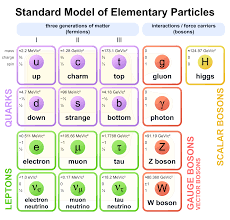
\includegraphics[width=0.7\textwidth]{figures/sm_blocks.png}
	\caption{The fundamental particles in the standard model of particle physics~\cite{StandardModel}.}
	\label{fig:sm}
\end{figure}



Fundamental particles are particles with no substructure. They are point particles with properties such as mass and spin. In the standard model, there are 17 fundamental particles. Of these, 12 are fermions - spin-1/2 particles - and 5 are bosons - integer-spin particles. 

The fermions are further classified into "quarks" and "leptons". Quarks have electromagnetic charge and color charge. Leptons have electroweak charge only. The properties of the leptons are described in Table~\ref{tab:leptons}, and the properties of the quarks are described in Table~\ref{tab:quarks}. 





Particles interact by exchanging force particles, all of which are spin-1 bosons in the Standard Model~\cite{martin}.


\begin{table}
\begin{center}
\begin{tabular}{||c c r c||} 
 \hline
 Particle & Mass [MeV] & Charge & Lifetime \\ [0.5ex] 
 \hline\hline
 $e^{-}$ & $0.511$ & $-1$ & Stable \\ 
 \hline
 $\nu_e$ & $<2$ & $0$ & Stable \\
 \hline
 $\mu^{-}$ & $105.7$ & $-1$ & $2.197 \times 10^{-6}$ \\
 \hline
 $\nu_\mu$ & $<0.19$ & $0$ & Stable \\
 \hline
 $\tau^{-}$ & $1777$ & $-1$ & $2.906 \times 10^{-13}$  \\
 \hline
 $\nu_\tau$ & $<18.2$ & $0$ & Stable \\ [1ex] 
 \hline
\end{tabular}
\end{center}
\caption{Mass, charge and lifetime of the leptons and lepton neutrinos~\cite{martin}.}
\label{tab:leptons}
\end{table}

\begin{table}
\begin{center}
\begin{tabular}{||c c r c||} 
 \hline
 Particle & Mass [GeV] & Charge & Lifetime \\ [0.5ex] 
 \hline\hline
 $u$ & $0.3$ & $2/3$ & Stable \\ 
 \hline
 $d$ & $0.3$ & $-1/3$ & Stable \\
 \hline
 $c$ & $1.5$ & $2/3$ & $10^{-12}$ \\
 \hline
 $s$ & $0.5$ & $-1/3$ & $10^{-8}$ \\
 \hline
 $t$ & $173$ & $2/3$ & $10^{-25}$  \\
 \hline
 $b$ & $4.5$ & $-1/3$ & $10^{-12}$ \\ [1ex] 
 \hline
\end{tabular}
\end{center}
\caption{Mass, charge and lifetime of the quarks~\cite{martin}.}
\label{tab:quarks}
\end{table}


The fermions are categorized into three generations; the first generation is represented by the first column in Figure~\ref{fig:sm}, the second generation is represented by the second row, and the third generation is represented by the third row. The generations are ordered by the masses of the quarks and leptons, and so the heavier generations can decay to the lighter generations, for example a muon can decay to an electron:

\begin{equation}
	\mu^{-} \rightarrow e^{-} + \bar{\nu}_e + \nu_\mu
\end{equation}

 The first generation particles do not have any known decays.


\subsection{Standard Model Forces}

The fermions interact with one another by exchanging spin-1 gauge bosons - the force carrying particles. The strong force is mediated by the gluon, the electromagnetic force is mediated by the photon, and the weak force is mediated by the $Z^0$ and $W^{\pm}$ bosons. 

\subsection*{Strong Force}

The strong force is described by Quantum Chromodynamics (QCD). QCD is a form of QFT with symmetry group SU(3). The force carriers, the gluons, are neutral particles that carry the color charge. There are three possible color charges: red, green, and blue. QCD obeys "color confinement", in which only color-neutral particles can exist. Color neutrality can be achieved by combing a red, green, and blue quark, or by combining a quark and anti quark of the same color (e.g. red and anti-red).

The particles in QCD also obey "asymptotic freedom", the property in which the strength of the strong force increases as distance increases. As the distance between the quarks in a $q\bar{q}$ increases, instead of the particles becoming isolated, a new $q\bar{q}$ pair is produced.

A QCD scattering interaction is shown in Figure~\ref{fig:feynman_qq}.

\begin{figure}[h!]
	\centering
	\feynmandiagram [vertical=a to b] {
	  i1 [particle=\(\color{red}{u}\)] -- [fermion] a -- [fermion] i2 [particle=\(\color{blue}{u}\)],
	  a -- [gluon, edge label'=\(g\)] b,
 	 f1 [particle=\(\color{red}{s}\)] -- [anti fermion] b -- [anti fermion] f2 [particle=\(\color{blue}{s}\)],
	};
	\caption{$qq$ scattering with an up quark with red color charge and a strange quark with blue color charge.}
	\label{fig:feynman_qq}
\end{figure} 



\subsection*{Electromagnetic Force}

The electromagnetic force is mediated by the photon, which carries the electric charge ($\pm 1$) and only acts on charged particles. The electromagnetic force is described by Quantum Electrodynamics (QED), which has a coupling strength $\alpha \approx 1/137$. In QED, particles obey the "Pauli Exclusion Principle": no two fermions can inhabit the same quantum state. An electromagnetic scattering interaction is shown in Figure~\ref{fig:feynman_ee}.

\begin{figure}[h]
	\centering
	\feynmandiagram [vertical=a to b] {
	  i1 [particle=\(e^{-}\)] -- [fermion] a -- [fermion] i2 [particle=\(e^{-}\)],
	  a -- [photon, edge label'=\(\gamma\)] b,
 	 f1 [particle=\(\mu^{-}\)] -- [anti fermion] b -- [anti fermion] f2 [particle=\(\mu^{-}\)],
	};
	\caption{An electron muon scattering interaction with scattering amplitude $e^2/q^2$ for a 1 photon exchange interaction.}
	\label{fig:feynman_ee}
\end{figure}



\subsection*{Weak Force}

All fermions can interact through the weak force. The weak force is so named because it is the weakest of the three standard model forces with a coupling strength $a_W \approx 10^{-6}$ (gravity, which is not in the standard model, is weaker than the weak force). Lepton neutrinos interact through the weak force only.




\section{Electroweak Symmetry Breaking}

The electroweak interaction is a unified description of the electromagnetic and weak forces. It is based on the symmetry groups $SU(2)_L \times U(1)_Y$. At high temperatures corresponding to an energy of 246 GeV, the electromagnetic and weak forces can be described by one force. Experiments finding the W and Z bosons confirmed some of the predictions of the theory. The electroweak force has four bosons before symmetry breaking occurs ($W_1$, $W_2$, $W_3$ and $B$). After electroweak symmetry breaking, the $W$ boson is a combination of the first 2 electroweak bosons (Equation~\ref{eq:w}) and the photon and $W$ and $Z$ bosons are a combination of the latter 2 (Equation~\ref{eq:zgamma}

\begin{equation}
	W^{\pm} = \frac{1}{\sqrt{2}}
	\begin{pmatrix}
		W_1 \mp iW_2
	\end{pmatrix}
	\label{eq:w}
\end{equation}


\begin{equation}
	\begin{pmatrix}
		\gamma \\
		Z 
	\end{pmatrix} = \begin{pmatrix}
		\cos{\theta_W} & \sin{\theta_W} \\
		-\sin{\theta_W} & \cos{\theta_W}
	\end{pmatrix}
	\begin{pmatrix}
		B \\
		W_3 
	\end{pmatrix}
	\label{eq:zgamma}
\end{equation}

where $\theta_W$ is the weak mixing angle, or "Weinberg angle", which is the angle relating $g'$ to $g$, the hypercharge and isospin, respectively, of the weak interaction (see Figure~\ref{fig:weinberg}).

\begin{figure}[htbp!]
	\centering
	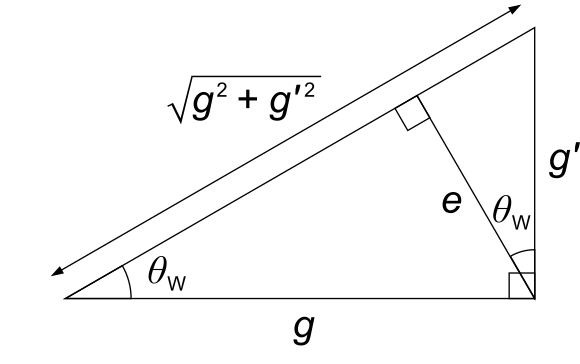
\includegraphics[width=0.4\textwidth]{figures/Weinberg_angle.png}
	\caption{The weak mixing angle $\theta_W$ is the angle relating $g'$ to $g$.}
	\label{fig:weinberg}
\end{figure}


\subsection*{Higgs Mechanism}

The Higgs boson, the spin-0 scalar boson of the standard model, is responsible for electroweak symmetry breaking through the "Higgs Mechanism". The Higgs Mechanism is the term for the $SU(2)_L \times U(1)_Y$ symmetry of the electroweak force breaking into the the $U(1)$ of the electromagnetic force.


The Higgs Mechanism was proposed in 1964~\cite{higgs}. Collider experiments since searched for the Higgs particle, whose mass was not known from theoretical predictions. The Higgs boson was not detected until 2012, when the CMS and ATLAS experiments at the LHC published separate 


\section{Beyond the Standard Model}


The Standard Model is incomplete. It does not contain gravity, which is much weaker than the weak force. The matter described by the standard model makes up only 5\% of the known matter in the universe, the rest is Dark Matter (matter that does not interact with Standard Model particles but does interact gravitationally) and Dark Energy, which is responsible for the acceleration of the expansion of the universe. Theoretical models attempt to solve these problems. 


\subsection*{Extra Dimensions}


\begin{figure}[h!]
	\centering
	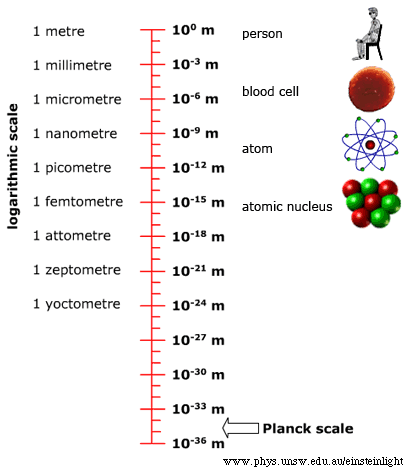
\includegraphics[width=0.5\textwidth]{figures/Planck_scale.png}
	\caption{Logarithmic scale of standard model forces and Planck scale~\cite{Planck_scale}.}
	\label{fig:planck}
\end{figure}


The orders of magnitude difference between the Planck scale and the electroweak scale is called the "Hierarchy Problem". Theoretical predictions suggest that the mass of the Higgs boson should be much larger than its $m_H \approx 125$ GeV. The heaviest fundamental particle is the top quark, at $m_t \approx 173$ GeV, which is on the order of the electroweak scale ($\approx 100$ GeV). A possible answer to this discrepancy is to search for new, heavier particles at the highest energy scales possible at the LHC that decay to $t\bar{t}$ pairs. 

The Randall Sundrum (RS1) model is a theoretical framework with a fourth spatial dimension, with a 3 dimensional brane on the electroweak scale and a 1 dimensional brane on the Planck scale~\cite{rs1}. Figure~\ref{fig:rsbrane} shows a diagram of this RS1 model, where the scale of gravity decreases when moving from the UV brane to the IR brane. The model proposes a graviton that is on the TeV scale, and decays to $t\bar{t}$. A second Randall-Sundrum model (RS2) proposes a fourth spatial dimension but only one TeV-scale brane~\cite{rs2}.

\begin{figure}[h]
	\centering
	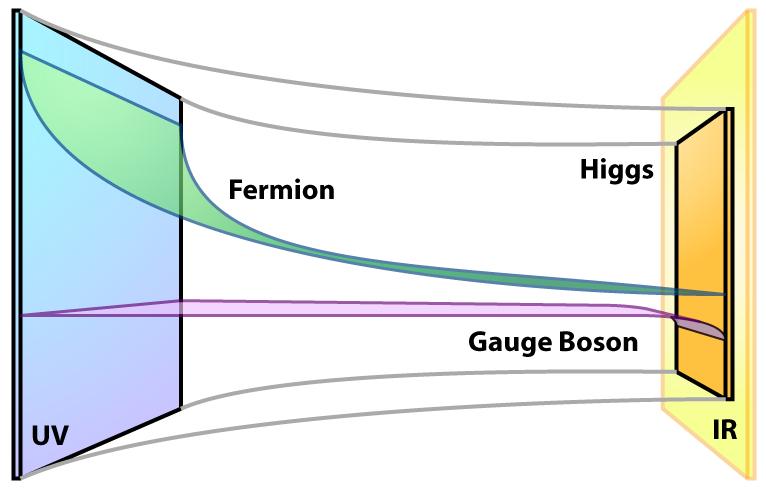
\includegraphics[width=0.75\textwidth]{figures/RSBrane.png}
	\caption{The extra spatial dimensions proposed in the Randall-Sundrum model~\cite{RSBrane}.}
	\label{fig:rsbrane}
\end{figure}



%
%\subsection*{Dark Matter}
%
%
%Simplified Dark Matter models propose a $Z'$ boson that decays to $t\bar{t}$~\cite{simplified_dm}.
%
%
%
%\subsection*{Leptophobic Topcolor Resonances}
%
%
%\section{Monte Carlo Simulation}
%
%
%For simulations of QCD in pp collisions on the energy scales of the LHC, several methods of calculation are combined. For the energy scale $\mu^2$ > 1 GeV, part
%
%\begin{figure}[h]
%	\centering
%	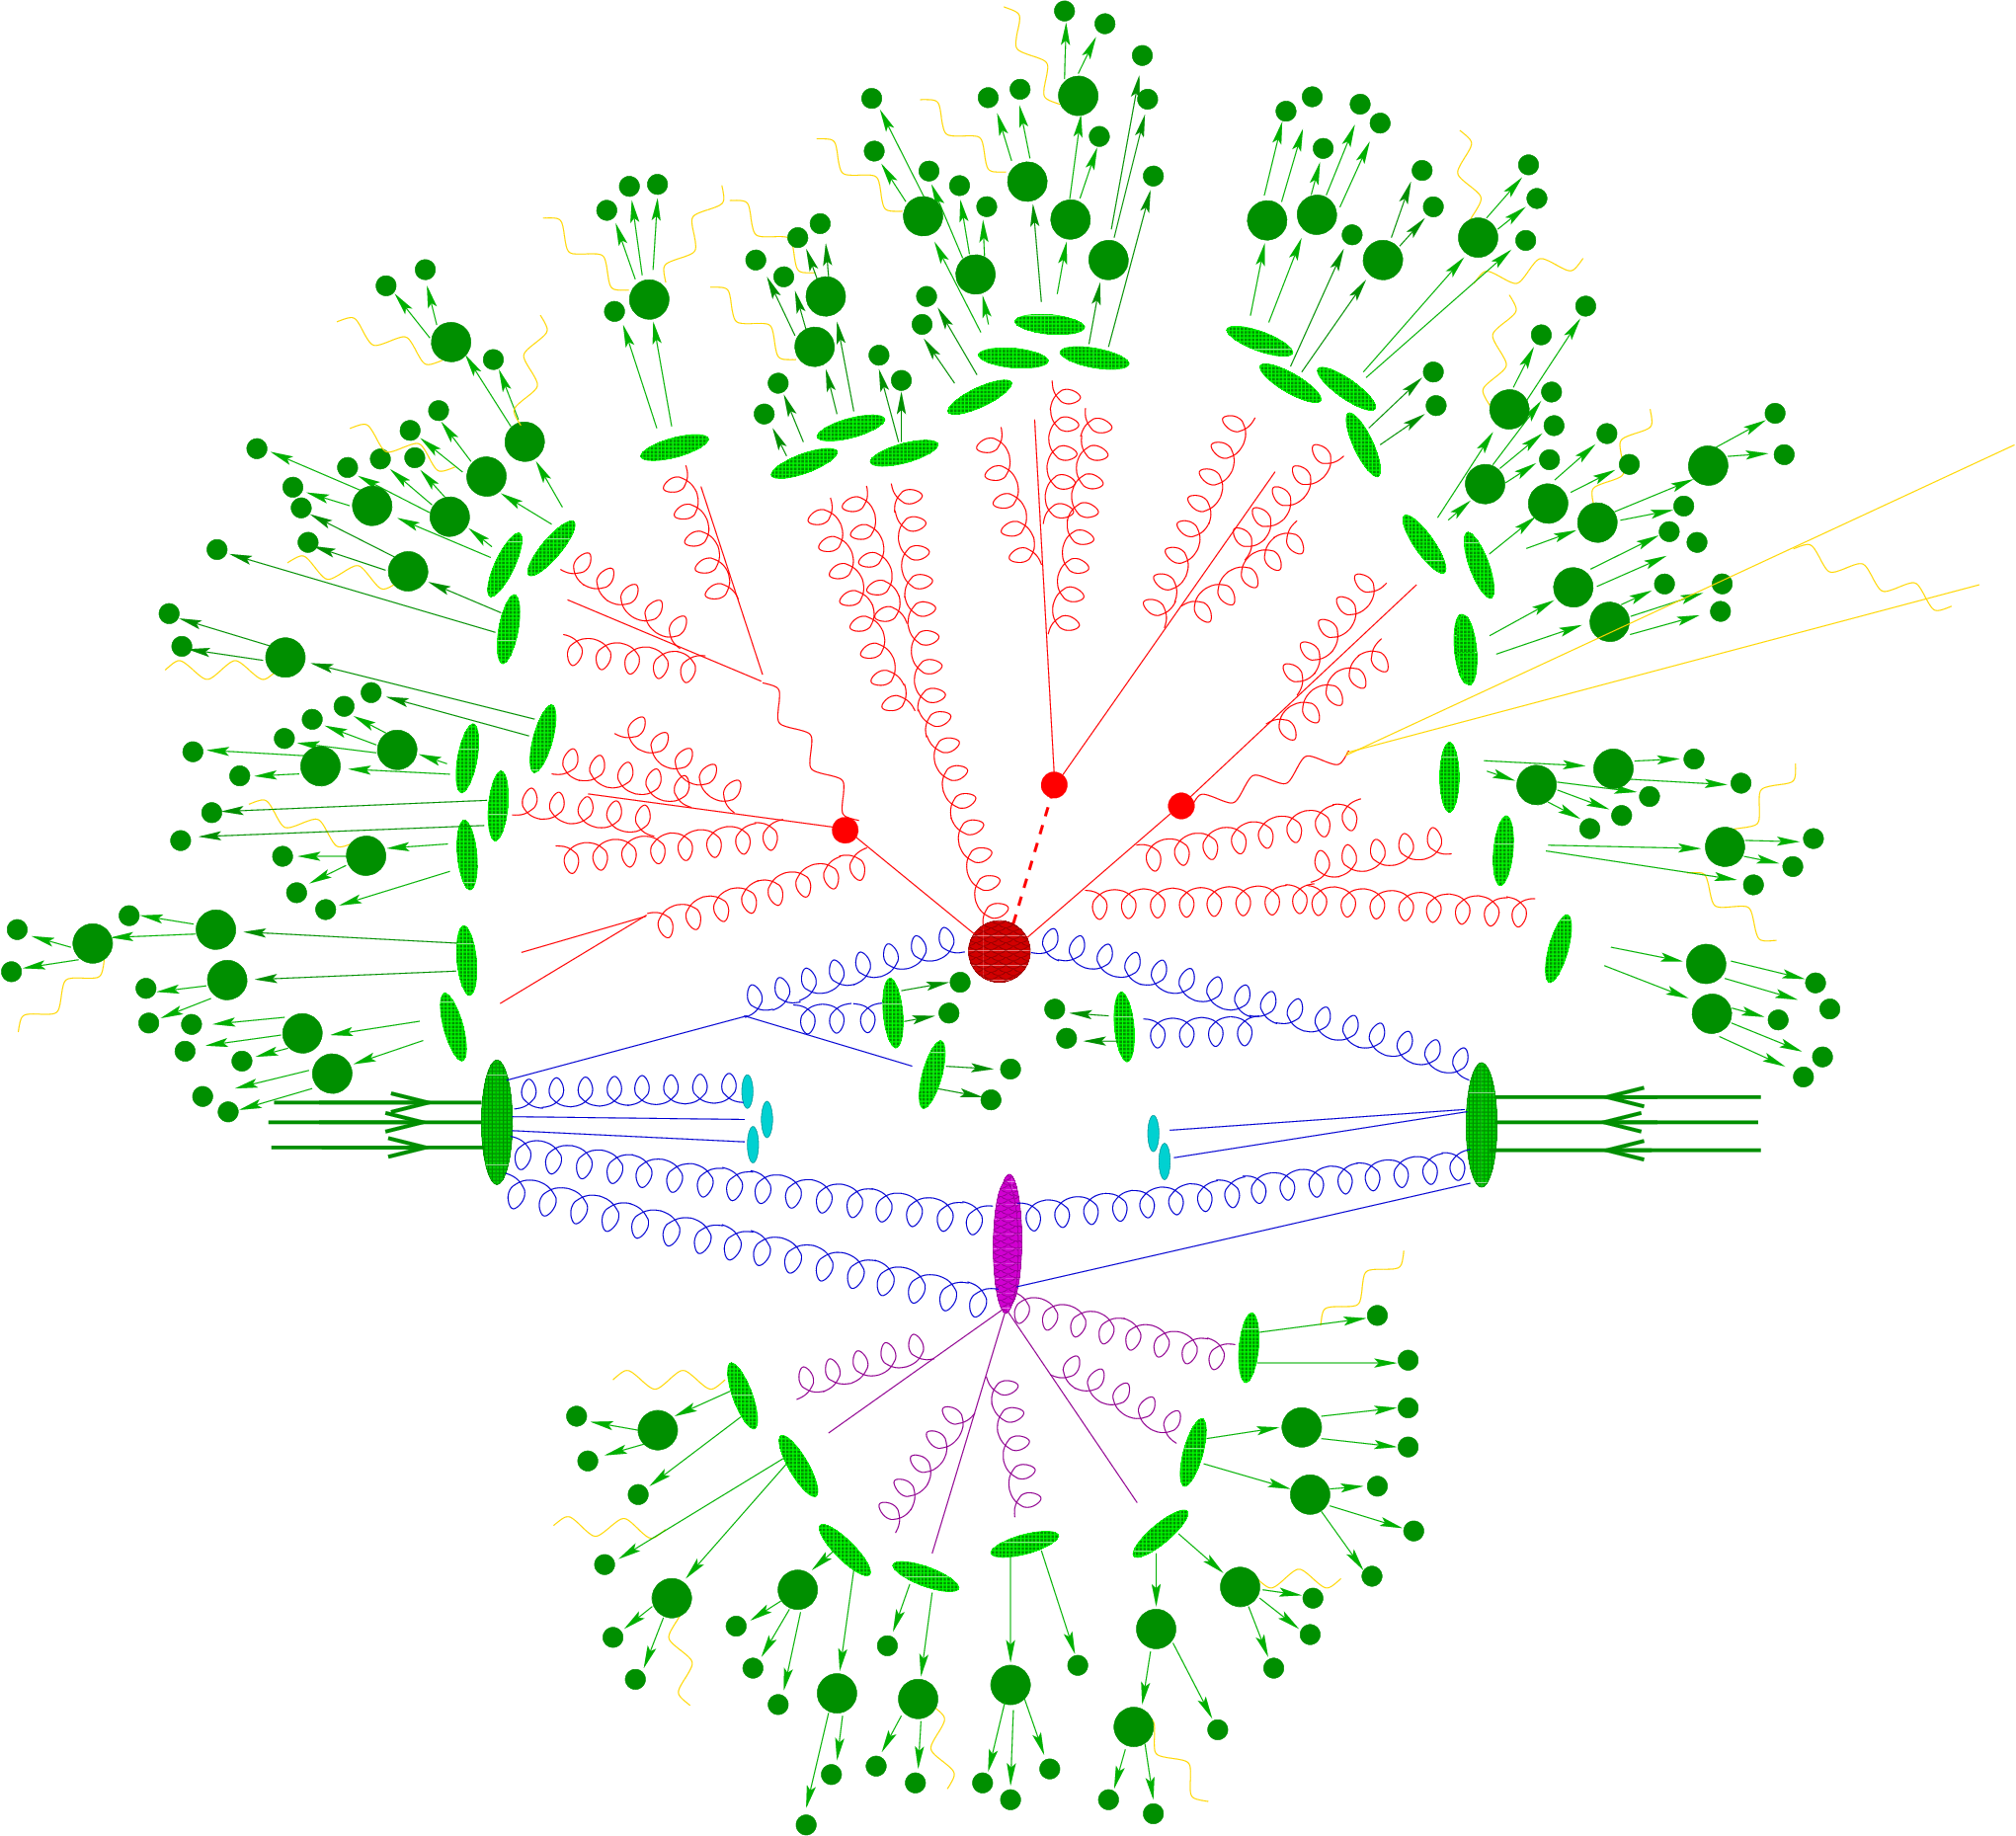
\includegraphics[width=0.65\textwidth]{figures/parton_shower.png}
%	\caption{Diagram of a parton shower from a pp collison~\cite{PartonShower}.}
%	\label{fig:ps}
%\end{figure}
%
%\begin{figure}[h]
%	\centering
%	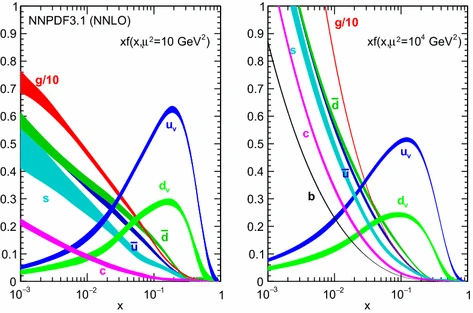
\includegraphics[width=0.65\textwidth]{figures/pdf_lhc.png}
%	\caption{Diagram of a parton shower from a pp collison~\cite{pdfs}.}
%	\label{fig:ps}
%\end{figure}
%


%\begin{itemize}
%	\item PDFs
%	\item ME + PS + hadronization
%\end{itemize}

\chapter{The CMS Detector}\label{chap:cms}


% \vspace{-5pt}
\section{Introduction}\label{sec:ch3:intro}

 \begin{figure}[h]
\centering
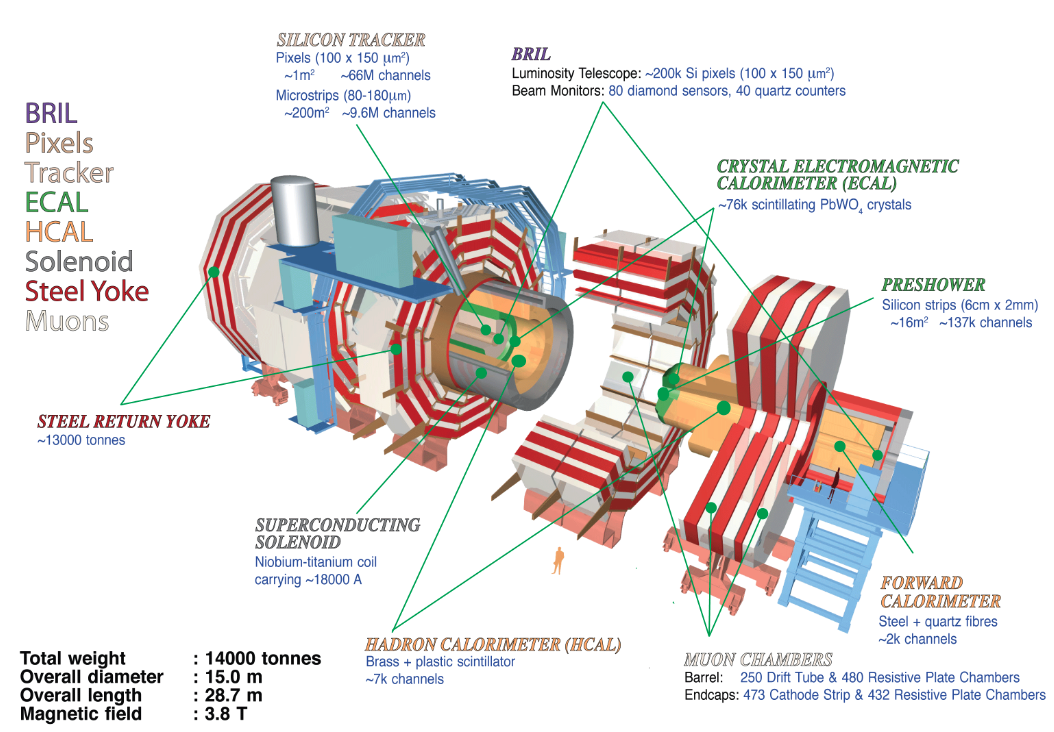
\includegraphics[width=0.8\textwidth]{figures/cms_schematic.png}
\caption{Schematic of the Compact Muon Solenoid (CMS) detector~\cite{cms_schematic}.}
\label{fig:cms}
\end{figure}

Figure \ref{fig:cms} shows the schematic of the Compact Muon Solenoid (CMS) detector. The detector is located in the Large Hadron Collider (LHC), which is depicted in the collider apparatus in Figure \ref{fig:cern}.

 \begin{figure}[h]
\centering
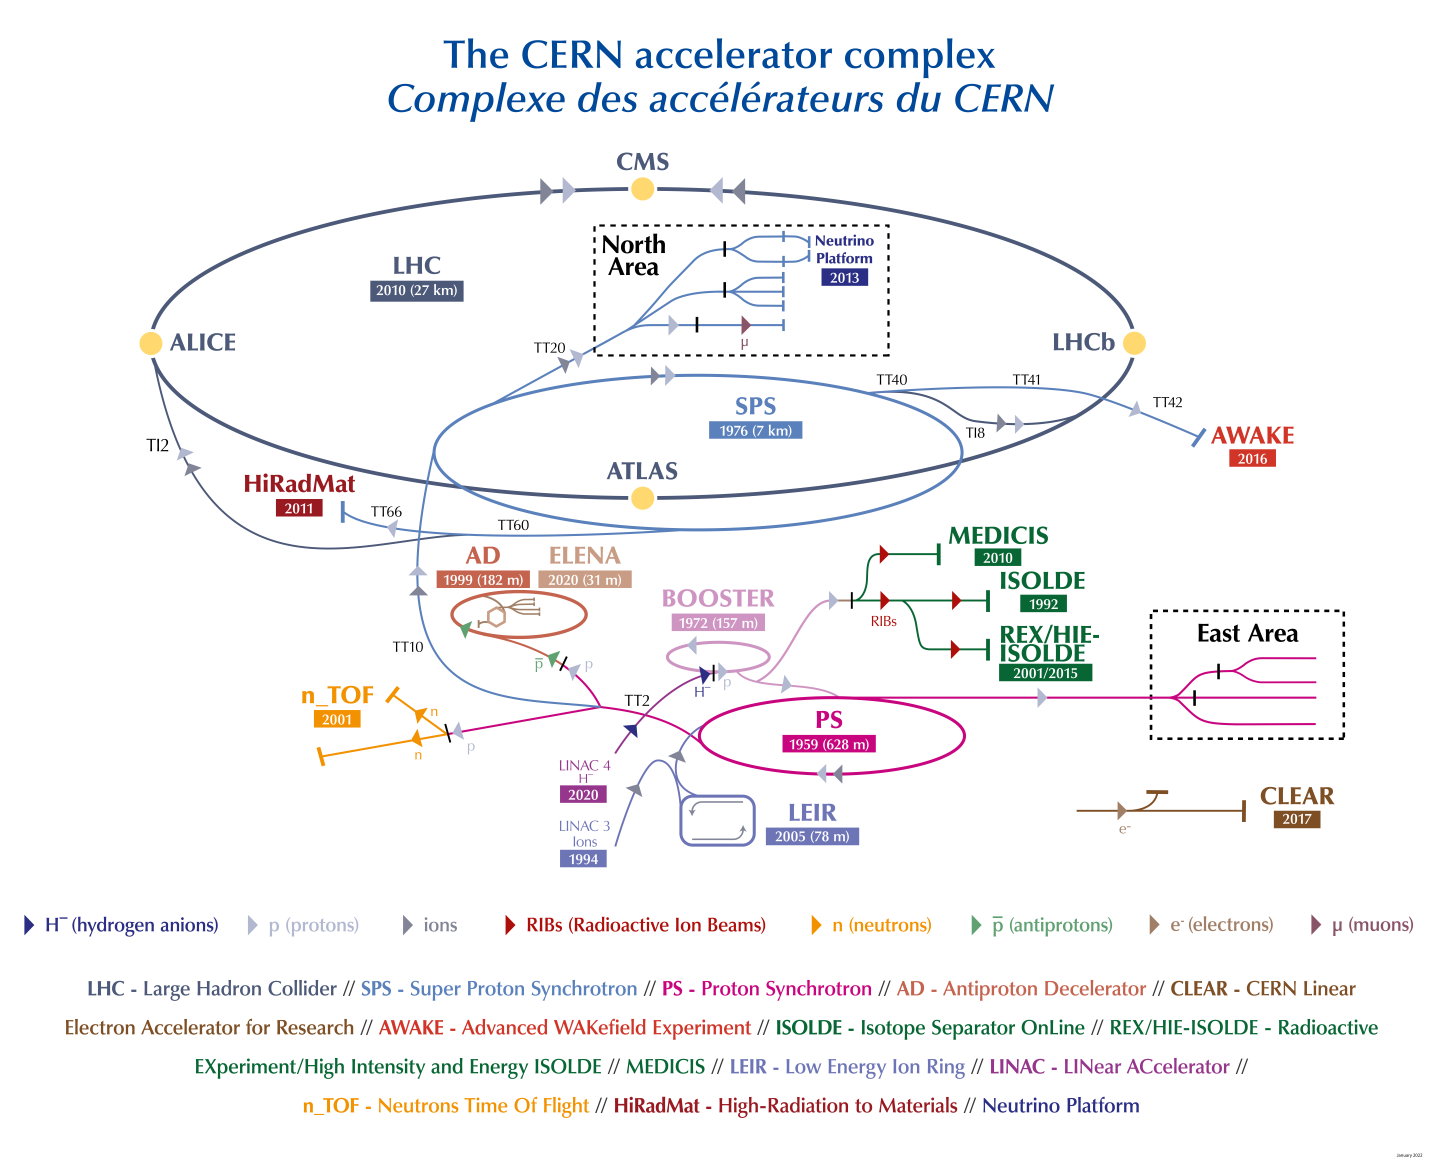
\includegraphics[width=1.0\textwidth]{figures/CCC-v2022.png}
\caption{Schematic of the collider apparatus at CERN~\cite{CERN_Accelerator_Complex}.}
\label{fig:cern}
\end{figure}


The Large Hadron Collider (LHC) beam energy, originally at 7 TeV, now for Run 3 at 13.6 TeV, allows us to study physics at the highest energy scale ever in a laboratory setting. The collaboration also performs studies of heavy ions at 30x the energy of previous heavy ion experiments. With a luminosity for pp collisions 100x greater than previous experiments, and pp cross section of about 100 mb, measurements can be done to greater precision than ever before, and searches can probe the highest ever possible masses at the TeV scale.

The LHC contains multiple experiments. At opposite points of the collider, 27 km apart, sit ATLAS (or the experiment formerly known as A ToroidaL ApparatuS) and the Compact Muon Solenoid (CMS) experiments. The experiments perform similar searches and measurements without sharing preliminary results. This mitigates biases from experimentalists during the analyses.

The CMS detector is located at Point 5 at the Large Hadron Collider~\cite{CMSExperiment}. It has several subsystems, including the tracker, the electromagnetic calorimeter, the hadronic calorimeter, the solenoid, and the muon chambers. The CMS detector is cylindrical and so each detector has a cylindrical "barrel" region and disk-shaped "endcap" region. The Endcap regions are necessary as nearly $1/3$ of all particles cross the $1.3 < |\eta| < 3$ region.

\vspace{-3pt}
\section{The Tracker}\label{sec:ch3:trk}


\begin{figure}[h]
\centering
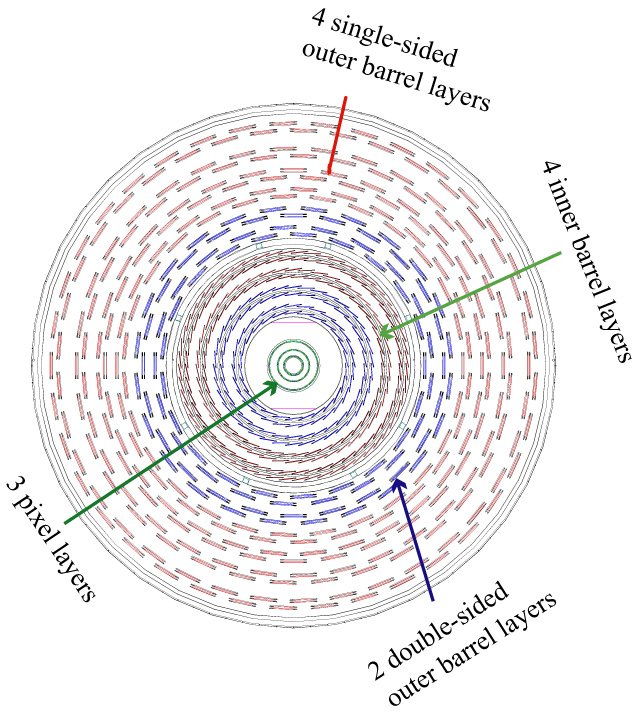
\includegraphics[width=0.5\textwidth]{figures/Barrel_0_tracker.png}
\caption{Schematic of the tracker.}
\label{fig:tracker_circular_schematic}
\end{figure}

 \begin{figure}[h]
\centering
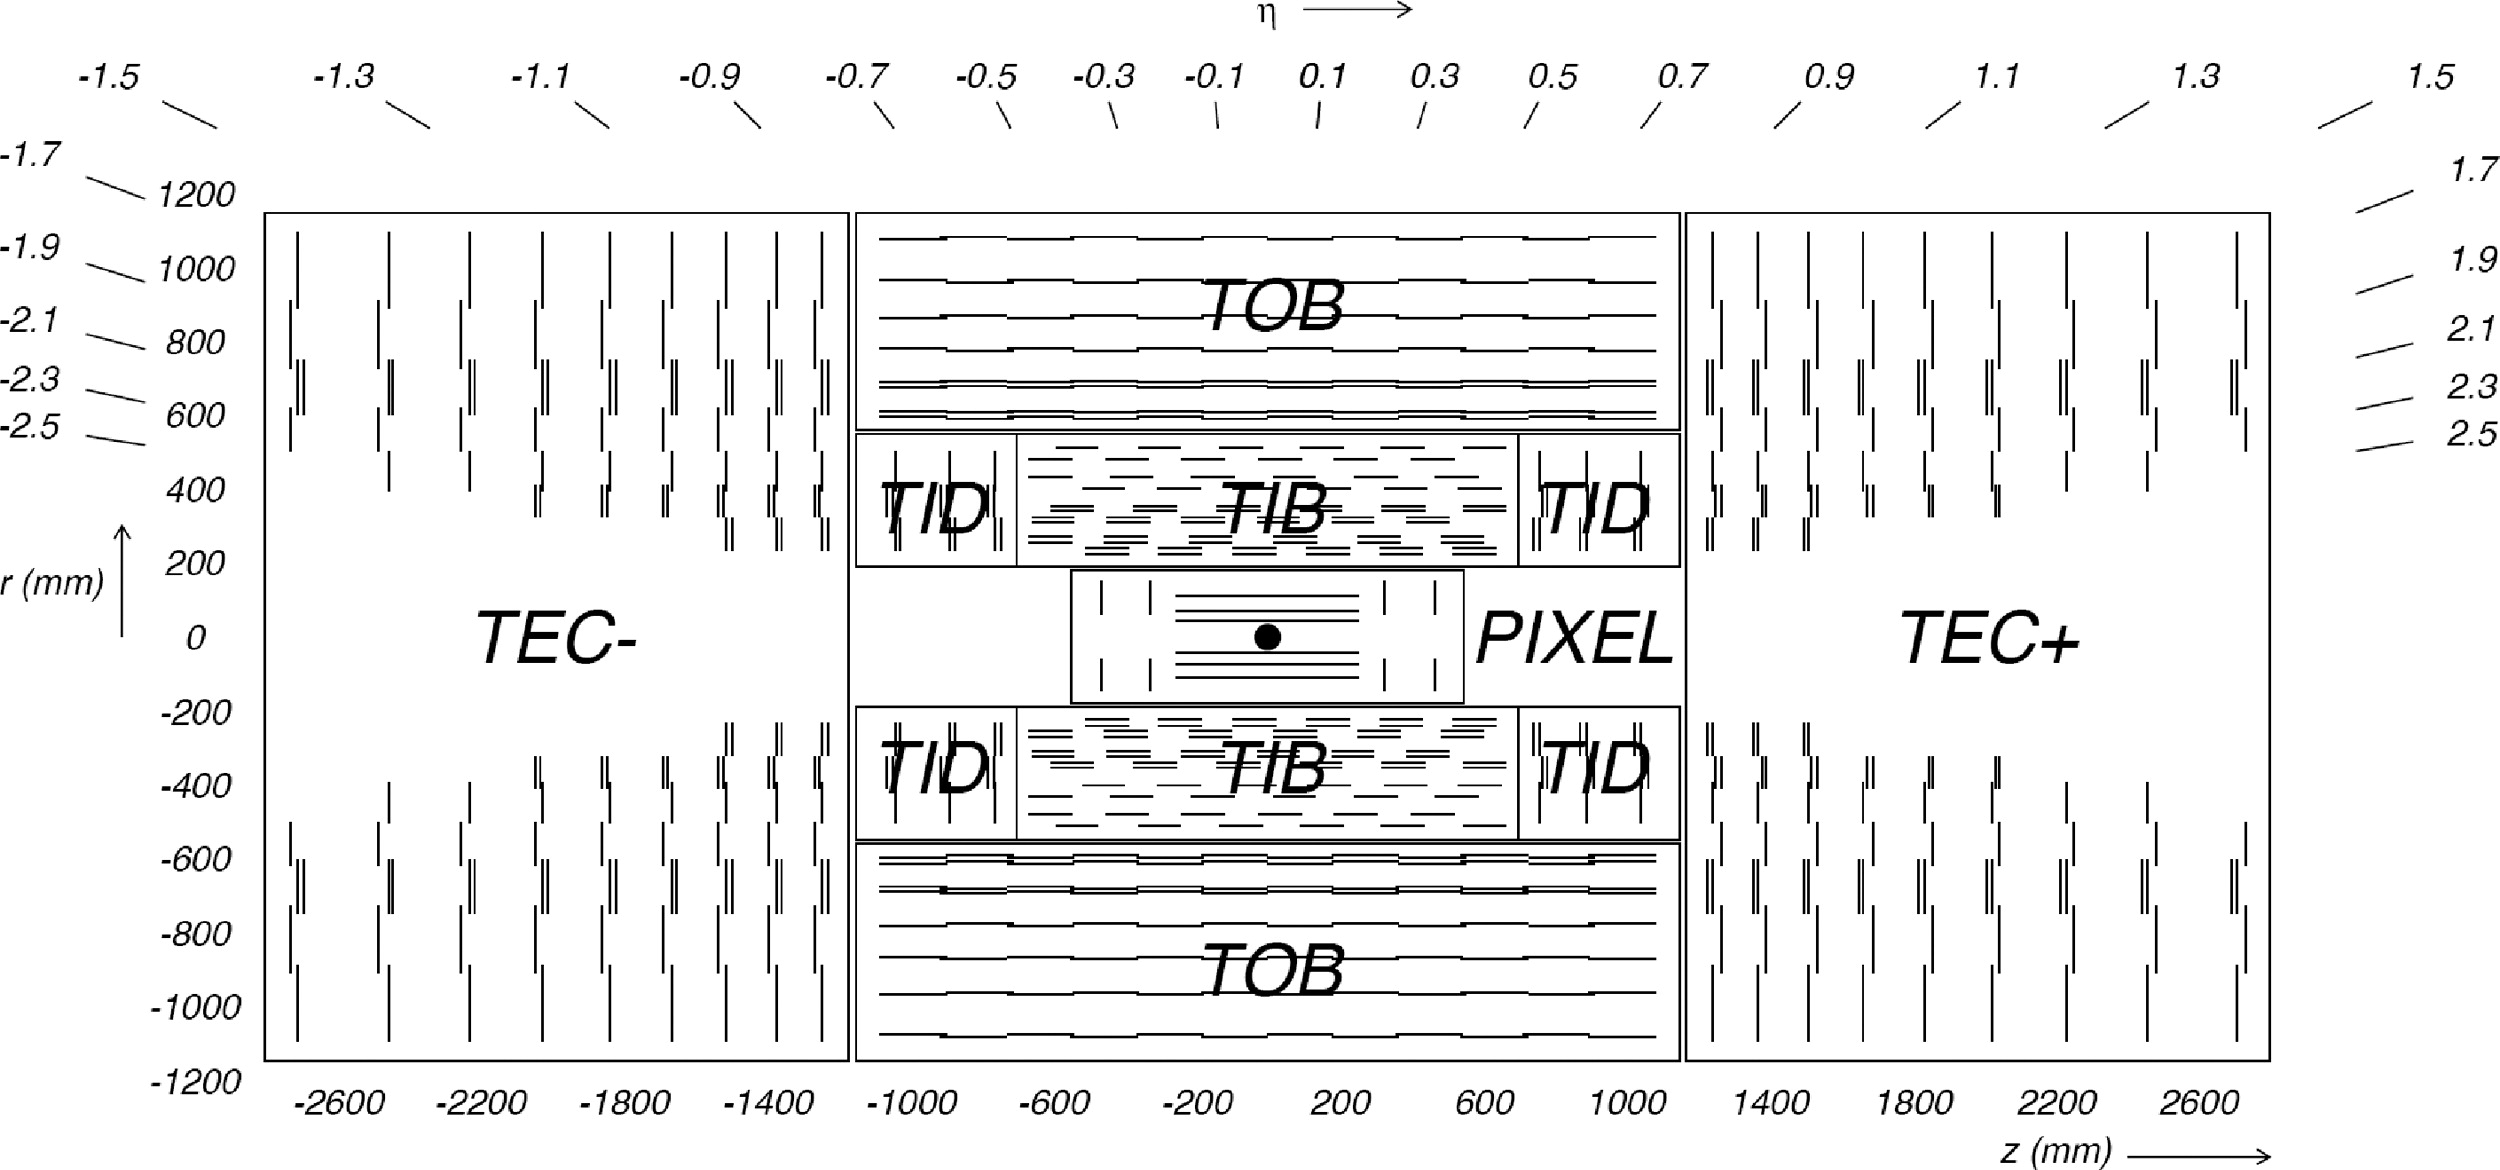
\includegraphics[width=1.0\textwidth]{figures/cms_tracker_cross_section_schematic.jpg}
\caption{Schematic of the tracker, projected onto an $z$-$r$ plane.}
\label{fig:cms_tracker_cross_section_schematic}
\end{figure}

At the innermost layer of the detector, held within the 6 meter bore of the solenoid, sits the silicon tracking system. With 1000 particles from 20 overlapping collisions bombarding the detector every 25 ns, the tracker needs a high power density system to accurately and precisely measure the tracks of individual charged particles. The high energy particles subject the electronics to high radiation levels. A radiation-hard material cooled to low temperatures is needed to withstand these high levels. For this, silicon was used, and has tracker has been operating for over a decade, longer than the planned lifetime of the detector. The tracker was built over the course of over a decade, with the input of hundreds of particle physicists from 51 institutes, including the University at Buffalo.


The tracker is composed of two subdetectors: an inner 3-layer pixel detector pixel detector and an outer 10-layer strips detector. inner , with 10 barrel layers of silicon strip tracking. In Figure~\ref{fig:tracker_circular_schematic}, the positions of these layers are shown on a circular cross-section of the cylindrical Tracker. Inside the innermost circle is the beam line where the interaction point for the detector sits. This interaction point is depicted as a black dot in Figure~\ref{fig:cms_tracker_cross_section_schematic}, which shows the detector projected onto an $r$, $z$ plane.  The 3 barrel layers of the pixel detector are the 3 lines above and below the interaction point. The pixel barrel (BPix) is 53 cm long with the largest radius at 10.2 cm, which allows coverage of $|\eta| > 2.5$. The pixel front endcaps (FPix) are position in 2 layers at $|z| = 34.5$ cm and $|z| = 46.5$ cm. The pixel layers have high granularity to allow for precise measurement of the position of the detected particles. Each pixel has an area of $100x150$ \textmu m, with 48 million pixels in BPix and 18 million in FPix~\cite{CMSExperiment}.

The strip tracker surrounds the pixel subdetector. In Figure~\ref{fig:cms_tracker_cross_section_schematic}, the subdetectors for the strips tracker are shown. The tracker inner barrel (TIB) has 4 layers with 320 \textmu m thick silicon strip sensors. The tracker outer barrel (TOB) has 6 layers with 500 \textmu m thick silicon strip sensors. The tracker has disk layers covering the high $|\eta|$ region. The tracker inner disks (TID) have 3 layers, and the tracker endcaps (TEC) have 8 layers. The TEC, TID, and FPix disk layers and the TOB, TIB, and Bpix barrel layers supply a total of 22 measurements with resolutions ranging from 23 \textmu m to 53 \textmu m, further described in Table~\ref{tab:rphi_mmts}.

\begin{figure}[h]
\centering
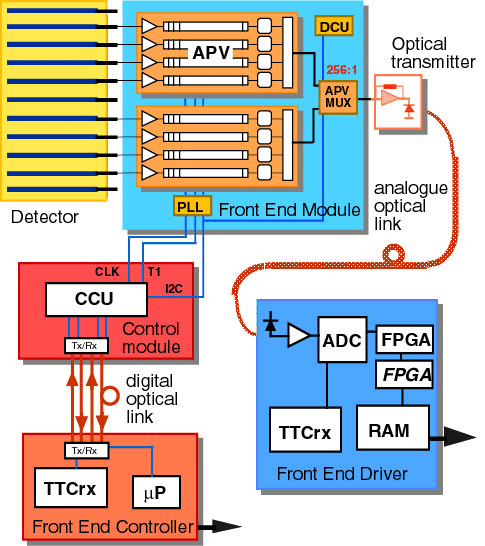
\includegraphics[width=0.5\textwidth]{figures/Read-out-scheme-of-the-CMS-Tracker.png}
\caption{Schematic of the tracker readout system~\cite{CMSExperiment}.} \label{fig:tracker_readout}
\end{figure}

\begin{table}
\begin{center}
\begin{tabular}{||c c c||} 
 \hline
 Subdetector & Resolution & $r-\phi$ Measurments \\ [0.5ex] 
 \hline\hline
 BPix/FPix &  & 3 \\ 
 \hline
 TIB/TID & 23-25 \textmu m & 4 \\
 \hline
 TOB & 35-53 \textmu m  & 6 \\
 \hline
 TEC &  & 9 \\ [1ex] 
 \hline
\end{tabular}
\caption{Resolution of the pixel and strips subdetectors with the number of measurements in $r-\phi$ each supplies~\cite{CMSExperiment}.}
\label{tab:rphi_mmts}
\end{center}
\end{table}
%
%\begin{todolist}
%	\item describe silicon strip sensors
%\end{todolist}


The tracker materials must be kept to low temperatures to mitigate the damage caused by the radiation from the beam collisions. Cooling liquid is transported to the silicon sensors by aluminum pipes, which are formed into cooling loops and attached to the sensors with aluminum ledges.

The information from the silicon sensor is sent through a readout system, shown in Figure~\ref{fig:tracker_readout}. Fiber optic cables carry analog signals from the sensors in the tracker to Front End Drivers (FEDs). The FEDs convert the analog signals to digital. Front End Controllers (FECs) transmit signals from the clock, control systems, and trigger. The information from the tracker is vital to the high level trigger (HLT) decisions, which reduce the rate of incoming collisions data by a factor of 400. Silicon modules contain either one of the 320 \textmu m or 2 of the 500 \textmu m thick silicon sensors. The modules are grouped into power groups that are each powered by one power supply, which supplies 2 low voltage lines at 1.25 V and 2.5 V, and 2 high voltage lines. The silicon sensors are made of p-on-n type material. On the back, n type aluminum is used to connect to a positive voltage. On the other side are the p+ type silicon strip diodes. 

The Detector Control Systems (DCS) are designed using a Supervising Control and Data Acquisition (SCADA) program developed with WinCCOA. The DCS is a Final State Machine tree that controls all of the power supplies. A Detector Control Unit monitors the low voltage, leakage current, and temperature of the silicon sensors.

The radiation length of materials used in the tracker shown in Figure~\ref{fig:tracker_radiation_length.}.

\begin{figure}[h]
\centering
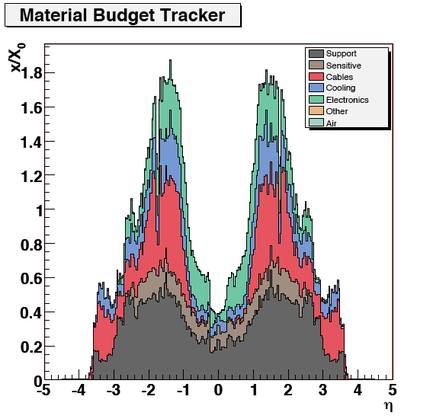
\includegraphics[width=0.5\textwidth]{figures/tracker_radiation_length_XoverX0.png}
\caption{Radiation length of materials used in the tracker~\cite{CMSExperiment}.}
\label{fig:tracker_radiation_length.}
\end{figure}



\vspace{-3pt}
\section{The Electromagnetic Calorimeter}\label{sec:ch3:ecal}

The Electromagnetic Calorimeter (ECAL) surrounds the tracker. Its purpose is to absorb the energy from electrons and photons, and was built with the motivation of detecting the decay of two photons for Higgs boson searches. The ECAL is composed of thousands of lead tungstate (PbWO$_4$) crystals, which are mounted on a barrel layer and two endcaps. Before the endcaps, a preshower made of two planes of lead reduces false signals.

Lead tungstate crystals are useful in a compact detector because they are radiation-hard and have a small radiation length and small Moliere radius. Additionally, the scintillation decay time of lead tungstate is approximately 25ns, which is the same as the bunch crossing separation in the LHC. The barrel receives the particle data through avalanche photodiodes, which apply a reverse bias voltage to get a current gain effect of about 50. The endcaps use vacuum phototriodes, which are photomultipliers with a single gain state. The vacuum phototriodes usee in the ECAL were developed specifically for CMS, and are useful in the endcaps because they are more radiation resistant than diodes.

The barrel of the ECAL covers $|\eta| < 1.479$, and the endcaps cover $1.479 < |\eta| < 3.0 $. Water cools the submodules containing the crystals at a temperature of 18$^{\circ}$C.


The energy resolution in the ECAL is described by Equation \ref{eq:ecal1}.

\begin{equation}
\left( \frac{\sigma}{E} \right)^2 = \left( \frac{S}{\sqrt{E}} + \left( \frac{N}{E} \right)^2\right)^2 + C^2
\label{eq:ecal1}
\end{equation}

$S$ is the stochastic term, and is comprised of photostatistics (about 2.1\%), fluctuations in energy deposited in the preshower (about 5\%/$\sqrt{E}$), and fluctuations in the lateral shower containment (about 1.5\%). $N$ is the noise term, and is comprised of electronics, digitization, and pileup noise. $C$ is the constant term, and is made up of leakage from the back of the crystals, intercalibration errors, and non-uniformity in light collection, the last being less than a 0.3\% contribution.

\vspace{-3pt}
\section{The Hadron Calorimeter}\label{sec:ch3:hcal}

\begin{figure}[h]
\centering
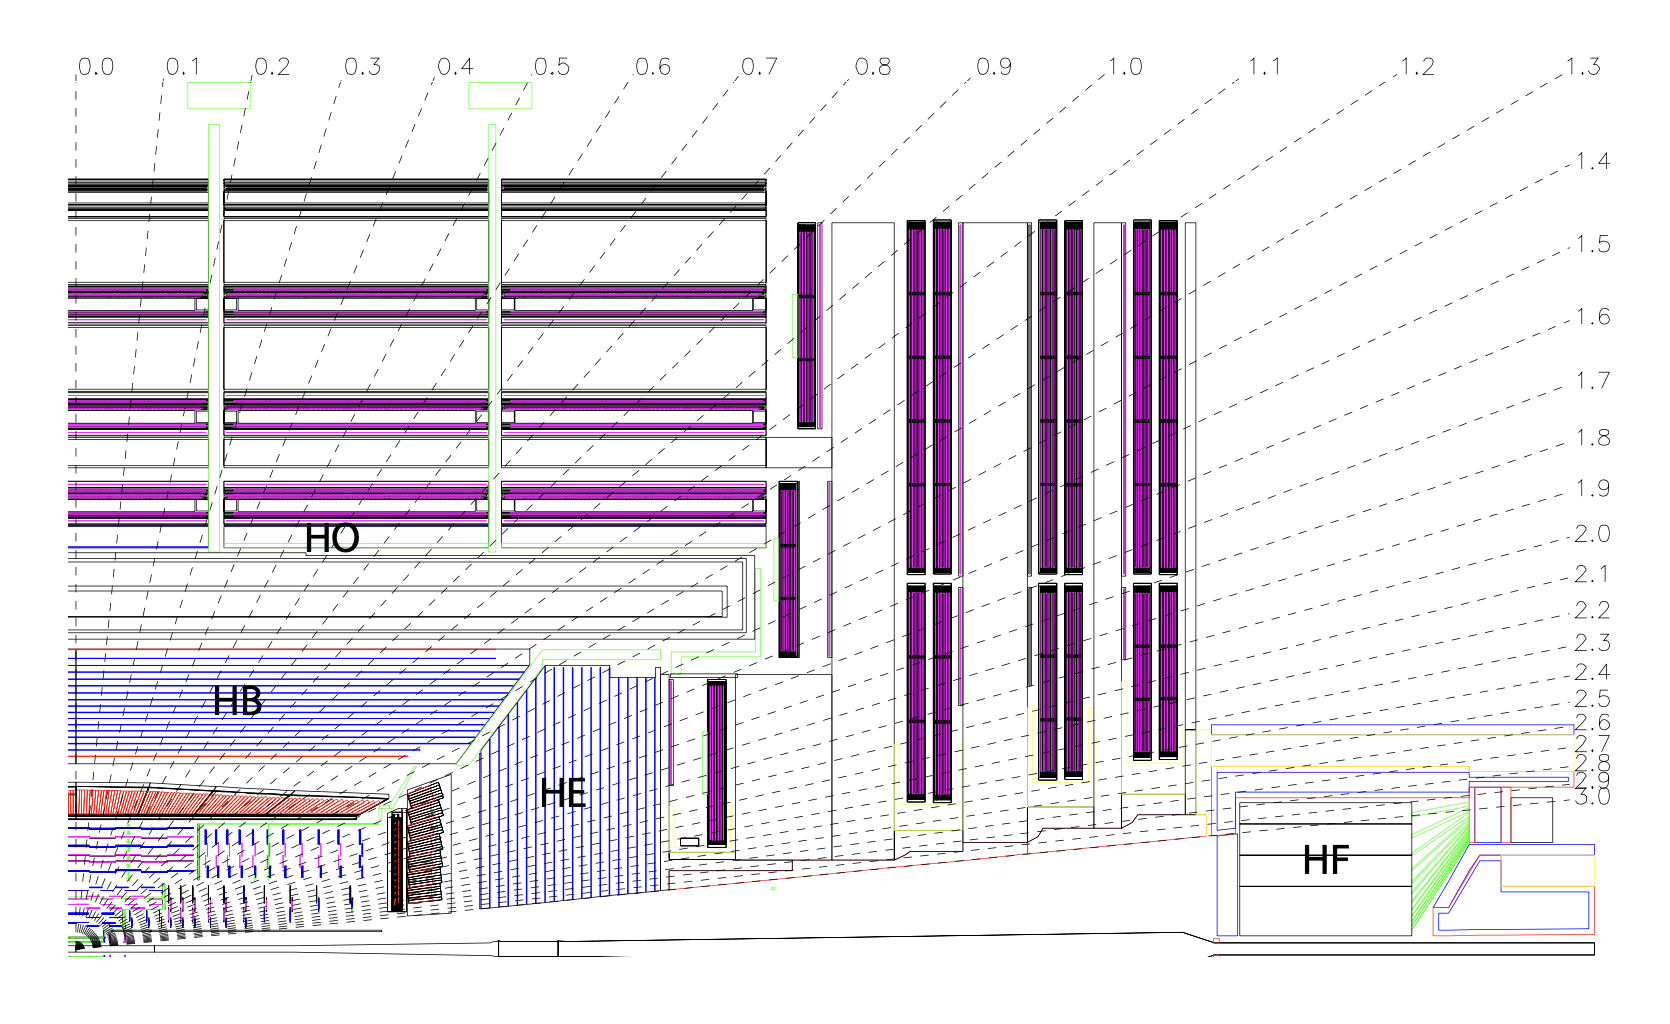
\includegraphics[width=1.0\textwidth]{figures/HCAL.png}
\caption{Schematic of the Hadron Calorimeter.}
\label{fig:HCAL}
\end{figure}


\begin{figure}[h]
\centering
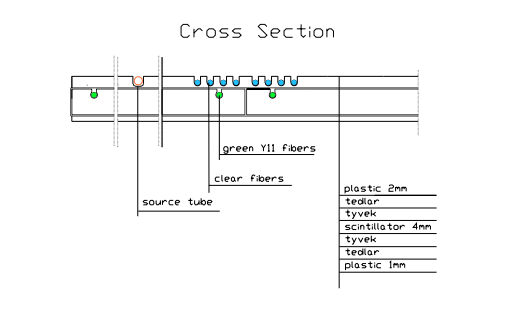
\includegraphics[width=1.0\textwidth]{figures/hcal_scintillator_replace.png}
\caption{Schematic of the plastic scintillator in the HCAL.}
\label{fig:HCAL_scint}
\end{figure}

The Hadron Calorimeter (HCAL) is designed to absorb the energy from the hadronic particles. It is split in four sections: the barrel (HB), the endcap (HE), the outer calorimeter (HO), and the forward calorimeter (HF), shown in Figure~\ref{fig:HCAL}. The barrel (HB), covers $|\eta| < 1.3$, and the endcaps (HE), cover $1.3 < |\eta| < 3.0$. The HB is a sampling calorimeter of absorber (bronze) and scintillator (plastic). The brass absorber is divided into 36 wedges in $\phi$. The plastic scintillator is divided into 16 sectors in $\eta$. The brass absorber is used for it's cost, radiation hardness, and non-magnetic properties.

The HCAL has a limited distance between the ECAL and the solenoid to absorb the hadronic particles. For particles that are unable to be stopped in that distance, an outer calorimeter is placed outside the solenoid in the central eta region



Hadrons penetrate more material than electrons and photons. Some hadrons still are not completely absorbed by the HCAL subdetectors between the ECAL and solenoid. Therefore the HO is set outside of the solenoid at R = 4.07 to catch any hadrons that are not stopped by the HB or HE. The HB is a sampling calorimeter with alternating layers of brass absorber and plastic scintillator. The brass absorber plates in the HB are positioned parallel to the beam line in a staggered formation. The first and last layer of the HB is a steel to serve as both an absorber layer and to provide structural strength. The HB has a total absorber length of 5.82 $\lambda_I$, where $\lambda_I$ is the interaction length of hadronic particles. The interaction length increases with $\theta$ as $1/\sin{\theta}$, for an thickness of 5.82 $\lambda_I$ at the edge of the HB at $|\eta| = 1.3$.

The scintillators are made of the material Kuraray SCSN81, which is a stable and radiation hard plastic. The plastic is formed into 70,000 tiles which are layered in trays between the brass absorber plates. One layer plastic scintillator sits in front of the steel absorber and one behind to catch any showers that start before the HCAL or that leak out the start of the HCAL. Tubes carry radioactive material through the plastic scintillator tiles for Cs$^{137}$ for calibration. A schematic of the plastic scintillator is shown in Figure~\ref{fig:HCAL_scint}.

The plastic scintillators detect the hadrons which are stopped by the brass absorbers. When a hadronic particle enters the plastic scintillator, the photoelectrons ionize and experience a gain of 2000 in the diode. Fiber optic cables in the scintillator carry the light to clear fiber. optic cables which carry the light to the photodiode. A diagram of a generic scintillator is shown in Figure~\ref{fig:scintillator}.

\begin{figure}[h]
\centering
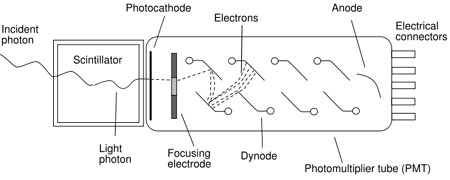
\includegraphics[width=1.0\textwidth]{figures/scintillator.jpg}
\caption{A scintillator converting an incoming photon to an electric signal.}
\label{fig:scintillator}
\end{figure}

The HB covers a pseudorapidity range of $|\eta| < 1.3$. The HE covers the range of $1.3 < |\eta| < 3$. The HE is also made of an alternating brass absorber and plastic scintillator. The HE covers 10 $\lambda_I$.

The solenoid also acts as an absorber with an interaction length of $1.4/\sin{\theta}$. Any hadrons that still have not been completely absorbed will then enter the outer HCAL (HO). With the HO, HB, and HE, the HCAL has a total absorption of 11.8 $\lambda_I$, with drops in efficiency only where the borders of the subdetectors meet.

The HF is made entirely of steel absorber with no scintillator between The HF is a thickness of 165 cm which corresponds to 10 $\lambda_I$ in steel. Electrons and photons will be absorbed within the first.
The Large Hadron Collider (LHC) beam energy, originally at 7 TeV, now for Run 3 at 13.6 TeV, allows us to study physics at the highest energy scale in history. The collaboration also performs studies of heavy ions at 30x the energy of previous heavy ion experiments. With a luminosity for pp collisions 100x greater than previous experiments, and pp cross section of about 100 mb, measurements can be done to greater precision than ever before, and searches can probe the highest ever possible masses at the TeV scale.

The LHC contains multiple experiments. At opposite points of the collider, 27 km apart, sit the A ToroidaL ApparatuS (ATLAS) and Compact Muon Solenoid (CMS) experiments. The experiments perform similar searches and measurements without sharing preliminary results. This ensures a mitigation of biases from persons performing the analyses.

The CMS experiment has 5 layers. From innermost to outermost layer sits the tracker, the electromagnetic calorimeter, the hadronic calorimeter, the solenoid, and the muon chambers. The solenoid has a 4T magnetic field. It is 13 meters long with a 6 meter inner diameter. To keep the solenoid compact, the coil is wound 4 times over to generate the 4T magnetic field. The 4T field requires a large return yoke, and so 6 endcaps and 5 barrel wheels, weighing up to 1920 tons, make up the yoke. In order to slide the solenoid in and out of the detector, the solenoid is placed on a system of air pads and grease pads that can slide the solenoid a total of 11 meters into or out of the detector. The process of sliding the solenoid 11 meters takes 1 hour to complete.

The superconducting solenoid needs to be cooled to temperatures between 4.5K and 80K. To do this, liquid helium is used and the solenoid is insulated with a 40 m$^3$ vacuum chamber. The solenoid is built to withstand a misalignment up to 10 mm between the coils and the return yoke.

The CMS solenoid is 13m long with a 6m bore diameter. The tracker, ECAL, and HCAL are situated within the bore. Due to the number of turns needed to generate a 4T magnetic field, and due to the compact nature of CMS, the solenoid is wound in 4 layers.


\vspace{-3pt}
\section{The Muon Detector System}\label{sec:ch3:muon}

\begin{figure}[h]
\centering
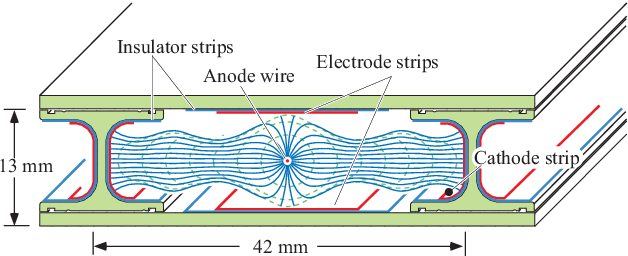
\includegraphics[width=0.75\textwidth]{figures/muon_DT_schematic.png}
\caption{Schematic of a muon detector drift tube~\cite{drift_tube_image}.}
\label{fig:muon_DT_schematic}
\end{figure}


The muon detector system is what gives the Compact Muon Solenoid detector its name. Muons are one of the most difficult standard model particles to detect, as their radiation lengths are often much longer than the length of a detector. In addition to the difficulty of detecting muons originating from collision events (called "prompt" muons), cosmic ray muons originating from our sun bombard the earth at very high rates. A muon detector system must then be very sensitive to muons while being highly shielded from cosmic rays. While some particles that are not muons may make it through the 16 $\lambda_I$ of the Tracker, ECAL, HCAL, and solenoid, the rate is so low that these hits in the muon detector are considered negligible.

Since muons experience little radiative loss in the detector, their 4-momentum can be reconstructed with high accuracy. At low momenta of $p_T < 200$ GeV, the momentum resolution is 9\%. For $p_T 1000$ GeV, the momentum resolution increases to 40\%. Together, the barrel and endcaps can trigger on the $p_T$ of muons without any extra information from the other detectors. At the Level 1 trigger, the resolution of the muons is 15-25\%.

 The barrel of the muon detector system is made of drift tube cells with 2 parallel electrode strips with a gold plate anode wire through the center of the cell also parallel to the electrode plates. A schematic of a muon drift tube is shown in Figure~\ref{fig:muon_DT_schematic}. The drift tube is filled with an AR-CO$_2$ gas mixture that provides a gain of $10^5$. 
 
 The drift tubes are staggered with an offset of 1/2 the length of a drift tube cell The staggering also helps with the detection of background hits that do not correspond to a detected track. The staggering allows the paths from muons to be reconstructed using hits from different drift tube cells.

The endcaps receive a higher rate of muons. The endcaps cover the pseudorapidity range $0.9 < |\eta| < 2.4$ and are made of Cathode Strip Chambers (CSC). Since the barrel covers the range $|\eta| < 1.2$, there are no gaps in the muon detector coverage for $|\eta| < 2.4$. 






\chapter{Event Reconstruction}\label{chap:pflow}

\section{Introduction}
\label{sec:ch4:intro}




Particle flow~\cite{particleflow} is the name given to the algorithms that take information from each of the subdetectors to reconstruct complete trajectories of most particles produced in collisions. The objects that can be identified by particle flow are the photon, charged and neutral hadrons (reconstructed as jets), the muon, and the electron. Neutrinos are not detected by CMS. Particle flow is used in CMS but was developed years before for the LEP experiment at CERN~\cite{particleflow2}.

In the ECAL charged and neutral hadrons cannot be distinguished from one another. Charged and neutral hadrons leave about 25\% of their energy in the ECAL.


Particle flow combines tracks form the tracker, vertices, and energy deposits in the ECAL and HCAL, and tracks from the muon system. The hits in the ECAL and HCAL are clustered to estimate the energy and direction of the particles. Photons are reconstructed mostly from information in the ECAL, and electrons from the tracker and ECAL. 

The resolutions of the subdetectors do mot have the same coarseness. The tracker has a much finer resolution, while the ECAL and HCAL have a coarser resolution.

 \begin{figure}[h]
\centering
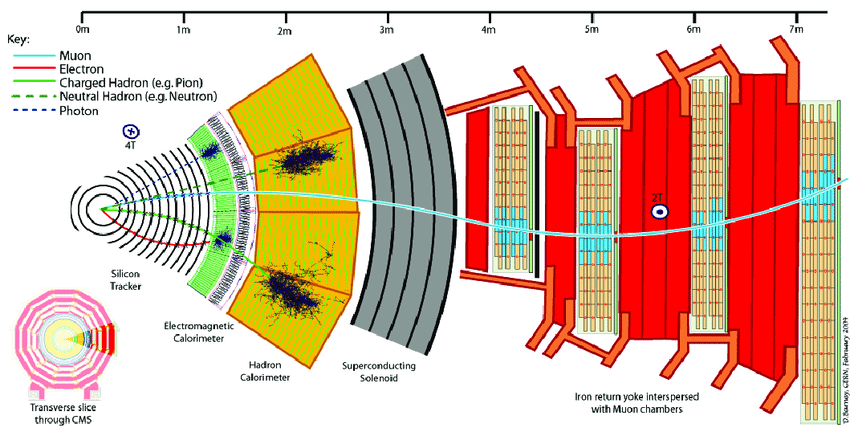
\includegraphics[width=0.9\textwidth]{figures/cms_slice}
\caption{A slice of CMS depicting the trajectory of a charged particle and its deposits in the subdetectors.}
\label{fig:cms_slice}
\end{figure}

\section{Reconstructing Charged Particles}


Charged particles are detected in the first layer of CMS, the silicone tracker. The particle tracks are reconstructed using a combinatorial track finder, which uses a randomly generated track to find the hits compatible with the detected charged-particle trajectory. 


The particle flow algorithm reconstructs tracks using iterative tracking. First, a combinatorial track finder constructs a track in 3 steps:

\begin{enumerate}
	\item Initial seed generation using hits from the tracker
	\item Collecting hits that fall within the constructed track from Step 1
	\item Final fit of the track to calculate the $p_T$ and origin of the object
\end{enumerate}




To reduce misreconstruction of tracks, this combinatorial track finding is done several times with more criteria applied each time. The hits that have already been assigned to tracks are also removed from consideration in future iterations. Some of the criteria for reconstructing a track are placed on 


\begin{itemize}
	\item $\chi^2$ of the fit
	\item track compatibility with reconstructed primary vertex
	\item track seeds
	\item track kinematics
	\item number of hits
\end{itemize}

In the first iteration, if a track with 8 hits and no more than one missing hit is found it is considered a reconstructed track and no further criteria is used. The track reconstruction algorithm goes through 10 iterations, first starting with tracks with 3 pixel hits, then on tracks with less pixel hits, then tracks with only hits in the strips, then looking for muons using information from the muon detector system.


\section{Reconstructing Neutral Hadrons}

Neutral Hadrons will deposit their energy in the HCAL but will not leave a track in the tracker, and will not deposit much energy in the ECAL.




\section{Reconstructing Electrons}

Electrons leave a track in tracker, and then when it reaches the ECAL, it deposits its energy as well as the energy of the radiating bremsstrahlung photons, which results in a supercluster in the ECAL which must be detected as coming from one electron. However this is difficult to do in practice, as energy deposits from other particles in the ECAL often overlap with the electron’s supercluster.


\section{Reconstructing Photons}

Photons appear in the detector similarly to electrons but without a track. In the ECAL, the requirements for electrons and photons are the same. A photon must be isolated from the calorimeter deposits of charged particles in the ECAL and HCAL.

\section{Reconstructing Muons}

The CMS detector is built to reconstruct muons as accurately as possible. The muon reconstruction is very efficient, with 99\% of muons accurately reconstructed. There can be false positives in the PF reconstruction of a muon, since some hadrons can punch through and be detected in the muon system. With multiple subdetectors able to identify muons, there are three ways muons are reconstructed that allows for PF reconstruction of the muon. Muons that are reconstructed in the tracker alone are called “tracker muons”. Muons that are reconstructed only in the muon detectors - the drift tubes or the cathode strip chambers - are called “standalone muons”. Muons that are reconstructed using all subdetectors are “global muons". Global muon reconstruction is the most efficient of the muon reconstructions when the muon $p_T$ is greater than 10 GeV.

In order to distinguish between muons from $q\bar{q}$ decays and muons from W and Z decays, tighter muon identification requirements are given to identify the latter events. A "soft muon" is a tracker muon with 1 pixel hit and at least 4 other inner tracker hits. The "tight muon" is a soft muon with a $\chi^2/dof < 10$, at least one hit in the muon system, and 2 matched muon segments in the muon station, the section of the muon system surrounding the solenoid.


\section{Jets}

Figure~\ref{fig:pflow_jets} shows a sketch of how the energy deposits in the ECAL and HCAL appear for the object they are associated with. Muons leave effectively no energy deposits in the calorimeters, neutral hadrons and photons leave no tracks but leave energy deposits in the HCAL and ECAL, respectively. And charged hadrons and electrons have tracks associated with their energy deposits in the calorimeters.


\begin{figure}[h]
\centering
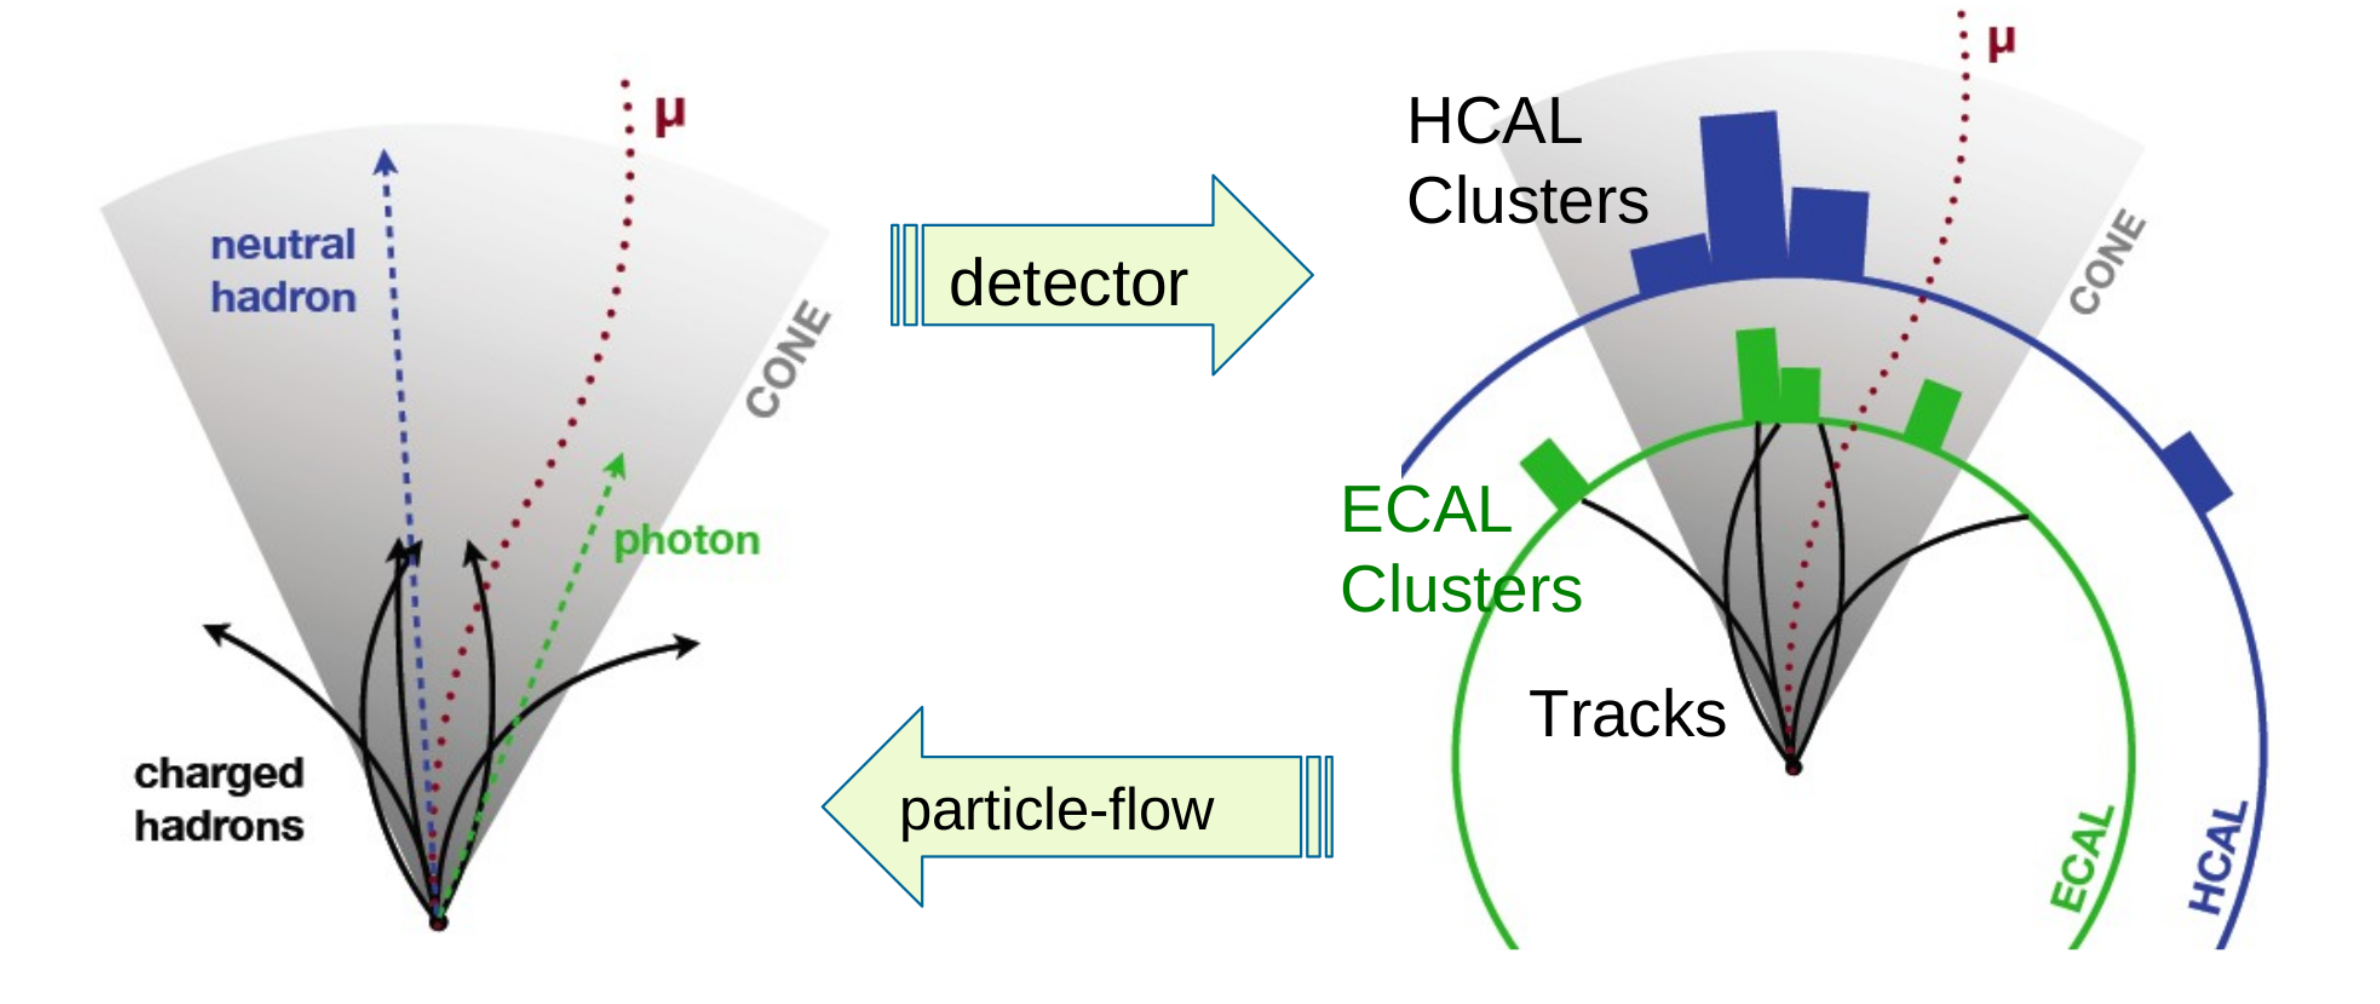
\includegraphics[width=1.0\textwidth]{figures/particle_flow_pandolfi}
\caption{A diagram of particle flow reconstruction of jets in the CMS detector~\cite{pflow_pandolfi}.}
\label{fig:pflow_jets}
\end{figure}



\subsection*{Jet Clustering}


Jets are reconstructed using a clustering algorithm. The jet clustering algorithm used in this analysis is the anti-kt algorithm. The jets clustered by the anti-kt algorithm and with a radius parameter of R=0.4 are called AK4 jets.

The anti-kt algorithm works favors clustering a particle with the nearest hard particle~\cite{anti-kt}. This ensures that soft particles are less likely to be clustered together. The algorithm for anti-kt clustering comes from the same equation used for Cambridge/Aachen clustering:

\begin{equation}
	d_{ij} = \text{min} \left( k^{2p}_{ti}, k^{2p}_{tj} \right) \frac{\Delta^2_{ij}}{R^2}
\end{equation}
\begin{equation}
	d_{iB} = k^{2p}_{ti}
\end{equation}
\begin{equation}
	\Delta_{ij}^2 = (y_i - y_j)^2 + (\phi_i - \phi_j)^2
\end{equation}

where $k_{ti}$ ($k_{tj}$) is the transverse momentum, $y_i$ ($y_j$) is the rapidity, and $\phi_i$ ($\phi_j$) is the azimuthal angle of the ith (jth) particle.

For the anti-kt algorithm, $p=-1$. Setting $p<0$ yeilds a clustering algorithm that favors jets with hard particles. The kt algorithm uses the same equations with $p=1$ and favors jest with soft radiation, and the Cambridge-Aachen algorithm uses $p=0$ which makes the algorithm $p_T$ independent.

The algorithm is performed by first calculating $d_{ij}$ and $d_{iB}$. If the minimum of the two is not $d_{iB}$, particles $i$ and $j$ are reclustered into a single particle, and the algorithm is performed again.

The AK4 jets can be reconstructed from only the ECAL and HCAL clusters. These jets are referred to as Calo Jets. The AK4 jets reconstructed with all of the particle flow information are called PF Jets. The jets reconstructed using all of the particles produced by an MC event generator are called Gen Jets. 


A diagram of these PF, Calo, and Gen jets is shown in Figure~\ref{fig:pfjet} and a graphic of particle flow reconstruction is shown in Figure~\ref{fig:pflow_jets}.


PF Jets are jets reconstructed using all particle flow candidates. PF+CHS Jets are reconstructed using all particle flow candidates except the charged hadrons associated with a pileup primary vertex. Gen Jets are jets generated from Monte Carlo simulation. Calo jets are jets made by clustering the sum of energy deposits in the ECAL and HCAL detectors.. A PF, Calo, and Ref jet for the same event are shown in the diagram for Figure~\ref{fig:pfjet}.

\begin{figure}[h]
\centering
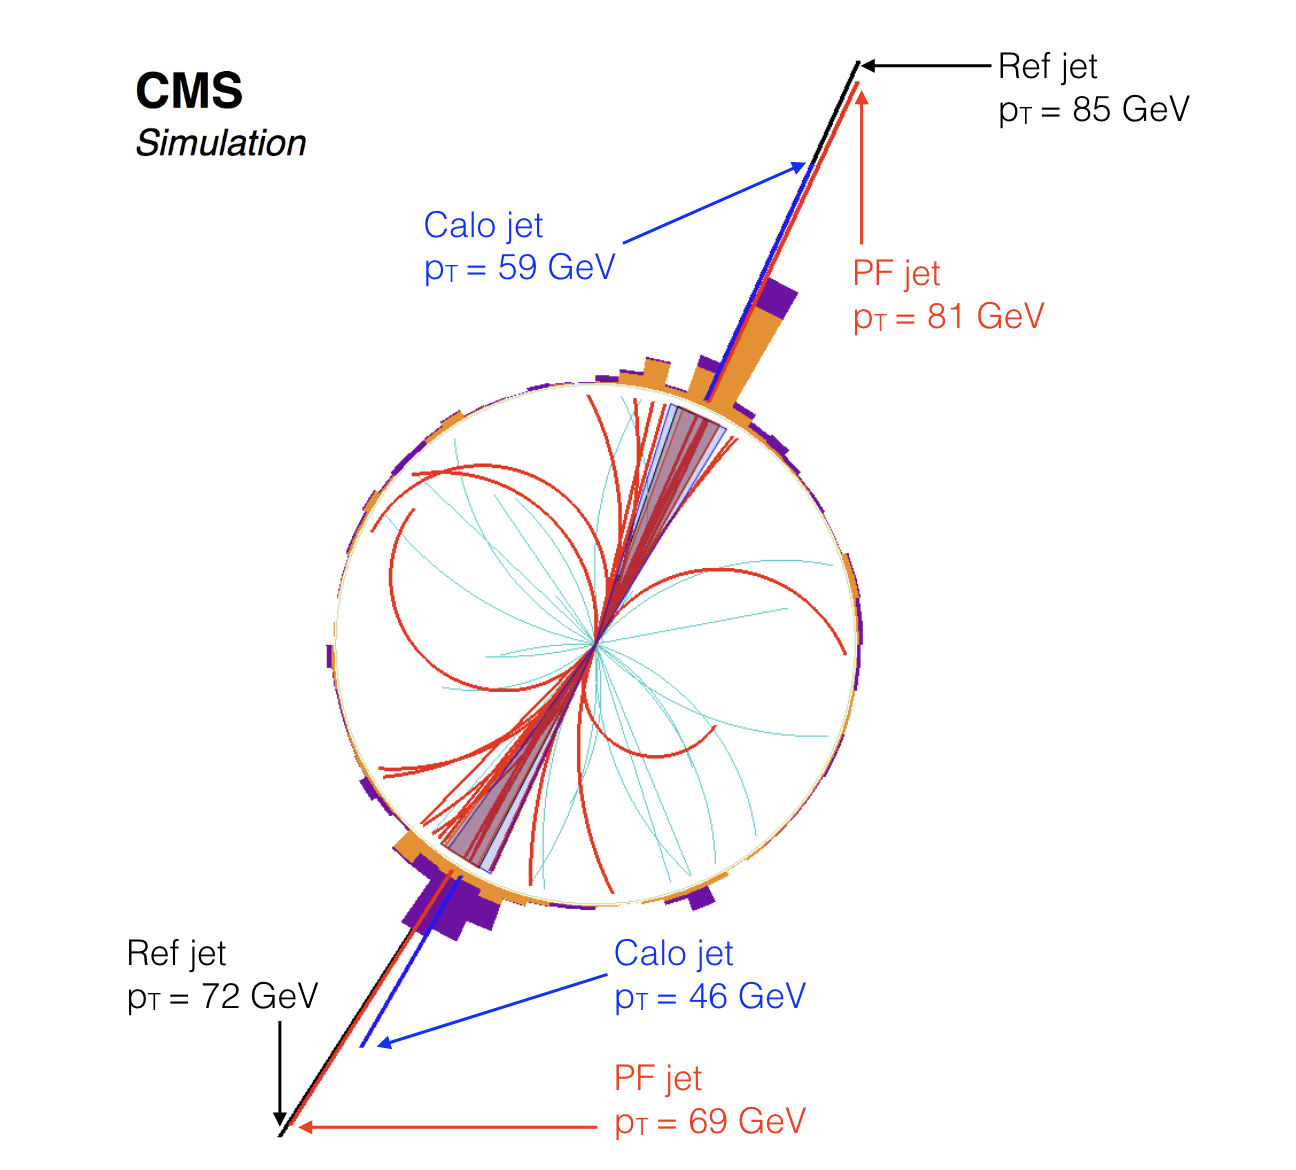
\includegraphics[width=0.9\textwidth]{figures/pf_jet_diagram}
\caption{A diagram of a dijet event and the reconstruction of the PF, Calo, and Gen (labelled as "Ref") jets~\cite{pflow}.}
\label{fig:pfjet}
\end{figure}



\subsection{Softdrop jet mass}

One of the observables in this analysis is the soft drop mass of the AK8 jets. The soft drop algorithm recursively removes soft particles which helps to distinguish boosted jets from background QCD jets. Both jets in the event are therefore required to pass the soft drop conditions~\cite{softdrop}:
	
%with a separation of $\Delta \phi > 2.1$. The semileptonic analysis requires exactly 1 top-tagged AK8 jet and hence is forced to be orthognal. Our event selection does not have dilepton events and are therefore also orthogonal to the dileptonic analysis of this channel. 

%The signal region is defined by the two jets in the ttbar candidate passing the top tagger, and by a soft drop mass window cut of $105 < m_{SD} < 210 GeV$. The sidebands of the soft drop mass are $25 < m_{SD} < 105 GeV$ and $210 < m_{SD} < 475 GeV$ and are used for background estimation. Both jets in the event are therefore required to pass the soft drop conditions:

\begin{itemize}

	\item Undo the last stage of Cambridge-Aachen clustering to to break the jet $j$ into two subjets $j_1$ and $j_2$.
	\item Require both subjets to pass the soft drop condition
	
	\begin{equation}
		   \frac {\text{min}(p_{T1},p_{T2} )}{p_{T1} + p_{T2}} >   z_{\text{cut}} \left( \frac{ \Delta R_{12} }{ R_0 } \right)^{\beta}
	\end{equation}
	
	where $p_{T1}$ and $p_{T2}$ are the $p_{T}$ of $j_1$ and $j_2$, respectively; $\Delta R_{12}$ is the distance between $j_1$ and $j_2$ in the rapidity-azimuth plane, $R_0$ is the jet radius, and $z_{\text{cut}}$ = 0.1 is the soft drop threshold, and $\beta$ = 0 is the angular exponent. 
	
	\item If the subjets pass the soft drop condition, define $j$ as the final state soft drop jet. If the subjets fail the condition, redefine the subjet with the larger $p_T$ as $j$ and iterate the soft drop algorithm.
	
\end{itemize}




\subsection*{Jet Energy Resolution and Corrections}


Reconstructed jets are calibrated using measurements from simulated QCD
 in a sequence described by the diagram in Figure~\ref{fig:jerc}. Pileup offset accounts for differences reco jets and gen jets after pileup mitigation. Jet energy resolution corrections handle the difference in jet response $R = p_{T} / p_{T,\text{gen}}$ in ($p_T$, $\eta$) bins. Jet energy scale corrections account for differences to mean jet energy resolution measurements in $\eta$ bins.

\begin{figure}[h]
\centering
	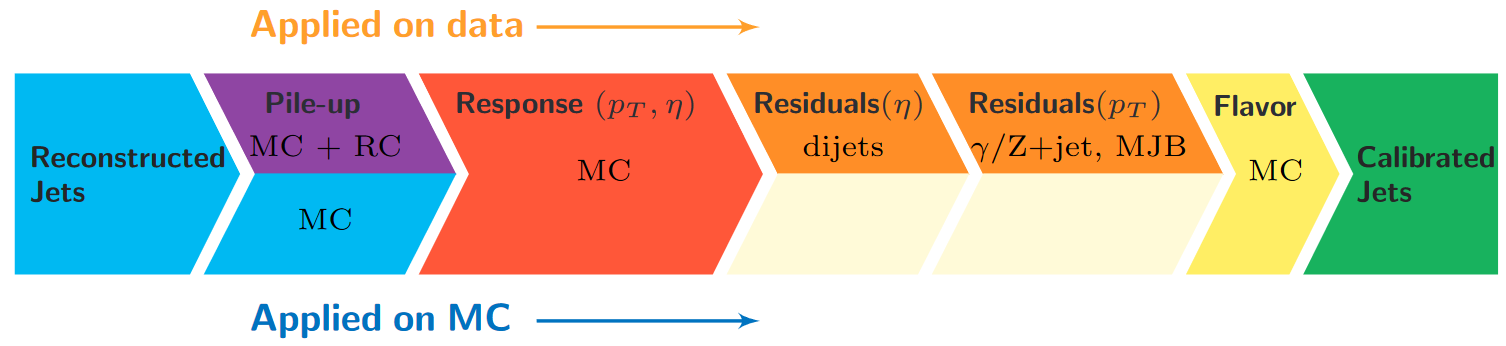
\includegraphics[width=0.8\textwidth]{figures/jerc.png}
	\caption{Diagram of the corrections applied to reconstructed jets~\cite{JEC2012}}.
	\label{fig:jerc}
\end{figure}


\section{Missing $p_T$}

The missing $p_T$ is useful for the identification of neutrinos which do not interact with any of the detector materials. It can also be useful to search for new particles. The sum of the $p_T$ in the azimuthal plane is 0 before an event, which means event in which $\sum p_{T} > 0$ has missing $p_T$. Missing $p_T$ is defined in Equation~\ref{eq:ptmiss} before jet energy corrections, and in Equation~\ref{eq:ptmiss_corr} after corrections.

\begin{equation}
	p^{miss}_{T}   = -\sum_{i=1}^{N_{particles}} p_{T_{i}}
	\label{eq:ptmiss}
\end{equation}

\begin{equation}
	p^{miss}_{T,PF}   = -\sum_{i=1}^{N_{particles}} p_{T_{i}} - \sum_{j=1}^{N_{PF\ jets}} (p_{T_{j,corr}} - p_{T_{j}})
	\label{eq:ptmiss_corr}
\end{equation}

\section{Pileup}

The pileup in an event can be estimated by the number of reconstructed primary vertices. The reconstruction efficiency of primary vertices is approximately 70\%. The primary vertex considered as the collision for the event is called the "hard scatter vertex" and is chosen by ordering the primary vertex by the $\sum p_{T}^2$.

The information from the reconstructed pileup vertices can be used to clean up the objects reconstructed by the PF algorithm. If a charged hadron has a primary vertex determined to be from a pileup collision, that hadron is subtracted from the reconstructed PF jets. These jets are saved separately as PF+CHS jets. Neutral hadrons can also be removed without track information by calculating the $p_T$ density in the $( \eta, \phi )$ plane using a similar algorithm to jet clustering.






\subsection*{Pileup Mitigation}

Pileup per particle identification (PUPPI)~\cite{puppi} weights the 4-momentum of particles in an event corresponding to how pileup-like they are. In order to assign these weights, a shape $\alpha_i$ is calculated and compared to the $\alpha$ distribution of charged pileup particles.

\begin{equation}
	\alpha_i = \log \sum_{j \in \text{event}} \frac{p_{Tj}}{R_{ij}} \times \Theta \left( R_{min} \leq \Delta R_{ij} \leq R_0  \right)
\end{equation}

where $\Theta$ is the Heaviside step function, $R_0$ is the cone size, and $R_{min} = 0.2$.


Charged Hadron Subtraction (CHS) removes charged hadrons associated with pileup vertices. In this analysis, AK8 jets use the PUPPI algorithm, and AK4 jets use the CHS algorithm for pileup mitigation.



\section{Top Tagging}
\label{sec:toptagging}

When a jet is boosted, the substructure can be exploited for tagging. Taggers apply criteria meant to separate signal jets from background. Machine Learning can also be applied to improve tagging abilities. In this analysis, the DeepAK8 mass decorrelated tagger is used~\cite{CMS:2020poo}. DeepAK8 is a machine learning tagger that takes a list of particle information and a list of secondary vertex information as inputs. The lists are then processed separately by 1 dimensional convolutional neural networks, then the outputs of the two separate layers are used as inputs in a fully connected layer, shown in Figure~\ref{fig:deepak8}.

Since many particle features are correlated with mass, the CNN is able to extract the mass of the jets. In some cases, a tagger needs to be independent of the mass of the jet. In this analysis, the background estimate uses the softdrop mass as an input, and so a tagger that does not bias the mass distribution is needed.

DeepAK8 has a mass decorrelated version which is developed by adding an additional mass prediction neural network. This mass prediction network calculates the accuracy of the CNN to extract the mass of the jet, and penalizes the tagger to remove the mass prediction.


\begin{figure}[h]
\centering
	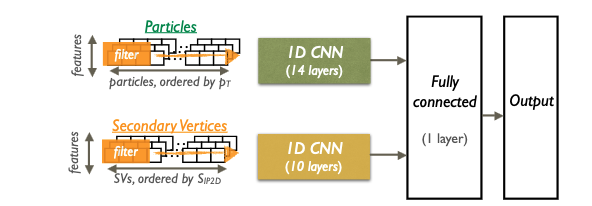
\includegraphics[width=0.8\textwidth]{figures/deepak8.png}
	\caption{Diagram of the DeepAK8 neural network.}
	\label{fig:deepak8}
\end{figure}



\chapter{$t\bar{t}$ Resonance Search}
\label{chap:analysis}


\section{Object Reconstruction}
\label{sec:reco}

This analysis selects events in which each top quark in a $t\bar{t}$ pair has decayed to a pair of quarks and a b jet that are merged into a single jet. Since the two quarks and b jet are all captured in a single boosted jet for each top quark, the jets in the event contain identifiable substructure. We utilize the standard CMS particle flow-based reconstruction of objects with the legacy Run 2 processing for data and MC. This analysis only uses jets, and hence does not select leptons or missing transverse momentum. The jet reconstruction and identification is discussed in this section.


\subsection{Jet Reconstruction}
\label{sec:jetreco}

We employ two jet collections clustered with the anti-$k_{\mathrm{T}}$ (AK) algorithm~\cite{antikt} with $R=0.4$ and $R=0.8$, reconstructed with the {\tt FASTJET} package~\cite{fastjet} referred to as ``AK4'' and ``AK8'' jets respectively. In order to mitigate the effects of pileup, "Charged Hadron Subtraction" is applied to the AK4 jets and "Pile Up Per Particle Identification'' (PUPPI) algorithm~\cite{puppi} is applied to the AK8 jets. The AK4 jet collection is used only for the construction of the $H_T$ variable, which is used to ensure the trigger efficiency is above 95\%. The rest of the analysis uses the AK8 jet collection with PUPPI. We require at least 2 top tagged AK8 jets. The jets are scaled by the Jet Energy Correction (JEC) factor~\cite{CMS:JEC} at the L1FastJet, L2Relative, L3Absolute levels. In data, an additional L2L3residual correction is applied to the jets. Since in our analysis we use both AK4 jets and AK8 jets, the corrections are applied to the AK4 and AK8 jets separately. The versions of the corrections applied are described in Table~\ref{tab:jerc}.


\begin{table}[!h]
	\centering
	\begin{tabular}{|ccc|} \hline
		Year       &  Jet Energy Corrections  &  Jet Energy Resolution   \\ \hline
		2016    &  Summer19UL16APV\_V7     &  Summer20UL16APV\_JRV3      \\
		&  Summer19UL16\_V7        &  Summer20UL16\_JRV3      \\
		2017         &  Summer19UL17\_V5        &  Summer19UL17\_JRV2   \\
		2018         &  Summer19UL18\_V5        &  Summer19UL18\_JRV2   \\\hline
	\end{tabular}
	\caption{JEC and JER versions used for each year in this analysis.}
	\label{tab:jerc}
\end{table}


\subsection{Top Quark Identification}

% I see deepAK8 but I don't see deepAK8 mass decorrelated , what it is ??? WE NEED A DISCUSSION ON THAT. 

In choosing the top tagger for this analysis, we compared ParticleNet, DeepAK8, HOTVR \cite{HOTVR}, and the CMS Top Tagger v2 (CMSv2). CMSv2 is a cut-based tagger based on an nsubjettiness cut combined with a soft drop mass window cut, $\tau_{32} < 0.65$ and $105 GeV < m_{SD} < 210 GeV$. The DeepAK8 tagger was determined to be the optimal tagger for this analysis, as it has better performance than the previously used CMSv2 tagger and is also used in the semileptonic channel of this $t\bar{t}$ analysis. Since this analysis relies heavily on a well-understood background estimate utilizing extrapolations of sidebands, we utilize the version of the tagger that has used mass decorrelation. This is a critical feature for the background estimate. 

The DeepAK8 tagger is a deep neural network (DNN) that classifies the signal of a heavy resonance decay from QCD background. The DNN takes the kinematic information of PF candidates as input variables, as well as secondary vertex and charged particle track information. The base version of DeepAK8 is correlated with the jet mass, which results in mass sculpting of background events. For our analysis we need a tagger that is mass decorrelated, as the background estimate is dependent on the jet mass. DeepAK8 has a mass decorrelated version (DeepAK8MD) that uses adversarial training to regulate the behavior of the tagger. We use the TvsQCD classification of the DeepAK8MD tagger, which distinguishes jets from top quark decays from other hadronic jets.  



% This is done for the deepAK8 mass decorrelated. The plots with the shape difference in different tagger intervals indicates a corrleation at low tagger score. Not sure if this discussion should be here. I think it should be in the background estimation study.

%Figures \ref{fig:2Ddeepak8} - \ref{fig:deepak8Windows2} shows DeepAK8's relation to the jet mass and $p_T$, demonstrating the usefulness of the tagger to pick out tops from QCD background.  Placing a cut close to a discriminator value of 1 gives a tighter selection on top events.  Values within a range of $[0.0,\ 0.2)$ gives distributions that are not always consistent with the other ranges, which can be seen in Figures \ref{fig:deepak8Windows1} and \ref{fig:deepak8Windows2}.  

While ParticleNet has better top tagging efficiency, it does not have a mass decorrelated version, which is necessary for the background estimation.
%
%\begin{figure}[!htbp]
%  \begin{center}
%    \includegraphics[width=0.50\textwidth=0.2]{Plots/tagger/ROC_tagger.png}
%    \caption{ROC curves for DeepAK8, HOTVR, and CMS top tagger v2 with comparisons to the DeepAK8 2016 working points.}
%    \label{fig:roc_tagger}
%  \end{center}
%\end{figure}
%


%\subsection{b Tagger}
%
%Our b-tagger is another DNN, DeepCSV, that was trained to discriminate between jets, both AK4 and subjets, that originate from b quark decay vs lighter quarks. For b-tagging, we check the subjets of both AK8 jets.  Therefore, we place a further requirement on the pair of AK8 jets to have 2 subjets (i.e. a successful completion of the soft drop algorithm).  An AK8 jet is considered to be b-tagged if at least one of its subjets pass the tagger cut \cite{BTVwiki}:
%
%\begin{itemize}
%\item {\bf 2016APV:} {\tt DeepCSV} $>\ 0.6001$
%\item {\bf 2016:} {\tt DeepCSV} $>\ 0.5847$
%\item {\bf 2017:} {\tt DeepCSV} $>\ 0.4506$
%\item {\bf 2018:} {\tt DeepCSV} $>\ 0.4506$  
%\end{itemize}
%
%\clearpage

\section{Event Selection Summary}

% You need the distribution of the reconstructed signal observables such as delta phi , HT, you can also show the reconstructed mass of the Heavy particles i.e  $Z^{'}$ $m_{TTbar}$}

We apply a preselection on the $p_T$, rapidity ($y$), $|\Delta \phi|$ between the two ttbar candidate AK8 jets. We use rapidity instead of pseudorapidity because the AK8 jets produced by top quarks are massive. The distribution of $H_T$ before the preselection and the distribution of $p_T$ of the leading AK8 jet of SM TTBar and 2 TeV RSGluon datasets are shown in Figures~\ref{fig:kin2016}-~\ref{fig:kin2018}.


\begin{figure}[htp]
	\begin{center}
		\includegraphics[width=0.45\textwidth]{Plots/kinematics/2016all/jetpt_inclusive.pdf}
		\includegraphics[width=0.45\textwidth]{Plots/kinematics/2016all/jetphi_inclusive.pdf}
		\includegraphics[width=0.45\textwidth]{Plots/kinematics/2016all/jeteta_inclusive.pdf}
		\includegraphics[width=0.45\textwidth]{Plots/kinematics/2016all/jety_inclusive.pdf}
		
		\caption{$p_T$, $\phi$, and  $\eta$ of the leading AK8 jet for the 2016 SM TTbar and 2 TeV RSGluon datasets.}
		\label{fig:kin2016}
	\end{center}
\end{figure}

\begin{figure}[htp]
	\begin{center}
		\includegraphics[width=0.45\textwidth]{Plots/kinematics/2017/jetpt_inclusive.pdf}
		\includegraphics[width=0.45\textwidth]{Plots/kinematics/2017/jetphi_inclusive.pdf}
		\includegraphics[width=0.45\textwidth]{Plots/kinematics/2017/jeteta_inclusive.pdf}
		\includegraphics[width=0.45\textwidth]{Plots/kinematics/2017/jety_inclusive.pdf}
		
		\caption{$p_T$, $\phi$, and  $\eta$ of the leading AK8 jet for the 2017 SM TTbar and 2 TeV RSGluon datasets.}
		\label{fig:kin2017}
	\end{center}
\end{figure}

\begin{figure}[htp]
	\begin{center}
		\includegraphics[width=0.45\textwidth]{Plots/kinematics/2018/jetpt_inclusive.pdf}
		\includegraphics[width=0.45\textwidth]{Plots/kinematics/2018/jetphi_inclusive.pdf}
		\includegraphics[width=0.45\textwidth]{Plots/kinematics/2018/jeteta_inclusive.pdf}
		\includegraphics[width=0.45\textwidth]{Plots/kinematics/2018/jety_inclusive.pdf}
		
		\caption{$p_T$, $\phi$, and  $\eta$ of the leading AK8 jet for the 2018 SM TTbar and 2 TeV RSGluon datasets.}
		\label{fig:kin2018}
	\end{center}
\end{figure}



\subsection{Kinematic Selection}


The following event selection is applied: 


\begin{itemize}
\item $\ge 2$ AK8 jets with $\pt > 400$ GeV, $|y| < 2.4$, $|\eta| < 2.4$, and loose jet ID (jetID $>$ 0 \cite{jetid})
\item $|\Delta \phi| > 2.1$ between two leading AK8 jets. 
\item $H_T > 1400$ GeV (calculated with AK4 jets) with ${\mathrm{p}}^{\mathrm{AK4}}_{\mathrm{T}}$ $>$ 30 and $|\eta^{\mathrm{AK4}}|$ $<$ 3.0; $H_T\ =\ \sum_i^{\mathrm{AK4\ Jets}}{p_{Ti}}$ (the cut value was determined by the trigger efficiency, discussed in Section~\ref{sec:trigeff})

\end{itemize}


\subsection{Trigger Selection}
\label{sec:trigeff}


The data were collected with a trigger based on the total scalar sum of transverse momenta of PF jets in the event (PFHT). Substructure based triggers such as AK8PFTH800\_TrimMass50 and similar are not used in this analysis because they bias the background estimate.


\subsection{Signal Selection}
\label{sec:signal}

The signal region is then defined by the two AK8 jets passing the 0.1\% Working Point (WP) for the mass decorrelated DeepAK8 top tagger (DeepAK8MD)~\cite{DeepAK8TopTagwiki}. The 0.1\% WP corresponds to a mistag rate of 0.1\%, and the discriminator values for each year are shown in Table~\ref{tab:deepak8}. There is also a requirement for the signal region of $105 < m_t < 210$ GeV, where $m_t$ is the softdrop mass of the leading jet.

\begin{table}[h!]
	\centering
	\begin{tabular}{|| c c  ||} 
		\hline
		Year & Discriminator Cut \\ 
		\hline\hline
		2016 & 0.889  \\ 
		2017 & 0.863  \\ 
		2018 & 0.920  \\ 
		\hline
	\end{tabular}
	\caption{Discriminator values for the 0.1\% WP for the DeepAK8MD tagger.}
	\label{tab:deepak8}
\end{table}


\subsection{Event Categorization}
\label{sec:selection}


% Add discussion on delta Y as well as support figures.


In the previous analysis, the events are divided into regions based on top tags, b-tags, and a rapidity cut for better signal purity. However, the DeepAK8MD tagger is correlated with the b-tagger, so we only split the analysis into the rapidity regions, a central region ($\Delta y < 1.0$) and a forward region ($\Delta y > 1.0$). The distribution of the $\Delta Y$ between the two leading AK8 jets is shown in Figure~\ref{fig:jety}.


\begin{figure}[htp]
	\begin{center}
		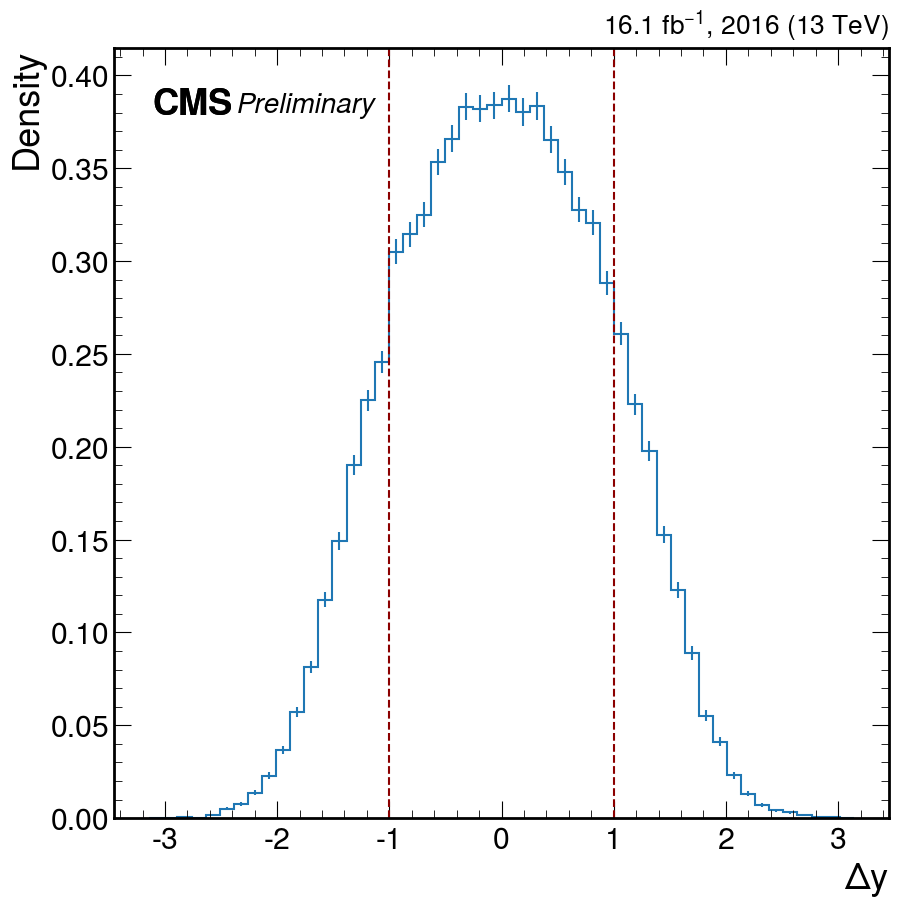
\includegraphics[width=0.3\textwidth]{Plots/kinematics/delta_rapidity.png}
		\caption{Difference in rapidity of the two AK8 jets in the $t\bar{t}$ candidate for the 2016APV datasets for the 2 TeV RSGluon.}
		\label{fig:jety}
	\end{center}
\end{figure}

\subsection{MET Filters}

We also apply the following MET filters for all UL Run II Data and MC as recommended by the JetMET POG:

\begin{itemize}
	\item {primary vertex filter}
	\item {beam halo filter}
	\item {HBHE noise filter}
	\item {HBHEiso noise filter}
	\item {ECAL TP filter}
	\item {ECAL Bad Calibration Filter}
	\item {Bad PF Muon Filter}
	\item {Bad PF Muon Dz Filter}
	\item {ee badSC noise filter}
	\item {HF noisy hits filter}
	
\end{itemize}


\subsection{Summary}


The event selection cuts and corresponding event counts in data for all years are listed in Table~\ref{tab:cutflow}.

\begin{table}
	\begin{center}
		\rowcolors{2}{gray!15}{white}
		\begin{tabular}{|p{4cm}||p{2cm}||p{2cm}||p{2cm}||p{2cm}|   } \hline 
			\textbf{Cut} & \textbf{2016 Events} & \textbf{2017 Events} & \textbf{2018 Events} & \textbf{Total Events} \\ \hline
			All Events                                 &  625,441,538  &  409,943,376 &  676,743,923  &  1,712,128,837 \\
			Trigger                                     &  77,080,857  &  37,942,480 &  44,303,284  &  159,326,621 \\
			$HT > 1400$                                 &  6,860,501  &  8,082,202 &  10,212,075  &  25,154,778 \\
			METFilter                                   &  6,800,777  &  8,024,727 &  10,159,014  &  24,984,518 \\
			AK8 JetId $>$ 1               &  6,800,639  &  8,024,617 &  10,158,742  &  24,983,998 \\
			AK8 $p_T > 400$ GeV, $|y| < 2.4$    &  6,766,299  &  7,993,862 &  10,108,968  &  24,869,129 \\
			$>=2$ AK8 Jets                               &  6,228,125  &  7,436,018 &  9,276,096  &  22,940,239 \\
			$|\Delta\varphi| > 2.1$                     &  6,154,529  &  7,344,374 &  9,170,042  &  22,668,945 \\
			\hline
		\end{tabular}
		\caption{Cutflow for JetHT events for 2016, 2017 and 2018 datasets.}
		\label{tab:cutflow}
	\end{center}
\end{table}





\subsection{HEM 15/16 Correction}

For the 2018 datasets, we take into account failures in the HCAL Endcap Minus (HEM) 15 and 16. During the last certified run of 2018B and all of 2018C and 2018D, the power supply in two HCAL modules died, impacting the jet energy measurement in this region. We apply a veto for any events with jets with $-1.57 < |\phi| < -0.87$ and $-2.5 < |\eta| < -1.3$, and jets with $-1.57 < |\phi| < -0.87$ and $-3.0< |\eta| < 2.5$. The HEM veto cuts out less than 2\% of the 2018 data.






%\section{Corrections}


%\subsection{Jet Energy Scale and Resolution}
%
%The jets are scaled by the Jet Energy Correction (JEC) factor~\cite{CMS:JEC} at the L1FastJet, L2Relative, L3Absolute levels. In data, an additional L2L3residual correction is applied to the jets. Since in our analysis we use both AK4 jets and AK8 jets, the corrections are applied to the AK4 and AK8 jets separately. The versions of the corrections applied are described in Table~\ref{tab:jerc}.
%
%
%\begin{table}[!h]
%  \centering
%  \begin{tabular}{|ccc|} \hline
%  Year       &  Jet Energy Corrections  &  Jet Energy Resolution   \\ \hline
%  2016    &  Summer19UL16APV\_V7     &  Summer20UL16APV\_JRV3      \\
%   	    &  Summer19UL16\_V7        &  Summer20UL16\_JRV3      \\
%  2017         &  Summer19UL17\_V5        &  Summer19UL17\_JRV2   \\
%  2018         &  Summer19UL18\_V5        &  Summer19UL18\_JRV2   \\\hline
%  \end{tabular}
% \caption{JEC and JER versions used for each year in this analysis.}
%\label{tab:jerc}}
%\end{table}


\subsection{Top Tagging Scale Factor}

The top tagging scale factor is implemented to account for differences in the efficiency of the top tagging in simulation and data. The scale factor is calculated as an unconstrained nuisance parameter that is extracted from the fit.


%\section{Data quality mitigation issues}

\subsection{Pileup}

The samples are generated with a different pileup distribution than the data, so they are reweighted to have a matching distribution for the number of interactions. This is done by reweighting the generated number of PU vertices in the MC to match the data, using the jsonPOG files \cite{jsonPOG}. This package is also used to propagate the uncertainty in the total inelastic cross section and is accounted for in the analysis. 


\subsection{L1 Prefiring Correction}

We take into account the effect of a timing shift in the ECAL subdetector that resulted in the Level-1 Trigger incorrectly assigning trigger flags to the previous bunch crossing. The prefiring weights depend on $p_T$ and $\eta$ and are the product of the non-firing probability of all objects in the event. We apply these corrected weights to the events of the simulated samples as suggested by ~\cite{L1prefiring}. 






\clearpage
\section{Top Tagging}
\clearpage
\section{Background Estimation}
\label{sec:bkg_est}

With an all-hadronic final state, our background is dominated by Non Top Multijet (NTMJ) events. Such events are not well modeled in simulation. Therefore we rely on a data-driven technique to accurately estimate the NTMJ background in our signal. We use the 2Dalphabet~\cite{2DAlphabet} method which relies on three variables the $m_{t}$, $m_{t\bar{t}}$ , and the mass decorelated DeepAK8 tagger score of the selected two leading jets.



%so MC QCD events do not describe the background in our signal region accurately. In order to accurately describe this dominant portion of our background, we use a data-driven background estimate, which interpolates the events counts between two sideband regions.



\subsection{2DAlphabet Method}


\begin{figure}[h!]
	\begin{center}
		\includegraphics[width=0.6\textwidth]{figures/ABCD_mtt_binc.pdf}
		\caption{The 2DAlphabet method uses sidebands in the $m_{t}$ variable and a cut on the DeepAK8MD discriminatory to separate the samples into 6 regions. The Fail ($A$,$C$,$E$) regions are then fit to the Pass ($B$,$D$,$F$) regions in the sidebands of $m_{t}$ with an analytic function $R$. The analytic function calculated in the sidebands is used to transfer the background contribution in the Fail region to the background estimate in the Pass region so that $D = RC$. The analysis is further divided into rapidity regions, and the fit is performed once for the central region and once for the forward region.}
		\label{fig:ABCD}
	\end{center}
\end{figure}



%We use the 2DAlphabet data-driven background estimate to model our NTMJ background~\cite{2DAlphabet}. 2DAlphabet 

The 2Dalphbet method is a 2D version of the simple ABCD method~\cite{ABCDmethod} and it is illustrated in Figure~\ref{fig:ABCD}. It has six regions with the signal region labeled $D$, with the requirements for each region shown in Table~\ref{tab:ABCD}.

First we compute the Fail to pass Transfer function (R) of NTMJ background, defined below, in the $m_{t}$ sidebands . Then we interpolate it from the $m_{t} $ sidebands control regions to the $m_{t}$ signal region. The background is modeled in a signal region $D$ by multiplying the control region $C$ by the transfer function, so that $C = R\times D$.


The  \textbf{Pass regions} correspond  to $B$,$D$ and $F$. An event is categorized into the Pass region if 
\begin{itemize}
	\item Both leading jets pass DeepAK8MD $>$ 0.1\% WP
\end{itemize}

The  \textbf{Fail regions} correspond to $A$,$C$,$E$. An event is categorized into the Fail region if
\begin{itemize}
	\item Leading  jet passes DeepAK8MD $>$ 0.1\% WP
	\item Sub-leading jet passes  0.5\% WP $<$ DeepAK8MD $<$  0.1\% WP
\end{itemize}


The 0.5\% WP and 0.1\% WP discriminators are shown in Table~\ref{tab:deepak8-pass-fail}.


\begin{table}[h!]
\centering
\begin{tabular}{|| c c c ||} 
 \hline
 Year & 0.5\% WP &  0.1\% WP \\ 
 \hline\hline
 2016 & 0.632 & 0.889  \\ 
 2017 & 0.554 & 0.863  \\ 
 2018 & 0.685 & 0.920  \\ 
 \hline
\end{tabular}
\caption{Discriminator values for the 0.5\% WP and 0.1\% WP for the DeepAK8MD tagger~\cite{DeepAK8TopTagwiki}.}
\label{tab:deepak8-pass-fail}
\end{table}


\begin{table}[h!]
	\centering
	\begin{tabular}{|| c || c | c | c||} 
 		 \hline
       & $25 < m_t < 105$ GeV & $105 < m_t < 210$ GeV & $210 < m_t < 475$ GeV \\ [0.5ex]  \hline\hline
		 Fail & A & C & E \\ [0.5ex] 
		 \hline 
		 Pass & B & D & F \\ [0.5ex] \hline
\end{tabular}
\caption{Requirements for the 2DAlphabet regions depicted in Figure~\ref{fig:ABCD}}.
\label{tab:ABCD}
\end{table}

The leading jets are chosen by taking the two leading $p_T$ jets after the event selection cuts. The jet with the higher DeepAK8MD discriminator of the two leading jets is the leading jet.

The NTMJ background in the Fail region is defined as the difference between data and the simulated backgrounds. In this analysis SM TTbar is the only simulated background, so NTMJ = Data - SM TTbar in the Fail region, calculated from an $m_{t \bar{t}}$ vs $m_t$ distribution, where $m_t$ is the soft-drop mass of the leading jet, and $m_{t \bar{t}}$ is the invariant mass of the two leading jets. 


Projections of the ratio of the number of events in the pass region over the number of events in the fail region ($n_{pass}/n_{fail}$) are shown for 2016 in Figures~\ref{fig:2016cen_proj}-~-\ref{fig:2016fwd_proj}. The central projection of $m_t$ is fit with a constant function, while the central $m_t$ and central and forward $m_{t\bar{t}}$ projections are fit with linear functions. The fits are not meant to be exactly the same as 2DAlphabet, but are a cross check of the choice of transfer function. The projection plots for all years can be found in Appendix~\ref{sec:appendix_2dalphabet}. The prefit Fail NTMJ distributions calculated from Data - SM TTbar are shown in Figures~\ref{fig:prefit_closure_2016}~-~\ref{fig:prefit_closure_2018}. These distributions will be multiplied by the transfer fucntion to get the Pass region NTMJ background estimate. Plots of the projections with the trends that the transfer functions are fitting are shown in Appendix~\ref{sec:appendix_2dalphabet}.


The transfer function $R$ is then initiated with all parameters = 0.1 and fit in the sideband regions of $m_t$ ($A$, $B$, $E$, $F$). After the transfer function is fit, the signal region NTMJ background estimate is calculated to be $D = R C$. The results of the background estimate in the sideband regions are shown in Figures~\ref{fig:closure_2016}~-~\ref{fig:closure_2018}.


\begin{figure}[htp]
	\begin{center}
		
		\includegraphics[width=0.45\textwidth]{Plots/2dalphabet/projections/an_v4_inconsistent_binning_2016_ttbarfits_cen_limit_0x1_projx.pdf}
		\includegraphics[width=0.45\textwidth]{Plots/2dalphabet/projections/an_v4_inconsistent_binning_2016_ttbarfits_cen_limit_0x1_projy.pdf}
		\caption{2016 central projections of $m_t$ (left) and $m_{t\bar{t}}$ (right), fit with a constant function in $m_t$ and a linear function in $m_{t\bar{t}}$.}
		\label{fig:2016cen_proj}
	\end{center}
\end{figure}



\begin{figure}[htp]
	\begin{center}
		
		\includegraphics[width=0.45\textwidth]{Plots/2dalphabet/projections/an_v4_inconsistent_binning_2016_ttbarfits_fwd_limit_1x1_projx.pdf}
		\includegraphics[width=0.45\textwidth]{Plots/2dalphabet/projections/an_v4_inconsistent_binning_2016_ttbarfits_fwd_limit_1x1_projy.pdf}
		\caption{2016 forward projections of $m_t$ (left) and $m_{t\bar{t}}$ (right), fit with a linear function in $m_t$ and a linear function in $m_{t\bar{t}}$.}
		\label{fig:2016fwd_proj}
	\end{center}
\end{figure}


\begin{figure}[!htbp]
	\begin{center}
		\includegraphics[width=0.45\textwidth=0.4]{Plots/2dalphabet//QCD_cen16Fail_postfit_2D.pdf}
		\includegraphics[width=0.45\textwidth=0.4]{Plots/2dalphabet//QCD_fwd16Fail_postfit_2D.pdf}	
		
		\caption{Fail $m_{t\bar{t}}$ vs $m_t$ of the NTMJ in the 2016 central (left) and forward (right) regions.}
		\label{fig:prefit_closure_2016}
	\end{center}
\end{figure}

\begin{figure}[!htbp]
	\begin{center}
		\includegraphics[width=0.45\textwidth=0.4]{Plots/2dalphabet//QCD_cen17Fail_postfit_2D.pdf}
		\includegraphics[width=0.45\textwidth=0.4]{Plots/2dalphabet//QCD_fwd17Fail_postfit_2D.pdf}	
		
		\caption{Fail $m_{t\bar{t}}$ vs $m_t$ of the NTMJ in the 2017 central (left) and forward (right) regions.}
		\label{fig:prefit_closure_2017}
	\end{center}
\end{figure}


\begin{figure}[!htbp]
	\begin{center}
		\includegraphics[width=0.45\textwidth=0.4]{Plots/2dalphabet//QCD_cen18Fail_postfit_2D.pdf}
		\includegraphics[width=0.45\textwidth=0.4]{Plots/2dalphabet//QCD_fwd18Fail_postfit_2D.pdf}		
		\caption{Fail $m_{t\bar{t}}$ vs $m_t$ of the NTMJ in the 2018 central (left) and forward (right) regions.}
		\label{fig:prefit_closure_2018}
	\end{center}
\end{figure}





%\begin{figure}[!htbp]
%  \begin{center}
%    \includegraphics[width=0.45\textwidth=0.2]{Plots/2dalphabet/QCD_cen16Fail_projy1.pdf} 
%    \includegraphics[width=0.45\textwidth=0.2]{Plots/2dalphabet/QCD_cen16Pass_projy1.pdf} \\ 
%        \includegraphics[width=0.45\textwidth=0.2]{Plots/2dalphabet/QCD_fwd16Fail_projy1.pdf} 
%    \includegraphics[width=0.45\textwidth=0.2]{Plots/2dalphabet/QCD_fwd16Pass_projy1.pdf} 
%    \caption{The difference between Data and SM TTbar in the Fail region (left) and the Pass region (right), for the low $m_t$ sideband in 2016 datasets for the central (top) and forward (bottom) rapidity regions.}
%    \label{fig:QCD16}
%  \end{center}
%\end{figure}
%
%
%\begin{figure}[!htbp]
%  \begin{center}
%    \includegraphics[width=0.45\textwidth=0.2]{Plots/2dalphabet/QCD_cen17Fail_projy1.pdf} 
%    \includegraphics[width=0.45\textwidth=0.2]{Plots/2dalphabet/QCD_cen17Pass_projy1.pdf} \\ 
%        \includegraphics[width=0.45\textwidth=0.2]{Plots/2dalphabet/QCD_fwd17Fail_projy1.pdf} 
%    \includegraphics[width=0.45\textwidth=0.2]{Plots/2dalphabet/QCD_fwd17Pass_projy1.pdf} 
%    \caption{The difference between Data and SM TTbar in the Fail region (left) and the Pass region (right), for the low $m_t$ sideband in 2017 datasets for the central (top) and forward (bottom) rapidity regions.}
%    \label{fig:QCD17}
%  \end{center}
%\end{figure}
%
%\begin{figure}[!htbp]
%  \begin{center}
%    \includegraphics[width=0.45\textwidth=0.2]{Plots/2dalphabet/QCD_cen18Fail_projy1.pdf} 
%    \includegraphics[width=0.45\textwidth=0.2]{Plots/2dalphabet/QCD_cen18Pass_projy1.pdf} \\ 
%        \includegraphics[width=0.45\textwidth=0.2]{Plots/2dalphabet/QCD_fwd18Fail_projy1.pdf} 
%    \includegraphics[width=0.45\textwidth=0.2]{Plots/2dalphabet/QCD_fwd18Pass_projy1.pdf} 
%    \caption{The difference between Data and SM TTbar in the Fail region (left) and the Pass region (right), for the low $m_t$ sideband in 2018 datasets for the central (top) and forward (bottom) rapidity regions.}
%    \label{fig:QCD18}
%  \end{center}
%\end{figure}

%
%\vspace{10cm}
%
%\begin{figure}[!htbp]
%
%  \begin{center}
%  \begin{picture}(100,100)
%\put(0,0){\includegraphics[width=0.45\textwidth]{Plots/2dalphabet/2016/QCD_cenFail_postfit_2D.pdf}}
%\put(90,10){$m_t$ [GeV]}
%\put(10,10){$m_{t\bar{t}}$ [GeV]}
%\end{picture} 
%
%  \caption{Plot of the Fail region with which 2DAlphabet fits the transfer function.}
%    \label{fig:NTMJ_2D_Fail}
%  \end{center}
%  
%\end{figure}
%
%\vspace{10mm}
%
%
%\begin{figure}[!htbp]
%
%  \begin{center}
%  \begin{picture}(100,100)
%\put(0,0){\includegraphics[width=0.45\textwidth]{Plots/2dalphabet/2016/QCD_cenPass_postfit_2D.pdf}}
%\put(90,10){$m_t$ [GeV]}
%\put(10,10){$m_{t\bar{t}}$ [GeV]}
%\end{picture} 
%
%  \caption{Plot of the Pass region with which 2DAlphabet fits the transfer function.}
%    \label{fig:NTMJ_2D_Pass}
%  \end{center}
%  
%\end{figure}


%The transfer function from C to D (where D is the signal region) is fit simultaneously (what do you mean?}) and interpolated from the fit in the top mass window sidebands.}\\
%{ I would suggest to add the 3D cartoon to explain the method better, this cartoon at first sight is a bit confusing, it makes me think like we are counting the number of yields instead of fitting the distribution it self}.



\subsection{Fail $\rightarrow$ Pass transfer function}

When fitting the 2D transfer function, the bins in the 2D plots of the "Pass" region are freely floating parameters in the fit. The fit is done using a 2D binned likelihood fit to data as described in Equation~\ref{eq:likelihood}~\cite{CMS:2021iuw_2dalphabet}


\begin{equation}
	\centering
	- \ln \mathcal{L} (\vec{d}, \vec{\theta}) = \sum^{N_{\text{bins, Fail}}}_{i=1} \left[ n^{NTMJ}_{Fail}(i,\vec{\theta}) - d_{Fail}(i) \ln n^{NTMJ}_{Fail}(i,\vec{\theta}) \right]   \nonumber
\end{equation}
\begin{equation}
	\centering
	+\sum^{N_{\text{bins, Pass}}}_{i=1} \left[ n^{NTMJ}_{Pass}(i,\vec{\theta}) - d_{Pass}(i)   \ln n^{NTMJ}_{Pass}(i,\vec{\theta}) \right]
\label{eq:likelihood}
\end{equation}


where $n$ is the number of events in the total background estimation, $d(i)$ is the number of observed events in data for bin $i$, and $\vec{\theta}$ is the set of nuisance parameters described by the systematic uncertainties in Section~\ref{sec:syst}.


The contribution of NTMJ events in bin $i$ of the 2D $m_{t} \text{ vs } m_{t \bar{t}}$ histogram is then

\begin{equation}
	n^{NTMJ}_{Pass}(i) = n^{NTMJ}_{Fail}(i) R_{Pass/Fail} (m_{t}, m_{t \bar{t}})
\end{equation}


The  transfer function used in this analysis is defined in equation~\ref{eq:transfer} and the parameter values for the 2016 datasets are shown in Table~\ref{tab:transfer_all}.

%The scenarios we tested for the "Pass" and "Fail" regions are:
%
%\begin{itemize}
%
%\item Medium to Antitag
%\begin{itemize}
%\item Fail: 0.2 $<$ DeepAK8MD discriminator $<$ 0.5\% WP
%\item Pass: DeepAK8MD discriminator $>$ 0.5\% WP
%\end{itemize}
%
%\item Tight to Medium
%\begin{itemize}
%\item Fail: 0.5\% WP $<$ DeepAK8MD discriminator $<$ 0.1\% WP
%\item Pass: DeepAK8MD discriminator $>$ 0.1\% WP
%\end{itemize}
%
%\end{itemize}


%The analysis is already divided into b-tag and rapidity regions (central 0b, central 1b, central 2b, forward 0b, forward 1b, forward 2b), so we tested scenarios in which either the 6 b-tag regions or 2 rapidity regions inclusive in b-tagging were fit separately using 2DAlphabet:
%
%\begin{itemize}
%\item Inclusive in btag and rapidity regions
%\item Inclusive in btag regions
%\item Split into central 0b, central 1b, central 2b, forward 0b, forward 1b, forward 2b regions
%\end{itemize}
%

%We compared the limits and determined that the "Tight to Medium" Pass to Fail, inclusive in b-tagging scenario gives the best limits for this analysis.

The transfer functions used for the  the "Tight to Medium" corresponding to "Pass to Fail" background estimate are below, and the statistical tests done to determine these functions are shown in Section~\ref{sec:ftests}
%
%\begin{equation}
%\text{2016 central } R_{\mathtext{Pass/Fail}} = (p_{0} + p_{1} m_{t} + p_{2} m^{2}_{t} + p_{3} m^{3}_{t}) (1 + p_{4} m_{t\bar{t}}) \\
%\text{2016 forward } R_{\mathtext{Pass/Fail}} = (p_{0} + p_{1} m_{t} + p_{2} m^{2}_{t}) (1 + p_{3} m_{t\bar{t}}) \\
%\text{2017 central } R_{\mathtext{Pass/Fail}} = (p_{0} + p_{1} m_{t}) (1 + p_{4} m_{t\bar{t}}) \\
%\text{2017 forward } R_{\mathtext{Pass/Fail}} = (p_{0} + p_{1} m_{t}) (1 + p_{4} m_{t\bar{t}}) \\
%\text{2018 central } R_{\mathtext{Pass/Fail}} = (p_{0} + p_{1} m_{t}) (1 + p_{4} m_{t\bar{t}}) \\
%\text{2016 forward } R_{\mathtext{Pass/Fail}} = (p_{0} + p_{1} m_{t} + p_{2} m^{2}_{t} + p_{3} m^{3}_{t}) (1 + p_{4} m_{t\bar{t}}) \\
%
%\label{eq:transfer}
%\end{equation}

\begin{equation}
\begin{aligned}
\text{central } R_{\text{Pass/Fail}} &= (a) (1 + c_{1} m_{t\bar{t}}) \\
\text{forward } R_{\text{Pass/Fail}} &= (a + b_{1} m_{t}) (1 + c_{1} m_{t\bar{t}}) \\
\end{aligned}
\label{eq:transfer}
\end{equation}

%
%\begin{table}[!htbp]
%    \centering
%    \begin{tabular}{| c | c | c | c | c | c | c | }
%        \hline
%        \textbf{Parameter} & \textbf{2016 central}  & \textbf{2016 forward} & \textbf{2017 central}  & \textbf{2017 forward} & \textbf{2018 central}  & \textbf{2018 forward}  \\
%        \hline
%	a & $1.69 \pm 0.17$  & $1.59 \pm 0.16$  & $1.56 \pm 0.15$  & $1.48 \pm 0.13$  & $1.25 \pm 0.16$  & $1.29 \pm 0.16$ \\
%	b1 & -   & $1.29 \pm 0.4$  & -   & $1.25 \pm 0.35$  & -   & $0.87 \pm 0.42$ \\
%	c1 & $2.66 \pm 0.81$  & $0.27 \pm 0.24$  & $2.82 \pm 0.68$  & $0.54 \pm 0.21$  & $1.97 \pm 0.74$  & $0.28 \pm 0.25$ \\
%        \hline
%    \end{tabular}
%    \caption{Parameter values the transfer function for the central and forward rapidity regions for all years.}
%    \label{tab:transfer_all}
%\end{table}

\begin{table}[!htbp]
    \centering
    \small
    \begin{tabular}{| p{1.8cm} | p{1.8cm} | p{1.8cm} | p{1.8cm} | p{1.8cm} | p{1.8cm} | p{1.8cm} | }
        \hline
        \textbf{Parameter} & \textbf{2016 cen}  & \textbf{2016 fwd} & \textbf{2017 cen}  & \textbf{2017 fwd} & \textbf{2018 cen}  & \textbf{2018 fwd}  \\
        \hline
        a & $1.69 \pm 0.17$  & $1.59 \pm 0.16$  & $1.56 \pm 0.15$  & $1.48 \pm 0.13$  & $1.25 \pm 0.16$  & $1.29 \pm 0.16$ \\
        b1 & -   & $1.29 \pm 0.4$  & -   & $1.25 \pm 0.35$  & -   & $0.87 \pm 0.42$ \\
        c1 & $2.66 \pm 0.81$  & $0.27 \pm 0.24$  & $2.82 \pm 0.68$  & $0.54 \pm 0.21$  & $1.97 \pm 0.74$  & $0.28 \pm 0.25$ \\
        \hline
    \end{tabular}
    \caption{Parameter values for the transfer function in the central and forward rapidity regions for all years.}
    \label{tab:transfer_all}
\end{table}



%
%The number of expected events is 
%
%\begin{equation}
%N = \sigma_{Z'} \mathcal{B} ( Z' \rightarrow t\bar{t} \rightarrow \mathrm{hadrons}) \epsilon L
%\label{eq:expected}
%\end{equation}
%
%where $\epsilon$ is the signal acceptance and efficiency, and $L$ is the integrated luminosity.

\subsection{Sideband Regions}

To validate the background estimate, we plot the $t\bar{t}$ candidate mass in the lower sideband region of the softdrop mass of the leading $p_T$ jet, after processing the datasets with same event selection and transfer function fit. The background estimate for the low mass window and high mass window is shown in Figure~\ref{fig:closure_2016} for the 2016 datasets, Figure~\ref{fig:closure_2017} for the 2017 datasets, and Figure~\ref{fig:closure_2018} for the 2018 datasets. 




\begin{figure}[!htbp]
	\begin{center}
		\includegraphics[width=0.45\textwidth=0.4]{Plots/2dalphabet/postfit_projy0_cen16Pass_logy.pdf}
		\includegraphics[width=0.45\textwidth=0.4]{Plots/2dalphabet/postfit_projy0_fwd16Pass_logy.pdf}\\
		\includegraphics[width=0.45\textwidth=0.4]{Plots/2dalphabet/postfit_projy2_cen16Pass_logy.pdf}
		\includegraphics[width=0.45\textwidth=0.4]{Plots/2dalphabet/postfit_projy2_fwd16Pass_logy.pdf}\\

		\caption{Top(bottom) Background estimate in the low(high) $m_{t}$ top mass window on the $t\bar{t}$ resonance mass distribution for the 2016 transfer function NTMJ background estimate for central (left) and forward (right) category regions.}
		\label{fig:closure_2016}
	\end{center}
\end{figure}


\begin{figure}[!htbp]
	\begin{center}
		\includegraphics[width=0.45\textwidth=0.4]{Plots/2dalphabet/postfit_projy0_cen17Pass_logy.pdf}
		\includegraphics[width=0.45\textwidth=0.4]{Plots/2dalphabet/postfit_projy0_fwd17Pass_logy.pdf}\\
		\includegraphics[width=0.45\textwidth=0.4]{Plots/2dalphabet/postfit_projy2_cen17Pass_logy.pdf}
		\includegraphics[width=0.45\textwidth=0.4]{Plots/2dalphabet/postfit_projy2_fwd17Pass_logy.pdf}\\
		
		\caption{Top(bottom) Background estimate in the low(high) $m_{t}$ top mass window on the $t\bar{t}$ resonance mass distribution for the 2017 transfer function NTMJ background estimate for central (left) and forward (right) category regions.}
		\label{fig:closure_2017}
	\end{center}
\end{figure}


\begin{figure}[!htbp]
	\begin{center}
		\includegraphics[width=0.45\textwidth=0.4]{Plots/2dalphabet/postfit_projy0_cen18Pass_logy.pdf}
		\includegraphics[width=0.45\textwidth=0.4]{Plots/2dalphabet/postfit_projy0_fwd18Pass_logy.pdf}\\
		\includegraphics[width=0.45\textwidth=0.4]{Plots/2dalphabet/postfit_projy2_cen18Pass_logy.pdf}
		\includegraphics[width=0.45\textwidth=0.4]{Plots/2dalphabet/postfit_projy2_fwd18Pass_logy.pdf}\\
		
		\caption{Top(bottom) Background estimate in the low(high) $m_{t}$ top mass window on the $t\bar{t}$ resonance mass distribution for the 2018 transfer function NTMJ background estimate for central (left) and forward (right) category regions.}
		\label{fig:closure_2018}
	\end{center}
\end{figure}







\clearpage

\section{Systematic Uncertainties} 
\label{sec:syst}

We evaluate sources of systematic uncertainties on the SM ttbar samples and the NTMJ background estimate, which affect the normalization of event yields and the shape of the invariant mass distribution. An overview of the prior systematic uncertainties input to the fit is shown in Table~\ref{tab:syst_table}, and plots of the effect of the uncertainties on the invariant mass distributions are shown in Appendix~\ref{sec:appendix_syst}.

\begin{table}[!htbp]
    \begin{center}
        \begin{tabular}{lcc}
        Systematic Uncertainty & Value & Type \\
        \hline
            Luminosity 2016 (Uncorrelated)   & 1.0\%                 & Rate         \\
            Luminosity 2017 (Uncorrelated)          & 2.0\%                 & Rate         \\
            Luminosity 2018 (Uncorrelated)          & 1.5\%                 & Rate         \\
	   	 	Luminosity 2017 (Correlated 2017, 2018)			   & 0.6\%                 & Rate         \\
	    	Luminosity 2018 (Correlated 2017, 2018)			   & 0.2\%                 & Rate         \\
            Luminosity 2016 (Correlated 2016, 2017, 2018)		   & 0.6\%                 & Rate         \\
            Luminosity 2017 (Correlated 2016, 2017, 2018)		   & 0.9\%                 & Rate         \\
            Luminosity 2018 (Correlated 2016, 2017, 2018)		   & 2.0\%                 & Rate         \\
            $t\bar{t}$ Cross Section                          & 20\%                  & Rate         \\
	   		Top Tagging SF                                      & unconstrained & Rate \\
            JES16                     & +5.1\%/-4.8\% & Rate + Shape \\
            JES17                     & +4.8\%/-4.4\% & Rate + Shape \\
            JES18                     & +5.5\%/-4.4\% & Rate + Shape \\
            JER16                      & +0.4\%/-0.5\% & Rate + Shape \\
            JER17                      & +0.7\%/-0.8\% & Rate + Shape \\
            JER18                      & +0.6\%/-0.6\% & Rate + Shape \\
            PDF Uncertainty                               &  +0.8\%/-1.7\% & Rate + Shape \\
            Pileup Uncertainty                            & +0.7\%/-0.8\% & Rate + Shape \\
            $t\bar{t}$ $Q^2$ Uncertainty                  &+24\%/-24\% & Rate + Shape \\
            L1 Prefiring                                      & +0.6\%/-0.6\% & Rate + Shape \\
            Transfer Function p0                      & $\pm 1 \sigma$ & Rate + Shape \\
            Transfer Function p1                      & $\pm 1 \sigma$ & Rate + Shape \\
            Transfer Function p2                      & $\pm 1 \sigma$ & Rate + Shape \\
        \end{tabular}
        \caption{Summary of systematic uncertainties types for this analysis.} 
        \label{tab:syst_table}
    \end{center}
\end{table}


    



\subsection{Luminosity} 

The luminosity has corresponding normalization uncertainties of $\pm$ 1.6\%,  $\pm$ 2.3\%, $\pm$ 2.5\% for the 2016, 2017, and 2018 integrated luminosity of the Run 2 datasets. 

\subsection{Cross Section }

The $t\bar{t}$ cross section has a normalization uncertainty of and $\pm$ 20\%. The 20\% prior constraint is approximately 3 times the overall uncertainty on the cross section so will allow sufficient variation in the cross section variation in the likelihood. 


\subsection{Top Tagging SF }

The uncertainty from the the scale factor is calculated during the fit, where the top tagging SF is an unconstrained nuisance parameter that is extracted from the fit.



\subsection{$Q^2$ }
The SM TTbar has a shape uncertainty from the factorization and normalization scale ($Q^2$). The $Q^2$ uncertainties are evaluated using the envelope method, in which $\mu_R$ and $\mu_F$ are varied by factors of 2 or 0.5, which results in a shape difference in the $m_{\ttbar}$ spectrum.  The shape templates for the $Q^2$ uncertainties are shown in Appendix \ref{sec:Q2_shapes}.


%\subsection{Top Tagging} \label{section:btagunc}

%A top tagging scale factor is applied twice in the signal region for SM TTbar events, and is treated as an unconstrained nuisance parameter. The scale factor is recommended by the CMS JetMET Algorithms and Reconstruction group~\cite{topTagTwiki}.

%\subsection{Top Tagging} \label{section:btagunc}

%A top tagging scale factor is applied twice in the signal region for SM TTbar events, and is treated as an unconstrained nuisance parameter. The scale factor is recommended by the CMS JetMET Algorithms and Reconstruction group~\cite{topTagTwiki}.


\subsection{Background Estimate} \label{section:BKGunc}

The background estimate is calculated using a 2D fitting function from the 2DAlphabet package. The background estimate uncertainty is then determined by varying the parameters $\pm 1 \sigma$, with uncertainties for each parameter described in Table~\ref{tab:transfer_all}.

\subsection{Pileup} \label{sectionPUunc}

The systematic uncertainties from pileup are evaluated by varying the 4.6\% uncertainty on the $69.2$ mb minimum bias cross section up and down and reweighting the pileup distribution. The shape templates for the pileup uncertainties are shown in Appendix \ref{sec:PILEUP_shapes}.

\subsection{Parton Distribution Function (PDF)} \label{sectionPDFunc}

The uncertainties from the parton distribution function of the proton are evaluated by calculating the RMS of the NNPDF3.1 PDF weights saved in the nanoAOD files for the SM TTbar and signal datasets. The shape templates for the PDF uncertainties are shown in Appendix \ref{sec:PDF_shapes}.

\subsection{Jet Energy Scale}

The jet four-momentum is varied up and down by the jet energy scale uncertainty ~\cite{CMS:JER}. The corrections are dependent on  $p_T$ and $\eta$, and are calculated both for the AK4 jets and for the AK8 jets. The shape templates for the JES uncertainties are shown in Appendix \ref{sec:JES_shapes}. A single nuisance parameter is used for all of the jet collections and years. 

\subsection{Jet Energy Resolution}

The discrepancies in the Jet Energy Resolution in the simulated samples and data is accounted for by applying eta-dependent smearing to the jets, as recommended by ~\cite{CMS:JER}. This systematic uncertainty is applied to the AK4 jets and AK8 jets in all simulated samples, and the systematic shapes can be seen in Section \ref{sec:JER_shapes}. 



%\subsection{Background Estimation}

%The systematic uncertainties in the simulated samples correspond to +/- 1 $\sigma$ uncertainties in the parameters of the 2D transfer function (equation \ref{eq:transfer}). The background estimation uncertainty is therefore a +/- 1 $\sigma$ shape uncertainty retrieved by estimating the multijet background with the transfer function parameters adjusted up or down by 1 $\sigma$ variation.





\clearpage


\section{Results}
\label{sec:results}



The postfit $m_{t\bar{t}}$ distribution of the NTMJ background, estimated using the 2D alphabet discussed in the previous section, is presented in Figure \ref{fig:mttbar_spectrum_2016} ( \ref{fig:mttbar_spectrum_20172018}) for the years 2016 (2017 and 2018), overlaid with the expected background from the $t\bar{t}$ Standard Model. The observed data are also shown. As previously published, no excess beyond the expected background is observed.

For the year 2016, since the expected limits do not exceed the previously published results, we remain unblinded, and the full 2016 dataset is utilized in the signal region, as illustrated in Figure~\ref{fig:mttbar_spectrum_2016}.

Subsequently, for 2017 and 2018, in principle, we could use 10\% of the data in the Pass region to remain blind, but this is not feasible, as the signal region becomes very low in statistics. Therefore, we present the fit results in the Fail region (medium not tight)

t

\begin{figure}[h!]
	
	\begin{center}
	     \includegraphics[width=0.49\linewidth]{Plots/2dalphabet/postfit_projy1_cen16Pass_logy.pdf} 
	     \includegraphics[width=0.49\linewidth]{Plots/2dalphabet/postfit_projy1_fwd16Pass_logy.pdf} 
		\caption{The  $t\bar{t}$ mass spectrum in the $m_{t}$ signal region (Pass) after the NTMJ background estimate using the full 2016 dataset (Unblind) for center(forward) categories left(right). }
		\label{fig:mttbar_spectrum_2016}
	\end{center}
\end{figure}

\begin{figure}[h!]
	
	\begin{center}
		\includegraphics[width=0.49\linewidth]{Plots/2dalphabet/postfit_projy1_cen17Fail_logy.pdf} 
		\includegraphics[width=0.49\linewidth]{Plots/2dalphabet/postfit_projy1_fwd17Fail_logy.pdf} \\
		
		\includegraphics[width=0.49\linewidth]{Plots/2dalphabet/postfit_projy1_cen18Fail_logy.pdf} 
		\includegraphics[width=0.49\linewidth]{Plots/2dalphabet/postfit_projy1_fwd18Fail_logy.pdf} \\
		
		\caption{Top(bottom) The  $t\bar{t}$ mass spectrum in the $m_{t}$ signal region (Fail)  after the NTMJ background estimate using the full 2017(2018) dataset for center(forward) categories left(right). }
		\label{fig:mttbar_spectrum_20172018}
	\end{center}
\end{figure}



\subsection{Limits}


In this section we compute the expected limits on $g_{kk}$, $ Z^{'}$ and $Z_{DM}$. The Upper Limit (UL) at 95 \% Confidence Level (CL) is computed using Combine software package and  is compared with the theoretical cross-section $\sigma_{th}(m)$ at Leading Order (LO).  To exclude a given signal point, the signal strength $\mu(m)$ parameter has to satisfy  
\begin{equation}
\mu(m) = \sigma_{UL}(m) / \sigma_{th}(m) < 1
\end{equation}
    


The theoretical cross section of the $g_{kk}$ are given in table ~\ref{table:RSGluonTheoryXS} and the expected limits are shown in Figure~\ref{fig:limits_run2} with the expected mass limits shown in Table~\ref{tab:limits}.
%\begin{table}[h!]
%	\centering
%	
%	\begin{tabular}{| c c |}\hline
%			\multicolumn{2}{| c |}{\textbf{ $g_{KK}$ }} \\ \hline
%			 \textbf{Mass TeV} & \textbf{$ \sigma $ (pb)} \\ \hline
%		\hline
%		
%		1.0 & 20.05 \\
%		1.5 & 3.519 \\
%		2.0 & 0.9528 \\
%		2.5 & 0.3136 \\
%		3.0 & 0.1289 \\
%		3.5 & 0.0545 \\
%		4.0 & 0.02807 \\
%		4.5 & 0.01603 \\
%		5.0 & 0.009095 \\
%		
%		\hline
%	\end{tabular}
%	
%	\caption{Expected (theory) cross sections for $g_{kk}$ gluon signal mass points}
%	\label{table:RSGluonTheoryXS}
%\end{table}

\newcommand{\ColTitle}[1]{\multicolumn{2}{|P{4cm}|}{\bf #1}} % For use in table below
\newcommand{\ColMass}{\multicolumn{1}{|P{2cm}|}{\bf Mass $(TeV)$}}
\newcommand{\ColXS}{\multicolumn{1}{|P{2cm}|}{\bf$\sigma\ (pb)$}}


\begin{figure}[!htbp]
	\begin{center}
		\includegraphics[width=0.49\linewidth]{Plots/results/limits_combine_rsgluon_all_0424.pdf} 
		\includegraphics[width=0.49\linewidth]{Plots/results/limits_combine_zprime1_all_0424.pdf} \\ 
		\includegraphics[width=0.49\linewidth]{Plots/results/limits_combine_zprime10_all_0424.pdf} 
		\includegraphics[width=0.49\linewidth]{Plots/results/limits_combine_zprime30_all_0424.pdf} \\
		\includegraphics[width=0.49\linewidth]{Plots/results/limits_combine_zprimedm_all_0424.pdf} 


		\caption{ The expected Run 2 limits for $g_{kk}$ mass for (top left), $Z'$ mass  with 1 \% width (top right),  $Z'$ mass  with 10 \% width (middle left),  $Z'$ mass  with 30 \% width (middle right), and  Run 2 (bottom)}
		\label{fig:limits_run2}
	\end{center}
\end{figure}


\begin{table}[h]
\centering
\begin{tabular}{|c|c|}
\hline
\textbf{Signal} & \textbf{Mass [TeV]} \\ \hline
$g_{kk}$ & $4.45 \pm 0.03$ \\
$Z'$ 1\% width & $3.93 \pm 0.01$ \\
$Z'$ 10\% width & $5.20 \pm 0.02$ \\
$Z'$ 30\% width & $6.62 \pm 0.04$ \\
$Z'_{DM}$ & $3.31 \pm 0.01$ \\ \hline 
\end{tabular}
\caption{Expected Run 2 mass limits.}
\label{tab:limits}
\end{table}

% {'zprimeDM_high': [3.3076, 0.005738549625000002], 'zprime1': [3.9280999999999997, 0.0034085711910000014], 'zprimeDM': [1.4472, 0.5678441562499985], 'zprime30': [6.6171999999999995, 0.030261901290000007], 'rsgluon': [4.4510000000000005, 0.022389491999999993], 'zprime10': [5.198799999999999, 0.012516775194499999]}

\newcolumntype{P}[1]{>{\centering\arraybackslash}p{#1}}



%\begin{table}[h!]
%  \begin{center}
%  \begin{tabular}{|P{2cm}P{2cm}|P{2cm}P{2cm}|P{2cm}P{2cm}|}\hline
%    \ColTitle{$Z'\ 10\%$ Width} & \ColTitle{$Z'\ 30\%$ Width} & \ColTitle{$Z'$ DM}\\ \hline
%    \ColMass & \ColXS & \ColMass & \ColXS & \ColMass & \ColXS \\ \hline
%    1.0 & 44.8526 & 1.0 & 129.361 & 1.0 & 2.222 \\ 
%    1.5 & -- & 1.5 & -- & 1.5 & 0.387 \\ 
%    2.0 & 2.26215 & 2.0 & 7.74166 & 2.0 &  0.09428 \\ 
%    2.5 & 0.734314 & 2.5 & 2.79430 & 2.5 & 0.0279  \\ 
%    3.0 & 0.272788 & 3.0 & 1.17252 & 3.0 & 0.009327  \\ 
%    3.5 & 0.112874 & 3.5 & 0.553916 & 3.5 & 0.003507  \\ 
%    4.0 & 0.0515542 & 4.0 & 0.0288839 & 4.0 & 0.001484 \\ 
%    4.5 & 0.0259114 & 4.5 & 0.163747 & 4.5 & 0.0007087, \\ 
%    5.0 & 0.0142839 & 5.0 & 0.0995997 & 5.0 & -0.0003801\\
%            
%    \hline
%  \end{tabular}
%  \caption{Expected (theory) cross sections for the corresponding $Z'$ signal mass points}
%  \label{table:ZprimeTheoryXS}
%  \end{center}
%\end{table}

\begin{table}[h!]
  \begin{center}
  \begin{tabular}{|P{2cm}P{2cm}|P{2cm}P{2cm}|}\hline
    \ColTitle{$g_{KK}$} & \ColTitle{$Z'$ DM} 		\\ \hline
    \ColMass & \ColXS & \ColMass & \ColXS  		\\ \hline
    1.0 & 20.05 		& 1.0 & 0.3637				\\ 
    1.5 & 3.519 		& 1.5 & 0.1821				\\
    2.0 & 0.9528		& 2.0 & 0.01886			\\ 
    2.5 & 0.3136 	& 2.5 & 0.005887			\\ 
    3.0 & 0.1289 	& 3.0 & 0.002111			\\ 
    3.5 & 0.0545 	& 3.5 & 8.559$\times10^{-4}$	\\ 
    4.0 & 0.02807 	& 4.0 & 3.873$\times10^{-4}$	\\ 
    4.5 & 0.01603 	& 4.5 & 1.969$\times10^{-4}$	\\ 
    5.0 & 0.009095	& 5.0 & 1.082$\times10^{-4}$	\\
     
    \hline
  \end{tabular}
  \caption{Expected (theory) cross sections for $g_{kk}$ and $Z'_{DM}$ signal mass points~\cite{CMS:xsdb}.}
  \label{table:RSGluonTheoryXS}
  \end{center}
\end{table}

\begin{table}[h!]
  \begin{center}
  \begin{tabular}{|P{2cm}P{2cm}|P{2cm}P{2cm}|P{2cm}P{2cm}|}\hline
    \ColTitle{$Z'\ 1\%$ Width} & \ColTitle{$Z'\ 10\%$ Width} & \ColTitle{$Z'\ 30\%$ Width}\\ \hline
    \ColMass & \ColXS & \ColMass & \ColXS & \ColMass & \ColXS \\ \hline
    1.0 & 3.532  		& 1.0 & 0.3637			& 1.0 & 0.1085			\\ 
    1.2 & 1.735			& 1.2 & 0.1821			& 1.2 & 0.05567			\\
    1.4 & 0.9136		& 1.4 & 0.09676			& 1.4 & 0.03084			\\
    1.6 & 0.4943		& 1.6 & 0.05402			& 1.6 & 0.01773			\\ 
    1.8 & 0.2848		& 1.8 & 0.03152			& 1.8 & 0.01072			\\ 
    2.0 & 0.1656		& 2.0 & 0.01886			& 2.0 & 0.006683		\\ 
    2.5 & 0.04757.      & 2.5 & 0.005887		& 2.5 & 0.002336		\\ 
    3.0 & 0.01477	& 3.0 & 0.002111		& 3.0 & 9.484$\times10^{-4}$	\\ 
    3.5 & 0.005054	& 3.5 & 8.559$\times10^{-4}$	& 3.5 & 8.559$\times10^{-4}$	\\ 
    4.0 & 0.00189	& 4.0 & 3.873$\times10^{-4}$	& 4.0 & 3.873$\times10^{-4}$	\\ 
    4.5 & 0.0007732	& 4.5 & 1.969$\times10^{-4}$	& 4.5 & 1.969$\times10^{-4}$	\\ 
    5.0 & 3.217$\times10^{-5}$	& 5.0 & 1.082$\times10^{-4}$	& 5.0 & 1.082$\times10^{-4}$	\\
    6.0 & 6.06$\times10^{-5}$	& 6.0 & 4.159$\times10^{-5}$	& 6.0 & 3.302$\times10^{-5}$	\\
    7.0 & 1.154$\times10^{-5}$	& 7.0 & 1.933$\times10^{-5}$	& 7.0 & 1.676$\times10^{-5}$	\\

     
    \hline
  \end{tabular}
  \caption{Expected (theory) cross sections for the corresponding $Z'$ signal mass points~\cite{NLOtheoryCurves}.}
  \label{table:ZprimeTheoryXS}
  \end{center}
\end{table}


\clearpage

\subsection{Impact}

The significance of a nuisance parameter (NP) is determined by measuring its impact and pull.   The difference between the best fit value of the NP to its pre-fit value defines the pull and is defined in following : 
\begin{equation}
	\mathrm{pull} = \frac{\hat{\theta}-\theta}{\sigma_\theta}\,,
\end{equation}
where \(\hat{\theta}\) is the best-fit value of the NP, \(\theta\) is the initial (pre-fit) value, conventionally set to zero, and \(\sigma_\theta\) is the input uncertainty. Meanwhile, the impact of an NP on a parameter of interest (POI) is the shift in the best-fit value of the POI when the NP is fixed to $\pm 1 \sigma$ of its nominal value. A low impact indicates that the NP has a negligible effect on the POI. 

\begin{equation}
	\mathrm{impact} = \Delta \mu^{\pm}=\hat{\hat{\mu}}_{\theta \pm \sigma_{\theta}}-\hat{\mu}\,.
\end{equation}

An impact plot, as shown in Figure \ref{fig:impacts}, displays the impacts of the NPs on the POIs. The highest impacts on the results come from fit NPs, as well as the $t\bar{t}$ xsec and $q^{2}$ uncertainties.

\begin{figure}[!htbp]
	\begin{center}
		\includegraphics[width=1.0\linewidth]{Plots/results/impacts_nobins.pdf} 
		\caption{Blinded Impacts for Run 2 data taking ranked in decreasing significance.}
		\label{fig:impacts}
	\end{center}
\end{figure}

\clearpage


\clearpage


\section{Statistical Analysis}
\label{sec:stats}

In this section, the obtained NTMJ background yields from the background estimation method in the signal region are presented, and the statistical evaluation used to exclude specific signal scenarios is discussed.


\subsection{F-Tests}
\label{sec:ftests}

F-tests were performed to evaluate the best transfer function for each year and rapidity region. The F-Test compares the likelihood ratios of a higher order transfer function to a lower order transfer function. The test statistic for the F-test is

\begin{equation}
	F = \frac{ -2 \ln{(\lambda_1)(\lambda_2)}/(p_2 - p_1)}{-2 \ln{(\lambda_2)}(n - p_2)}	
\end{equation}}

where $\lambda_1$ ($\lambda_2$) is the likelihood ratio of the lower (higher) order transfer function, $p_1$ ($p_2$) is the number of parameters in the lower (higher) order transfer function, and $n$ is the number of degrees of freedom.

The linear transfer functions (1x0 and 0x0) are first compared to the constant 0x0 transfer function. The 1x1 transfer function is then compared to the 0x1 and 1x0 functions. If the p-value is low (p-value < 0.3), then the 1x1 function is chosen. Higher order transfer functions are also compared to 1x1. In some cases the 2x1 is better according to the FTest, but the uncertainties on the parameters are very large. For all years, the 1x1 function is used for the forward regions, and the 0x1 for the central regions, as listed in Table~\ref{tab:TF}. The plots of the distributions of the F-Test statistic are shown in Appendix~\ref{sec:appendix_ftests}. The transfer function comparison which yields the lowest p-value is chosen for the background estimate. The functions tested are:

$$ 0x0 = a $$
$$ 1x0 = a + b_1 m_t $$
$$ 0x1 = a + b_1 m_{t\bar{t}} $$
$$ 1x1 = (a + b_1 m_t)( 1 + c_1 m_{t\bar{t}}) $$
$$ 2x1 = (a + b_1 m_t + b_2 m_t^2)( 1 + c_1 m_{t\bar{t}}) $$
$$ 1x2 = (a + b_1 m_t)( 1 + c_1 m_{t\bar{t}} + c_2 m_{t\bar{t}}^2) $$



\begin{table}[h!]
\centering
\begin{tabular}{|| c c c ||} 
 \hline
 Year & central TF  & forward TF  \\
 \hline\hline
 2016 & 0x1 & 1x1  \\ 
 2017 & 0x1 & 1x1  \\ 
 2018 & 0x1 & 1x1  \\ 
 \hline
\end{tabular}
\caption{Transfer functions selected for each year and rapidity region.}
\label{tab:TF}
\end{table}

\clearpage


\clearpage
            
\clearpage


\clearpage




%%%%%%%%%%%%%%%%%%%%%%%%%%%%%%%%%%%%%%%%%%%%%%%%%%%%%%%%%%%%%%%
% Appendices
%
% Because of a quirk in LaTeX (see p. 48 of The LaTeX
% Companion, 2e), you cannot use \include along with
% \addtocontents if you want things to appear the proper
% sequence. Since the PSU Grad School requires
%%%%%%%%%%%%%%%%%%%%%%%%%%%%%%%%%%%%%%%%%%%%%%%%%%%%%%%%%%%%%%%
%\appendix

\renewcommand{\thesection}{\Alph{section}}
\renewcommand{\thesubsection}{\thesection.\arabic{subsection}}

\begin{appendices}

\newpage
\section{Additional Kinematics Plots}
\label{sec:appendix_kinematics}


\begin{figure}[htp]
	\begin{center}
		
		\includegraphics[width=0.3\textwidth]{Plots/kinematics/2016all/jeteta_cenPass.pdf}
		\includegraphics[width=0.3\textwidth]{Plots/kinematics/2016all/jetmass_cenPass.pdf}
		\includegraphics[width=0.3\textwidth]{Plots/kinematics/2016all/jetmsd_cenPass.pdf}
		\includegraphics[width=0.3\textwidth]{Plots/kinematics/2016all/jetphi_cenPass.pdf}
		\includegraphics[width=0.3\textwidth]{Plots/kinematics/2016all/jetpt_cenPass.pdf}
		\includegraphics[width=0.3\textwidth]{Plots/kinematics/2016all/jety_cenPass.pdf}
		
		\caption{2016 kinematics plots in the central pass region for the leading AK8 jet.}
		\label{fig:kin2016_cenpass}
	\end{center}
\end{figure}



\begin{figure}[htp]
	\begin{center}

		\includegraphics[width=0.3\textwidth]{Plots/kinematics/2016all/jeteta1_cenPass.pdf}
		\includegraphics[width=0.3\textwidth]{Plots/kinematics/2016all/jetmass1_cenPass.pdf}
		\includegraphics[width=0.3\textwidth]{Plots/kinematics/2016all/jetmsd1_cenPass.pdf}
		\includegraphics[width=0.3\textwidth]{Plots/kinematics/2016all/jetphi1_cenPass.pdf}
		\includegraphics[width=0.3\textwidth]{Plots/kinematics/2016all/jetpt1_cenPass.pdf}
		\includegraphics[width=0.3\textwidth]{Plots/kinematics/2016all/jety1_cenPass.pdf}

		\caption{2016 kinematics plots in the central pass region for the sub-leading AK8 jet.}
		\label{fig:kin2016_cenpass}
	\end{center}
\end{figure}



\begin{figure}[htp]
	\begin{center}
		
		\includegraphics[width=0.3\textwidth]{Plots/kinematics/2017/jeteta_cenPass.pdf}
		\includegraphics[width=0.3\textwidth]{Plots/kinematics/2017/jetmass_cenPass.pdf}
		\includegraphics[width=0.3\textwidth]{Plots/kinematics/2017/jetmsd_cenPass.pdf}
		\includegraphics[width=0.3\textwidth]{Plots/kinematics/2017/jetphi_cenPass.pdf}
		\includegraphics[width=0.3\textwidth]{Plots/kinematics/2017/jetpt_cenPass.pdf}
		\includegraphics[width=0.3\textwidth]{Plots/kinematics/2017/jety_cenPass.pdf}
		
		\caption{2017 kinematics plots in the central pass region for the leading AK8 jet.}
		\label{fig:kin2017_cenpass}
	\end{center}
\end{figure}



\begin{figure}[htp]
	\begin{center}

		\includegraphics[width=0.3\textwidth]{Plots/kinematics/2017/jeteta1_cenPass.pdf}
		\includegraphics[width=0.3\textwidth]{Plots/kinematics/2017/jetmass1_cenPass.pdf}
		\includegraphics[width=0.3\textwidth]{Plots/kinematics/2017/jetmsd1_cenPass.pdf}
		\includegraphics[width=0.3\textwidth]{Plots/kinematics/2017/jetphi1_cenPass.pdf}
		\includegraphics[width=0.3\textwidth]{Plots/kinematics/2017/jetpt1_cenPass.pdf}
		\includegraphics[width=0.3\textwidth]{Plots/kinematics/2017/jety1_cenPass.pdf}

		\caption{2017 kinematics plots in the central pass region for the sub-leading AK8 jet.}
		\label{fig:kin2017_cenpass1}
	\end{center}
\end{figure}



\begin{figure}[htp]
	\begin{center}
		
		\includegraphics[width=0.3\textwidth]{Plots/kinematics/2017/jeteta_cenPass.pdf}
		\includegraphics[width=0.3\textwidth]{Plots/kinematics/2017/jetmass_cenPass.pdf}
		\includegraphics[width=0.3\textwidth]{Plots/kinematics/2017/jetmsd_cenPass.pdf}
		\includegraphics[width=0.3\textwidth]{Plots/kinematics/2017/jetphi_cenPass.pdf}
		\includegraphics[width=0.3\textwidth]{Plots/kinematics/2017/jetpt_cenPass.pdf}
		\includegraphics[width=0.3\textwidth]{Plots/kinematics/2017/jety_cenPass.pdf}
		
		\caption{2018 kinematics plots in the central pass region for the leading AK8 jet.}
		\label{fig:kin2018_cenpass}
	\end{center}
\end{figure}



\begin{figure}[htp]
	\begin{center}

		\includegraphics[width=0.3\textwidth]{Plots/kinematics/2017/jeteta1_cenPass.pdf}
		\includegraphics[width=0.3\textwidth]{Plots/kinematics/2017/jetmass1_cenPass.pdf}
		\includegraphics[width=0.3\textwidth]{Plots/kinematics/2017/jetmsd1_cenPass.pdf}
		\includegraphics[width=0.3\textwidth]{Plots/kinematics/2017/jetphi1_cenPass.pdf}
		\includegraphics[width=0.3\textwidth]{Plots/kinematics/2017/jetpt1_cenPass.pdf}
		\includegraphics[width=0.3\textwidth]{Plots/kinematics/2017/jety1_cenPass.pdf}

		\caption{2018 kinematics plots in the central pass region for the sub-leading AK8 jet.}
		\label{fig:kin2018_cenpass1}
	\end{center}
\end{figure}


\begin{figure}[htp]
	\begin{center}
		
		\includegraphics[width=0.3\textwidth]{Plots/kinematics/2016all/jeteta_fwdPass.pdf}
		\includegraphics[width=0.3\textwidth]{Plots/kinematics/2016all/jetmass_fwdPass.pdf}
		\includegraphics[width=0.3\textwidth]{Plots/kinematics/2016all/jetmsd_fwdPass.pdf}
		\includegraphics[width=0.3\textwidth]{Plots/kinematics/2016all/jetphi_fwdPass.pdf}
		\includegraphics[width=0.3\textwidth]{Plots/kinematics/2016all/jetpt_fwdPass.pdf}
		\includegraphics[width=0.3\textwidth]{Plots/kinematics/2016all/jety_fwdPass.pdf}
		
		\caption{2016 kinematics plots in the forward pass region for the leading AK8 jet.}
		\label{fig:kin2016_fwdPass}
	\end{center}
\end{figure}



\begin{figure}[htp]
	\begin{center}

		\includegraphics[width=0.3\textwidth]{Plots/kinematics/2016all/jeteta1_fwdPass.pdf}
		\includegraphics[width=0.3\textwidth]{Plots/kinematics/2016all/jetmass1_fwdPass.pdf}
		\includegraphics[width=0.3\textwidth]{Plots/kinematics/2016all/jetmsd1_fwdPass.pdf}
		\includegraphics[width=0.3\textwidth]{Plots/kinematics/2016all/jetphi1_fwdPass.pdf}
		\includegraphics[width=0.3\textwidth]{Plots/kinematics/2016all/jetpt1_fwdPass.pdf}
		\includegraphics[width=0.3\textwidth]{Plots/kinematics/2016all/jety1_fwdPass.pdf}

		\caption{2016 kinematics plots in the forward pass region for the sub-leading AK8 jet.}
		\label{fig:kin2016_fwdPass}
	\end{center}
\end{figure}



\begin{figure}[htp]
	\begin{center}
		
		\includegraphics[width=0.3\textwidth]{Plots/kinematics/2017/jeteta_fwdPass.pdf}
		\includegraphics[width=0.3\textwidth]{Plots/kinematics/2017/jetmass_fwdPass.pdf}
		\includegraphics[width=0.3\textwidth]{Plots/kinematics/2017/jetmsd_fwdPass.pdf}
		\includegraphics[width=0.3\textwidth]{Plots/kinematics/2017/jetphi_fwdPass.pdf}
		\includegraphics[width=0.3\textwidth]{Plots/kinematics/2017/jetpt_fwdPass.pdf}
		\includegraphics[width=0.3\textwidth]{Plots/kinematics/2017/jety_fwdPass.pdf}
		
		\caption{2017 kinematics plots in the forward pass region for the leading AK8 jet.}
		\label{fig:kin2017_fwdPass}
	\end{center}
\end{figure}



\begin{figure}[htp]
	\begin{center}

		\includegraphics[width=0.3\textwidth]{Plots/kinematics/2017/jeteta1_fwdPass.pdf}
		\includegraphics[width=0.3\textwidth]{Plots/kinematics/2017/jetmass1_fwdPass.pdf}
		\includegraphics[width=0.3\textwidth]{Plots/kinematics/2017/jetmsd1_fwdPass.pdf}
		\includegraphics[width=0.3\textwidth]{Plots/kinematics/2017/jetphi1_fwdPass.pdf}
		\includegraphics[width=0.3\textwidth]{Plots/kinematics/2017/jetpt1_fwdPass.pdf}
		\includegraphics[width=0.3\textwidth]{Plots/kinematics/2017/jety1_fwdPass.pdf}

		\caption{2017 kinematics plots in the forward pass region for the sub-leading AK8 jet.}
		\label{fig:kin2017_fwdPass1}
	\end{center}
\end{figure}



\begin{figure}[htp]
	\begin{center}
		
		\includegraphics[width=0.3\textwidth]{Plots/kinematics/2017/jeteta_fwdPass.pdf}
		\includegraphics[width=0.3\textwidth]{Plots/kinematics/2017/jetmass_fwdPass.pdf}
		\includegraphics[width=0.3\textwidth]{Plots/kinematics/2017/jetmsd_fwdPass.pdf}
		\includegraphics[width=0.3\textwidth]{Plots/kinematics/2017/jetphi_fwdPass.pdf}
		\includegraphics[width=0.3\textwidth]{Plots/kinematics/2017/jetpt_fwdPass.pdf}
		\includegraphics[width=0.3\textwidth]{Plots/kinematics/2017/jety_fwdPass.pdf}
		
		\caption{2018 kinematics plots in the forward pass region for the leading AK8 jet.}
		\label{fig:kin2018_fwdPass}
	\end{center}
\end{figure}



\begin{figure}[htp]
	\begin{center}

		\includegraphics[width=0.3\textwidth]{Plots/kinematics/2017/jeteta1_fwdPass.pdf}
		\includegraphics[width=0.3\textwidth]{Plots/kinematics/2017/jetmass1_fwdPass.pdf}
		\includegraphics[width=0.3\textwidth]{Plots/kinematics/2017/jetmsd1_fwdPass.pdf}
		\includegraphics[width=0.3\textwidth]{Plots/kinematics/2017/jetphi1_fwdPass.pdf}
		\includegraphics[width=0.3\textwidth]{Plots/kinematics/2017/jetpt1_fwdPass.pdf}
		\includegraphics[width=0.3\textwidth]{Plots/kinematics/2017/jety1_fwdPass.pdf}

		\caption{2018 kinematics plots in the forward pass region for the sub-leading AK8 jet.}
		\label{fig:kin2018_fwdPass1}
	\end{center}
\end{figure}



\begin{figure}[htp]
	\begin{center}
		
		\includegraphics[width=0.3\textwidth]{Plots/kinematics/2016all/jeteta_cenFail.pdf}
		\includegraphics[width=0.3\textwidth]{Plots/kinematics/2016all/jetmass_cenFail.pdf}
		\includegraphics[width=0.3\textwidth]{Plots/kinematics/2016all/jetmsd_cenFail.pdf}
		\includegraphics[width=0.3\textwidth]{Plots/kinematics/2016all/jetphi_cenFail.pdf}
		\includegraphics[width=0.3\textwidth]{Plots/kinematics/2016all/jetpt_cenFail.pdf}
		\includegraphics[width=0.3\textwidth]{Plots/kinematics/2016all/jety_cenFail.pdf}
		
		\caption{2016 kinematics plots in the central fail region for the leading AK8 jet.}
		\label{fig:kin2016_cenFail}
	\end{center}
\end{figure}



\begin{figure}[htp]
	\begin{center}

		\includegraphics[width=0.3\textwidth]{Plots/kinematics/2016all/jeteta1_cenFail.pdf}
		\includegraphics[width=0.3\textwidth]{Plots/kinematics/2016all/jetmass1_cenFail.pdf}
		\includegraphics[width=0.3\textwidth]{Plots/kinematics/2016all/jetmsd1_cenFail.pdf}
		\includegraphics[width=0.3\textwidth]{Plots/kinematics/2016all/jetphi1_cenFail.pdf}
		\includegraphics[width=0.3\textwidth]{Plots/kinematics/2016all/jetpt1_cenFail.pdf}
		\includegraphics[width=0.3\textwidth]{Plots/kinematics/2016all/jety1_cenFail.pdf}

		\caption{2016 kinematics plots in the central fail region for the sub-leading AK8 jet.}
		\label{fig:kin2016_cenFail}
	\end{center}
\end{figure}



\begin{figure}[htp]
	\begin{center}
		
		\includegraphics[width=0.3\textwidth]{Plots/kinematics/2017/jeteta_cenFail.pdf}
		\includegraphics[width=0.3\textwidth]{Plots/kinematics/2017/jetmass_cenFail.pdf}
		\includegraphics[width=0.3\textwidth]{Plots/kinematics/2017/jetmsd_cenFail.pdf}
		\includegraphics[width=0.3\textwidth]{Plots/kinematics/2017/jetphi_cenFail.pdf}
		\includegraphics[width=0.3\textwidth]{Plots/kinematics/2017/jetpt_cenFail.pdf}
		\includegraphics[width=0.3\textwidth]{Plots/kinematics/2017/jety_cenFail.pdf}
		
		\caption{2017 kinematics plots in the central fail region for the leading AK8 jet.}
		\label{fig:kin2017_cenFail}
	\end{center}
\end{figure}



\begin{figure}[htp]
	\begin{center}

		\includegraphics[width=0.3\textwidth]{Plots/kinematics/2017/jeteta1_cenFail.pdf}
		\includegraphics[width=0.3\textwidth]{Plots/kinematics/2017/jetmass1_cenFail.pdf}
		\includegraphics[width=0.3\textwidth]{Plots/kinematics/2017/jetmsd1_cenFail.pdf}
		\includegraphics[width=0.3\textwidth]{Plots/kinematics/2017/jetphi1_cenFail.pdf}
		\includegraphics[width=0.3\textwidth]{Plots/kinematics/2017/jetpt1_cenFail.pdf}
		\includegraphics[width=0.3\textwidth]{Plots/kinematics/2017/jety1_cenFail.pdf}

		\caption{2017 kinematics plots in the central fail region for the sub-leading AK8 jet.}
		\label{fig:kin2017_cenFail1}
	\end{center}
\end{figure}



\begin{figure}[htp]
	\begin{center}
		
		\includegraphics[width=0.3\textwidth]{Plots/kinematics/2017/jeteta_cenFail.pdf}
		\includegraphics[width=0.3\textwidth]{Plots/kinematics/2017/jetmass_cenFail.pdf}
		\includegraphics[width=0.3\textwidth]{Plots/kinematics/2017/jetmsd_cenFail.pdf}
		\includegraphics[width=0.3\textwidth]{Plots/kinematics/2017/jetphi_cenFail.pdf}
		\includegraphics[width=0.3\textwidth]{Plots/kinematics/2017/jetpt_cenFail.pdf}
		\includegraphics[width=0.3\textwidth]{Plots/kinematics/2017/jety_cenFail.pdf}
		
		\caption{2018 kinematics plots in the central fail region for the leading AK8 jet.}
		\label{fig:kin2018_cenFail}
	\end{center}
\end{figure}



\begin{figure}[htp]
	\begin{center}

		\includegraphics[width=0.3\textwidth]{Plots/kinematics/2017/jeteta1_cenFail.pdf}
		\includegraphics[width=0.3\textwidth]{Plots/kinematics/2017/jetmass1_cenFail.pdf}
		\includegraphics[width=0.3\textwidth]{Plots/kinematics/2017/jetmsd1_cenFail.pdf}
		\includegraphics[width=0.3\textwidth]{Plots/kinematics/2017/jetphi1_cenFail.pdf}
		\includegraphics[width=0.3\textwidth]{Plots/kinematics/2017/jetpt1_cenFail.pdf}
		\includegraphics[width=0.3\textwidth]{Plots/kinematics/2017/jety1_cenFail.pdf}

		\caption{2018 kinematics plots in the central fail region for the sub-leading AK8 jet.}
		\label{fig:kin2018_cenFail1}
	\end{center}
\end{figure}


\begin{figure}[htp]
	\begin{center}
		
		\includegraphics[width=0.3\textwidth]{Plots/kinematics/2016all/jeteta_fwdFail.pdf}
		\includegraphics[width=0.3\textwidth]{Plots/kinematics/2016all/jetmass_fwdFail.pdf}
		\includegraphics[width=0.3\textwidth]{Plots/kinematics/2016all/jetmsd_fwdFail.pdf}
		\includegraphics[width=0.3\textwidth]{Plots/kinematics/2016all/jetphi_fwdFail.pdf}
		\includegraphics[width=0.3\textwidth]{Plots/kinematics/2016all/jetpt_fwdFail.pdf}
		\includegraphics[width=0.3\textwidth]{Plots/kinematics/2016all/jety_fwdFail.pdf}
		
		\caption{2016 kinematics plots in the forward fail region for the leading AK8 jet.}
		\label{fig:kin2016_fwdFail}
	\end{center}
\end{figure}



\begin{figure}[htp]
	\begin{center}

		\includegraphics[width=0.3\textwidth]{Plots/kinematics/2016all/jeteta1_fwdFail.pdf}
		\includegraphics[width=0.3\textwidth]{Plots/kinematics/2016all/jetmass1_fwdFail.pdf}
		\includegraphics[width=0.3\textwidth]{Plots/kinematics/2016all/jetmsd1_fwdFail.pdf}
		\includegraphics[width=0.3\textwidth]{Plots/kinematics/2016all/jetphi1_fwdFail.pdf}
		\includegraphics[width=0.3\textwidth]{Plots/kinematics/2016all/jetpt1_fwdFail.pdf}
		\includegraphics[width=0.3\textwidth]{Plots/kinematics/2016all/jety1_fwdFail.pdf}

		\caption{2016 kinematics plots in the forward fail region for the sub-leading AK8 jet.}
		\label{fig:kin2016_fwdFail}
	\end{center}
\end{figure}



\begin{figure}[htp]
	\begin{center}
		
		\includegraphics[width=0.3\textwidth]{Plots/kinematics/2017/jeteta_fwdFail.pdf}
		\includegraphics[width=0.3\textwidth]{Plots/kinematics/2017/jetmass_fwdFail.pdf}
		\includegraphics[width=0.3\textwidth]{Plots/kinematics/2017/jetmsd_fwdFail.pdf}
		\includegraphics[width=0.3\textwidth]{Plots/kinematics/2017/jetphi_fwdFail.pdf}
		\includegraphics[width=0.3\textwidth]{Plots/kinematics/2017/jetpt_fwdFail.pdf}
		\includegraphics[width=0.3\textwidth]{Plots/kinematics/2017/jety_fwdFail.pdf}
		
		\caption{2017 kinematics plots in the forward fail region for the leading AK8 jet.}
		\label{fig:kin2017_fwdFail}
	\end{center}
\end{figure}



\begin{figure}[htp]
	\begin{center}

		\includegraphics[width=0.3\textwidth]{Plots/kinematics/2017/jeteta1_fwdFail.pdf}
		\includegraphics[width=0.3\textwidth]{Plots/kinematics/2017/jetmass1_fwdFail.pdf}
		\includegraphics[width=0.3\textwidth]{Plots/kinematics/2017/jetmsd1_fwdFail.pdf}
		\includegraphics[width=0.3\textwidth]{Plots/kinematics/2017/jetphi1_fwdFail.pdf}
		\includegraphics[width=0.3\textwidth]{Plots/kinematics/2017/jetpt1_fwdFail.pdf}
		\includegraphics[width=0.3\textwidth]{Plots/kinematics/2017/jety1_fwdFail.pdf}

		\caption{2017 kinematics plots in the forward fail region for the sub-leading AK8 jet.}
		\label{fig:kin2017_fwdFail1}
	\end{center}
\end{figure}



\begin{figure}[htp]
	\begin{center}
		
		\includegraphics[width=0.3\textwidth]{Plots/kinematics/2017/jeteta_fwdFail.pdf}
		\includegraphics[width=0.3\textwidth]{Plots/kinematics/2017/jetmass_fwdFail.pdf}
		\includegraphics[width=0.3\textwidth]{Plots/kinematics/2017/jetmsd_fwdFail.pdf}
		\includegraphics[width=0.3\textwidth]{Plots/kinematics/2017/jetphi_fwdFail.pdf}
		\includegraphics[width=0.3\textwidth]{Plots/kinematics/2017/jetpt_fwdFail.pdf}
		\includegraphics[width=0.3\textwidth]{Plots/kinematics/2017/jety_fwdFail.pdf}
		
		\caption{2018 kinematics plots in the forward fail region for the leading AK8 jet.}
		\label{fig:kin2018_fwdFail}
	\end{center}
\end{figure}



\begin{figure}[htp]
	\begin{center}

		\includegraphics[width=0.3\textwidth]{Plots/kinematics/2017/jeteta1_fwdFail.pdf}
		\includegraphics[width=0.3\textwidth]{Plots/kinematics/2017/jetmass1_fwdFail.pdf}
		\includegraphics[width=0.3\textwidth]{Plots/kinematics/2017/jetmsd1_fwdFail.pdf}
		\includegraphics[width=0.3\textwidth]{Plots/kinematics/2017/jetphi1_fwdFail.pdf}
		\includegraphics[width=0.3\textwidth]{Plots/kinematics/2017/jetpt1_fwdFail.pdf}
		\includegraphics[width=0.3\textwidth]{Plots/kinematics/2017/jety1_fwdFail.pdf}

		\caption{2018 kinematics plots in the forward fail region for the sub-leading AK8 jet.}
		\label{fig:kin2018_fwdFail1}
	\end{center}
\end{figure}



\begin{figure}[htp]
	\begin{center}

		\includegraphics[width=0.3\textwidth]{Plots/kinematics/2016all/ht_inclusive.pdf}
		\includegraphics[width=0.3\textwidth]{Plots/kinematics/2017/ht_inclusive.pdf}
		\includegraphics[width=0.3\textwidth]{Plots/kinematics/2018/ht_inclusive.pdf}

		\caption{$H_T$ of SM TTbar and $g_{KK}$ 2 TeV signal for 2016 (left), 2017 (middle), and 2018 (right).}
		\label{fig:kin2018_fwdFail1}
	\end{center}
\end{figure}





\section{2DAlphabet Projection Plots}
\label{sec:appendix_2dalphabet}

Figures~\ref{fig:2016cen_proj}~-~\ref{fig:2018fwd_proj} show the projections in $m_t$ and $m_{\ttbar}$ of $n_{pass}/n_{fail}$ for the prefit NTMJ background in the sidebands of the 2DAlphabet background estimate (A,B,E,F) (see Table~\ref{tab:ABCD}). The projections are fit with a constant or linear function depending on whether the transfer function is constant or linear with respect to $m_t$ and $m_{\ttbar}$. The central transfer functions are 0x1 (constant with respect to $m_t$ and linear with respect to $m_{\ttbar}$), and the forward transfer functions are 1x1 (linear with respect to $m_t$ and linear with respect to $m_{\ttbar}$).

\begin{figure}[htp]
	\begin{center}
		
		\includegraphics[width=0.45\textwidth]{Plots/2dalphabet/projections/an_v4_inconsistent_binning_2016_ttbarfits_cen_limit_0x1_projx.pdf}
		\includegraphics[width=0.45\textwidth]{Plots/2dalphabet/projections/an_v4_inconsistent_binning_2016_ttbarfits_cen_limit_0x1_projy.pdf}
		\caption{2016 central projections of $m_t$ (left) and $m_{\ttbar}$ (right), fit with a constant function in $m_t$ and a linear function in $m_{\ttbar}$.}
		\label{fig:2016cen_proj}
	\end{center}
\end{figure}



\begin{figure}[htp]
	\begin{center}
		
		\includegraphics[width=0.45\textwidth]{Plots/2dalphabet/projections/an_v4_inconsistent_binning_2016_ttbarfits_fwd_limit_1x1_projx.pdf}
		\includegraphics[width=0.45\textwidth]{Plots/2dalphabet/projections/an_v4_inconsistent_binning_2016_ttbarfits_fwd_limit_1x1_projy.pdf}
		\caption{2016 forward projections of $m_t$ (left) and $m_{\ttbar}$ (right), fit with a linear function in $m_t$ and a linear function in $m_{\ttbar}$.}
		\label{fig:2016fwd_proj}
	\end{center}
\end{figure}





\begin{figure}[htp]
	\begin{center}
		
		\includegraphics[width=0.45\textwidth]{Plots/2dalphabet/projections/an_v4_inconsistent_binning_2017_ttbarfits_cen_limit_0x1_projx.pdf}
		\includegraphics[width=0.45\textwidth]{Plots/2dalphabet/projections/an_v4_inconsistent_binning_2017_ttbarfits_cen_limit_0x1_projy.pdf}
		\caption{2017 central projections of $m_t$ (left) and $m_{\ttbar}$ (right), fit with a constant function in $m_t$ and a linear function in $m_{\ttbar}$.}
		\label{fig:2017cen_proj}
	\end{center}
\end{figure}





\begin{figure}[htp]
	\begin{center}
		
		\includegraphics[width=0.45\textwidth]{Plots/2dalphabet/projections/an_v4_inconsistent_binning_2017_ttbarfits_fwd_limit_1x1_projx.pdf}
		\includegraphics[width=0.45\textwidth]{Plots/2dalphabet/projections/an_v4_inconsistent_binning_2017_ttbarfits_fwd_limit_1x1_projy.pdf}
		\caption{2017 forward projections of $m_t$ (left) and $m_{\ttbar}$ (right), fit with a linear function in $m_t$ and a linear function in $m_{\ttbar}$.}
		\label{fig:2017fwd_proj}
	\end{center}
\end{figure}




\begin{figure}[htp]
	\begin{center}
		
		\includegraphics[width=0.45\textwidth]{Plots/2dalphabet/projections/an_v4_inconsistent_binning_2018_ttbarfits_cen_limit_0x1_projx.pdf}
		\includegraphics[width=0.45\textwidth]{Plots/2dalphabet/projections/an_v4_inconsistent_binning_2018_ttbarfits_cen_limit_0x1_projy.pdf}
		\caption{2018 central projections of $m_t$ (left) and $m_{\ttbar}$ (right), fit with a constant function in $m_t$ and a linear function in $m_{\ttbar}$.}
		\label{fig:2018cen_proj}
	\end{center}
\end{figure}



\begin{figure}[htp]
	\begin{center}
		
		\includegraphics[width=0.45\textwidth]{Plots/2dalphabet/projections/an_v4_inconsistent_binning_2018_ttbarfits_fwd_limit_1x1_projx.pdf}
		\includegraphics[width=0.45\textwidth]{Plots/2dalphabet/projections/an_v4_inconsistent_binning_2018_ttbarfits_fwd_limit_1x1_projy.pdf}
		\caption{2018 forward projections of $m_t$ (left) and $m_{\ttbar}$ (right), fit with a linear function in $m_t$ and a linear function in $m_{\ttbar}$.}
		\label{fig:2018fwd_proj}
	\end{center}
\end{figure}

\newpage
\section{Systematic Shape Templates}
\label{sec:appendix_syst}

In the following section we provide the  $\pm 1\sigma$ shape uncertainties for the MC samples.
\vspace{-2mm}

\subsection{JES Uncertainty}
 \label{sec:JES_shapes}
 
\vspace{-2mm}

\subsubsection*{SM TTbar}

\vspace{-2mm}

\begin{figure}[!htbp]
\begin{center}
\includegraphics[width=0.4\linewidth]{Plots/systematics/2016/TTbar_cen_jes.pdf}
\includegraphics[width=0.4\linewidth]{Plots/systematics/2016/TTbar_fwd_jes.pdf} \\
\includegraphics[width=0.4\linewidth]{Plots/systematics/2017/TTbar_cen_jes.pdf}
\includegraphics[width=0.4\linewidth]{Plots/systematics/2017/TTbar_fwd_jes.pdf} \\
\includegraphics[width=0.4\linewidth]{Plots/systematics/2018/TTbar_cen_jes.pdf}
\includegraphics[width=0.4\linewidth]{Plots/systematics/2018/TTbar_fwd_jes.pdf} \\
\caption{Effect of the jes uncertainties on the $m_{\ttbar}$ shape for the $t\bar{t}$ Monte Carlo sample for the central and forward analysis categories for 2016, 2017, and 2018 datasets.}
\label{fig:syst_jes_tt}
\end{center}
\end{figure}



\newpage






\subsection{JER Uncertainty}
 \label{sec:JER_shapes}
 
 
\subsubsection*{SM TTbar}

\begin{figure}[!htbp]
\begin{center}
\includegraphics[width=0.4\linewidth]{Plots/systematics/2016/TTbar_cen_jer.pdf}
\includegraphics[width=0.4\linewidth]{Plots/systematics/2016/TTbar_fwd_jer.pdf} \\
\includegraphics[width=0.4\linewidth]{Plots/systematics/2017/TTbar_cen_jer.pdf}
\includegraphics[width=0.4\linewidth]{Plots/systematics/2017/TTbar_fwd_jer.pdf} \\
\includegraphics[width=0.4\linewidth]{Plots/systematics/2018/TTbar_cen_jer.pdf}
\includegraphics[width=0.4\linewidth]{Plots/systematics/2018/TTbar_fwd_jer.pdf} \\
\caption{Effect of the jer uncertainties on the $m_{\ttbar}$ shape for the $t\bar{t}$ Monte Carlo sample for the central and forward analysis categories for 2016, 2017, and 2018 datasets.}
\label{fig:syst_jer_tt}
\end{center}
\end{figure}

\newpage



\subsection{Pileup Uncertainty}
 \label{sec:PILEUP_shapes}
 
 
\subsubsection*{SM TTbar}

\begin{figure}[!htbp]
\begin{center}
\includegraphics[width=0.4\linewidth]{Plots/systematics/2016/TTbar_cen_pileup.pdf}
\includegraphics[width=0.4\linewidth]{Plots/systematics/2016/TTbar_fwd_pileup.pdf} \\
\includegraphics[width=0.4\linewidth]{Plots/systematics/2017/TTbar_cen_pileup.pdf}
\includegraphics[width=0.4\linewidth]{Plots/systematics/2017/TTbar_fwd_pileup.pdf} \\
\includegraphics[width=0.4\linewidth]{Plots/systematics/2018/TTbar_cen_pileup.pdf}
\includegraphics[width=0.4\linewidth]{Plots/systematics/2018/TTbar_fwd_pileup.pdf} \\
\caption{Effect of the pileup uncertainties on the $m_{\ttbar}$ shape for the $t\bar{t}$ Monte Carlo sample for the central and forward analysis categories for 2016, 2017, and 2018 datasets.}
\label{fig:syst_pileup_tt}
\end{center}
\end{figure}

\newpage



\subsection{PDF Uncertainty}
 \label{sec:PDF_shapes}
 
 
\subsubsection*{SM TTbar}

\begin{figure}[!htbp]
\begin{center}
\includegraphics[width=0.4\linewidth]{Plots/systematics/2016/TTbar_cen_pdf.pdf}
\includegraphics[width=0.4\linewidth]{Plots/systematics/2016/TTbar_fwd_pdf.pdf} \\
\includegraphics[width=0.4\linewidth]{Plots/systematics/2017/TTbar_cen_pdf.pdf}
\includegraphics[width=0.4\linewidth]{Plots/systematics/2017/TTbar_fwd_pdf.pdf} \\
\includegraphics[width=0.4\linewidth]{Plots/systematics/2018/TTbar_cen_pdf.pdf}
\includegraphics[width=0.4\linewidth]{Plots/systematics/2018/TTbar_fwd_pdf.pdf} \\
\caption{Effect of the pdf uncertainties on the $m_{\ttbar}$ shape for the $t\bar{t}$ Monte Carlo sample at the 2 TeV mass point for the central and forward analysis categories for 2016, 2017, and 2018 datasets.}
\label{fig:syst_pdf_rs5}
\end{center}
\end{figure}

\newpage




\subsection{Q2 Uncertainty}
 \label{sec:Q2_shapes}
 
 
\subsubsection*{SM TTbar}

\begin{figure}[!htbp]
\begin{center}
\includegraphics[width=0.4\linewidth]{Plots/systematics/2016/TTbar_cen_q2.pdf}
\includegraphics[width=0.4\linewidth]{Plots/systematics/2016/TTbar_fwd_q2.pdf} \\
\includegraphics[width=0.4\linewidth]{Plots/systematics/2017/TTbar_cen_q2.pdf}
\includegraphics[width=0.4\linewidth]{Plots/systematics/2017/TTbar_fwd_q2.pdf} \\
\includegraphics[width=0.4\linewidth]{Plots/systematics/2018/TTbar_cen_q2.pdf}
\includegraphics[width=0.4\linewidth]{Plots/systematics/2018/TTbar_fwd_q2.pdf} \\
\caption{Effect of the q2 uncertainties on the $m_{\ttbar}$ shape for the $t\bar{t}$ Monte Carlo sample for the central and forward analysis categories for 2016, 2017, and 2018 datasets.}
\label{fig:syst_q2_tt}
\end{center}
\end{figure}

\newpage


\subsection{Prefiring Uncertainty}
 \label{sec:PREFIRING_shapes}
 
 
\subsubsection*{SM TTbar}

\begin{figure}[!htbp]
\begin{center}
\includegraphics[width=0.4\linewidth]{Plots/systematics/2016/TTbar_cen_prefiring.pdf}
\includegraphics[width=0.4\linewidth]{Plots/systematics/2016/TTbar_fwd_prefiring.pdf} \\
\includegraphics[width=0.4\linewidth]{Plots/systematics/2017/TTbar_cen_prefiring.pdf}
\includegraphics[width=0.4\linewidth]{Plots/systematics/2017/TTbar_fwd_prefiring.pdf} \\
\caption{Effect of the prefiring uncertainties on the $m_{\ttbar}$ shape for the $t\bar{t}$ Monte Carlo sample for the central and forward analysis categories for 2016 and 2017 datasets.}
\label{fig:syst_prefiring_tt}
\end{center}
\end{figure}

\newpage


\newpage
\section{Limits}
\label{sec:appendix_limits}



\begin{figure}[!htbp]
	\begin{center}
		\includegraphics[width=0.49\linewidth]{Plots/results/limits_combine_rsgluon_2016_0424.pdf} 
		\includegraphics[width=0.49\linewidth]{Plots/results/limits_combine_rsgluon_2017_0424.pdf} \\
		\includegraphics[width=0.49\linewidth]{Plots/results/limits_combine_rsgluon_2018_0424.pdf}
		\includegraphics[width=0.49\linewidth]{Plots/results/limits_combine_rsgluon_all_0424.pdf} 
		
		\caption{ The expected limits on $g_{kk}$ mass for 2016 (top left),  2017 (top right),  2018 (bottom left), and  Run 2 (bottom right)}
		\label{fig:limits_on_RS_gluons}
	\end{center}
\end{figure}

\begin{figure}[!htbp]
	\begin{center}
		\includegraphics[width=0.49\linewidth]{Plots/results/limits_combine_zprimedm_2016_0424.pdf} 
		\includegraphics[width=0.49\linewidth]{Plots/results/limits_combine_zprimedm_2017_0424.pdf} \\
		\includegraphics[width=0.49\linewidth]{Plots/results/limits_combine_zprimedm_2018_0424.pdf}
		\includegraphics[width=0.49\linewidth]{Plots/results/limits_combine_zprimedm_all_0424.pdf} 
		
		\caption{ The expected limits on $Z'_{DM}$ mass for 2016 (top left),  2017 (top right),  2018 (bottom left), and  Run 2 (bottom right)}
		\label{fig:limits_on_zprime1}
	\end{center}
\end{figure}



%We have also set limits on $Z^{'}$  resonance, the thoery xsec can be found in xxx and the  results are shown in figure xxxxx

\begin{figure}[!htbp]
	\begin{center}
		\includegraphics[width=0.49\linewidth]{Plots/results/limits_combine_zprime1_2016_0424.pdf} 
		\includegraphics[width=0.49\linewidth]{Plots/results/limits_combine_zprime1_2017_0424.pdf} \\
		\includegraphics[width=0.49\linewidth]{Plots/results/limits_combine_zprime1_2018_0424.pdf}
		\includegraphics[width=0.49\linewidth]{Plots/results/limits_combine_zprime1_all_0424.pdf} 
		
		\caption{ The expected limits on $Z'$ mass with 1 \% width for 2016 (top left),  2017 (top right),  2018 (bottom left), and  Run 2 (bottom right)}
		\label{fig:limits_on_zprime1}
	\end{center}
\end{figure}

\begin{figure}[!htbp]
	\begin{center}
		\includegraphics[width=0.49\linewidth]{Plots/results/limits_combine_zprime10_2016_0424.pdf} 
		\includegraphics[width=0.49\linewidth]{Plots/results/limits_combine_zprime10_2017_0424.pdf} \\
		\includegraphics[width=0.49\linewidth]{Plots/results/limits_combine_zprime10_2018_0424.pdf}
		\includegraphics[width=0.49\linewidth]{Plots/results/limits_combine_zprime10_all_0424.pdf} 
		
		\caption{ The expected limits on $Z'$  mass  with 10 \% width for 2016 (top left),  2017 (top right),  2018 (bottom left), and  Run 2 (bottom right)}
		\label{fig:limits_on_zprime10}
	\end{center}
\end{figure}



\begin{figure}[!htbp]
	\begin{center}
		\includegraphics[width=0.49\linewidth]{Plots/results/limits_combine_zprime30_2016_0424.pdf} 
		\includegraphics[width=0.49\linewidth]{Plots/results/limits_combine_zprime30_2017_0424.pdf} \\
		\includegraphics[width=0.49\linewidth]{Plots/results/limits_combine_zprime30_2018_0424.pdf}
		\includegraphics[width=0.49\linewidth]{Plots/results/limits_combine_zprime30_all_0424.pdf} 
		
		\caption{ The expected limits on $Z'$  mass   with 30 \% width for 2016 (top left),  2017 (top right),  2018 (bottom left), and  Run 2 (bottom right)}
		\label{fig:limits_on_zprime30}
	\end{center}
\end{figure}


\begin{figure}[!htbp]
	\begin{center}
		\includegraphics[width=0.49\linewidth]{Plots/results/limits_combine_rsgluon_2017_central.pdf}
		\includegraphics[width=0.49\linewidth]{Plots/results/limits_combine_rsgluon_2017_forward.pdf}
		
		\caption{ The expected limits on $g_{KK}$ mass for 2017 central (left) and 2017 forward (right).}
		\label{fig:limits_on_RS_gluons_2017}
	\end{center}
\end{figure}

\begin{figure}[!htbp]
	\begin{center}
		\includegraphics[width=1.0\linewidth]{Plots/results/nuisance_pulls_RSGluon2000_2017cen.pdf}
		\caption{ Nuisance pulls for 2017 central RSGluon 2 TeV.}
		\label{fig:nuisance_pulls_2017}
	\end{center}
\end{figure}

\section{Statistical Tests}
\label{sec:appendix_statistics}


\subsection{F-Tests}
\label{sec:appendix_ftests}



Figures~\ref{fig:ftest16}~to~\ref{fig:ftest18} show the plots of these F-tests used to determine the optimal Transfer Function.

            \begin{figure}[!htbp]
                \begin{center}
                \includegraphics[width=0.4\linewidth]{Plots/tests/ftest_cen_0x0_vs_0x1_2016.png}
                \includegraphics[width=0.4\linewidth]{Plots/tests/ftest_cen_0x1_vs_1x1_2016.png}
                \includegraphics[width=0.4\linewidth]{Plots/tests/ftest_cen_1x0_vs_1x1_2016.png}
                \includegraphics[width=0.4\linewidth]{Plots/tests/ftest_cen_1x1_vs_2x1_2016.png}
    
                    \caption{F-test for 2016 central background estimate, comparing the 0x1 TF to the 0x0 TF (top left), 1x1 TF to the 0x1 TF (top right), 1x1 TF to the 1x0 TF (bottom left), and 2x1 TF to the 2x1 TF (bottom right).}
                    \label{fig:ftest16}
                \end{center}
            \end{figure}
            


            \begin{figure}[!htbp]
                \begin{center}
                \includegraphics[width=0.4\linewidth]{Plots/tests/ftest_cen_0x0_vs_0x1_2017.png}
                \includegraphics[width=0.4\linewidth]{Plots/tests/ftest_cen_0x1_vs_1x1_2017.png}
                \includegraphics[width=0.4\linewidth]{Plots/tests/ftest_cen_1x0_vs_1x1_2017.png}
                \includegraphics[width=0.4\linewidth]{Plots/tests/ftest_cen_1x1_vs_2x1_2017.png}
    
                    \caption{F-test for 2017 central background estimate, comparing the 0x1 TF to the 0x0 TF (top left), 1x1 TF to the 0x1 TF (top right), 1x1 TF to the 1x0 TF (bottom left), and 2x1 TF to the 2x1 TF (bottom right).}
                    \label{fig:ftest17}
                \end{center}
            \end{figure}
            

            \begin{figure}[!htbp]
                \begin{center}
                \includegraphics[width=0.4\linewidth]{Plots/tests/ftest_cen_0x0_vs_0x1_2018.png}
                \includegraphics[width=0.4\linewidth]{Plots/tests/ftest_cen_0x1_vs_1x1_2018.png}
                \includegraphics[width=0.4\linewidth]{Plots/tests/ftest_cen_1x0_vs_1x1_2018.png}
                \includegraphics[width=0.4\linewidth]{Plots/tests/ftest_cen_1x1_vs_2x1_2018.png}
    
                    \caption{F-test for 2018 central background estimate, comparing the 0x1 TF to the 0x0 TF (top left), 1x1 TF to the 0x1 TF (top right), 1x1 TF to the 1x0 TF (bottom left), and 2x1 TF to the 2x1 TF (bottom right).}
                    \label{fig:ftest18}
                \end{center}
            \end{figure}
            
            
                        \begin{figure}[!htbp]
                \begin{center}
                \includegraphics[width=0.4\linewidth]{Plots/tests/ftest_fwd_0x0_vs_0x1_2016.png}
                \includegraphics[width=0.4\linewidth]{Plots/tests/ftest_fwd_0x1_vs_1x1_2016.png}
                \includegraphics[width=0.4\linewidth]{Plots/tests/ftest_fwd_1x0_vs_1x1_2016.png}
                \includegraphics[width=0.4\linewidth]{Plots/tests/ftest_fwd_1x1_vs_2x1_2016.png}
    
                    \caption{F-test for 2016 forward background estimate, comparing the 0x1 TF to the 0x0 TF (top left), 1x1 TF to the 0x1 TF (top right), 1x1 TF to the 1x0 TF (bottom left), and 2x1 TF to the 2x1 TF (bottom right).}
                    \label{fig:ftest16}
                \end{center}
            \end{figure}
            


            \begin{figure}[!htbp]
                \begin{center}
                \includegraphics[width=0.4\linewidth]{Plots/tests/ftest_fwd_0x0_vs_0x1_2017.png}
                \includegraphics[width=0.4\linewidth]{Plots/tests/ftest_fwd_0x1_vs_1x1_2017.png}
                \includegraphics[width=0.4\linewidth]{Plots/tests/ftest_fwd_1x0_vs_1x1_2017.png}
                \includegraphics[width=0.4\linewidth]{Plots/tests/ftest_fwd_1x1_vs_2x1_2017.png}
    
                    \caption{F-test for 2017 forward background estimate, comparing the 0x1 TF to the 0x0 TF (top left), 1x1 TF to the 0x1 TF (top right), 1x1 TF to the 1x0 TF (bottom left), and 2x1 TF to the 2x1 TF (bottom right).}
                    \label{fig:ftest17}
                \end{center}
            \end{figure}
            

            \begin{figure}[!htbp]
                \begin{center}
                \includegraphics[width=0.4\linewidth]{Plots/tests/ftest_fwd_0x0_vs_0x1_2018.png}
                \includegraphics[width=0.4\linewidth]{Plots/tests/ftest_fwd_0x1_vs_1x1_2018.png}
                \includegraphics[width=0.4\linewidth]{Plots/tests/ftest_fwd_1x0_vs_1x1_2018.png}
                \includegraphics[width=0.4\linewidth]{Plots/tests/ftest_fwd_1x1_vs_2x1_2018.png}
    
                    \caption{F-test for 2018 forward background estimate, comparing the 0x1 TF to the 0x0 TF (top left), 1x1 TF to the 0x1 TF (top right), 1x1 TF to the 1x0 TF (bottom left), and 2x1 TF to the 2x1 TF (bottom right).}
                    \label{fig:ftest18}
                \end{center}
            \end{figure}
   
   
   
   
\subsection{Goodness of Fit}
\label{sec:appendix_gof}


The Goodness of Fit tests run separately for each year and rapidity region are plotted in Figure~\ref{fig:gof}.

         
\begin{figure}[!htbp]
                \begin{center}
                 \includegraphics[width=0.45\linewidth]{Plots/tests/gof_plot_cen16.pdf}
		\includegraphics[width=0.45\linewidth]{Plots/tests/gof_plot_fwd16.pdf} \\
                 \includegraphics[width=0.45\linewidth]{Plots/tests/gof_plot_cen17.pdf} 
                 \includegraphics[width=0.45\linewidth]{Plots/tests/gof_plot_fwd17.pdf} \\
		\includegraphics[width=0.45\linewidth]{Plots/tests/gof_plot_cen18.pdf}
                 \includegraphics[width=0.45\linewidth]{Plots/tests/gof_plot_fwd18.pdf}

                    \caption{Goodness of Fit test for 2016 (top), 2017 (middle), 2018 (bottom) central (left) and forward (right) regions.}
                    \label{fig:gof}
                \end{center}
            \end{figure}

\end{appendices}


%%%%%%%%%%%%%%%%%%%%%%%%%%%%%%%%%%%%%%%%%%%%%%%%%%%%%%%%%%%%%%%%
%
%     filename  = "Thesis.tex",
%     version   = "Draft 1",
%     date      = "2023",
%     authors   = "Margaret Morris",
%     copyright = "Nicholas P. Nicoletti",
%     address   = "Department of Physics,
%                  235 Fronczak Hall,
%                  University at Buffalo,
%                  Buffalo, NY 14260,
%                  USA",
%     telephone = "(585) 752-5167",
%     email     = "morris35@buffalo.edu",
%
%%%%%%%%%%%%%%%%%%%%%%%%%%%%%%%%%%%%%%%%%%%%%%%%%%%%%%%%%%%%%%%
%
% Change History:
%
% Draft Version 1.0 - No Changes.
%
%%%%%%%%%%%%%%%%%%%%%%%%%%%%%%%%%%%%%%%%%%%%%%%%%%%%%%%%%%%%%%%
%
% This is a template file to help get you started using the
% psuthesis.cls for theses and dissertations at Penn State
% University. You will, of course, need to put the
% psuthesis.cls file someplace that LaTeX will find it.
%
% We have set up a directory structure that we find to be clean
% and convenient. You can readjust it to suit your tastes. In
% fact, the structure used by our students is even a little
% more involved and commands are defined to point to the
% various directories.
%
% This document has been set up to be typeset using pdflatex.
% About the only thing you will need to change if typesetting
% using latex is the \DeclareGraphicsExtensions command.
%
% The psuthesis document class uses the same options as the
% book class. In addition, it requires that you have the
% ifthen, calc, setspace, and tocloft packages.
%
% The first additional option specifies the degree type. You
% can choose from:
%     Ph.D. using class option <phd>
%     M.S. using class option <ms>
%     M.Eng. using class option <meng>
%     M.A. using class option <ma>
%     B.S. using class option <bs>
%     B.A. using class option <ba>
%     Honors Baccalaureate using the option <honors>
%
% If you specify either ba or bs in addition to honors, it will
% just use the honors option and ignore the ba or bs option.
%
% The second additional option <inlinechaptertoc> determines
% the formatting of the Chapter entries in the Table of
% Contents. The default sets them as two-line entries (try it).
% If you want them as one-line entries, issue the
% inlinechaptertoc option.
%
% The class option ``honors'' should be used for theses
% submitted to the Schreyer Honors College. This option
% changes the formatting on the Title page so that the
% signatures appear on the Title page. Be sure and comment
% out the command \psusigpage when using this option since it
% is not needed and it messes up the vertical spacing on the
% Title page.
%
% The class option ``honorsdepthead'' adds the signature of the
% department head on the Title page for those baccalaureate
% theses that require this.
%
% The class option ``secondthesissupervisor'' should be used
% for baccalaureate honors degrees if you have a second
% Thesis Supervisor.
%
% The vita is only included with the phd option and it is
% placed at the end of the thesis. The permissions page is only
% included with the ms, meng, and ma options.
%%%%%%%%%%%%%%%%%%%%%%%%%%%%%%%%%%%%%%%%%%%%%%%%%%%%%%%%%%%%%%%
% Only one of the following lines should be used at a time.
\documentclass[phd,12pt]{psuthesis}
%\documentclass[draft,phd,inlinechaptertoc]{psuthesis}
%\documentclass[draft,ms]{psuthesis}
%\documentclass[draft,honorsdepthead,honors]{psuthesis}
%\documentclass[draft,honors]{psuthesis}
%\documentclass[draft,secondthesissupervisor,honors]{psuthesis}
%\documentclass[draft,bs]{psuthesis}


%%%%%%%%%%%%%%%%%%%%%%%%%%%%
% Packages we like to use. %
%%%%%%%%%%%%%%%%%%%%%%%%%%%%
\usepackage{amsmath}
\usepackage{amssymb}
\usepackage{amsthm}
\usepackage{exscale}
\usepackage[mathscr]{eucal}
\usepackage{bm}
\usepackage{eqlist} % Makes for a nice list of symbols.
\usepackage[final]{graphicx}
\usepackage[dvipsnames]{color}
\DeclareGraphicsExtensions{.pdf, .jpg, .png}
\usepackage{natbib}
\usepackage{har2nat}
\usepackage{verbatim}
\usepackage{url}
\usepackage{longtable}
\usepackage{mathpazo}
\usepackage{pstricks}
\usepackage{sgamevar}
\usepackage{egameps}
\usepackage{lineno}
\usepackage{tikz-feynman}
%\linenumbers



\def\citeapos#1{\citeauthor{#1}'s \citeyear{#1}}
\newenvironment{my_enumerate}
{\begin{enumerate}
  \setlength{\itemsep}{1pt}
  \setlength{\parskip}{0pt}
  \setlength{\parsep}{0pt}}{\end{enumerate}}
\newenvironment{my_itemize}
{\begin{itemize}
  \setlength{\itemsep}{1pt}
  \setlength{\parskip}{0pt}
  \setlength{\parsep}{0pt}}{\end{itemize}}

\usepackage{enumitem}
\newlist{todolist}{itemize}{2}
\setlist[todolist]{label=$\square$}

%%%%%%%%%%%%%%%%%%%%%%%%
% Setting for fncychap %
%%%%%%%%%%%%%%%%%%%%%%%%
% Comment out or remove the next two lines and you will get
% the standard LaTeX chapter titles. We like these A LOT
% better.
\usepackage[Lenny]{fncychap}
\ChTitleVar{\Huge\sffamily\bfseries}




%%%%%%%%%%%%%%%%%%%%%%%%%%%%%%%
% Use of the hyperref package %
%%%%%%%%%%%%%%%%%%%%%%%%%%%%%%%
%
% This is optional and is included only for those students
% who want to use it.
%
% To use the hyperref package, uncomment the following line:
\usepackage[colorlinks=true,urlcolor=purple,citecolor=green,linkcolor=blue]{hyperref}
%
% Note that you should also uncomment the following line:
\renewcommand{\theHchapter}{\thepart.\thechapter}
%
% to work around some problem hyperref has with the fact
% the psuthesis class has unnumbered pages after which page
% counters are reset.


%%%%%%%%%%%%%%%%%%%%%%%%%%%%%%%%%%%%
% SPECIAL SYMBOLS AND NEW COMMANDS %
%%%%%%%%%%%%%%%%%%%%%%%%%%%%%%%%%%%%
% Place user-defined commands below.

\graphicspath{
{Chapter-2/Figures/}
{Chapter-3/Figures/}
{Chapter-4/Figures/}
}

\usepackage{xspace}
\usepackage{mfirstuc}
\usepackage{multirow}
\usepackage{subcaption}

\newcommand{\engine}{Emulation Engine}
\newcommand*{\eg}{e.g.\@\xspace}
\newcommand*{\ie}{i.e.\@\xspace}
\newcommand{\degree}{$^{\circ}$}

\newcommand{\ttbar}{t\bar{t}}
\newcommand{\pt}{p_T}


\usepackage{setspace}
\doublespacing



%%%%%%%%%%%%%%%%%%%%%%%%%%%%%%%%%%%%%%%%%
% Renewed Float Parameters              %
% (Makes floats fit better on the page) %
%%%%%%%%%%%%%%%%%%%%%%%%%%%%%%%%%%%%%%%%%
\renewcommand{\floatpagefraction}{0.85}
\renewcommand{\topfraction}      {0.85}
\renewcommand{\bottomfraction}   {0.85}
\renewcommand{\textfraction}     {0.15}

% ----------------------------------------------------------- %

%%%%%%%%%%%%%%%%
% FRONT-MATTER %
%%%%%%%%%%%%%%%%

% Title
\title{Search for ttbar resonances in the all-hadronic channel with Run 2 legacy dataset}

% Author and Date of Degree Conferral or Defense
\author{Margaret Morris}
% the degree will be conferred on this date
\degreedate{June 2024}
% year of your copyright. I have removed this from the cover page because UB's guidelines do not include it.
\copyrightyear{2024}

% This is the document type. For example, this could also be:
%     Comprehensive Document
%     Thesis Proposal
\documenttype{Thesis}
%The department where you will be submitting the document%
\dept{Department of Physics}
% This will generally be The Graduate School, though you can
% put anything in here to suit your needs. This has also been removes from the cover page via the psuthesis.cls document because UB guidelines do not allow for it.
\submittedto{The Graduate School}



%%%%%%%%%%%%%%%%%%
% Signatory Page %
%%%%%%%%%%%%%%%%%%
% You can have up to 7 committee members, i.e., one advisor
% and up to 6 readers.
%
% Begin by specifying the number of readers.
\numberofreaders{3}


% Input reader information below. The optional argument, which
% comes first, goes on the second line before the name.
\advisor[Thesis Advisor, Chair of Committee]
        {Salvatore Rappoccio}
        {Professor of Physics}

\readerone[Committee Member]
          {Avtandyl Kharchilava}
          {Professor of Physics}

\readertwo[Committee Member]
          {Doreen Wackeroth}
          {Professor of Physics}


% Makes use of LaTeX's include facility. Add as many chapters
% and appendices as you like.
\includeonly{%
Ch1_Intro/main,%
Ch2_theory/main,%
Ch3_CMS/main,%
Ch4_pflow/main,%
Ch5_analysis/main,%
Appendix-A/main,%
Appendix-B/main%
}

%%%%%%%%%%%%%%%%%
% THE BEGINNING %
%%%%%%%%%%%%%%%%%
\begin{document}
%%%%%%%%%%%%%%%%%%%%%%%%
% Preliminary Material %
%%%%%%%%%%%%%%%%%%%%%%%%
% This command is needed to properly set up the frontmatter.
\frontmatter

%%%%%%%%%%%%%%%%%%%%%%%%%%%%%%%%%%%%%%%%%%%%%%%%%%%%%%%%%%%%%%
% IMPORTANT
%
% The following commands allow you to include all the
% frontmatter in your thesis. If you don't need one or more of
% these items, you can comment it out. Most of these items are
% actually required by the Grad School -- see the Thesis Guide
% for details regarding what is and what is not required for
% your particular degree.
%%%%%%%%%%%%%%%%%%%%%%%%%%%%%%%%%%%%%%%%%%%%%%%%%%%%%%%%%%%%%%
% !!! DO NOT CHANGE THE SEQUENCE OF THESE ITEMS !!!
%%%%%%%%%%%%%%%%%%%%%%%%%%%%%%%%%%%%%%%%%%%%%%%%%%%%%%%%%%%%%%

% Generates the signature page. This is not bound with your
% thesis.
%\psusigpage

% Generates the title page based on info you have provided
% above.
\psutitlepage

%Generates Copyright Page
\copyrightpage{SupplementaryMaterial/Copyright}

\newpage
% Generates the committee page -- this is bound with your
% thesis. If this is an baccalaureate honors thesis, then
% comment out this line.
% \psucommitteepage

% Generates the Epigraph/Dedication. The first argument should
% point to the file containing your Epigraph/Dedication and
% the second argument should be the title of this page.
\thesisdedication{SupplementaryMaterial/Dedication}{Dedication}

% Generates the Acknowledgments. The argument should point to
% the file containing your Acknowledgments.
\thesisacknowledgments{SupplementaryMaterial/Acknowledgments}

% Generates the Table of Contents
\thesistableofcontents

% Generates the List of Tables
\thesislistoftables

% Generates the List of Figures
\thesislistoffigures

% Generates the List of Symbols. The argument should point to
% the file containing your List of Symbols.
\thesislistofsymbols{SupplementaryMaterial/ListOfSymbols}

% Generates the abstract. The argument should point to the
% file containing your abstract.
\thesisabstract{SupplementaryMaterial/Abstract}


%%%%%%%%%%%%%%%%%%%%%%%%%%%%%%%%%%%%%%%%%%%%%%%%%%%%%%
% This command is needed to get the main part of the %
% document going.                                    %
%%%%%%%%%%%%%%%%%%%%%%%%%%%%%%%%%%%%%%%%%%%%%%%%%%%%%%
\thesismainmatter

%%%%%%%%%%%%%%%%%%%%%%%%%%%%%%%%%%%%%%%%%%%%%%%%%%
% This is an AMS-LaTeX command to allow breaking %
% of displayed equations across pages. Note the  %
% closing the "}" just before the bibliography.  %
%%%%%%%%%%%%%%%%%%%%%%%%%%%%%%%%%%%%%%%%%%%%%%%%%%
\allowdisplaybreaks{
%
%%%%%%%%%%%%%%%%%%%%%%
% THE ACTUAL CONTENT %
%%%%%%%%%%%%%%%%%%%%%%
% Chapters
%%\chapter{The CMS Detector}\label{ch:cms}

% \vspace{-5pt}
\section{Solenoid}\label{sec:solenoid}

The CMS solenoid is 13m long with a 6m bore diameter. The tracker, ECAL, and HCAL are situated within the bore. Due to the number of turns needed to generate a 4T magnetic field, and due to the compact nature of CMS, the solenoid is wound in 4 layers.

\chapter{Introduction}\label{chap:intro}

% \vspace{-5pt}
\section{Motivation}\label{sec:ch1:intro}

The standard model has satisfied experimental results in particle physics for 100 years. Many searches in particle physics seek to better understand this standard model, and to analyze theories that expand on it.

With the discovery of the electron in 1897, the field of elementary particle physics began to grow. The electron was the first of what we consider now to be fundamental particles - particles that have no known substructure or excited states. In the early 1900s, Rutherford, Marsden, and Geiger discovered that atoms have nuclei in the center of the atom. For this experiment, Geiger also developed the Geiger counter, as originally he had to count the alpha particles scattering onto the gold foil by measuring flashes of light by eye.

Radioactivity was discovered before the particles responsible for radiation were discovered. In 1896, Becquerel discovered radiation of “beta rays”, now known to be electrons. The gamma ray, or photon, was theorized by Planck to explain black body radiation, and alpha rays, used in the gold foil experiment to bombard nuclei, are bound states of two protons and two neutrons. 

Elementary particle physics also gained the name “high energy experimental” physics, as scattering experiments became more common in the 1950s. These scattering experiments led to the discovery of hundreds of particles with short life spans. These new particles lacked a theory to explain them, or to predict future similar particles. Murray Gell-Mann developed a “quark model” theory to explain the new particles as “hadrons”, or bound states of the at the time three known quarks - the up, down, and strange quarks. Quarks were so named from a line in a James Joyce novel that contained the phrase “three quarks”. Three additional quarks have since been discovered.

In particle physics, spin is measured in units of $\bar{h}$. Electrons are spin ½ particles, and belong to a group called “fermions”, all with spin ½ particles. There are three generations of fundamental particles, with the first generation consisting of the up quark, down quark, electron, and electron neutrino. The first particle of generation greater than the first was the muon. Initially, it was mistaken for the pion, as the pion has a mass of 135 MeV and the muon a mass of 105.7 MeV. Further experiments showed that the new, higher generation particle did not interact hadronically, and so it must have been the second generation of the electron.

The fundamental forces in the Standard Model are the electromagnetic, weak, and strong forces. Gravity, which is weaker than the weak force by several orders of magnitude, does not have a place in our current Standard Model. Many searches in the current field of particle physics seek to unify our understanding of gravity with the Standard Model. 

The electromagnetic and weak forces are united under the electroweak theory, which is a generalization of Quantum Electrodynamics (QED).

The force particles are guage bosons - spin 1 bosons that act as force carriers for the three fundamental forces. The massless photon carries the electromagnetic force. Gluons, of which there are 8 massless and neutral versions, carry the strong force. The weak force is carried by three particles - $W^+$, $W^-$, and $Z^0$. 

\newpage

\section{$t\bar{t}$ Resonance Searches}



The standard model (SM) of particle physics explains electroweak symmetry breaking, the mechanism by which the $Z$ and $W$ bosons become massive. The reason why this scale is much different from the Planck scale (the ``hierarchy problem'') is still unknown. The contributions to the Higgs boson mass that involve top quark loops would diverge if there is not another mechanism to counter them in other beyond-SM (BSM) scenarios. In this analysis, we search for a heavy  $t\bar{t}$ resonances decaying from particles predicted by BSM theories. Some of these BSM models predict extra dimensions, resulting in Randall-Sundrum Kaluza-Klein gluons \cite{ExtraDim}. We also look for $Z'$ resonances in leptophobic topcolor models \cite{leptophobicZprime, Zprimettxs, ZprimeCoupledtoGen3, WarpedGaugeBosons}, as well as dark matter (DM) $Z'$ particles \cite{wasmer_dark_matter}.

In the past, searches at CDF and D0 at the Tevatron, and CMS and ATLAS at the Large Hadron Collider (LHC) have set limits for heavy $t\bar{t}$ resonances. Experiments conducted at the Tevatron searched for masses up to 900 GeV \cite{cdftt3, d0tt} and experiments at the LHC have searched for masses up to 4 TeV, most recently using Run 2 data at $\sqrt{s} = 13$ TeV \cite{7tevZprime_CMSAllHad, 7tevZprime_CMSSemilept, 7tevZprime_ATLASAllHad, 7tevZprime_ATLASSemilept, 8tevZprime_CMSAllHad, 8tevZprime_CMSAllHadSemilept, 8tevZprime_CMSAllHadSemileptLept, 8tevZprime_ATLASSemilept, AN-2016-459}. The CMS and ATLAS searches are categorized by the decay of the W in the $t \rightarrow W b$ decay into all-hadronic, semi-leptonic, and fully-leptonic final states. In this analysis, we target the all-hadronic final state.


\chapter{Theory}\label{chap:cms}


One of the most compelling questions in participle physics today is the hierarchy problem. The Randall Sundrum Kaluza Klein model proposes a solution in which the Planck scale is located on one membrane and the TeV scale a distance L away in a fourth spatial dimension. 

\begin{figure}[h]
	\centering
	\includegraphics[width=0.5\textwidth]{figures/sm_blocks.png}
	\caption{The fundamental particles in the standard model of particle physics.}
	\label{fig:sm}
\end{figure}
\clearpage

\section{History of particle physics}

\newpage

\section{Standard Model Particle Interactions}

\newpage




Particles interact by exchanging force particles, all of which are spin-1 bosons in the Standard Model. The force particles are excitations of their corresponding fields. For the electromagnetic field, the force particle is the photon. The cross section of an interaction between particles is proportional to the scattering amplitude. In the simplest case of an electromagnetic interaction, an electron and muon collide with each other and exchange a photon. The coupling strength of the electromagnetic interaction is $e$, and the scattering amplitude is $sin^{-4}(\frac{\theta}/{2})$. This relationship to the scattering angle occurs because the mediation force particle is massless. In the weak force interactions, the mediating particle is not massless, since the mass of the $Z$ boson is 91 GeV and the mass of the $W$ boson is 80 GeV. Therefore, weak interactions are suppressed when $q^2 << {M^{2}}_{W}$.

\begin{figure}
	\centering
	\feynmandiagram [vertical=a to b] {
	  i1 [particle=\(e^{-}\)] -- [fermion] a -- [fermion] i2 [particle=\(e^{-}\)],
	  a -- [photon, edge label'=\(\gamma\)] b,
 	 f1 [particle=\(\mu^{-}\)] -- [anti fermion] b -- [anti fermion] f2 [particle=\(\mu^{-}\)],
	};
	\caption{An electron muon scattering interaction with scattering amplitude $e^2/q^2$ for a 1 photon exchange interaction.}
\end{figure}

\subsection{Electroweak Symmetry breaking}

The electroweak interaction is a unified description of the electromagnetic and weak forces. At high temperatures corresponding to an energy of 246 GeV, the electromagnetic and weak forces can be described by one force. Experiments finding the W and Z bosons confirmed some of the predictions of the theory. The electroweak force has four bosons before symmetry breaking occurs ($W_1$, $W_2$, $W_3$ and $B$). After electroweak symmetry breaking, the $W$ boson is a combination of the first 2 electroweak bosons (Equation~\ref{eq:w}) and the photon and $W$ and $Z$ bosons are a combination of the latter 2 (Equation~\ref{eq:zgamma} 

\begin{equation}
	W^{\pm} = \frac{1}{\sqrt{2}}
	\begin{pmatrix}
		W_1 \mp iW_2
	\end{pmatrix}
	\label{eq:w}
\end{equation}


\begin{equation}
	\begin{pmatrix}
		\gamma \\
		Z 
	\end{pmatrix} = \begin{pmatrix}
		\cos{\theta_W} & \sin{\theta_W} \\
		-\sin{\theta_W} & \cos{\theta_W}
	\end{pmatrix}
	\begin{pmatrix}
		B \\
		W_3 
	\end{pmatrix}
	\label{eq:zgamma}
\end{equation}

where $\theta_W$ is the weak mixing angle, or "Weinberg angle", which is the angle relating $g'$ to $g$, as shown in Figure~\ref{fig:weinberg}.


\section{Beyond Standard Model}


\subsection{Searches for new physics}

The top quark is a key to our understanding of the missing puzzle piecs in the standard model. The top quark is the heaviest of the fundamental particles, and its 173 GeV mass is on the order of electroweak symmetry breaking. Therefore studying the top quark in high statistics experiments such as the LHC can reveal inconsistencies in the mass of $m_t$ from predictions, or can find exotic decay modes of the top, or can find exotic intermediate states that decay to the top quark.



Table \ref{fig:smtable} shows the SM particle interactions for the corresponding SM particles.

Figure \ref{fig:sm} shows the particles that are fundamental in the standard model of particles physics.

\begin{figure}[htbp!]
	\centering
	\includegraphics[width=0.5\textwidth]{figures/Weinberg_angle.png}
	\caption{The weak mixing angle $\theta_W$ is the angle relating $g'$ to $g$.}
	\label{fig:weinberg}
\end{figure}

 \begin{figure}[h!]
\centering
\includegraphics[width=0.8\textwidth]{figures/sm_table.png}
\caption{Table of SM particle interactions \textbf{to be replaced}.}
\label{fig:smtable}
\end{figure}





\subsection{Extra Dimensions}

One of the theories introduced to explain the hierarchy problem is the Kaluza-Klein gluon with an extra spacial dimension from the Randall-Sundrum (RS) framework. In the RS framework, there are two planes - the UV plane and the IR plane. The Planck scale is located on the UV plane, and the TeV scale is located on the IR plane. The two planes interact in the fifth spacial dimension, called the “bulk”. The Kaluza-Klein gluon has a signal comparable to SM QCD background with a luminosity of 100 fb$^{-1}$, which is comparable to the 137 fb$^{-1}$ luminosity of Run 2.

A diagram of the scale of the standard model forces to the planck scale is shown in Figure~\ref{fig:planck}. A diagram of the extra dimensions that are theorized to explain the large gap between the standard model forces and the Planck scale is shown in Figure~\ref{fig:rsbrane}.

\begin{figure}[h]
	\centering
	\includegraphics[width=0.5\textwidth]{figures/Planck_scale.png}
	\caption{Logarithmic scale of standard model forces and Planck scale~\cite{Planck_scale}.}
	\label{fig:planck}
\end{figure}

\begin{figure}[h]
	\centering
	\includegraphics[width=0.75\textwidth]{figures/RSBrane.png}
	\caption{The extra spatial dimensions proposed in the Randall-Sundrum model~\cite{RSBrane}.}
	\label{fig:rsrbane}
\end{figure}


\chapter{The CMS Detector}\label{chap:emul}

% \vspace{-5pt}
\section{Introduction}\label{sec:ch3:intro}

 \begin{figure}[h]
\centering
\includegraphics[width=0.8\textwidth]{figures/cms_schematic.png}
\caption{Schematic of the Compact Muon Solenoid (CMS) detector.}
\label{fig:cms}
\end{figure}

Figure \ref{fig:cms} shows the schematic of the Compact Muon Solenoid (CMS) detector. The detector is located in the Large Hadron Collider (LHC), which is depicted in the collider apparatus in Figure \ref{fig:cern}.

 \begin{figure}[h]
\centering
\includegraphics[width=0.8\textwidth]{figures/CCC-v2022.png}
\caption{Schematic of the collider apparatus at CERN.}
\label{fig:cern}
\end{figure}


The Large Hadron Collider (LHC) beam energy, originally at 7 TeV, now for Run 3 at 13.6 TeV, allows us to study physics at the highest energy scale in history. The collaboration also performs studies of heavy ions at 30x the energy of previous heavy ion experiments. With a luminosity for pp collisions 100x greater than previous experiments, and pp cross section of about 100 mb, measurements can be done to greater precision than ever before, and searches can probe the highest ever possible masses at the TeV scale.

The LHC contains multiple experiments. At opposite points of the collider, 27 km apart, sit the A ToroidaL ApparatuS (ATLAS) and Compact Muon Solenoid (CMS) experiments. The experiments perform similar searches and measurements without sharing preliminary results. This ensures a mitigation of biases from persons performing the analyses.

The CMS detector is located at P5 at the large hadron collider~\cite{CMSExperiment}.


The CMS experiment has 5 layers. From innermost to outermost layer sits the tracker, the electromagnetic calorimeter, the hadronic calorimeter, the solenoid, and the muon chambers. These 5 layers are also referred to as "detectors", with each detector having subdetectors to make up the different geometrical portions. The CMS detector is cylindrical and so each detector has a cylindrical "barrel" region and disk-shaped "endcap" region. The Endcap regions are necessary as nearly $1/3$ of all particles cross the $1.3 < |\eta| < 3$ region.
\vspace{-3pt}
\section{The Tracker}\label{sec:ch3:trk}


\begin{figure}[h]
\centering
\includegraphics[width=0.5\textwidth]{figures/Barrel_0_tracker.png}
\caption{Schematic of the tracker.}
\label{fig:tracker_circular_schematic}
\end{figure}

 \begin{figure}[h]
\centering
\includegraphics[width=1.0\textwidth]{figures/cms_tracker_cross_section_schematic.jpg}
\caption{Schematic of the tracker, projected onto an $z$-$r$ plane.}
\label{fig:cms_tracker_cross_section_schematic}
\end{figure}

At the innermost layer of the detector, held within the 6 meter bore of the solenoid, sits the silicon tracking system. With 1000 particles from 20 overlapping collisions bombarding the detector every 25 ns, the tracker needs a high power density system to accurately and precisely measure the tracks of individual charged particles. The high energy particles subject the electronics to high radiation levels. A radiation-hard material cooled to low temperatures is needed to withstand these high levels. For this, silicon was used, and has tracker has been operating for over a decade, longer than the planned lifetime of the detector. The tracker was built over the course of over a decade, with the input of hundreds of particle physicists from 51 institutes, including the University at Buffalo.


The tracker is composed of two subdetectors: an inner 3-layer pixel detector pixel detector and an outer 10-layer strips detector. inner , with 10 barrel layers of silicon strip tracking. In Figure~\ref{fig:tracker_circular_schematic}, the positions of these layers are shown on a circular cross-section of the cylindrical Tracker. Inside the innermost circle is the beam line where the interaction point for the detector sits. This interaction point is depicted as a black dot in Figure~\ref{fig:cms_tracker_cross_section_schematic}, which shows the detector projected onto an $r$, $z$ plane.  The 3 barrel layers of the pixel detector are the 3 lines above and below the interaction point. The pixel barrel (BPix) is 53 cm long with the largest radius at 10.2 cm, which allows coverage of $|\eta| > 2.5$. The pixel front endcaps (FPix) are position in 2 layers at $|z| = 34.5$ cm and $|z| = 46.5$ cm. The pixel layers have high granularity to allow for precise measurement of the position of the detected particles. Each pixel has an area of $100x150$ \textmu m, with 48 million pixels in BPix and 18 million in FPix~\cite{CMSExperiment}.

The strip tracker surrounds the pixel subdetector. In Figure~\ref{fig:cms_tracker_cross_section_schematic}, the subdetectors for the strips tracker are shown. The tracker inner barrel (TIB) has 4 layers with 320 \textmu m thick silicon strip sensors. The tracker outer barrel (TOB) has 6 layers with 500 \textmu m thick silicon strip sensors. The tracker has disk layers covering the high $|\eta|$ region. The tracker inner disks (TID) have 3 layers, and the tracker endcaps (TEC) have 8 layers. The TEC, TID, and FPix disk layers and the TOB, TIB, and Bpix barrel layers supply a total of 22 measurements with resolutions ranging from 23 \textmu m to 53 \textmu m, further described in Table~\ref{tab:rphi_mmts}.

\begin{figure}[h]
\centering
\includegraphics[width=0.5\textwidth]{figures/Read-out-scheme-of-the-CMS-Tracker.png}
\caption{Schematic of the tracker readout system~\cite{CMSExperiment}.} \label{fig:tracker_readout}
\end{figure}

\begin{table}
\begin{center}
\begin{tabular}{||c c c||} 
 \hline
 Subdetector & Resolution & $r-\phi$ Measurments \\ [0.5ex] 
 \hline\hline
 BPix/FPix &  & 3 \\ 
 \hline
 TIB/TID & 23-25 \textmu m & 4 \\
 \hline
 TOB & 35-53 \textmu m  & 6 \\
 \hline
 TEC &  & 9 \\ [1ex] 
 \hline
\end{tabular}
\caption{Resolution of the pixel and strips subdetectors with the number of measurements in $r-\phi$ each supplies~\cite{CMSExperiment}.}
\label{tab:rphi_mmts}
\end{center}
\end{table}
%
%\begin{todolist}
%	\item describe silicon strip sensors
%\end{todolist}


The tracker materials must be kept to low temperatures to mitigate the damage caused by the radiation from the beam collisions. Cooling liquid is transported to the silicon sensors by aluminum pipes, which are formed into cooling loops and attached to the sensors with aluminum ledges.

The information from the silicon sensor is sent through a readout system, shown in Figure~\ref{fig:tracker_readout}. Fiber optic cables carry analog signals from the sensors in the tracker to Front End Drivers (FEDs). The FEDs convert the analog signals to digital. Front End Controllers (FECs) transmit signals from the clock, control systems, and trigger. The information from the tracker is vital to the high level trigger (HLT) decisions, which reduce the rate of incoming collisions data by a factor of 400. Silicon modules contain either one of the 320 \textmu m or 2 of the 500 \textmu m thick silicon sensors. The modules are grouped into power groups that are each powered by one power supply, which supplies 2 low voltage lines at 1.25 V and 2.5 V, and 2 high voltage lines. The silicon sensors are made of p-on-n type material. On the back, n type aluminum is used to connect to a positive voltage. On the other side are the p+ type silicon strip diodes. 

The Detector Control Systems (DCS) are designed using a Supervising Control and Data Acquisition (SCADA) program developed with WinCCOA. The DCS is a Final State Machine tree that controls all of the power supplies. A Detector Control Unit monitors the low voltage, leakage current, and temperature of the silicon sensors.

The radiation length of materials used in the tracker shown in Figure~\ref{fig:tracker_radiation_length.}.

\begin{figure}[h]
\centering
\includegraphics[width=0.5\textwidth]{figures/tracker_radiation_length_XoverX0.png}
\caption{Radiation length of materials used in the tracker~\cite{CMSExperiment}.}
\label{fig:tracker_radiation_length.}
\end{figure}



\vspace{-3pt}
\section{The Electromagnetic Calorimeter}\label{sec:ch3:ecal}

The Electromagnetic Calorimeter (ECAL) surrounds the tracker. Its purpose is to absorb the energy from electrons and photons, and was built with the motivation of detecting the decay of two photons for Higgs boson searches. The ECAL is composed of thousands of lead tungstate (PbWO$_4$) crystals, which are mounted on a barrel layer and two endcaps. Before the endcaps, a preshower made of two planes of lead reduces false signals.

Lead tungstate crystals are useful in a compact detector because they are radiation-hard and have a small radiation length and small Moliere radius. Additionally, the scintillation decay time of lead tungstate is approximately 25ns, which is the same as the bunch crossing separation in the LHC. The barrel receives the particle data through avalanche photodiodes, which apply a reverse bias voltage to get a current gain effect of about 50. The endcaps use vacuum phototriodes, which are photomultipliers with a single gain state. The vacuum phototriodes usee in the ECAL were developed specifically for CMS, and are useful in the endcaps because they are more radiation resistant than diodes.

The barrel of the ECAL covers $|\eta| < 1.479$, and the endcaps cover $1.479 < |\eta| < 3.0 $. Water cools the submodules containing the crystals at a temperature of 18$^{\circ}$C.


The energy resolution in the ECAL is described by Equation \ref{eq:ecal1}.

\begin{equation}
\left( \frac{\sigma}{E} \right)^2 = \left( \frac{S}{\sqrt{E}} + \left( \frac{N}{E} \right)^2\right)^2 + C^2
\label{eq:ecal1}
\end{equation}

$S$ is the stochastic term, and is comprised of photostatistics (about 2.1\%), fluctuations in energy deposited in the preshower (about 5\%/$\sqrt{E}$), and fluctuations in the lateral shower containment (about 1.5\%). $N$ is the noise term, and is comprised of electronics, digitization, and pileup noise. $C$ is the constant term, and is made up of leakage from the back of the crystals, intercalibration errors, and non-uniformity in light collection, the last being less than a 0.3\% contribution.

\vspace{-3pt}
\section{The Hadron Calorimeter}\label{sec:ch3:hcal}

\begin{figure}[h]
\centering
\includegraphics[width=1.0\textwidth]{figures/HCAL.png}
\caption{Schematic of the Hadron Calorimeter.}
\label{fig:HCAL}
\end{figure}


\begin{figure}[h]
\centering
\includegraphics[width=1.0\textwidth]{figures/hcal_scintillator_replace.png}
\caption{Schematic of the plastic scintillator in the HCAL.}
\label{fig:HCAL_scint}
\end{figure}

The Hadron Calorimeter (HCAL) is designed to absorb the energy from the hadronic particles. It is split in four sections: the barrel (HB), the endcap (HE), the outer calorimeter (HO), and the forward calorimeter (HF), shown in Figure~\ref{fig:HCAL}. The barrel (HB), covers $|\eta| < 1.3$, and the endcaps (HE), cover $1.3 < |\eta| < 3.0$. The HB is a sampling calorimeter of absorber (bronze) and scintillator (plastic). The brass absorber is divided into 36 wedges in $\phi$. The plastic scintillator is divided into 16 sectors in $\eta$. The brass absorber is used for it's cost, radiation hardness, and non-magnetic properties.

The HCAL has a limited distance between the ECAL and the solenoid to absorb the hadronic particles. For particles that are unable to be stopped in that distance, an outer calorimeter is placed outside the solenoid in the central eta region



Hadrons penetrate more material than electrons and photons. Some hadrons still are not completely absorbed by the HCAL subdetectors between the ECAL and solenoid. Therefore the HO is set outside of the solenoid at R = 4.07 to catch any hadrons that are not stopped by the HB or HE. The HB is a sampling calorimeter with alternating layers of brass absorber and plastic scintillator. The brass absorber plates in the HB are positioned parallel to the beam line in a staggered formation. The first and last layer of the HB is a steel to serve as both an absorber layer and to provide structural strength. The HB has a total absorber length of 5.82 $\lambda_I$, where $\lambda_I$ is the interaction length of hadronic particles. The interaction length increases with $\theta$ as $1/\sin{\theta}$, for an thickness of 5.82 $\lambda_I$ at the edge of the HB at $|\eta| = 1.3$.

The scintillators are made of the material Kuraray SCSN81, which is a stable and radiation hard plastic. The plastic is formed into 70,000 tiles which are layered in trays between the brass absorber plates. One layer plastic scintillator sits in front of the steel absorber and one behind to catch any showers that start before the HCAL or that leak out the start of the HCAL. Tubes carry radioactive material through the plastic scintillator tiles for Cs$^{137}$ for calibration. A schematic of the plastic scintillator is shown in Figure~\ref{fig:HCAL_scint}.

The plastic scintillators detect the hadrons which are stopped by the brass absorbers. When a hadronic particle enters the plastic scintillator, the photoelectrons ionize and experience a gain of 2000 in the diode. Fiber optic cables in the scintillator carry the light to clear fiber. optic cables which carry the light to the photodiode. A diagram of a generic scintillator is shown in Figure~\ref{fig:scintillator}.

\begin{figure}[h]
\centering
\includegraphics[width=1.0\textwidth]{figures/scintillator.jpg}
\caption{A scintillator converting an incoming photon to an electric signal.}
\label{fig:scintillator}
\end{figure}

The HB covers a pseudorapidity range of $|\eta| < 1.3$. The HE covers the range of $1.3 < |\eta| < 3$. The HE is also made of an alternating brass absorber and plastic scintillator. The HE covers 10 $\lambda_I$.

The solenoid also acts as an absorber with an interaction length of $1.4/\sin{\theta}$. Any hadrons that still have not been completely absorbed will then enter the outer HCAL (HO). With the HO, HB, and HE, the HCAL has a total absorption of 11.8 $\lambda_I$, with drops in efficiency only where the borders of the subdetectors meet.

The HF is made entirely of steel absorber with no scintillator between The HF is a thickness of 165 cm which corresponds to 10 $\lambda_I$ in steel. Electrons and photons will be absorbed within the first.
The Large Hadron Collider (LHC) beam energy, originally at 7 TeV, now for Run 3 at 13.6 TeV, allows us to study physics at the highest energy scale in history. The collaboration also performs studies of heavy ions at 30x the energy of previous heavy ion experiments. With a luminosity for pp collisions 100x greater than previous experiments, and pp cross section of about 100 mb, measurements can be done to greater precision than ever before, and searches can probe the highest ever possible masses at the TeV scale.

The LHC contains multiple experiments. At opposite points of the collider, 27 km apart, sit the A ToroidaL ApparatuS (ATLAS) and Compact Muon Solenoid (CMS) experiments. The experiments perform similar searches and measurements without sharing preliminary results. This ensures a mitigation of biases from persons performing the analyses.

The CMS experiment has 5 layers. From innermost to outermost layer sits the tracker, the electromagnetic calorimeter, the hadronic calorimeter, the solenoid, and the muon chambers. The solenoid has a 4T magnetic field. It is 13 meters long with a 6 meter inner diameter. To keep the solenoid compact, the coil is wound 4 times over to generate the 4T magnetic field. The 4T field requires a large return yoke, and so 6 endcaps and 5 barrel wheels, weighing up to 1920 tons, make up the yoke. In order to slide the solenoid in and out of the detector, the solenoid is placed on a system of air pads and grease pads that can slide the solenoid a total of 11 meters into or out of the detector. The process of sliding the solenoid 11 meters takes 1 hour to complete.

The superconducting solenoid needs to be cooled to temperatures between 4.5K and 80K. To do this, liquid helium is used and the solenoid is insulated with a 40 m$^3$ vacuum chamber. The solenoid is built to withstand a misalignment up to 10 mm between the coils and the return yoke.

The CMS solenoid is 13m long with a 6m bore diameter. The tracker, ECAL, and HCAL are situated within the bore. Due to the number of turns needed to generate a 4T magnetic field, and due to the compact nature of CMS, the solenoid is wound in 4 layers.


\vspace{-3pt}
\section{The Muon Detector System}\label{sec:ch3:muon}

\begin{figure}[h]
\centering
\includegraphics[width=0.75\textwidth]{figures/muon_DT_schematic.png}
\caption{Schematic of a muon detector drift tube~\cite{drift_tube_image}.}
\label{fig:muon_DT_schematic}
\end{figure}


The muon detector system is what gives the Compact Muon Solenoid detector its name. Muons are one of the most difficult standard model particles to detect, as their radiation lengths are often much longer than the length of a detector. In addition to the difficulty of detecting muons originating from collision events (called "prompt" muons), cosmic ray muons originating from our sun bombard the earth at very high rates. A muon detector system must then be very sensitive to muons while being highly shielded from cosmic rays. While some particles that are not muons may make it through the 16 $\lambda_I$ of the Tracker, ECAL, HCAL, and solenoid, the rate is so low that these hits in the muon detector are considered negligible.

Since muons experience little radiative loss in the detector, their 4-momentum can be reconstructed with high accuracy. At low momenta of $p_T < 200$ GeV, the momentum resolution is 9\%. For $p_T 1000$ GeV, the momentum resolution increases to 40\%. Together, the barrel and endcaps can trigger on the $p_T$ of muons without any extra information from the other detectors. At the Level 1 trigger, the resolution of the muons is 15-25\%.

 The barrel of the muon detector system is made of drift tube cells with 2 parallel electrode strips with a gold plate anode wire through the center of the cell also parallel to the electrode plates. A schematic of a muon drift tube is shown in Figure~\ref{fig:muon_DT_schematic}. The drift tube is filled with an AR-CO$_2$ gas mixture that provides a gain of $10^5$. 
 
 The drift tubes are staggered with an offset of 1/2 the length of a drift tube cell The staggering also helps with the detection of background hits that do not correspond to a detected track. The staggering allows the paths from muons to be reconstructed using hits from different drift tube cells.

The endcaps receive a higher rate of muons. The endcaps cover the pseudorapidity range $0.9 < |\eta| < 2.4$ and are made of Cathode Strip Chambers (CSC). Since the barrel covers the range $|\eta| < 1.2$, there are no gaps in the muon detector coverage for $|\eta| < 2.4$. 






\chapter{Particle Flow}\label{chap:pflow}

\section{Introduction}
\label{sec:ch4:intro}




Particle flow is the name given to the algorithms that take information from each of the subdetectors to reconstruct complete tracks of individual physics objects. The objects that can be identified by particle flow are the photon, charged and neutral hadrons (reconstructed as jets), the muon, and the electron. Neutrinos are not detected by CMS. Particle flow is used in CMS but was developed years before for the LEP experiment at CERN.

In the ECAL charged and neutral hadrons cannot be distinguished from one another. Charged and neutral hadrons leave about 25\% of their energy in the ECAL.


Particle flow can use markers of a cylindrical detector like CMS, tracks form the tracker, vertices, and hits in the subdetectors. The hits in the ECAL and HCAL appear as clusters, which can be used to estimate the energy and direction of the particles. Photons and electrons are reconstructed mostly from information in the ECAL. 

The resolutions of the subdetectors do mot have the same coarseness. The tracker has a much finer resolution, while the ECAL and HCAL have a coarser resolution.

 \begin{figure}[h]
\centering
\includegraphics[width=0.9\textwidth]{figures/cms_slice}
\caption{A slice of CMS depicting the trajectory of a charged particle and its deposits in the subdetectors.}
\label{fig:cms_slice}
\end{figure}

\section{Reconstructing of Charged Particles}


Charged particles are detected in the first layer of CMS, the silicone tracker. The particle tracks are reconstructed using a combinatorial track finder, which uses a randomly generated track to find the hits compatible with the detected charged-particle trajectory. 


The particle flow algorithm reconstructs tracks using iterative tracking. First, a combinatorial track finder constructs a track in 3 steps:

\begin{enumerate}
	\item Initial seed generation using hits from the tracker
	\item Collecting hits that fall within the constructed track from Step 1
	\item Final fit of the track to calculate the $p_T$ and origin of the object
\end{enumerate}


To reduce misreconstruction of tracks, this combinatorial track finding is done several times with more critera applied each time. The hits that have already been assigned to tracks are also removed from consideration in future iterations. Additional criteria are placed on 

\begin{itemize}
	\item $\chi^2$ of the fit
	\item track compatibility with reconstructed primary vertex
	\item track seeds
	\item track kinematics
	\item number of hits
\end{itemize}

In the first iteration, if a track with 8 hits and no more than one missing hit is found it is considered a reconstructed track and no further criteria is used. The track reconstruction algorithm goes through 10 iterations, first starting with tracks with 3 pixel hits, then on tracks with less pixel hits, then tracks with only hits in the strips, then looking for muons using information from the muon detector system.

\section{Reconstructing Electrons}

Although electrons are generally stopped in the ECAL, the tracker is useful for detecting electrons because there are still inefficiencies that arise when determining which ECAL energy deposits correspond to electrons. Electrons leave a track in tracker, and they deposit some of their energy in the tracker through the mechanism of bremsstrahlung radiation. When the electron reaches the ECAL, it deposits its energy as well as the energy of the radiating bremsstrahlung photons, which results in a supercluster in the ECAL which must be detected as coming from one electron. However this is difficult to do in practice, as energy deposits from other particles in the ECAL often overlap with the electron’s supercluster.

\section{Reconstructing Muons}

The CMS detector is built to reconstruct muons as accurately as possible. The muon reconstruction is very efficient, with 99\% of muons accurately reconstructed. There can be false positives in the PF reconstruction of a muon, since some hadrons can punch through and be detected in the muon system. With multiple subdetectors able to identify muons, there are three ways muons are detected that allows for PF reconstruction of the muon. Muons that are reconstructed in the tracker alone are called “tracker muons”. Muons that are reconstructed only in the muon detectors - the drift tubes or the cathode strip chambers - are called “standalone muons”. Muons that are reconstructed using all subdetectors are “global muons". Global muon reconstruction is the most efficient of the muon reconstructions when the muon $p_T$ is greater than 10 GeV.


\section{Jets}

Figure~\ref{fig:pflow_jets} shows a sketch of how the energy deposits in the ECAL and HCAL appear for the object they are associated with. Muons leave effectively no energy deposits in the calorimeters, neutral hadrons and photons leave no tracks but leave energy deposits in the HCAL and ECAL, respectively. And charged hadrons and electrons have tracks associated with their energy deposits in the calorimeters.


\begin{figure}[h]
\centering
\includegraphics[width=1.0\textwidth]{figures/particle_flow_pandolfi}
\caption{A diagram of particle flow reconstruction of jets in the CMS detector~\cite{pflow_pandolfi}.}
\label{fig:pflow_jets}
\end{figure}

Jets are reconstructed using a clustering algorithm. The jet clustering algorithm used in this analysis is the anti-kt algorithm. The jets clustered by the anti-kt algorithm and with a radius parameter of R=0.4 are called AK4 jets. 

The anti-kt algorithm works favors clustering a particle with the nearest hard particle~\cite{anti-kt}. This ensures that soft particles are less likely to be clustered together. The algorithm for anti-kt clustering comes from the same equation used for Cambridge/Aachen clustering:

\begin{equation}
	d_{ij} = \text{min} \left( k^{2p}_{ti}, k^{2p}_{tj} \right) \frac{\Delta^2_{ij}}{R^2}
\end{equation}
\begin{equation}
	d_{iB} = k^{2p}_{ti}
\end{equation}
\begin{equation}
	\Delta_{ij} = (y_i - y_j)^2 + (\phi_i - \phi_j)^2
\end{equation}

where $k_{ti}$ ($k_{tj}$) is transverse momentum, $y_i$ ($y_j$) is rapidity, and $\phi_i$ ($\phi_j$) is the azimuthal angle of the ith (jth) particle.

The AK4 jets can be reconstructed from only the ECAL and HCAL clusters. These jets are referred to as Calo Jets. The AK4 jets reconstructed with all of the particle flow information are called PF Jets. The jets reconstructed using all of the particles produced by an MC event generator are called Ref Jets. 


A diagram of these PF, Calo, and Ref jets is shown in Figure~\ref{fig:pfjet} and a graphic of particle flow reconstruction is shown in Figure~\ref{fig:pflow_jets}.

\begin{figure}[h]
\centering
\includegraphics[width=0.9\textwidth]{figures/pf_jet_diagram}
\caption{A diagram of a dijet event and the reconstruction of the PF, Calo, and Ref jets.}
\label{fig:pfjet}
\end{figure}




\section{Missing $E_T$}


\section{PF Validation}


\chapter{$t\bar{t}$ Resonance Search}
\label{chap:analysis}


\section{Object Reconstruction}
\label{sec:reco}

This analysis selects events in which each top quark in a $t\bar{t}$ pair has decayed to a pair of quarks and a b jet that are merged into a single jet. Since the two quarks and b jet are all captured in a single boosted jet for each top quark, the jets in the event contain identifiable substructure. We utilize the standard CMS particle flow-based reconstruction of objects with the legacy Run 2 processing for data and MC. This analysis only uses jets, and hence does not select leptons or missing transverse momentum. The jet reconstruction and identification is discussed in this section.


\subsection{Jet Reconstruction}
\label{sec:jetreco}

We employ two jet collections clustered with the anti-$k_{\mathrm{T}}$ (AK) algorithm~\cite{antikt} with $R=0.4$ and $R=0.8$, reconstructed with the {\tt FASTJET} package~\cite{fastjet} referred to as ``AK4'' and ``AK8'' jets respectively. In order to mitigate the effects of pileup, "Charged Hadron Subtraction" is applied to the AK4 jets and "Pile Up Per Particle Identification'' (PUPPI) algorithm~\cite{puppi} is applied to the AK8 jets. The AK4 jet collection is used only for the construction of the $H_T$ variable, which is used to ensure the trigger efficiency is above 95\%. The rest of the analysis uses the AK8 jet collection with PUPPI. We require at least 2 top tagged AK8 jets. The jets are scaled by the Jet Energy Correction (JEC) factor~\cite{CMS:JEC} at the L1FastJet, L2Relative, L3Absolute levels. In data, an additional L2L3residual correction is applied to the jets. Since in our analysis we use both AK4 jets and AK8 jets, the corrections are applied to the AK4 and AK8 jets separately. The versions of the corrections applied are described in Table~\ref{tab:jerc}.


\begin{table}[!h]
	\centering
	\begin{tabular}{|ccc|} \hline
		Year       &  Jet Energy Corrections  &  Jet Energy Resolution   \\ \hline
		2016    &  Summer19UL16APV\_V7     &  Summer20UL16APV\_JRV3      \\
		&  Summer19UL16\_V7        &  Summer20UL16\_JRV3      \\
		2017         &  Summer19UL17\_V5        &  Summer19UL17\_JRV2   \\
		2018         &  Summer19UL18\_V5        &  Summer19UL18\_JRV2   \\\hline
	\end{tabular}
	\caption{JEC and JER versions used for each year in this analysis.}
	\label{tab:jerc}
\end{table}


\subsection{Top Quark Identification}

% I see deepAK8 but I don't see deepAK8 mass decorrelated , what it is ??? WE NEED A DISCUSSION ON THAT. 

In choosing the top tagger for this analysis, we compared ParticleNet, DeepAK8, HOTVR \cite{HOTVR}, and the CMS Top Tagger v2 (CMSv2). CMSv2 is a cut-based tagger based on an nsubjettiness cut combined with a soft drop mass window cut, $\tau_{32} < 0.65$ and $105 GeV < m_{SD} < 210 GeV$. The DeepAK8 tagger was determined to be the optimal tagger for this analysis, as it has better performance than the previously used CMSv2 tagger and is also used in the semileptonic channel of this $t\bar{t}$ analysis. Since this analysis relies heavily on a well-understood background estimate utilizing extrapolations of sidebands, we utilize the version of the tagger that has used mass decorrelation. This is a critical feature for the background estimate. 

The DeepAK8 tagger is a deep neural network (DNN) that classifies the signal of a heavy resonance decay from QCD background. The DNN takes the kinematic information of PF candidates as input variables, as well as secondary vertex and charged particle track information. The base version of DeepAK8 is correlated with the jet mass, which results in mass sculpting of background events. For our analysis we need a tagger that is mass decorrelated, as the background estimate is dependent on the jet mass. DeepAK8 has a mass decorrelated version (DeepAK8MD) that uses adversarial training to regulate the behavior of the tagger. We use the TvsQCD classification of the DeepAK8MD tagger, which distinguishes jets from top quark decays from other hadronic jets.  



% This is done for the deepAK8 mass decorrelated. The plots with the shape difference in different tagger intervals indicates a corrleation at low tagger score. Not sure if this discussion should be here. I think it should be in the background estimation study.

%Figures \ref{fig:2Ddeepak8} - \ref{fig:deepak8Windows2} shows DeepAK8's relation to the jet mass and $p_T$, demonstrating the usefulness of the tagger to pick out tops from QCD background.  Placing a cut close to a discriminator value of 1 gives a tighter selection on top events.  Values within a range of $[0.0,\ 0.2)$ gives distributions that are not always consistent with the other ranges, which can be seen in Figures \ref{fig:deepak8Windows1} and \ref{fig:deepak8Windows2}.  

While ParticleNet has better top tagging efficiency, it does not have a mass decorrelated version, which is necessary for the background estimation.
%
%\begin{figure}[!htbp]
%  \begin{center}
%    \includegraphics[width=0.50\textwidth=0.2]{Plots/tagger/ROC_tagger.png}
%    \caption{ROC curves for DeepAK8, HOTVR, and CMS top tagger v2 with comparisons to the DeepAK8 2016 working points.}
%    \label{fig:roc_tagger}
%  \end{center}
%\end{figure}
%


%\subsection{b Tagger}
%
%Our b-tagger is another DNN, DeepCSV, that was trained to discriminate between jets, both AK4 and subjets, that originate from b quark decay vs lighter quarks. For b-tagging, we check the subjets of both AK8 jets.  Therefore, we place a further requirement on the pair of AK8 jets to have 2 subjets (i.e. a successful completion of the soft drop algorithm).  An AK8 jet is considered to be b-tagged if at least one of its subjets pass the tagger cut \cite{BTVwiki}:
%
%\begin{itemize}
%\item {\bf 2016APV:} {\tt DeepCSV} $>\ 0.6001$
%\item {\bf 2016:} {\tt DeepCSV} $>\ 0.5847$
%\item {\bf 2017:} {\tt DeepCSV} $>\ 0.4506$
%\item {\bf 2018:} {\tt DeepCSV} $>\ 0.4506$  
%\end{itemize}
%
%\clearpage

\section{Event Selection Summary}

% You need the distribution of the reconstructed signal observables such as delta phi , HT, you can also show the reconstructed mass of the Heavy particles i.e  $Z^{'}$ $m_{TTbar}$}

We apply a preselection on the $p_T$, rapidity ($y$), $|\Delta \phi|$ between the two ttbar candidate AK8 jets. We use rapidity instead of pseudorapidity because the AK8 jets produced by top quarks are massive. The distribution of $H_T$ before the preselection and the distribution of $p_T$ of the leading AK8 jet of SM TTBar and 2 TeV RSGluon datasets are shown in Figures~\ref{fig:kin2016}-~\ref{fig:kin2018}.


\begin{figure}[htp]
	\begin{center}
		\includegraphics[width=0.45\textwidth]{Plots/kinematics/2016all/jetpt_inclusive.pdf}
		\includegraphics[width=0.45\textwidth]{Plots/kinematics/2016all/jetphi_inclusive.pdf}
		\includegraphics[width=0.45\textwidth]{Plots/kinematics/2016all/jeteta_inclusive.pdf}
		\includegraphics[width=0.45\textwidth]{Plots/kinematics/2016all/jety_inclusive.pdf}
		
		\caption{$p_T$, $\phi$, and  $\eta$ of the leading AK8 jet for the 2016 SM TTbar and 2 TeV RSGluon datasets.}
		\label{fig:kin2016}
	\end{center}
\end{figure}

\begin{figure}[htp]
	\begin{center}
		\includegraphics[width=0.45\textwidth]{Plots/kinematics/2017/jetpt_inclusive.pdf}
		\includegraphics[width=0.45\textwidth]{Plots/kinematics/2017/jetphi_inclusive.pdf}
		\includegraphics[width=0.45\textwidth]{Plots/kinematics/2017/jeteta_inclusive.pdf}
		\includegraphics[width=0.45\textwidth]{Plots/kinematics/2017/jety_inclusive.pdf}
		
		\caption{$p_T$, $\phi$, and  $\eta$ of the leading AK8 jet for the 2017 SM TTbar and 2 TeV RSGluon datasets.}
		\label{fig:kin2017}
	\end{center}
\end{figure}

\begin{figure}[htp]
	\begin{center}
		\includegraphics[width=0.45\textwidth]{Plots/kinematics/2018/jetpt_inclusive.pdf}
		\includegraphics[width=0.45\textwidth]{Plots/kinematics/2018/jetphi_inclusive.pdf}
		\includegraphics[width=0.45\textwidth]{Plots/kinematics/2018/jeteta_inclusive.pdf}
		\includegraphics[width=0.45\textwidth]{Plots/kinematics/2018/jety_inclusive.pdf}
		
		\caption{$p_T$, $\phi$, and  $\eta$ of the leading AK8 jet for the 2018 SM TTbar and 2 TeV RSGluon datasets.}
		\label{fig:kin2018}
	\end{center}
\end{figure}



\subsection{Kinematic Selection}


The following event selection is applied: 


\begin{itemize}
\item $\ge 2$ AK8 jets with $\pt > 400$ GeV, $|y| < 2.4$, $|\eta| < 2.4$, and loose jet ID (jetID $>$ 0 \cite{jetid})
\item $|\Delta \phi| > 2.1$ between two leading AK8 jets. 
\item $H_T > 1400$ GeV (calculated with AK4 jets) with ${\mathrm{p}}^{\mathrm{AK4}}_{\mathrm{T}}$ $>$ 30 and $|\eta^{\mathrm{AK4}}|$ $<$ 3.0; $H_T\ =\ \sum_i^{\mathrm{AK4\ Jets}}{p_{Ti}}$ (the cut value was determined by the trigger efficiency, discussed in Section~\ref{sec:trigeff})

\end{itemize}


\subsection{Trigger Selection}
\label{sec:trigeff}


The data were collected with a trigger based on the total scalar sum of transverse momenta of PF jets in the event (PFHT). Substructure based triggers such as AK8PFTH800\_TrimMass50 and similar are not used in this analysis because they bias the background estimate.


\subsection{Signal Selection}
\label{sec:signal}

The signal region is then defined by the two AK8 jets passing the 0.1\% Working Point (WP) for the mass decorrelated DeepAK8 top tagger (DeepAK8MD)~\cite{DeepAK8TopTagwiki}. The 0.1\% WP corresponds to a mistag rate of 0.1\%, and the discriminator values for each year are shown in Table~\ref{tab:deepak8}. There is also a requirement for the signal region of $105 < m_t < 210$ GeV, where $m_t$ is the softdrop mass of the leading jet.

\begin{table}[h!]
	\centering
	\begin{tabular}{|| c c  ||} 
		\hline
		Year & Discriminator Cut \\ 
		\hline\hline
		2016 & 0.889  \\ 
		2017 & 0.863  \\ 
		2018 & 0.920  \\ 
		\hline
	\end{tabular}
	\caption{Discriminator values for the 0.1\% WP for the DeepAK8MD tagger.}
	\label{tab:deepak8}
\end{table}


\subsection{Event Categorization}
\label{sec:selection}


% Add discussion on delta Y as well as support figures.


In the previous analysis, the events are divided into regions based on top tags, b-tags, and a rapidity cut for better signal purity. However, the DeepAK8MD tagger is correlated with the b-tagger, so we only split the analysis into the rapidity regions, a central region ($\Delta y < 1.0$) and a forward region ($\Delta y > 1.0$). The distribution of the $\Delta Y$ between the two leading AK8 jets is shown in Figure~\ref{fig:jety}.


\begin{figure}[htp]
	\begin{center}
		\includegraphics[width=0.3\textwidth]{Plots/kinematics/delta_rapidity.png}
		\caption{Difference in rapidity of the two AK8 jets in the $t\bar{t}$ candidate for the 2016APV datasets for the 2 TeV RSGluon.}
		\label{fig:jety}
	\end{center}
\end{figure}

\subsection{MET Filters}

We also apply the following MET filters for all UL Run II Data and MC as recommended by the JetMET POG:

\begin{itemize}
	\item {primary vertex filter}
	\item {beam halo filter}
	\item {HBHE noise filter}
	\item {HBHEiso noise filter}
	\item {ECAL TP filter}
	\item {ECAL Bad Calibration Filter}
	\item {Bad PF Muon Filter}
	\item {Bad PF Muon Dz Filter}
	\item {ee badSC noise filter}
	\item {HF noisy hits filter}
	
\end{itemize}


\subsection{Summary}


The event selection cuts and corresponding event counts in data for all years are listed in Table~\ref{tab:cutflow}.

\begin{table}
	\begin{center}
		\rowcolors{2}{gray!15}{white}
		\begin{tabular}{|p{4cm}||p{2cm}||p{2cm}||p{2cm}||p{2cm}|   } \hline 
			\textbf{Cut} & \textbf{2016 Events} & \textbf{2017 Events} & \textbf{2018 Events} & \textbf{Total Events} \\ \hline
			All Events                                 &  625,441,538  &  409,943,376 &  676,743,923  &  1,712,128,837 \\
			Trigger                                     &  77,080,857  &  37,942,480 &  44,303,284  &  159,326,621 \\
			$HT > 1400$                                 &  6,860,501  &  8,082,202 &  10,212,075  &  25,154,778 \\
			METFilter                                   &  6,800,777  &  8,024,727 &  10,159,014  &  24,984,518 \\
			AK8 JetId $>$ 1               &  6,800,639  &  8,024,617 &  10,158,742  &  24,983,998 \\
			AK8 $p_T > 400$ GeV, $|y| < 2.4$    &  6,766,299  &  7,993,862 &  10,108,968  &  24,869,129 \\
			$>=2$ AK8 Jets                               &  6,228,125  &  7,436,018 &  9,276,096  &  22,940,239 \\
			$|\Delta\varphi| > 2.1$                     &  6,154,529  &  7,344,374 &  9,170,042  &  22,668,945 \\
			\hline
		\end{tabular}
		\caption{Cutflow for JetHT events for 2016, 2017 and 2018 datasets.}
		\label{tab:cutflow}
	\end{center}
\end{table}





\subsection{HEM 15/16 Correction}

For the 2018 datasets, we take into account failures in the HCAL Endcap Minus (HEM) 15 and 16. During the last certified run of 2018B and all of 2018C and 2018D, the power supply in two HCAL modules died, impacting the jet energy measurement in this region. We apply a veto for any events with jets with $-1.57 < |\phi| < -0.87$ and $-2.5 < |\eta| < -1.3$, and jets with $-1.57 < |\phi| < -0.87$ and $-3.0< |\eta| < 2.5$. The HEM veto cuts out less than 2\% of the 2018 data.






%\section{Corrections}


%\subsection{Jet Energy Scale and Resolution}
%
%The jets are scaled by the Jet Energy Correction (JEC) factor~\cite{CMS:JEC} at the L1FastJet, L2Relative, L3Absolute levels. In data, an additional L2L3residual correction is applied to the jets. Since in our analysis we use both AK4 jets and AK8 jets, the corrections are applied to the AK4 and AK8 jets separately. The versions of the corrections applied are described in Table~\ref{tab:jerc}.
%
%
%\begin{table}[!h]
%  \centering
%  \begin{tabular}{|ccc|} \hline
%  Year       &  Jet Energy Corrections  &  Jet Energy Resolution   \\ \hline
%  2016    &  Summer19UL16APV\_V7     &  Summer20UL16APV\_JRV3      \\
%   	    &  Summer19UL16\_V7        &  Summer20UL16\_JRV3      \\
%  2017         &  Summer19UL17\_V5        &  Summer19UL17\_JRV2   \\
%  2018         &  Summer19UL18\_V5        &  Summer19UL18\_JRV2   \\\hline
%  \end{tabular}
% \caption{JEC and JER versions used for each year in this analysis.}
%\label{tab:jerc}}
%\end{table}


\subsection{Top Tagging Scale Factor}

The top tagging scale factor is implemented to account for differences in the efficiency of the top tagging in simulation and data. The scale factor is calculated as an unconstrained nuisance parameter that is extracted from the fit.


%\section{Data quality mitigation issues}

\subsection{Pileup}

The samples are generated with a different pileup distribution than the data, so they are reweighted to have a matching distribution for the number of interactions. This is done by reweighting the generated number of PU vertices in the MC to match the data, using the jsonPOG files \cite{jsonPOG}. This package is also used to propagate the uncertainty in the total inelastic cross section and is accounted for in the analysis. 


\subsection{L1 Prefiring Correction}

We take into account the effect of a timing shift in the ECAL subdetector that resulted in the Level-1 Trigger incorrectly assigning trigger flags to the previous bunch crossing. The prefiring weights depend on $p_T$ and $\eta$ and are the product of the non-firing probability of all objects in the event. We apply these corrected weights to the events of the simulated samples as suggested by ~\cite{L1prefiring}. 






\clearpage
\section{Top Tagging}
\clearpage
\section{Background Estimation}
\label{sec:bkg_est}

With an all-hadronic final state, our background is dominated by Non Top Multijet (NTMJ) events. Such events are not well modeled in simulation. Therefore we rely on a data-driven technique to accurately estimate the NTMJ background in our signal. We use the 2Dalphabet~\cite{2DAlphabet} method which relies on three variables the $m_{t}$, $m_{t\bar{t}}$ , and the mass decorelated DeepAK8 tagger score of the selected two leading jets.



%so MC QCD events do not describe the background in our signal region accurately. In order to accurately describe this dominant portion of our background, we use a data-driven background estimate, which interpolates the events counts between two sideband regions.



\subsection{2DAlphabet Method}


\begin{figure}[h!]
	\begin{center}
		\includegraphics[width=0.6\textwidth]{figures/ABCD_mtt_binc.pdf}
		\caption{The 2DAlphabet method uses sidebands in the $m_{t}$ variable and a cut on the DeepAK8MD discriminatory to separate the samples into 6 regions. The Fail ($A$,$C$,$E$) regions are then fit to the Pass ($B$,$D$,$F$) regions in the sidebands of $m_{t}$ with an analytic function $R$. The analytic function calculated in the sidebands is used to transfer the background contribution in the Fail region to the background estimate in the Pass region so that $D = RC$. The analysis is further divided into rapidity regions, and the fit is performed once for the central region and once for the forward region.}
		\label{fig:ABCD}
	\end{center}
\end{figure}



%We use the 2DAlphabet data-driven background estimate to model our NTMJ background~\cite{2DAlphabet}. 2DAlphabet 

The 2Dalphbet method is a 2D version of the simple ABCD method~\cite{ABCDmethod} and it is illustrated in Figure~\ref{fig:ABCD}. It has six regions with the signal region labeled $D$, with the requirements for each region shown in Table~\ref{tab:ABCD}.

First we compute the Fail to pass Transfer function (R) of NTMJ background, defined below, in the $m_{t}$ sidebands . Then we interpolate it from the $m_{t} $ sidebands control regions to the $m_{t}$ signal region. The background is modeled in a signal region $D$ by multiplying the control region $C$ by the transfer function, so that $C = R\times D$.


The  \textbf{Pass regions} correspond  to $B$,$D$ and $F$. An event is categorized into the Pass region if 
\begin{itemize}
	\item Both leading jets pass DeepAK8MD $>$ 0.1\% WP
\end{itemize}

The  \textbf{Fail regions} correspond to $A$,$C$,$E$. An event is categorized into the Fail region if
\begin{itemize}
	\item Leading  jet passes DeepAK8MD $>$ 0.1\% WP
	\item Sub-leading jet passes  0.5\% WP $<$ DeepAK8MD $<$  0.1\% WP
\end{itemize}


The 0.5\% WP and 0.1\% WP discriminators are shown in Table~\ref{tab:deepak8-pass-fail}.


\begin{table}[h!]
\centering
\begin{tabular}{|| c c c ||} 
 \hline
 Year & 0.5\% WP &  0.1\% WP \\ 
 \hline\hline
 2016 & 0.632 & 0.889  \\ 
 2017 & 0.554 & 0.863  \\ 
 2018 & 0.685 & 0.920  \\ 
 \hline
\end{tabular}
\caption{Discriminator values for the 0.5\% WP and 0.1\% WP for the DeepAK8MD tagger~\cite{DeepAK8TopTagwiki}.}
\label{tab:deepak8-pass-fail}
\end{table}


\begin{table}[h!]
	\centering
	\begin{tabular}{|| c || c | c | c||} 
 		 \hline
       & $25 < m_t < 105$ GeV & $105 < m_t < 210$ GeV & $210 < m_t < 475$ GeV \\ [0.5ex]  \hline\hline
		 Fail & A & C & E \\ [0.5ex] 
		 \hline 
		 Pass & B & D & F \\ [0.5ex] \hline
\end{tabular}
\caption{Requirements for the 2DAlphabet regions depicted in Figure~\ref{fig:ABCD}}.
\label{tab:ABCD}
\end{table}

The leading jets are chosen by taking the two leading $p_T$ jets after the event selection cuts. The jet with the higher DeepAK8MD discriminator of the two leading jets is the leading jet.

The NTMJ background in the Fail region is defined as the difference between data and the simulated backgrounds. In this analysis SM TTbar is the only simulated background, so NTMJ = Data - SM TTbar in the Fail region, calculated from an $m_{t \bar{t}}$ vs $m_t$ distribution, where $m_t$ is the soft-drop mass of the leading jet, and $m_{t \bar{t}}$ is the invariant mass of the two leading jets. 


Projections of the ratio of the number of events in the pass region over the number of events in the fail region ($n_{pass}/n_{fail}$) are shown for 2016 in Figures~\ref{fig:2016cen_proj}-~-\ref{fig:2016fwd_proj}. The central projection of $m_t$ is fit with a constant function, while the central $m_t$ and central and forward $m_{t\bar{t}}$ projections are fit with linear functions. The fits are not meant to be exactly the same as 2DAlphabet, but are a cross check of the choice of transfer function. The projection plots for all years can be found in Appendix~\ref{sec:appendix_2dalphabet}. The prefit Fail NTMJ distributions calculated from Data - SM TTbar are shown in Figures~\ref{fig:prefit_closure_2016}~-~\ref{fig:prefit_closure_2018}. These distributions will be multiplied by the transfer fucntion to get the Pass region NTMJ background estimate. Plots of the projections with the trends that the transfer functions are fitting are shown in Appendix~\ref{sec:appendix_2dalphabet}.


The transfer function $R$ is then initiated with all parameters = 0.1 and fit in the sideband regions of $m_t$ ($A$, $B$, $E$, $F$). After the transfer function is fit, the signal region NTMJ background estimate is calculated to be $D = R C$. The results of the background estimate in the sideband regions are shown in Figures~\ref{fig:closure_2016}~-~\ref{fig:closure_2018}.


\begin{figure}[htp]
	\begin{center}
		
		\includegraphics[width=0.45\textwidth]{Plots/2dalphabet/projections/an_v4_inconsistent_binning_2016_ttbarfits_cen_limit_0x1_projx.pdf}
		\includegraphics[width=0.45\textwidth]{Plots/2dalphabet/projections/an_v4_inconsistent_binning_2016_ttbarfits_cen_limit_0x1_projy.pdf}
		\caption{2016 central projections of $m_t$ (left) and $m_{t\bar{t}}$ (right), fit with a constant function in $m_t$ and a linear function in $m_{t\bar{t}}$.}
		\label{fig:2016cen_proj}
	\end{center}
\end{figure}



\begin{figure}[htp]
	\begin{center}
		
		\includegraphics[width=0.45\textwidth]{Plots/2dalphabet/projections/an_v4_inconsistent_binning_2016_ttbarfits_fwd_limit_1x1_projx.pdf}
		\includegraphics[width=0.45\textwidth]{Plots/2dalphabet/projections/an_v4_inconsistent_binning_2016_ttbarfits_fwd_limit_1x1_projy.pdf}
		\caption{2016 forward projections of $m_t$ (left) and $m_{t\bar{t}}$ (right), fit with a linear function in $m_t$ and a linear function in $m_{t\bar{t}}$.}
		\label{fig:2016fwd_proj}
	\end{center}
\end{figure}


\begin{figure}[!htbp]
	\begin{center}
		\includegraphics[width=0.45\textwidth=0.4]{Plots/2dalphabet//QCD_cen16Fail_postfit_2D.pdf}
		\includegraphics[width=0.45\textwidth=0.4]{Plots/2dalphabet//QCD_fwd16Fail_postfit_2D.pdf}	
		
		\caption{Fail $m_{t\bar{t}}$ vs $m_t$ of the NTMJ in the 2016 central (left) and forward (right) regions.}
		\label{fig:prefit_closure_2016}
	\end{center}
\end{figure}

\begin{figure}[!htbp]
	\begin{center}
		\includegraphics[width=0.45\textwidth=0.4]{Plots/2dalphabet//QCD_cen17Fail_postfit_2D.pdf}
		\includegraphics[width=0.45\textwidth=0.4]{Plots/2dalphabet//QCD_fwd17Fail_postfit_2D.pdf}	
		
		\caption{Fail $m_{t\bar{t}}$ vs $m_t$ of the NTMJ in the 2017 central (left) and forward (right) regions.}
		\label{fig:prefit_closure_2017}
	\end{center}
\end{figure}


\begin{figure}[!htbp]
	\begin{center}
		\includegraphics[width=0.45\textwidth=0.4]{Plots/2dalphabet//QCD_cen18Fail_postfit_2D.pdf}
		\includegraphics[width=0.45\textwidth=0.4]{Plots/2dalphabet//QCD_fwd18Fail_postfit_2D.pdf}		
		\caption{Fail $m_{t\bar{t}}$ vs $m_t$ of the NTMJ in the 2018 central (left) and forward (right) regions.}
		\label{fig:prefit_closure_2018}
	\end{center}
\end{figure}





%\begin{figure}[!htbp]
%  \begin{center}
%    \includegraphics[width=0.45\textwidth=0.2]{Plots/2dalphabet/QCD_cen16Fail_projy1.pdf} 
%    \includegraphics[width=0.45\textwidth=0.2]{Plots/2dalphabet/QCD_cen16Pass_projy1.pdf} \\ 
%        \includegraphics[width=0.45\textwidth=0.2]{Plots/2dalphabet/QCD_fwd16Fail_projy1.pdf} 
%    \includegraphics[width=0.45\textwidth=0.2]{Plots/2dalphabet/QCD_fwd16Pass_projy1.pdf} 
%    \caption{The difference between Data and SM TTbar in the Fail region (left) and the Pass region (right), for the low $m_t$ sideband in 2016 datasets for the central (top) and forward (bottom) rapidity regions.}
%    \label{fig:QCD16}
%  \end{center}
%\end{figure}
%
%
%\begin{figure}[!htbp]
%  \begin{center}
%    \includegraphics[width=0.45\textwidth=0.2]{Plots/2dalphabet/QCD_cen17Fail_projy1.pdf} 
%    \includegraphics[width=0.45\textwidth=0.2]{Plots/2dalphabet/QCD_cen17Pass_projy1.pdf} \\ 
%        \includegraphics[width=0.45\textwidth=0.2]{Plots/2dalphabet/QCD_fwd17Fail_projy1.pdf} 
%    \includegraphics[width=0.45\textwidth=0.2]{Plots/2dalphabet/QCD_fwd17Pass_projy1.pdf} 
%    \caption{The difference between Data and SM TTbar in the Fail region (left) and the Pass region (right), for the low $m_t$ sideband in 2017 datasets for the central (top) and forward (bottom) rapidity regions.}
%    \label{fig:QCD17}
%  \end{center}
%\end{figure}
%
%\begin{figure}[!htbp]
%  \begin{center}
%    \includegraphics[width=0.45\textwidth=0.2]{Plots/2dalphabet/QCD_cen18Fail_projy1.pdf} 
%    \includegraphics[width=0.45\textwidth=0.2]{Plots/2dalphabet/QCD_cen18Pass_projy1.pdf} \\ 
%        \includegraphics[width=0.45\textwidth=0.2]{Plots/2dalphabet/QCD_fwd18Fail_projy1.pdf} 
%    \includegraphics[width=0.45\textwidth=0.2]{Plots/2dalphabet/QCD_fwd18Pass_projy1.pdf} 
%    \caption{The difference between Data and SM TTbar in the Fail region (left) and the Pass region (right), for the low $m_t$ sideband in 2018 datasets for the central (top) and forward (bottom) rapidity regions.}
%    \label{fig:QCD18}
%  \end{center}
%\end{figure}

%
%\vspace{10cm}
%
%\begin{figure}[!htbp]
%
%  \begin{center}
%  \begin{picture}(100,100)
%\put(0,0){\includegraphics[width=0.45\textwidth]{Plots/2dalphabet/2016/QCD_cenFail_postfit_2D.pdf}}
%\put(90,10){$m_t$ [GeV]}
%\put(10,10){$m_{t\bar{t}}$ [GeV]}
%\end{picture} 
%
%  \caption{Plot of the Fail region with which 2DAlphabet fits the transfer function.}
%    \label{fig:NTMJ_2D_Fail}
%  \end{center}
%  
%\end{figure}
%
%\vspace{10mm}
%
%
%\begin{figure}[!htbp]
%
%  \begin{center}
%  \begin{picture}(100,100)
%\put(0,0){\includegraphics[width=0.45\textwidth]{Plots/2dalphabet/2016/QCD_cenPass_postfit_2D.pdf}}
%\put(90,10){$m_t$ [GeV]}
%\put(10,10){$m_{t\bar{t}}$ [GeV]}
%\end{picture} 
%
%  \caption{Plot of the Pass region with which 2DAlphabet fits the transfer function.}
%    \label{fig:NTMJ_2D_Pass}
%  \end{center}
%  
%\end{figure}


%The transfer function from C to D (where D is the signal region) is fit simultaneously (what do you mean?}) and interpolated from the fit in the top mass window sidebands.}\\
%{ I would suggest to add the 3D cartoon to explain the method better, this cartoon at first sight is a bit confusing, it makes me think like we are counting the number of yields instead of fitting the distribution it self}.



\subsection{Fail $\rightarrow$ Pass transfer function}

When fitting the 2D transfer function, the bins in the 2D plots of the "Pass" region are freely floating parameters in the fit. The fit is done using a 2D binned likelihood fit to data as described in Equation~\ref{eq:likelihood}~\cite{CMS:2021iuw_2dalphabet}


\begin{equation}
	\centering
	- \ln \mathcal{L} (\vec{d}, \vec{\theta}) = \sum^{N_{\text{bins, Fail}}}_{i=1} \left[ n^{NTMJ}_{Fail}(i,\vec{\theta}) - d_{Fail}(i) \ln n^{NTMJ}_{Fail}(i,\vec{\theta}) \right]   \nonumber
\end{equation}
\begin{equation}
	\centering
	+\sum^{N_{\text{bins, Pass}}}_{i=1} \left[ n^{NTMJ}_{Pass}(i,\vec{\theta}) - d_{Pass}(i)   \ln n^{NTMJ}_{Pass}(i,\vec{\theta}) \right]
\label{eq:likelihood}
\end{equation}


where $n$ is the number of events in the total background estimation, $d(i)$ is the number of observed events in data for bin $i$, and $\vec{\theta}$ is the set of nuisance parameters described by the systematic uncertainties in Section~\ref{sec:syst}.


The contribution of NTMJ events in bin $i$ of the 2D $m_{t} \text{ vs } m_{t \bar{t}}$ histogram is then

\begin{equation}
	n^{NTMJ}_{Pass}(i) = n^{NTMJ}_{Fail}(i) R_{Pass/Fail} (m_{t}, m_{t \bar{t}})
\end{equation}


The  transfer function used in this analysis is defined in equation~\ref{eq:transfer} and the parameter values for the 2016 datasets are shown in Table~\ref{tab:transfer_all}.

%The scenarios we tested for the "Pass" and "Fail" regions are:
%
%\begin{itemize}
%
%\item Medium to Antitag
%\begin{itemize}
%\item Fail: 0.2 $<$ DeepAK8MD discriminator $<$ 0.5\% WP
%\item Pass: DeepAK8MD discriminator $>$ 0.5\% WP
%\end{itemize}
%
%\item Tight to Medium
%\begin{itemize}
%\item Fail: 0.5\% WP $<$ DeepAK8MD discriminator $<$ 0.1\% WP
%\item Pass: DeepAK8MD discriminator $>$ 0.1\% WP
%\end{itemize}
%
%\end{itemize}


%The analysis is already divided into b-tag and rapidity regions (central 0b, central 1b, central 2b, forward 0b, forward 1b, forward 2b), so we tested scenarios in which either the 6 b-tag regions or 2 rapidity regions inclusive in b-tagging were fit separately using 2DAlphabet:
%
%\begin{itemize}
%\item Inclusive in btag and rapidity regions
%\item Inclusive in btag regions
%\item Split into central 0b, central 1b, central 2b, forward 0b, forward 1b, forward 2b regions
%\end{itemize}
%

%We compared the limits and determined that the "Tight to Medium" Pass to Fail, inclusive in b-tagging scenario gives the best limits for this analysis.

The transfer functions used for the  the "Tight to Medium" corresponding to "Pass to Fail" background estimate are below, and the statistical tests done to determine these functions are shown in Section~\ref{sec:ftests}
%
%\begin{equation}
%\text{2016 central } R_{\mathtext{Pass/Fail}} = (p_{0} + p_{1} m_{t} + p_{2} m^{2}_{t} + p_{3} m^{3}_{t}) (1 + p_{4} m_{t\bar{t}}) \\
%\text{2016 forward } R_{\mathtext{Pass/Fail}} = (p_{0} + p_{1} m_{t} + p_{2} m^{2}_{t}) (1 + p_{3} m_{t\bar{t}}) \\
%\text{2017 central } R_{\mathtext{Pass/Fail}} = (p_{0} + p_{1} m_{t}) (1 + p_{4} m_{t\bar{t}}) \\
%\text{2017 forward } R_{\mathtext{Pass/Fail}} = (p_{0} + p_{1} m_{t}) (1 + p_{4} m_{t\bar{t}}) \\
%\text{2018 central } R_{\mathtext{Pass/Fail}} = (p_{0} + p_{1} m_{t}) (1 + p_{4} m_{t\bar{t}}) \\
%\text{2016 forward } R_{\mathtext{Pass/Fail}} = (p_{0} + p_{1} m_{t} + p_{2} m^{2}_{t} + p_{3} m^{3}_{t}) (1 + p_{4} m_{t\bar{t}}) \\
%
%\label{eq:transfer}
%\end{equation}

\begin{equation}
\begin{aligned}
\text{central } R_{\text{Pass/Fail}} &= (a) (1 + c_{1} m_{t\bar{t}}) \\
\text{forward } R_{\text{Pass/Fail}} &= (a + b_{1} m_{t}) (1 + c_{1} m_{t\bar{t}}) \\
\end{aligned}
\label{eq:transfer}
\end{equation}

%
%\begin{table}[!htbp]
%    \centering
%    \begin{tabular}{| c | c | c | c | c | c | c | }
%        \hline
%        \textbf{Parameter} & \textbf{2016 central}  & \textbf{2016 forward} & \textbf{2017 central}  & \textbf{2017 forward} & \textbf{2018 central}  & \textbf{2018 forward}  \\
%        \hline
%	a & $1.69 \pm 0.17$  & $1.59 \pm 0.16$  & $1.56 \pm 0.15$  & $1.48 \pm 0.13$  & $1.25 \pm 0.16$  & $1.29 \pm 0.16$ \\
%	b1 & -   & $1.29 \pm 0.4$  & -   & $1.25 \pm 0.35$  & -   & $0.87 \pm 0.42$ \\
%	c1 & $2.66 \pm 0.81$  & $0.27 \pm 0.24$  & $2.82 \pm 0.68$  & $0.54 \pm 0.21$  & $1.97 \pm 0.74$  & $0.28 \pm 0.25$ \\
%        \hline
%    \end{tabular}
%    \caption{Parameter values the transfer function for the central and forward rapidity regions for all years.}
%    \label{tab:transfer_all}
%\end{table}

\begin{table}[!htbp]
    \centering
    \small
    \begin{tabular}{| p{1.8cm} | p{1.8cm} | p{1.8cm} | p{1.8cm} | p{1.8cm} | p{1.8cm} | p{1.8cm} | }
        \hline
        \textbf{Parameter} & \textbf{2016 cen}  & \textbf{2016 fwd} & \textbf{2017 cen}  & \textbf{2017 fwd} & \textbf{2018 cen}  & \textbf{2018 fwd}  \\
        \hline
        a & $1.69 \pm 0.17$  & $1.59 \pm 0.16$  & $1.56 \pm 0.15$  & $1.48 \pm 0.13$  & $1.25 \pm 0.16$  & $1.29 \pm 0.16$ \\
        b1 & -   & $1.29 \pm 0.4$  & -   & $1.25 \pm 0.35$  & -   & $0.87 \pm 0.42$ \\
        c1 & $2.66 \pm 0.81$  & $0.27 \pm 0.24$  & $2.82 \pm 0.68$  & $0.54 \pm 0.21$  & $1.97 \pm 0.74$  & $0.28 \pm 0.25$ \\
        \hline
    \end{tabular}
    \caption{Parameter values for the transfer function in the central and forward rapidity regions for all years.}
    \label{tab:transfer_all}
\end{table}



%
%The number of expected events is 
%
%\begin{equation}
%N = \sigma_{Z'} \mathcal{B} ( Z' \rightarrow t\bar{t} \rightarrow \mathrm{hadrons}) \epsilon L
%\label{eq:expected}
%\end{equation}
%
%where $\epsilon$ is the signal acceptance and efficiency, and $L$ is the integrated luminosity.

\subsection{Sideband Regions}

To validate the background estimate, we plot the $t\bar{t}$ candidate mass in the lower sideband region of the softdrop mass of the leading $p_T$ jet, after processing the datasets with same event selection and transfer function fit. The background estimate for the low mass window and high mass window is shown in Figure~\ref{fig:closure_2016} for the 2016 datasets, Figure~\ref{fig:closure_2017} for the 2017 datasets, and Figure~\ref{fig:closure_2018} for the 2018 datasets. 




\begin{figure}[!htbp]
	\begin{center}
		\includegraphics[width=0.45\textwidth=0.4]{Plots/2dalphabet/postfit_projy0_cen16Pass_logy.pdf}
		\includegraphics[width=0.45\textwidth=0.4]{Plots/2dalphabet/postfit_projy0_fwd16Pass_logy.pdf}\\
		\includegraphics[width=0.45\textwidth=0.4]{Plots/2dalphabet/postfit_projy2_cen16Pass_logy.pdf}
		\includegraphics[width=0.45\textwidth=0.4]{Plots/2dalphabet/postfit_projy2_fwd16Pass_logy.pdf}\\

		\caption{Top(bottom) Background estimate in the low(high) $m_{t}$ top mass window on the $t\bar{t}$ resonance mass distribution for the 2016 transfer function NTMJ background estimate for central (left) and forward (right) category regions.}
		\label{fig:closure_2016}
	\end{center}
\end{figure}


\begin{figure}[!htbp]
	\begin{center}
		\includegraphics[width=0.45\textwidth=0.4]{Plots/2dalphabet/postfit_projy0_cen17Pass_logy.pdf}
		\includegraphics[width=0.45\textwidth=0.4]{Plots/2dalphabet/postfit_projy0_fwd17Pass_logy.pdf}\\
		\includegraphics[width=0.45\textwidth=0.4]{Plots/2dalphabet/postfit_projy2_cen17Pass_logy.pdf}
		\includegraphics[width=0.45\textwidth=0.4]{Plots/2dalphabet/postfit_projy2_fwd17Pass_logy.pdf}\\
		
		\caption{Top(bottom) Background estimate in the low(high) $m_{t}$ top mass window on the $t\bar{t}$ resonance mass distribution for the 2017 transfer function NTMJ background estimate for central (left) and forward (right) category regions.}
		\label{fig:closure_2017}
	\end{center}
\end{figure}


\begin{figure}[!htbp]
	\begin{center}
		\includegraphics[width=0.45\textwidth=0.4]{Plots/2dalphabet/postfit_projy0_cen18Pass_logy.pdf}
		\includegraphics[width=0.45\textwidth=0.4]{Plots/2dalphabet/postfit_projy0_fwd18Pass_logy.pdf}\\
		\includegraphics[width=0.45\textwidth=0.4]{Plots/2dalphabet/postfit_projy2_cen18Pass_logy.pdf}
		\includegraphics[width=0.45\textwidth=0.4]{Plots/2dalphabet/postfit_projy2_fwd18Pass_logy.pdf}\\
		
		\caption{Top(bottom) Background estimate in the low(high) $m_{t}$ top mass window on the $t\bar{t}$ resonance mass distribution for the 2018 transfer function NTMJ background estimate for central (left) and forward (right) category regions.}
		\label{fig:closure_2018}
	\end{center}
\end{figure}







\clearpage

\section{Systematic Uncertainties} 
\label{sec:syst}

We evaluate sources of systematic uncertainties on the SM ttbar samples and the NTMJ background estimate, which affect the normalization of event yields and the shape of the invariant mass distribution. An overview of the prior systematic uncertainties input to the fit is shown in Table~\ref{tab:syst_table}, and plots of the effect of the uncertainties on the invariant mass distributions are shown in Appendix~\ref{sec:appendix_syst}.

\begin{table}[!htbp]
    \begin{center}
        \begin{tabular}{lcc}
        Systematic Uncertainty & Value & Type \\
        \hline
            Luminosity 2016 (Uncorrelated)   & 1.0\%                 & Rate         \\
            Luminosity 2017 (Uncorrelated)          & 2.0\%                 & Rate         \\
            Luminosity 2018 (Uncorrelated)          & 1.5\%                 & Rate         \\
	   	 	Luminosity 2017 (Correlated 2017, 2018)			   & 0.6\%                 & Rate         \\
	    	Luminosity 2018 (Correlated 2017, 2018)			   & 0.2\%                 & Rate         \\
            Luminosity 2016 (Correlated 2016, 2017, 2018)		   & 0.6\%                 & Rate         \\
            Luminosity 2017 (Correlated 2016, 2017, 2018)		   & 0.9\%                 & Rate         \\
            Luminosity 2018 (Correlated 2016, 2017, 2018)		   & 2.0\%                 & Rate         \\
            $t\bar{t}$ Cross Section                          & 20\%                  & Rate         \\
	   		Top Tagging SF                                      & unconstrained & Rate \\
            JES16                     & +5.1\%/-4.8\% & Rate + Shape \\
            JES17                     & +4.8\%/-4.4\% & Rate + Shape \\
            JES18                     & +5.5\%/-4.4\% & Rate + Shape \\
            JER16                      & +0.4\%/-0.5\% & Rate + Shape \\
            JER17                      & +0.7\%/-0.8\% & Rate + Shape \\
            JER18                      & +0.6\%/-0.6\% & Rate + Shape \\
            PDF Uncertainty                               &  +0.8\%/-1.7\% & Rate + Shape \\
            Pileup Uncertainty                            & +0.7\%/-0.8\% & Rate + Shape \\
            $t\bar{t}$ $Q^2$ Uncertainty                  &+24\%/-24\% & Rate + Shape \\
            L1 Prefiring                                      & +0.6\%/-0.6\% & Rate + Shape \\
            Transfer Function p0                      & $\pm 1 \sigma$ & Rate + Shape \\
            Transfer Function p1                      & $\pm 1 \sigma$ & Rate + Shape \\
            Transfer Function p2                      & $\pm 1 \sigma$ & Rate + Shape \\
        \end{tabular}
        \caption{Summary of systematic uncertainties types for this analysis.} 
        \label{tab:syst_table}
    \end{center}
\end{table}


    



\subsection{Luminosity} 

The luminosity has corresponding normalization uncertainties of $\pm$ 1.6\%,  $\pm$ 2.3\%, $\pm$ 2.5\% for the 2016, 2017, and 2018 integrated luminosity of the Run 2 datasets. 

\subsection{Cross Section }

The $t\bar{t}$ cross section has a normalization uncertainty of and $\pm$ 20\%. The 20\% prior constraint is approximately 3 times the overall uncertainty on the cross section so will allow sufficient variation in the cross section variation in the likelihood. 


\subsection{Top Tagging SF }

The uncertainty from the the scale factor is calculated during the fit, where the top tagging SF is an unconstrained nuisance parameter that is extracted from the fit.



\subsection{$Q^2$ }
The SM TTbar has a shape uncertainty from the factorization and normalization scale ($Q^2$). The $Q^2$ uncertainties are evaluated using the envelope method, in which $\mu_R$ and $\mu_F$ are varied by factors of 2 or 0.5, which results in a shape difference in the $m_{\ttbar}$ spectrum.  The shape templates for the $Q^2$ uncertainties are shown in Appendix \ref{sec:Q2_shapes}.


%\subsection{Top Tagging} \label{section:btagunc}

%A top tagging scale factor is applied twice in the signal region for SM TTbar events, and is treated as an unconstrained nuisance parameter. The scale factor is recommended by the CMS JetMET Algorithms and Reconstruction group~\cite{topTagTwiki}.

%\subsection{Top Tagging} \label{section:btagunc}

%A top tagging scale factor is applied twice in the signal region for SM TTbar events, and is treated as an unconstrained nuisance parameter. The scale factor is recommended by the CMS JetMET Algorithms and Reconstruction group~\cite{topTagTwiki}.


\subsection{Background Estimate} \label{section:BKGunc}

The background estimate is calculated using a 2D fitting function from the 2DAlphabet package. The background estimate uncertainty is then determined by varying the parameters $\pm 1 \sigma$, with uncertainties for each parameter described in Table~\ref{tab:transfer_all}.

\subsection{Pileup} \label{sectionPUunc}

The systematic uncertainties from pileup are evaluated by varying the 4.6\% uncertainty on the $69.2$ mb minimum bias cross section up and down and reweighting the pileup distribution. The shape templates for the pileup uncertainties are shown in Appendix \ref{sec:PILEUP_shapes}.

\subsection{Parton Distribution Function (PDF)} \label{sectionPDFunc}

The uncertainties from the parton distribution function of the proton are evaluated by calculating the RMS of the NNPDF3.1 PDF weights saved in the nanoAOD files for the SM TTbar and signal datasets. The shape templates for the PDF uncertainties are shown in Appendix \ref{sec:PDF_shapes}.

\subsection{Jet Energy Scale}

The jet four-momentum is varied up and down by the jet energy scale uncertainty ~\cite{CMS:JER}. The corrections are dependent on  $p_T$ and $\eta$, and are calculated both for the AK4 jets and for the AK8 jets. The shape templates for the JES uncertainties are shown in Appendix \ref{sec:JES_shapes}. A single nuisance parameter is used for all of the jet collections and years. 

\subsection{Jet Energy Resolution}

The discrepancies in the Jet Energy Resolution in the simulated samples and data is accounted for by applying eta-dependent smearing to the jets, as recommended by ~\cite{CMS:JER}. This systematic uncertainty is applied to the AK4 jets and AK8 jets in all simulated samples, and the systematic shapes can be seen in Section \ref{sec:JER_shapes}. 



%\subsection{Background Estimation}

%The systematic uncertainties in the simulated samples correspond to +/- 1 $\sigma$ uncertainties in the parameters of the 2D transfer function (equation \ref{eq:transfer}). The background estimation uncertainty is therefore a +/- 1 $\sigma$ shape uncertainty retrieved by estimating the multijet background with the transfer function parameters adjusted up or down by 1 $\sigma$ variation.





\clearpage


\section{Results}
\label{sec:results}



The postfit $m_{t\bar{t}}$ distribution of the NTMJ background, estimated using the 2D alphabet discussed in the previous section, is presented in Figure \ref{fig:mttbar_spectrum_2016} ( \ref{fig:mttbar_spectrum_20172018}) for the years 2016 (2017 and 2018), overlaid with the expected background from the $t\bar{t}$ Standard Model. The observed data are also shown. As previously published, no excess beyond the expected background is observed.

For the year 2016, since the expected limits do not exceed the previously published results, we remain unblinded, and the full 2016 dataset is utilized in the signal region, as illustrated in Figure~\ref{fig:mttbar_spectrum_2016}.

Subsequently, for 2017 and 2018, in principle, we could use 10\% of the data in the Pass region to remain blind, but this is not feasible, as the signal region becomes very low in statistics. Therefore, we present the fit results in the Fail region (medium not tight)

t

\begin{figure}[h!]
	
	\begin{center}
	     \includegraphics[width=0.49\linewidth]{Plots/2dalphabet/postfit_projy1_cen16Pass_logy.pdf} 
	     \includegraphics[width=0.49\linewidth]{Plots/2dalphabet/postfit_projy1_fwd16Pass_logy.pdf} 
		\caption{The  $t\bar{t}$ mass spectrum in the $m_{t}$ signal region (Pass) after the NTMJ background estimate using the full 2016 dataset (Unblind) for center(forward) categories left(right). }
		\label{fig:mttbar_spectrum_2016}
	\end{center}
\end{figure}

\begin{figure}[h!]
	
	\begin{center}
		\includegraphics[width=0.49\linewidth]{Plots/2dalphabet/postfit_projy1_cen17Fail_logy.pdf} 
		\includegraphics[width=0.49\linewidth]{Plots/2dalphabet/postfit_projy1_fwd17Fail_logy.pdf} \\
		
		\includegraphics[width=0.49\linewidth]{Plots/2dalphabet/postfit_projy1_cen18Fail_logy.pdf} 
		\includegraphics[width=0.49\linewidth]{Plots/2dalphabet/postfit_projy1_fwd18Fail_logy.pdf} \\
		
		\caption{Top(bottom) The  $t\bar{t}$ mass spectrum in the $m_{t}$ signal region (Fail)  after the NTMJ background estimate using the full 2017(2018) dataset for center(forward) categories left(right). }
		\label{fig:mttbar_spectrum_20172018}
	\end{center}
\end{figure}



\subsection{Limits}


In this section we compute the expected limits on $g_{kk}$, $ Z^{'}$ and $Z_{DM}$. The Upper Limit (UL) at 95 \% Confidence Level (CL) is computed using Combine software package and  is compared with the theoretical cross-section $\sigma_{th}(m)$ at Leading Order (LO).  To exclude a given signal point, the signal strength $\mu(m)$ parameter has to satisfy  
\begin{equation}
\mu(m) = \sigma_{UL}(m) / \sigma_{th}(m) < 1
\end{equation}
    


The theoretical cross section of the $g_{kk}$ are given in table ~\ref{table:RSGluonTheoryXS} and the expected limits are shown in Figure~\ref{fig:limits_run2} with the expected mass limits shown in Table~\ref{tab:limits}.
%\begin{table}[h!]
%	\centering
%	
%	\begin{tabular}{| c c |}\hline
%			\multicolumn{2}{| c |}{\textbf{ $g_{KK}$ }} \\ \hline
%			 \textbf{Mass TeV} & \textbf{$ \sigma $ (pb)} \\ \hline
%		\hline
%		
%		1.0 & 20.05 \\
%		1.5 & 3.519 \\
%		2.0 & 0.9528 \\
%		2.5 & 0.3136 \\
%		3.0 & 0.1289 \\
%		3.5 & 0.0545 \\
%		4.0 & 0.02807 \\
%		4.5 & 0.01603 \\
%		5.0 & 0.009095 \\
%		
%		\hline
%	\end{tabular}
%	
%	\caption{Expected (theory) cross sections for $g_{kk}$ gluon signal mass points}
%	\label{table:RSGluonTheoryXS}
%\end{table}

\newcommand{\ColTitle}[1]{\multicolumn{2}{|P{4cm}|}{\bf #1}} % For use in table below
\newcommand{\ColMass}{\multicolumn{1}{|P{2cm}|}{\bf Mass $(TeV)$}}
\newcommand{\ColXS}{\multicolumn{1}{|P{2cm}|}{\bf$\sigma\ (pb)$}}


\begin{figure}[!htbp]
	\begin{center}
		\includegraphics[width=0.49\linewidth]{Plots/results/limits_combine_rsgluon_all_0424.pdf} 
		\includegraphics[width=0.49\linewidth]{Plots/results/limits_combine_zprime1_all_0424.pdf} \\ 
		\includegraphics[width=0.49\linewidth]{Plots/results/limits_combine_zprime10_all_0424.pdf} 
		\includegraphics[width=0.49\linewidth]{Plots/results/limits_combine_zprime30_all_0424.pdf} \\
		\includegraphics[width=0.49\linewidth]{Plots/results/limits_combine_zprimedm_all_0424.pdf} 


		\caption{ The expected Run 2 limits for $g_{kk}$ mass for (top left), $Z'$ mass  with 1 \% width (top right),  $Z'$ mass  with 10 \% width (middle left),  $Z'$ mass  with 30 \% width (middle right), and  Run 2 (bottom)}
		\label{fig:limits_run2}
	\end{center}
\end{figure}


\begin{table}[h]
\centering
\begin{tabular}{|c|c|}
\hline
\textbf{Signal} & \textbf{Mass [TeV]} \\ \hline
$g_{kk}$ & $4.45 \pm 0.03$ \\
$Z'$ 1\% width & $3.93 \pm 0.01$ \\
$Z'$ 10\% width & $5.20 \pm 0.02$ \\
$Z'$ 30\% width & $6.62 \pm 0.04$ \\
$Z'_{DM}$ & $3.31 \pm 0.01$ \\ \hline 
\end{tabular}
\caption{Expected Run 2 mass limits.}
\label{tab:limits}
\end{table}

% {'zprimeDM_high': [3.3076, 0.005738549625000002], 'zprime1': [3.9280999999999997, 0.0034085711910000014], 'zprimeDM': [1.4472, 0.5678441562499985], 'zprime30': [6.6171999999999995, 0.030261901290000007], 'rsgluon': [4.4510000000000005, 0.022389491999999993], 'zprime10': [5.198799999999999, 0.012516775194499999]}

\newcolumntype{P}[1]{>{\centering\arraybackslash}p{#1}}



%\begin{table}[h!]
%  \begin{center}
%  \begin{tabular}{|P{2cm}P{2cm}|P{2cm}P{2cm}|P{2cm}P{2cm}|}\hline
%    \ColTitle{$Z'\ 10\%$ Width} & \ColTitle{$Z'\ 30\%$ Width} & \ColTitle{$Z'$ DM}\\ \hline
%    \ColMass & \ColXS & \ColMass & \ColXS & \ColMass & \ColXS \\ \hline
%    1.0 & 44.8526 & 1.0 & 129.361 & 1.0 & 2.222 \\ 
%    1.5 & -- & 1.5 & -- & 1.5 & 0.387 \\ 
%    2.0 & 2.26215 & 2.0 & 7.74166 & 2.0 &  0.09428 \\ 
%    2.5 & 0.734314 & 2.5 & 2.79430 & 2.5 & 0.0279  \\ 
%    3.0 & 0.272788 & 3.0 & 1.17252 & 3.0 & 0.009327  \\ 
%    3.5 & 0.112874 & 3.5 & 0.553916 & 3.5 & 0.003507  \\ 
%    4.0 & 0.0515542 & 4.0 & 0.0288839 & 4.0 & 0.001484 \\ 
%    4.5 & 0.0259114 & 4.5 & 0.163747 & 4.5 & 0.0007087, \\ 
%    5.0 & 0.0142839 & 5.0 & 0.0995997 & 5.0 & -0.0003801\\
%            
%    \hline
%  \end{tabular}
%  \caption{Expected (theory) cross sections for the corresponding $Z'$ signal mass points}
%  \label{table:ZprimeTheoryXS}
%  \end{center}
%\end{table}

\begin{table}[h!]
  \begin{center}
  \begin{tabular}{|P{2cm}P{2cm}|P{2cm}P{2cm}|}\hline
    \ColTitle{$g_{KK}$} & \ColTitle{$Z'$ DM} 		\\ \hline
    \ColMass & \ColXS & \ColMass & \ColXS  		\\ \hline
    1.0 & 20.05 		& 1.0 & 0.3637				\\ 
    1.5 & 3.519 		& 1.5 & 0.1821				\\
    2.0 & 0.9528		& 2.0 & 0.01886			\\ 
    2.5 & 0.3136 	& 2.5 & 0.005887			\\ 
    3.0 & 0.1289 	& 3.0 & 0.002111			\\ 
    3.5 & 0.0545 	& 3.5 & 8.559$\times10^{-4}$	\\ 
    4.0 & 0.02807 	& 4.0 & 3.873$\times10^{-4}$	\\ 
    4.5 & 0.01603 	& 4.5 & 1.969$\times10^{-4}$	\\ 
    5.0 & 0.009095	& 5.0 & 1.082$\times10^{-4}$	\\
     
    \hline
  \end{tabular}
  \caption{Expected (theory) cross sections for $g_{kk}$ and $Z'_{DM}$ signal mass points~\cite{CMS:xsdb}.}
  \label{table:RSGluonTheoryXS}
  \end{center}
\end{table}

\begin{table}[h!]
  \begin{center}
  \begin{tabular}{|P{2cm}P{2cm}|P{2cm}P{2cm}|P{2cm}P{2cm}|}\hline
    \ColTitle{$Z'\ 1\%$ Width} & \ColTitle{$Z'\ 10\%$ Width} & \ColTitle{$Z'\ 30\%$ Width}\\ \hline
    \ColMass & \ColXS & \ColMass & \ColXS & \ColMass & \ColXS \\ \hline
    1.0 & 3.532  		& 1.0 & 0.3637			& 1.0 & 0.1085			\\ 
    1.2 & 1.735			& 1.2 & 0.1821			& 1.2 & 0.05567			\\
    1.4 & 0.9136		& 1.4 & 0.09676			& 1.4 & 0.03084			\\
    1.6 & 0.4943		& 1.6 & 0.05402			& 1.6 & 0.01773			\\ 
    1.8 & 0.2848		& 1.8 & 0.03152			& 1.8 & 0.01072			\\ 
    2.0 & 0.1656		& 2.0 & 0.01886			& 2.0 & 0.006683		\\ 
    2.5 & 0.04757.      & 2.5 & 0.005887		& 2.5 & 0.002336		\\ 
    3.0 & 0.01477	& 3.0 & 0.002111		& 3.0 & 9.484$\times10^{-4}$	\\ 
    3.5 & 0.005054	& 3.5 & 8.559$\times10^{-4}$	& 3.5 & 8.559$\times10^{-4}$	\\ 
    4.0 & 0.00189	& 4.0 & 3.873$\times10^{-4}$	& 4.0 & 3.873$\times10^{-4}$	\\ 
    4.5 & 0.0007732	& 4.5 & 1.969$\times10^{-4}$	& 4.5 & 1.969$\times10^{-4}$	\\ 
    5.0 & 3.217$\times10^{-5}$	& 5.0 & 1.082$\times10^{-4}$	& 5.0 & 1.082$\times10^{-4}$	\\
    6.0 & 6.06$\times10^{-5}$	& 6.0 & 4.159$\times10^{-5}$	& 6.0 & 3.302$\times10^{-5}$	\\
    7.0 & 1.154$\times10^{-5}$	& 7.0 & 1.933$\times10^{-5}$	& 7.0 & 1.676$\times10^{-5}$	\\

     
    \hline
  \end{tabular}
  \caption{Expected (theory) cross sections for the corresponding $Z'$ signal mass points~\cite{NLOtheoryCurves}.}
  \label{table:ZprimeTheoryXS}
  \end{center}
\end{table}


\clearpage

\subsection{Impact}

The significance of a nuisance parameter (NP) is determined by measuring its impact and pull.   The difference between the best fit value of the NP to its pre-fit value defines the pull and is defined in following : 
\begin{equation}
	\mathrm{pull} = \frac{\hat{\theta}-\theta}{\sigma_\theta}\,,
\end{equation}
where \(\hat{\theta}\) is the best-fit value of the NP, \(\theta\) is the initial (pre-fit) value, conventionally set to zero, and \(\sigma_\theta\) is the input uncertainty. Meanwhile, the impact of an NP on a parameter of interest (POI) is the shift in the best-fit value of the POI when the NP is fixed to $\pm 1 \sigma$ of its nominal value. A low impact indicates that the NP has a negligible effect on the POI. 

\begin{equation}
	\mathrm{impact} = \Delta \mu^{\pm}=\hat{\hat{\mu}}_{\theta \pm \sigma_{\theta}}-\hat{\mu}\,.
\end{equation}

An impact plot, as shown in Figure \ref{fig:impacts}, displays the impacts of the NPs on the POIs. The highest impacts on the results come from fit NPs, as well as the $t\bar{t}$ xsec and $q^{2}$ uncertainties.

\begin{figure}[!htbp]
	\begin{center}
		\includegraphics[width=1.0\linewidth]{Plots/results/impacts_nobins.pdf} 
		\caption{Blinded Impacts for Run 2 data taking ranked in decreasing significance.}
		\label{fig:impacts}
	\end{center}
\end{figure}

\clearpage


\clearpage


\section{Statistical Analysis}
\label{sec:stats}

In this section, the obtained NTMJ background yields from the background estimation method in the signal region are presented, and the statistical evaluation used to exclude specific signal scenarios is discussed.


\subsection{F-Tests}
\label{sec:ftests}

F-tests were performed to evaluate the best transfer function for each year and rapidity region. The F-Test compares the likelihood ratios of a higher order transfer function to a lower order transfer function. The test statistic for the F-test is

\begin{equation}
	F = \frac{ -2 \ln{(\lambda_1)(\lambda_2)}/(p_2 - p_1)}{-2 \ln{(\lambda_2)}(n - p_2)}	
\end{equation}}

where $\lambda_1$ ($\lambda_2$) is the likelihood ratio of the lower (higher) order transfer function, $p_1$ ($p_2$) is the number of parameters in the lower (higher) order transfer function, and $n$ is the number of degrees of freedom.

The linear transfer functions (1x0 and 0x0) are first compared to the constant 0x0 transfer function. The 1x1 transfer function is then compared to the 0x1 and 1x0 functions. If the p-value is low (p-value < 0.3), then the 1x1 function is chosen. Higher order transfer functions are also compared to 1x1. In some cases the 2x1 is better according to the FTest, but the uncertainties on the parameters are very large. For all years, the 1x1 function is used for the forward regions, and the 0x1 for the central regions, as listed in Table~\ref{tab:TF}. The plots of the distributions of the F-Test statistic are shown in Appendix~\ref{sec:appendix_ftests}. The transfer function comparison which yields the lowest p-value is chosen for the background estimate. The functions tested are:

$$ 0x0 = a $$
$$ 1x0 = a + b_1 m_t $$
$$ 0x1 = a + b_1 m_{t\bar{t}} $$
$$ 1x1 = (a + b_1 m_t)( 1 + c_1 m_{t\bar{t}}) $$
$$ 2x1 = (a + b_1 m_t + b_2 m_t^2)( 1 + c_1 m_{t\bar{t}}) $$
$$ 1x2 = (a + b_1 m_t)( 1 + c_1 m_{t\bar{t}} + c_2 m_{t\bar{t}}^2) $$



\begin{table}[h!]
\centering
\begin{tabular}{|| c c c ||} 
 \hline
 Year & central TF  & forward TF  \\
 \hline\hline
 2016 & 0x1 & 1x1  \\ 
 2017 & 0x1 & 1x1  \\ 
 2018 & 0x1 & 1x1  \\ 
 \hline
\end{tabular}
\caption{Transfer functions selected for each year and rapidity region.}
\label{tab:TF}
\end{table}

\clearpage


\clearpage
            
\clearpage


\clearpage



%%%%%%%%%%%%%%%%%%%%%%%%%%%%%%%%%%%%%%%%%%%%%%%%%%%%%%%%%%%%%%%
% Appendices
%
% Because of a quirk in LaTeX (see p. 48 of The LaTeX
% Companion, 2e), you cannot use \include along with
% \addtocontents if you want things to appear the proper
% sequence. Since the PSU Grad School requires
%%%%%%%%%%%%%%%%%%%%%%%%%%%%%%%%%%%%%%%%%%%%%%%%%%%%%%%%%%%%%%%
\appendix
%%%%%%%%%%%%%%%%%%%%%%%%%%%%%%%%%%%%%%%%%%%%%%%%%%%%%%%%%%%%%%%%
%
%     filename  = "Thesis.tex",
%     version   = "Draft 1",
%     date      = "2023",
%     authors   = "Margaret Morris",
%     copyright = "Nicholas P. Nicoletti",
%     address   = "Department of Physics,
%                  235 Fronczak Hall,
%                  University at Buffalo,
%                  Buffalo, NY 14260,
%                  USA",
%     telephone = "(585) 752-5167",
%     email     = "morris35@buffalo.edu",
%
%%%%%%%%%%%%%%%%%%%%%%%%%%%%%%%%%%%%%%%%%%%%%%%%%%%%%%%%%%%%%%%
%
% Change History:
%
% Draft Version 1.0 - No Changes.
%
%%%%%%%%%%%%%%%%%%%%%%%%%%%%%%%%%%%%%%%%%%%%%%%%%%%%%%%%%%%%%%%
%
% This is a template file to help get you started using the
% psuthesis.cls for theses and dissertations at Penn State
% University. You will, of course, need to put the
% psuthesis.cls file someplace that LaTeX will find it.
%
% We have set up a directory structure that we find to be clean
% and convenient. You can readjust it to suit your tastes. In
% fact, the structure used by our students is even a little
% more involved and commands are defined to point to the
% various directories.
%
% This document has been set up to be typeset using pdflatex.
% About the only thing you will need to change if typesetting
% using latex is the \DeclareGraphicsExtensions command.
%
% The psuthesis document class uses the same options as the
% book class. In addition, it requires that you have the
% ifthen, calc, setspace, and tocloft packages.
%
% The first additional option specifies the degree type. You
% can choose from:
%     Ph.D. using class option <phd>
%     M.S. using class option <ms>
%     M.Eng. using class option <meng>
%     M.A. using class option <ma>
%     B.S. using class option <bs>
%     B.A. using class option <ba>
%     Honors Baccalaureate using the option <honors>
%
% If you specify either ba or bs in addition to honors, it will
% just use the honors option and ignore the ba or bs option.
%
% The second additional option <inlinechaptertoc> determines
% the formatting of the Chapter entries in the Table of
% Contents. The default sets them as two-line entries (try it).
% If you want them as one-line entries, issue the
% inlinechaptertoc option.
%
% The class option ``honors'' should be used for theses
% submitted to the Schreyer Honors College. This option
% changes the formatting on the Title page so that the
% signatures appear on the Title page. Be sure and comment
% out the command \psusigpage when using this option since it
% is not needed and it messes up the vertical spacing on the
% Title page.
%
% The class option ``honorsdepthead'' adds the signature of the
% department head on the Title page for those baccalaureate
% theses that require this.
%
% The class option ``secondthesissupervisor'' should be used
% for baccalaureate honors degrees if you have a second
% Thesis Supervisor.
%
% The vita is only included with the phd option and it is
% placed at the end of the thesis. The permissions page is only
% included with the ms, meng, and ma options.
%%%%%%%%%%%%%%%%%%%%%%%%%%%%%%%%%%%%%%%%%%%%%%%%%%%%%%%%%%%%%%%
% Only one of the following lines should be used at a time.
\documentclass[phd,12pt]{psuthesis}
%\documentclass[draft,phd,inlinechaptertoc]{psuthesis}
%\documentclass[draft,ms]{psuthesis}
%\documentclass[draft,honorsdepthead,honors]{psuthesis}
%\documentclass[draft,honors]{psuthesis}
%\documentclass[draft,secondthesissupervisor,honors]{psuthesis}
%\documentclass[draft,bs]{psuthesis}


%%%%%%%%%%%%%%%%%%%%%%%%%%%%
% Packages we like to use. %
%%%%%%%%%%%%%%%%%%%%%%%%%%%%
\usepackage{amsmath}
\usepackage{amssymb}
\usepackage{amsthm}
\usepackage{exscale}
\usepackage[mathscr]{eucal}
\usepackage{bm}
\usepackage{eqlist} % Makes for a nice list of symbols.
\usepackage[final]{graphicx}
\usepackage[dvipsnames]{color}
\DeclareGraphicsExtensions{.pdf, .jpg, .png}
\usepackage{natbib}
\usepackage{har2nat}
\usepackage{verbatim}
\usepackage{url}
\usepackage{longtable}
\usepackage{mathpazo}
\usepackage{pstricks}
\usepackage{sgamevar}
\usepackage{egameps}
\usepackage{lineno}
\usepackage{tikz-feynman}
%\linenumbers



\def\citeapos#1{\citeauthor{#1}'s \citeyear{#1}}
\newenvironment{my_enumerate}
{\begin{enumerate}
  \setlength{\itemsep}{1pt}
  \setlength{\parskip}{0pt}
  \setlength{\parsep}{0pt}}{\end{enumerate}}
\newenvironment{my_itemize}
{\begin{itemize}
  \setlength{\itemsep}{1pt}
  \setlength{\parskip}{0pt}
  \setlength{\parsep}{0pt}}{\end{itemize}}

\usepackage{enumitem}
\newlist{todolist}{itemize}{2}
\setlist[todolist]{label=$\square$}

%%%%%%%%%%%%%%%%%%%%%%%%
% Setting for fncychap %
%%%%%%%%%%%%%%%%%%%%%%%%
% Comment out or remove the next two lines and you will get
% the standard LaTeX chapter titles. We like these A LOT
% better.
\usepackage[Lenny]{fncychap}
\ChTitleVar{\Huge\sffamily\bfseries}




%%%%%%%%%%%%%%%%%%%%%%%%%%%%%%%
% Use of the hyperref package %
%%%%%%%%%%%%%%%%%%%%%%%%%%%%%%%
%
% This is optional and is included only for those students
% who want to use it.
%
% To use the hyperref package, uncomment the following line:
\usepackage[colorlinks=true,urlcolor=purple,citecolor=green,linkcolor=blue]{hyperref}
%
% Note that you should also uncomment the following line:
\renewcommand{\theHchapter}{\thepart.\thechapter}
%
% to work around some problem hyperref has with the fact
% the psuthesis class has unnumbered pages after which page
% counters are reset.


%%%%%%%%%%%%%%%%%%%%%%%%%%%%%%%%%%%%
% SPECIAL SYMBOLS AND NEW COMMANDS %
%%%%%%%%%%%%%%%%%%%%%%%%%%%%%%%%%%%%
% Place user-defined commands below.

\graphicspath{
{Chapter-2/Figures/}
{Chapter-3/Figures/}
{Chapter-4/Figures/}
}

\usepackage{xspace}
\usepackage{mfirstuc}
\usepackage{multirow}
\usepackage{subcaption}

\newcommand{\engine}{Emulation Engine}
\newcommand*{\eg}{e.g.\@\xspace}
\newcommand*{\ie}{i.e.\@\xspace}
\newcommand{\degree}{$^{\circ}$}

\newcommand{\ttbar}{t\bar{t}}
\newcommand{\pt}{p_T}


\usepackage{setspace}
\doublespacing



%%%%%%%%%%%%%%%%%%%%%%%%%%%%%%%%%%%%%%%%%
% Renewed Float Parameters              %
% (Makes floats fit better on the page) %
%%%%%%%%%%%%%%%%%%%%%%%%%%%%%%%%%%%%%%%%%
\renewcommand{\floatpagefraction}{0.85}
\renewcommand{\topfraction}      {0.85}
\renewcommand{\bottomfraction}   {0.85}
\renewcommand{\textfraction}     {0.15}

% ----------------------------------------------------------- %

%%%%%%%%%%%%%%%%
% FRONT-MATTER %
%%%%%%%%%%%%%%%%

% Title
\title{Search for ttbar resonances in the all-hadronic channel with Run 2 legacy dataset}

% Author and Date of Degree Conferral or Defense
\author{Margaret Morris}
% the degree will be conferred on this date
\degreedate{June 2024}
% year of your copyright. I have removed this from the cover page because UB's guidelines do not include it.
\copyrightyear{2024}

% This is the document type. For example, this could also be:
%     Comprehensive Document
%     Thesis Proposal
\documenttype{Thesis}
%The department where you will be submitting the document%
\dept{Department of Physics}
% This will generally be The Graduate School, though you can
% put anything in here to suit your needs. This has also been removes from the cover page via the psuthesis.cls document because UB guidelines do not allow for it.
\submittedto{The Graduate School}



%%%%%%%%%%%%%%%%%%
% Signatory Page %
%%%%%%%%%%%%%%%%%%
% You can have up to 7 committee members, i.e., one advisor
% and up to 6 readers.
%
% Begin by specifying the number of readers.
\numberofreaders{3}


% Input reader information below. The optional argument, which
% comes first, goes on the second line before the name.
\advisor[Thesis Advisor, Chair of Committee]
        {Salvatore Rappoccio}
        {Professor of Physics}

\readerone[Committee Member]
          {Avtandyl Kharchilava}
          {Professor of Physics}

\readertwo[Committee Member]
          {Doreen Wackeroth}
          {Professor of Physics}


% Makes use of LaTeX's include facility. Add as many chapters
% and appendices as you like.
\includeonly{%
Ch1_Intro/main,%
Ch2_theory/main,%
Ch3_CMS/main,%
Ch4_pflow/main,%
Ch5_analysis/main,%
Appendix-A/main,%
Appendix-B/main%
}

%%%%%%%%%%%%%%%%%
% THE BEGINNING %
%%%%%%%%%%%%%%%%%
\begin{document}
%%%%%%%%%%%%%%%%%%%%%%%%
% Preliminary Material %
%%%%%%%%%%%%%%%%%%%%%%%%
% This command is needed to properly set up the frontmatter.
\frontmatter

%%%%%%%%%%%%%%%%%%%%%%%%%%%%%%%%%%%%%%%%%%%%%%%%%%%%%%%%%%%%%%
% IMPORTANT
%
% The following commands allow you to include all the
% frontmatter in your thesis. If you don't need one or more of
% these items, you can comment it out. Most of these items are
% actually required by the Grad School -- see the Thesis Guide
% for details regarding what is and what is not required for
% your particular degree.
%%%%%%%%%%%%%%%%%%%%%%%%%%%%%%%%%%%%%%%%%%%%%%%%%%%%%%%%%%%%%%
% !!! DO NOT CHANGE THE SEQUENCE OF THESE ITEMS !!!
%%%%%%%%%%%%%%%%%%%%%%%%%%%%%%%%%%%%%%%%%%%%%%%%%%%%%%%%%%%%%%

% Generates the signature page. This is not bound with your
% thesis.
%\psusigpage

% Generates the title page based on info you have provided
% above.
\psutitlepage

%Generates Copyright Page
\copyrightpage{SupplementaryMaterial/Copyright}

\newpage
% Generates the committee page -- this is bound with your
% thesis. If this is an baccalaureate honors thesis, then
% comment out this line.
% \psucommitteepage

% Generates the Epigraph/Dedication. The first argument should
% point to the file containing your Epigraph/Dedication and
% the second argument should be the title of this page.
\thesisdedication{SupplementaryMaterial/Dedication}{Dedication}

% Generates the Acknowledgments. The argument should point to
% the file containing your Acknowledgments.
\thesisacknowledgments{SupplementaryMaterial/Acknowledgments}

% Generates the Table of Contents
\thesistableofcontents

% Generates the List of Tables
\thesislistoftables

% Generates the List of Figures
\thesislistoffigures

% Generates the List of Symbols. The argument should point to
% the file containing your List of Symbols.
\thesislistofsymbols{SupplementaryMaterial/ListOfSymbols}

% Generates the abstract. The argument should point to the
% file containing your abstract.
\thesisabstract{SupplementaryMaterial/Abstract}


%%%%%%%%%%%%%%%%%%%%%%%%%%%%%%%%%%%%%%%%%%%%%%%%%%%%%%
% This command is needed to get the main part of the %
% document going.                                    %
%%%%%%%%%%%%%%%%%%%%%%%%%%%%%%%%%%%%%%%%%%%%%%%%%%%%%%
\thesismainmatter

%%%%%%%%%%%%%%%%%%%%%%%%%%%%%%%%%%%%%%%%%%%%%%%%%%
% This is an AMS-LaTeX command to allow breaking %
% of displayed equations across pages. Note the  %
% closing the "}" just before the bibliography.  %
%%%%%%%%%%%%%%%%%%%%%%%%%%%%%%%%%%%%%%%%%%%%%%%%%%
\allowdisplaybreaks{
%
%%%%%%%%%%%%%%%%%%%%%%
% THE ACTUAL CONTENT %
%%%%%%%%%%%%%%%%%%%%%%
% Chapters
%%\chapter{The CMS Detector}\label{ch:cms}

% \vspace{-5pt}
\section{Solenoid}\label{sec:solenoid}

The CMS solenoid is 13m long with a 6m bore diameter. The tracker, ECAL, and HCAL are situated within the bore. Due to the number of turns needed to generate a 4T magnetic field, and due to the compact nature of CMS, the solenoid is wound in 4 layers.

\chapter{Introduction}\label{chap:intro}

% \vspace{-5pt}
\section{Motivation}\label{sec:ch1:intro}

The standard model has satisfied experimental results in particle physics for 100 years. Many searches in particle physics seek to better understand this standard model, and to analyze theories that expand on it.

With the discovery of the electron in 1897, the field of elementary particle physics began to grow. The electron was the first of what we consider now to be fundamental particles - particles that have no known substructure or excited states. In the early 1900s, Rutherford, Marsden, and Geiger discovered that atoms have nuclei in the center of the atom. For this experiment, Geiger also developed the Geiger counter, as originally he had to count the alpha particles scattering onto the gold foil by measuring flashes of light by eye.

Radioactivity was discovered before the particles responsible for radiation were discovered. In 1896, Becquerel discovered radiation of “beta rays”, now known to be electrons. The gamma ray, or photon, was theorized by Planck to explain black body radiation, and alpha rays, used in the gold foil experiment to bombard nuclei, are bound states of two protons and two neutrons. 

Elementary particle physics also gained the name “high energy experimental” physics, as scattering experiments became more common in the 1950s. These scattering experiments led to the discovery of hundreds of particles with short life spans. These new particles lacked a theory to explain them, or to predict future similar particles. Murray Gell-Mann developed a “quark model” theory to explain the new particles as “hadrons”, or bound states of the at the time three known quarks - the up, down, and strange quarks. Quarks were so named from a line in a James Joyce novel that contained the phrase “three quarks”. Three additional quarks have since been discovered.

In particle physics, spin is measured in units of $\bar{h}$. Electrons are spin ½ particles, and belong to a group called “fermions”, all with spin ½ particles. There are three generations of fundamental particles, with the first generation consisting of the up quark, down quark, electron, and electron neutrino. The first particle of generation greater than the first was the muon. Initially, it was mistaken for the pion, as the pion has a mass of 135 MeV and the muon a mass of 105.7 MeV. Further experiments showed that the new, higher generation particle did not interact hadronically, and so it must have been the second generation of the electron.

The fundamental forces in the Standard Model are the electromagnetic, weak, and strong forces. Gravity, which is weaker than the weak force by several orders of magnitude, does not have a place in our current Standard Model. Many searches in the current field of particle physics seek to unify our understanding of gravity with the Standard Model. 

The electromagnetic and weak forces are united under the electroweak theory, which is a generalization of Quantum Electrodynamics (QED).

The force particles are guage bosons - spin 1 bosons that act as force carriers for the three fundamental forces. The massless photon carries the electromagnetic force. Gluons, of which there are 8 massless and neutral versions, carry the strong force. The weak force is carried by three particles - $W^+$, $W^-$, and $Z^0$. 

\newpage

\section{$t\bar{t}$ Resonance Searches}



The standard model (SM) of particle physics explains electroweak symmetry breaking, the mechanism by which the $Z$ and $W$ bosons become massive. The reason why this scale is much different from the Planck scale (the ``hierarchy problem'') is still unknown. The contributions to the Higgs boson mass that involve top quark loops would diverge if there is not another mechanism to counter them in other beyond-SM (BSM) scenarios. In this analysis, we search for a heavy  $t\bar{t}$ resonances decaying from particles predicted by BSM theories. Some of these BSM models predict extra dimensions, resulting in Randall-Sundrum Kaluza-Klein gluons \cite{ExtraDim}. We also look for $Z'$ resonances in leptophobic topcolor models \cite{leptophobicZprime, Zprimettxs, ZprimeCoupledtoGen3, WarpedGaugeBosons}, as well as dark matter (DM) $Z'$ particles \cite{wasmer_dark_matter}.

In the past, searches at CDF and D0 at the Tevatron, and CMS and ATLAS at the Large Hadron Collider (LHC) have set limits for heavy $t\bar{t}$ resonances. Experiments conducted at the Tevatron searched for masses up to 900 GeV \cite{cdftt3, d0tt} and experiments at the LHC have searched for masses up to 4 TeV, most recently using Run 2 data at $\sqrt{s} = 13$ TeV \cite{7tevZprime_CMSAllHad, 7tevZprime_CMSSemilept, 7tevZprime_ATLASAllHad, 7tevZprime_ATLASSemilept, 8tevZprime_CMSAllHad, 8tevZprime_CMSAllHadSemilept, 8tevZprime_CMSAllHadSemileptLept, 8tevZprime_ATLASSemilept, AN-2016-459}. The CMS and ATLAS searches are categorized by the decay of the W in the $t \rightarrow W b$ decay into all-hadronic, semi-leptonic, and fully-leptonic final states. In this analysis, we target the all-hadronic final state.


\chapter{Theory}\label{chap:cms}


One of the most compelling questions in participle physics today is the hierarchy problem. The Randall Sundrum Kaluza Klein model proposes a solution in which the Planck scale is located on one membrane and the TeV scale a distance L away in a fourth spatial dimension. 

\begin{figure}[h]
	\centering
	\includegraphics[width=0.5\textwidth]{figures/sm_blocks.png}
	\caption{The fundamental particles in the standard model of particle physics.}
	\label{fig:sm}
\end{figure}
\clearpage

\section{History of particle physics}

\newpage

\section{Standard Model Particle Interactions}

\newpage




Particles interact by exchanging force particles, all of which are spin-1 bosons in the Standard Model. The force particles are excitations of their corresponding fields. For the electromagnetic field, the force particle is the photon. The cross section of an interaction between particles is proportional to the scattering amplitude. In the simplest case of an electromagnetic interaction, an electron and muon collide with each other and exchange a photon. The coupling strength of the electromagnetic interaction is $e$, and the scattering amplitude is $sin^{-4}(\frac{\theta}/{2})$. This relationship to the scattering angle occurs because the mediation force particle is massless. In the weak force interactions, the mediating particle is not massless, since the mass of the $Z$ boson is 91 GeV and the mass of the $W$ boson is 80 GeV. Therefore, weak interactions are suppressed when $q^2 << {M^{2}}_{W}$.

\begin{figure}
	\centering
	\feynmandiagram [vertical=a to b] {
	  i1 [particle=\(e^{-}\)] -- [fermion] a -- [fermion] i2 [particle=\(e^{-}\)],
	  a -- [photon, edge label'=\(\gamma\)] b,
 	 f1 [particle=\(\mu^{-}\)] -- [anti fermion] b -- [anti fermion] f2 [particle=\(\mu^{-}\)],
	};
	\caption{An electron muon scattering interaction with scattering amplitude $e^2/q^2$ for a 1 photon exchange interaction.}
\end{figure}

\subsection{Electroweak Symmetry breaking}

The electroweak interaction is a unified description of the electromagnetic and weak forces. At high temperatures corresponding to an energy of 246 GeV, the electromagnetic and weak forces can be described by one force. Experiments finding the W and Z bosons confirmed some of the predictions of the theory. The electroweak force has four bosons before symmetry breaking occurs ($W_1$, $W_2$, $W_3$ and $B$). After electroweak symmetry breaking, the $W$ boson is a combination of the first 2 electroweak bosons (Equation~\ref{eq:w}) and the photon and $W$ and $Z$ bosons are a combination of the latter 2 (Equation~\ref{eq:zgamma} 

\begin{equation}
	W^{\pm} = \frac{1}{\sqrt{2}}
	\begin{pmatrix}
		W_1 \mp iW_2
	\end{pmatrix}
	\label{eq:w}
\end{equation}


\begin{equation}
	\begin{pmatrix}
		\gamma \\
		Z 
	\end{pmatrix} = \begin{pmatrix}
		\cos{\theta_W} & \sin{\theta_W} \\
		-\sin{\theta_W} & \cos{\theta_W}
	\end{pmatrix}
	\begin{pmatrix}
		B \\
		W_3 
	\end{pmatrix}
	\label{eq:zgamma}
\end{equation}

where $\theta_W$ is the weak mixing angle, or "Weinberg angle", which is the angle relating $g'$ to $g$, as shown in Figure~\ref{fig:weinberg}.


\section{Beyond Standard Model}


\subsection{Searches for new physics}

The top quark is a key to our understanding of the missing puzzle piecs in the standard model. The top quark is the heaviest of the fundamental particles, and its 173 GeV mass is on the order of electroweak symmetry breaking. Therefore studying the top quark in high statistics experiments such as the LHC can reveal inconsistencies in the mass of $m_t$ from predictions, or can find exotic decay modes of the top, or can find exotic intermediate states that decay to the top quark.



Table \ref{fig:smtable} shows the SM particle interactions for the corresponding SM particles.

Figure \ref{fig:sm} shows the particles that are fundamental in the standard model of particles physics.

\begin{figure}[htbp!]
	\centering
	\includegraphics[width=0.5\textwidth]{figures/Weinberg_angle.png}
	\caption{The weak mixing angle $\theta_W$ is the angle relating $g'$ to $g$.}
	\label{fig:weinberg}
\end{figure}

 \begin{figure}[h!]
\centering
\includegraphics[width=0.8\textwidth]{figures/sm_table.png}
\caption{Table of SM particle interactions \textbf{to be replaced}.}
\label{fig:smtable}
\end{figure}





\subsection{Extra Dimensions}

One of the theories introduced to explain the hierarchy problem is the Kaluza-Klein gluon with an extra spacial dimension from the Randall-Sundrum (RS) framework. In the RS framework, there are two planes - the UV plane and the IR plane. The Planck scale is located on the UV plane, and the TeV scale is located on the IR plane. The two planes interact in the fifth spacial dimension, called the “bulk”. The Kaluza-Klein gluon has a signal comparable to SM QCD background with a luminosity of 100 fb$^{-1}$, which is comparable to the 137 fb$^{-1}$ luminosity of Run 2.

A diagram of the scale of the standard model forces to the planck scale is shown in Figure~\ref{fig:planck}. A diagram of the extra dimensions that are theorized to explain the large gap between the standard model forces and the Planck scale is shown in Figure~\ref{fig:rsbrane}.

\begin{figure}[h]
	\centering
	\includegraphics[width=0.5\textwidth]{figures/Planck_scale.png}
	\caption{Logarithmic scale of standard model forces and Planck scale~\cite{Planck_scale}.}
	\label{fig:planck}
\end{figure}

\begin{figure}[h]
	\centering
	\includegraphics[width=0.75\textwidth]{figures/RSBrane.png}
	\caption{The extra spatial dimensions proposed in the Randall-Sundrum model~\cite{RSBrane}.}
	\label{fig:rsrbane}
\end{figure}


\chapter{The CMS Detector}\label{chap:emul}

\input{Ch3_CMS/Part-1/intro}
\input{Ch3_CMS/Tracker}
\input{Ch3_CMS/ECAL}
\input{Ch3_CMS/HCAL}
\input{Ch3_CMS/Solenoid}
\input{Ch3_CMS/Muon}



\chapter{Particle Flow}\label{chap:pflow}

\input{Ch4_pflow/intro}


Particle flow is the name given to the algorithms that take information from each of the subdetectors to reconstruct complete tracks of individual physics objects. The objects that can be identified by particle flow are the photon, charged and neutral hadrons (reconstructed as jets), the muon, and the electron. Neutrinos are not detected by CMS. Particle flow is used in CMS but was developed years before for the LEP experiment at CERN.

In the ECAL charged and neutral hadrons cannot be distinguished from one another. Charged and neutral hadrons leave about 25\% of their energy in the ECAL.


Particle flow can use markers of a cylindrical detector like CMS, tracks form the tracker, vertices, and hits in the subdetectors. The hits in the ECAL and HCAL appear as clusters, which can be used to estimate the energy and direction of the particles. Photons and electrons are reconstructed mostly from information in the ECAL. 

The resolutions of the subdetectors do mot have the same coarseness. The tracker has a much finer resolution, while the ECAL and HCAL have a coarser resolution.

 \begin{figure}[h]
\centering
\includegraphics[width=0.9\textwidth]{figures/cms_slice}
\caption{A slice of CMS depicting the trajectory of a charged particle and its deposits in the subdetectors.}
\label{fig:cms_slice}
\end{figure}

\section{Reconstructing of Charged Particles}


Charged particles are detected in the first layer of CMS, the silicone tracker. The particle tracks are reconstructed using a combinatorial track finder, which uses a randomly generated track to find the hits compatible with the detected charged-particle trajectory. 


The particle flow algorithm reconstructs tracks using iterative tracking. First, a combinatorial track finder constructs a track in 3 steps:

\begin{enumerate}
	\item Initial seed generation using hits from the tracker
	\item Collecting hits that fall within the constructed track from Step 1
	\item Final fit of the track to calculate the $p_T$ and origin of the object
\end{enumerate}


To reduce misreconstruction of tracks, this combinatorial track finding is done several times with more critera applied each time. The hits that have already been assigned to tracks are also removed from consideration in future iterations. Additional criteria are placed on 

\begin{itemize}
	\item $\chi^2$ of the fit
	\item track compatibility with reconstructed primary vertex
	\item track seeds
	\item track kinematics
	\item number of hits
\end{itemize}

In the first iteration, if a track with 8 hits and no more than one missing hit is found it is considered a reconstructed track and no further criteria is used. The track reconstruction algorithm goes through 10 iterations, first starting with tracks with 3 pixel hits, then on tracks with less pixel hits, then tracks with only hits in the strips, then looking for muons using information from the muon detector system.

\section{Reconstructing Electrons}

Although electrons are generally stopped in the ECAL, the tracker is useful for detecting electrons because there are still inefficiencies that arise when determining which ECAL energy deposits correspond to electrons. Electrons leave a track in tracker, and they deposit some of their energy in the tracker through the mechanism of bremsstrahlung radiation. When the electron reaches the ECAL, it deposits its energy as well as the energy of the radiating bremsstrahlung photons, which results in a supercluster in the ECAL which must be detected as coming from one electron. However this is difficult to do in practice, as energy deposits from other particles in the ECAL often overlap with the electron’s supercluster.

\section{Reconstructing Muons}

The CMS detector is built to reconstruct muons as accurately as possible. The muon reconstruction is very efficient, with 99\% of muons accurately reconstructed. There can be false positives in the PF reconstruction of a muon, since some hadrons can punch through and be detected in the muon system. With multiple subdetectors able to identify muons, there are three ways muons are detected that allows for PF reconstruction of the muon. Muons that are reconstructed in the tracker alone are called “tracker muons”. Muons that are reconstructed only in the muon detectors - the drift tubes or the cathode strip chambers - are called “standalone muons”. Muons that are reconstructed using all subdetectors are “global muons". Global muon reconstruction is the most efficient of the muon reconstructions when the muon $p_T$ is greater than 10 GeV.


\section{Jets}

Figure~\ref{fig:pflow_jets} shows a sketch of how the energy deposits in the ECAL and HCAL appear for the object they are associated with. Muons leave effectively no energy deposits in the calorimeters, neutral hadrons and photons leave no tracks but leave energy deposits in the HCAL and ECAL, respectively. And charged hadrons and electrons have tracks associated with their energy deposits in the calorimeters.


\begin{figure}[h]
\centering
\includegraphics[width=1.0\textwidth]{figures/particle_flow_pandolfi}
\caption{A diagram of particle flow reconstruction of jets in the CMS detector~\cite{pflow_pandolfi}.}
\label{fig:pflow_jets}
\end{figure}

Jets are reconstructed using a clustering algorithm. The jet clustering algorithm used in this analysis is the anti-kt algorithm. The jets clustered by the anti-kt algorithm and with a radius parameter of R=0.4 are called AK4 jets. 

The anti-kt algorithm works favors clustering a particle with the nearest hard particle~\cite{anti-kt}. This ensures that soft particles are less likely to be clustered together. The algorithm for anti-kt clustering comes from the same equation used for Cambridge/Aachen clustering:

\begin{equation}
	d_{ij} = \text{min} \left( k^{2p}_{ti}, k^{2p}_{tj} \right) \frac{\Delta^2_{ij}}{R^2}
\end{equation}
\begin{equation}
	d_{iB} = k^{2p}_{ti}
\end{equation}
\begin{equation}
	\Delta_{ij} = (y_i - y_j)^2 + (\phi_i - \phi_j)^2
\end{equation}

where $k_{ti}$ ($k_{tj}$) is transverse momentum, $y_i$ ($y_j$) is rapidity, and $\phi_i$ ($\phi_j$) is the azimuthal angle of the ith (jth) particle.

The AK4 jets can be reconstructed from only the ECAL and HCAL clusters. These jets are referred to as Calo Jets. The AK4 jets reconstructed with all of the particle flow information are called PF Jets. The jets reconstructed using all of the particles produced by an MC event generator are called Ref Jets. 


A diagram of these PF, Calo, and Ref jets is shown in Figure~\ref{fig:pfjet} and a graphic of particle flow reconstruction is shown in Figure~\ref{fig:pflow_jets}.

\begin{figure}[h]
\centering
\includegraphics[width=0.9\textwidth]{figures/pf_jet_diagram}
\caption{A diagram of a dijet event and the reconstruction of the PF, Calo, and Ref jets.}
\label{fig:pfjet}
\end{figure}




\section{Missing $E_T$}


\section{PF Validation}


\chapter{$t\bar{t}$ Resonance Search}
\label{chap:analysis}


\input{Ch5_analysis/EventReconstruction}
\clearpage
\section{Top Tagging}
\clearpage
\input{Ch5_analysis/BackgroundEstimate}
\clearpage
\input{Ch5_analysis/Systematic}
\clearpage
\input{Ch5_analysis/Results}
\clearpage



%%%%%%%%%%%%%%%%%%%%%%%%%%%%%%%%%%%%%%%%%%%%%%%%%%%%%%%%%%%%%%%
% Appendices
%
% Because of a quirk in LaTeX (see p. 48 of The LaTeX
% Companion, 2e), you cannot use \include along with
% \addtocontents if you want things to appear the proper
% sequence. Since the PSU Grad School requires
%%%%%%%%%%%%%%%%%%%%%%%%%%%%%%%%%%%%%%%%%%%%%%%%%%%%%%%%%%%%%%%
\appendix
%%%%%%%%%%%%%%%%%%%%%%%%%%%%%%%%%%%%%%%%%%%%%%%%%%%%%%%%%%%%%%%%
%
%     filename  = "Thesis.tex",
%     version   = "Draft 1",
%     date      = "2023",
%     authors   = "Margaret Morris",
%     copyright = "Nicholas P. Nicoletti",
%     address   = "Department of Physics,
%                  235 Fronczak Hall,
%                  University at Buffalo,
%                  Buffalo, NY 14260,
%                  USA",
%     telephone = "(585) 752-5167",
%     email     = "morris35@buffalo.edu",
%
%%%%%%%%%%%%%%%%%%%%%%%%%%%%%%%%%%%%%%%%%%%%%%%%%%%%%%%%%%%%%%%
%
% Change History:
%
% Draft Version 1.0 - No Changes.
%
%%%%%%%%%%%%%%%%%%%%%%%%%%%%%%%%%%%%%%%%%%%%%%%%%%%%%%%%%%%%%%%
%
% This is a template file to help get you started using the
% psuthesis.cls for theses and dissertations at Penn State
% University. You will, of course, need to put the
% psuthesis.cls file someplace that LaTeX will find it.
%
% We have set up a directory structure that we find to be clean
% and convenient. You can readjust it to suit your tastes. In
% fact, the structure used by our students is even a little
% more involved and commands are defined to point to the
% various directories.
%
% This document has been set up to be typeset using pdflatex.
% About the only thing you will need to change if typesetting
% using latex is the \DeclareGraphicsExtensions command.
%
% The psuthesis document class uses the same options as the
% book class. In addition, it requires that you have the
% ifthen, calc, setspace, and tocloft packages.
%
% The first additional option specifies the degree type. You
% can choose from:
%     Ph.D. using class option <phd>
%     M.S. using class option <ms>
%     M.Eng. using class option <meng>
%     M.A. using class option <ma>
%     B.S. using class option <bs>
%     B.A. using class option <ba>
%     Honors Baccalaureate using the option <honors>
%
% If you specify either ba or bs in addition to honors, it will
% just use the honors option and ignore the ba or bs option.
%
% The second additional option <inlinechaptertoc> determines
% the formatting of the Chapter entries in the Table of
% Contents. The default sets them as two-line entries (try it).
% If you want them as one-line entries, issue the
% inlinechaptertoc option.
%
% The class option ``honors'' should be used for theses
% submitted to the Schreyer Honors College. This option
% changes the formatting on the Title page so that the
% signatures appear on the Title page. Be sure and comment
% out the command \psusigpage when using this option since it
% is not needed and it messes up the vertical spacing on the
% Title page.
%
% The class option ``honorsdepthead'' adds the signature of the
% department head on the Title page for those baccalaureate
% theses that require this.
%
% The class option ``secondthesissupervisor'' should be used
% for baccalaureate honors degrees if you have a second
% Thesis Supervisor.
%
% The vita is only included with the phd option and it is
% placed at the end of the thesis. The permissions page is only
% included with the ms, meng, and ma options.
%%%%%%%%%%%%%%%%%%%%%%%%%%%%%%%%%%%%%%%%%%%%%%%%%%%%%%%%%%%%%%%
% Only one of the following lines should be used at a time.
\documentclass[phd,12pt]{psuthesis}
%\documentclass[draft,phd,inlinechaptertoc]{psuthesis}
%\documentclass[draft,ms]{psuthesis}
%\documentclass[draft,honorsdepthead,honors]{psuthesis}
%\documentclass[draft,honors]{psuthesis}
%\documentclass[draft,secondthesissupervisor,honors]{psuthesis}
%\documentclass[draft,bs]{psuthesis}


%%%%%%%%%%%%%%%%%%%%%%%%%%%%
% Packages we like to use. %
%%%%%%%%%%%%%%%%%%%%%%%%%%%%
\usepackage{amsmath}
\usepackage{amssymb}
\usepackage{amsthm}
\usepackage{exscale}
\usepackage[mathscr]{eucal}
\usepackage{bm}
\usepackage{eqlist} % Makes for a nice list of symbols.
\usepackage[final]{graphicx}
\usepackage[dvipsnames]{color}
\DeclareGraphicsExtensions{.pdf, .jpg, .png}
\usepackage{natbib}
\usepackage{har2nat}
\usepackage{verbatim}
\usepackage{url}
\usepackage{longtable}
\usepackage{mathpazo}
\usepackage{pstricks}
\usepackage{sgamevar}
\usepackage{egameps}
\usepackage{lineno}
\usepackage{tikz-feynman}
%\linenumbers



\def\citeapos#1{\citeauthor{#1}'s \citeyear{#1}}
\newenvironment{my_enumerate}
{\begin{enumerate}
  \setlength{\itemsep}{1pt}
  \setlength{\parskip}{0pt}
  \setlength{\parsep}{0pt}}{\end{enumerate}}
\newenvironment{my_itemize}
{\begin{itemize}
  \setlength{\itemsep}{1pt}
  \setlength{\parskip}{0pt}
  \setlength{\parsep}{0pt}}{\end{itemize}}

\usepackage{enumitem}
\newlist{todolist}{itemize}{2}
\setlist[todolist]{label=$\square$}

%%%%%%%%%%%%%%%%%%%%%%%%
% Setting for fncychap %
%%%%%%%%%%%%%%%%%%%%%%%%
% Comment out or remove the next two lines and you will get
% the standard LaTeX chapter titles. We like these A LOT
% better.
\usepackage[Lenny]{fncychap}
\ChTitleVar{\Huge\sffamily\bfseries}




%%%%%%%%%%%%%%%%%%%%%%%%%%%%%%%
% Use of the hyperref package %
%%%%%%%%%%%%%%%%%%%%%%%%%%%%%%%
%
% This is optional and is included only for those students
% who want to use it.
%
% To use the hyperref package, uncomment the following line:
\usepackage[colorlinks=true,urlcolor=purple,citecolor=green,linkcolor=blue]{hyperref}
%
% Note that you should also uncomment the following line:
\renewcommand{\theHchapter}{\thepart.\thechapter}
%
% to work around some problem hyperref has with the fact
% the psuthesis class has unnumbered pages after which page
% counters are reset.


%%%%%%%%%%%%%%%%%%%%%%%%%%%%%%%%%%%%
% SPECIAL SYMBOLS AND NEW COMMANDS %
%%%%%%%%%%%%%%%%%%%%%%%%%%%%%%%%%%%%
\input{SupplementaryMaterial/UserDefinedCommands}


%%%%%%%%%%%%%%%%%%%%%%%%%%%%%%%%%%%%%%%%%
% Renewed Float Parameters              %
% (Makes floats fit better on the page) %
%%%%%%%%%%%%%%%%%%%%%%%%%%%%%%%%%%%%%%%%%
\renewcommand{\floatpagefraction}{0.85}
\renewcommand{\topfraction}      {0.85}
\renewcommand{\bottomfraction}   {0.85}
\renewcommand{\textfraction}     {0.15}

% ----------------------------------------------------------- %

%%%%%%%%%%%%%%%%
% FRONT-MATTER %
%%%%%%%%%%%%%%%%

% Title
\title{Search for ttbar resonances in the all-hadronic channel with Run 2 legacy dataset}

% Author and Date of Degree Conferral or Defense
\author{Margaret Morris}
% the degree will be conferred on this date
\degreedate{June 2024}
% year of your copyright. I have removed this from the cover page because UB's guidelines do not include it.
\copyrightyear{2024}

% This is the document type. For example, this could also be:
%     Comprehensive Document
%     Thesis Proposal
\documenttype{Thesis}
%The department where you will be submitting the document%
\dept{Department of Physics}
% This will generally be The Graduate School, though you can
% put anything in here to suit your needs. This has also been removes from the cover page via the psuthesis.cls document because UB guidelines do not allow for it.
\submittedto{The Graduate School}



%%%%%%%%%%%%%%%%%%
% Signatory Page %
%%%%%%%%%%%%%%%%%%
% You can have up to 7 committee members, i.e., one advisor
% and up to 6 readers.
%
% Begin by specifying the number of readers.
\numberofreaders{3}


% Input reader information below. The optional argument, which
% comes first, goes on the second line before the name.
\advisor[Thesis Advisor, Chair of Committee]
        {Salvatore Rappoccio}
        {Professor of Physics}

\readerone[Committee Member]
          {Avtandyl Kharchilava}
          {Professor of Physics}

\readertwo[Committee Member]
          {Doreen Wackeroth}
          {Professor of Physics}


% Makes use of LaTeX's include facility. Add as many chapters
% and appendices as you like.
\includeonly{%
Ch1_Intro/main,%
Ch2_theory/main,%
Ch3_CMS/main,%
Ch4_pflow/main,%
Ch5_analysis/main,%
Appendix-A/main,%
Appendix-B/main%
}

%%%%%%%%%%%%%%%%%
% THE BEGINNING %
%%%%%%%%%%%%%%%%%
\begin{document}
%%%%%%%%%%%%%%%%%%%%%%%%
% Preliminary Material %
%%%%%%%%%%%%%%%%%%%%%%%%
% This command is needed to properly set up the frontmatter.
\frontmatter

%%%%%%%%%%%%%%%%%%%%%%%%%%%%%%%%%%%%%%%%%%%%%%%%%%%%%%%%%%%%%%
% IMPORTANT
%
% The following commands allow you to include all the
% frontmatter in your thesis. If you don't need one or more of
% these items, you can comment it out. Most of these items are
% actually required by the Grad School -- see the Thesis Guide
% for details regarding what is and what is not required for
% your particular degree.
%%%%%%%%%%%%%%%%%%%%%%%%%%%%%%%%%%%%%%%%%%%%%%%%%%%%%%%%%%%%%%
% !!! DO NOT CHANGE THE SEQUENCE OF THESE ITEMS !!!
%%%%%%%%%%%%%%%%%%%%%%%%%%%%%%%%%%%%%%%%%%%%%%%%%%%%%%%%%%%%%%

% Generates the signature page. This is not bound with your
% thesis.
%\psusigpage

% Generates the title page based on info you have provided
% above.
\psutitlepage

%Generates Copyright Page
\copyrightpage{SupplementaryMaterial/Copyright}

\newpage
% Generates the committee page -- this is bound with your
% thesis. If this is an baccalaureate honors thesis, then
% comment out this line.
% \psucommitteepage

% Generates the Epigraph/Dedication. The first argument should
% point to the file containing your Epigraph/Dedication and
% the second argument should be the title of this page.
\thesisdedication{SupplementaryMaterial/Dedication}{Dedication}

% Generates the Acknowledgments. The argument should point to
% the file containing your Acknowledgments.
\thesisacknowledgments{SupplementaryMaterial/Acknowledgments}

% Generates the Table of Contents
\thesistableofcontents

% Generates the List of Tables
\thesislistoftables

% Generates the List of Figures
\thesislistoffigures

% Generates the List of Symbols. The argument should point to
% the file containing your List of Symbols.
\thesislistofsymbols{SupplementaryMaterial/ListOfSymbols}

% Generates the abstract. The argument should point to the
% file containing your abstract.
\thesisabstract{SupplementaryMaterial/Abstract}


%%%%%%%%%%%%%%%%%%%%%%%%%%%%%%%%%%%%%%%%%%%%%%%%%%%%%%
% This command is needed to get the main part of the %
% document going.                                    %
%%%%%%%%%%%%%%%%%%%%%%%%%%%%%%%%%%%%%%%%%%%%%%%%%%%%%%
\thesismainmatter

%%%%%%%%%%%%%%%%%%%%%%%%%%%%%%%%%%%%%%%%%%%%%%%%%%
% This is an AMS-LaTeX command to allow breaking %
% of displayed equations across pages. Note the  %
% closing the "}" just before the bibliography.  %
%%%%%%%%%%%%%%%%%%%%%%%%%%%%%%%%%%%%%%%%%%%%%%%%%%
\allowdisplaybreaks{
%
%%%%%%%%%%%%%%%%%%%%%%
% THE ACTUAL CONTENT %
%%%%%%%%%%%%%%%%%%%%%%
% Chapters
%\include{Detector}
\include{Ch1_Intro/main}
\include{Ch2_theory/main}
\include{Ch3_CMS/main}
\include{Ch4_pflow/main}
\include{Ch5_analysis/main}
%%%%%%%%%%%%%%%%%%%%%%%%%%%%%%%%%%%%%%%%%%%%%%%%%%%%%%%%%%%%%%%
% Appendices
%
% Because of a quirk in LaTeX (see p. 48 of The LaTeX
% Companion, 2e), you cannot use \include along with
% \addtocontents if you want things to appear the proper
% sequence. Since the PSU Grad School requires
%%%%%%%%%%%%%%%%%%%%%%%%%%%%%%%%%%%%%%%%%%%%%%%%%%%%%%%%%%%%%%%
\appendix
%\include{Appendix-A/main}
%\include{Appendix-B/main}
%%%%%%%%%%%%%%%%%%%%%%%%%%%%%%%%%%%%%%%%%%%%%%%%%%%%%%%%%%%%%%%
% ESM students need to include a Nontechnical Abstract as the %
% last appendix.                                              %
%%%%%%%%%%%%%%%%%%%%%%%%%%%%%%%%%%%%%%%%%%%%%%%%%%%%%%%%%%%%%%%
% This \include command should point to the file containing
% that abstract.
%\include{nontechnical-abstract}
%%%%%%%%%%%%%%%%%%%%%%%%%%%%%%%%%%%%%%%%%%%
} % End of the \allowdisplaybreak command %
%%%%%%%%%%%%%%%%%%%%%%%%%%%%%%%%%%%%%%%%%%%

%%%%%%%%%%%%%%%%
% BIBLIOGRAPHY %
%%%%%%%%%%%%%%%%
% You can use BibTeX or other bibliography facility for your
% bibliography. LaTeX's standard stuff is shown below. If you
% bibtex, then this section should look something like:
   \begin{singlespace}
   \bibliographystyle{unsrt}
   \phantomsection \addcontentsline{toc}{chapter}{Bibliography}
   \bibliography{ref}
   \end{singlespace}

%\begin{singlespace}
%\begin{thebibliography}{99}
%\addcontentsline{toc}{chapter}{Bibliography}
%\frenchspacing

%\bibitem{Wisdom87} J. Wisdom, ``Rotational Dynamics of Irregularly Shaped Natural Satellites,'' \emph{The Astronomical Journal}, Vol.~94, No.~5, 1987  pp. 1350--1360.

%\bibitem{G&H83} J. Guckenheimer and P. Holmes, \emph{Nonlinear Oscillations, Dynamical Systems, and Bifurcations of Vector Fields}, Springer-Verlag, New York, 1983.

%\end{thebibliography}
%\end{singlespace}

\backmatter

% Vita
% \vita{SupplementaryMaterial/Vita}

\end{document}


%%%%%%%%%%%%%%%%%%%%%%%%%%%%%%%%%%%%%%%%%%%%%%%%%%%%%%%%%%%%%%%%
%
%     filename  = "Thesis.tex",
%     version   = "Draft 1",
%     date      = "2023",
%     authors   = "Margaret Morris",
%     copyright = "Nicholas P. Nicoletti",
%     address   = "Department of Physics,
%                  235 Fronczak Hall,
%                  University at Buffalo,
%                  Buffalo, NY 14260,
%                  USA",
%     telephone = "(585) 752-5167",
%     email     = "morris35@buffalo.edu",
%
%%%%%%%%%%%%%%%%%%%%%%%%%%%%%%%%%%%%%%%%%%%%%%%%%%%%%%%%%%%%%%%
%
% Change History:
%
% Draft Version 1.0 - No Changes.
%
%%%%%%%%%%%%%%%%%%%%%%%%%%%%%%%%%%%%%%%%%%%%%%%%%%%%%%%%%%%%%%%
%
% This is a template file to help get you started using the
% psuthesis.cls for theses and dissertations at Penn State
% University. You will, of course, need to put the
% psuthesis.cls file someplace that LaTeX will find it.
%
% We have set up a directory structure that we find to be clean
% and convenient. You can readjust it to suit your tastes. In
% fact, the structure used by our students is even a little
% more involved and commands are defined to point to the
% various directories.
%
% This document has been set up to be typeset using pdflatex.
% About the only thing you will need to change if typesetting
% using latex is the \DeclareGraphicsExtensions command.
%
% The psuthesis document class uses the same options as the
% book class. In addition, it requires that you have the
% ifthen, calc, setspace, and tocloft packages.
%
% The first additional option specifies the degree type. You
% can choose from:
%     Ph.D. using class option <phd>
%     M.S. using class option <ms>
%     M.Eng. using class option <meng>
%     M.A. using class option <ma>
%     B.S. using class option <bs>
%     B.A. using class option <ba>
%     Honors Baccalaureate using the option <honors>
%
% If you specify either ba or bs in addition to honors, it will
% just use the honors option and ignore the ba or bs option.
%
% The second additional option <inlinechaptertoc> determines
% the formatting of the Chapter entries in the Table of
% Contents. The default sets them as two-line entries (try it).
% If you want them as one-line entries, issue the
% inlinechaptertoc option.
%
% The class option ``honors'' should be used for theses
% submitted to the Schreyer Honors College. This option
% changes the formatting on the Title page so that the
% signatures appear on the Title page. Be sure and comment
% out the command \psusigpage when using this option since it
% is not needed and it messes up the vertical spacing on the
% Title page.
%
% The class option ``honorsdepthead'' adds the signature of the
% department head on the Title page for those baccalaureate
% theses that require this.
%
% The class option ``secondthesissupervisor'' should be used
% for baccalaureate honors degrees if you have a second
% Thesis Supervisor.
%
% The vita is only included with the phd option and it is
% placed at the end of the thesis. The permissions page is only
% included with the ms, meng, and ma options.
%%%%%%%%%%%%%%%%%%%%%%%%%%%%%%%%%%%%%%%%%%%%%%%%%%%%%%%%%%%%%%%
% Only one of the following lines should be used at a time.
\documentclass[phd,12pt]{psuthesis}
%\documentclass[draft,phd,inlinechaptertoc]{psuthesis}
%\documentclass[draft,ms]{psuthesis}
%\documentclass[draft,honorsdepthead,honors]{psuthesis}
%\documentclass[draft,honors]{psuthesis}
%\documentclass[draft,secondthesissupervisor,honors]{psuthesis}
%\documentclass[draft,bs]{psuthesis}


%%%%%%%%%%%%%%%%%%%%%%%%%%%%
% Packages we like to use. %
%%%%%%%%%%%%%%%%%%%%%%%%%%%%
\usepackage{amsmath}
\usepackage{amssymb}
\usepackage{amsthm}
\usepackage{exscale}
\usepackage[mathscr]{eucal}
\usepackage{bm}
\usepackage{eqlist} % Makes for a nice list of symbols.
\usepackage[final]{graphicx}
\usepackage[dvipsnames]{color}
\DeclareGraphicsExtensions{.pdf, .jpg, .png}
\usepackage{natbib}
\usepackage{har2nat}
\usepackage{verbatim}
\usepackage{url}
\usepackage{longtable}
\usepackage{mathpazo}
\usepackage{pstricks}
\usepackage{sgamevar}
\usepackage{egameps}
\usepackage{lineno}
\usepackage{tikz-feynman}
%\linenumbers



\def\citeapos#1{\citeauthor{#1}'s \citeyear{#1}}
\newenvironment{my_enumerate}
{\begin{enumerate}
  \setlength{\itemsep}{1pt}
  \setlength{\parskip}{0pt}
  \setlength{\parsep}{0pt}}{\end{enumerate}}
\newenvironment{my_itemize}
{\begin{itemize}
  \setlength{\itemsep}{1pt}
  \setlength{\parskip}{0pt}
  \setlength{\parsep}{0pt}}{\end{itemize}}

\usepackage{enumitem}
\newlist{todolist}{itemize}{2}
\setlist[todolist]{label=$\square$}

%%%%%%%%%%%%%%%%%%%%%%%%
% Setting for fncychap %
%%%%%%%%%%%%%%%%%%%%%%%%
% Comment out or remove the next two lines and you will get
% the standard LaTeX chapter titles. We like these A LOT
% better.
\usepackage[Lenny]{fncychap}
\ChTitleVar{\Huge\sffamily\bfseries}




%%%%%%%%%%%%%%%%%%%%%%%%%%%%%%%
% Use of the hyperref package %
%%%%%%%%%%%%%%%%%%%%%%%%%%%%%%%
%
% This is optional and is included only for those students
% who want to use it.
%
% To use the hyperref package, uncomment the following line:
\usepackage[colorlinks=true,urlcolor=purple,citecolor=green,linkcolor=blue]{hyperref}
%
% Note that you should also uncomment the following line:
\renewcommand{\theHchapter}{\thepart.\thechapter}
%
% to work around some problem hyperref has with the fact
% the psuthesis class has unnumbered pages after which page
% counters are reset.


%%%%%%%%%%%%%%%%%%%%%%%%%%%%%%%%%%%%
% SPECIAL SYMBOLS AND NEW COMMANDS %
%%%%%%%%%%%%%%%%%%%%%%%%%%%%%%%%%%%%
\input{SupplementaryMaterial/UserDefinedCommands}


%%%%%%%%%%%%%%%%%%%%%%%%%%%%%%%%%%%%%%%%%
% Renewed Float Parameters              %
% (Makes floats fit better on the page) %
%%%%%%%%%%%%%%%%%%%%%%%%%%%%%%%%%%%%%%%%%
\renewcommand{\floatpagefraction}{0.85}
\renewcommand{\topfraction}      {0.85}
\renewcommand{\bottomfraction}   {0.85}
\renewcommand{\textfraction}     {0.15}

% ----------------------------------------------------------- %

%%%%%%%%%%%%%%%%
% FRONT-MATTER %
%%%%%%%%%%%%%%%%

% Title
\title{Search for ttbar resonances in the all-hadronic channel with Run 2 legacy dataset}

% Author and Date of Degree Conferral or Defense
\author{Margaret Morris}
% the degree will be conferred on this date
\degreedate{June 2024}
% year of your copyright. I have removed this from the cover page because UB's guidelines do not include it.
\copyrightyear{2024}

% This is the document type. For example, this could also be:
%     Comprehensive Document
%     Thesis Proposal
\documenttype{Thesis}
%The department where you will be submitting the document%
\dept{Department of Physics}
% This will generally be The Graduate School, though you can
% put anything in here to suit your needs. This has also been removes from the cover page via the psuthesis.cls document because UB guidelines do not allow for it.
\submittedto{The Graduate School}



%%%%%%%%%%%%%%%%%%
% Signatory Page %
%%%%%%%%%%%%%%%%%%
% You can have up to 7 committee members, i.e., one advisor
% and up to 6 readers.
%
% Begin by specifying the number of readers.
\numberofreaders{3}


% Input reader information below. The optional argument, which
% comes first, goes on the second line before the name.
\advisor[Thesis Advisor, Chair of Committee]
        {Salvatore Rappoccio}
        {Professor of Physics}

\readerone[Committee Member]
          {Avtandyl Kharchilava}
          {Professor of Physics}

\readertwo[Committee Member]
          {Doreen Wackeroth}
          {Professor of Physics}


% Makes use of LaTeX's include facility. Add as many chapters
% and appendices as you like.
\includeonly{%
Ch1_Intro/main,%
Ch2_theory/main,%
Ch3_CMS/main,%
Ch4_pflow/main,%
Ch5_analysis/main,%
Appendix-A/main,%
Appendix-B/main%
}

%%%%%%%%%%%%%%%%%
% THE BEGINNING %
%%%%%%%%%%%%%%%%%
\begin{document}
%%%%%%%%%%%%%%%%%%%%%%%%
% Preliminary Material %
%%%%%%%%%%%%%%%%%%%%%%%%
% This command is needed to properly set up the frontmatter.
\frontmatter

%%%%%%%%%%%%%%%%%%%%%%%%%%%%%%%%%%%%%%%%%%%%%%%%%%%%%%%%%%%%%%
% IMPORTANT
%
% The following commands allow you to include all the
% frontmatter in your thesis. If you don't need one or more of
% these items, you can comment it out. Most of these items are
% actually required by the Grad School -- see the Thesis Guide
% for details regarding what is and what is not required for
% your particular degree.
%%%%%%%%%%%%%%%%%%%%%%%%%%%%%%%%%%%%%%%%%%%%%%%%%%%%%%%%%%%%%%
% !!! DO NOT CHANGE THE SEQUENCE OF THESE ITEMS !!!
%%%%%%%%%%%%%%%%%%%%%%%%%%%%%%%%%%%%%%%%%%%%%%%%%%%%%%%%%%%%%%

% Generates the signature page. This is not bound with your
% thesis.
%\psusigpage

% Generates the title page based on info you have provided
% above.
\psutitlepage

%Generates Copyright Page
\copyrightpage{SupplementaryMaterial/Copyright}

\newpage
% Generates the committee page -- this is bound with your
% thesis. If this is an baccalaureate honors thesis, then
% comment out this line.
% \psucommitteepage

% Generates the Epigraph/Dedication. The first argument should
% point to the file containing your Epigraph/Dedication and
% the second argument should be the title of this page.
\thesisdedication{SupplementaryMaterial/Dedication}{Dedication}

% Generates the Acknowledgments. The argument should point to
% the file containing your Acknowledgments.
\thesisacknowledgments{SupplementaryMaterial/Acknowledgments}

% Generates the Table of Contents
\thesistableofcontents

% Generates the List of Tables
\thesislistoftables

% Generates the List of Figures
\thesislistoffigures

% Generates the List of Symbols. The argument should point to
% the file containing your List of Symbols.
\thesislistofsymbols{SupplementaryMaterial/ListOfSymbols}

% Generates the abstract. The argument should point to the
% file containing your abstract.
\thesisabstract{SupplementaryMaterial/Abstract}


%%%%%%%%%%%%%%%%%%%%%%%%%%%%%%%%%%%%%%%%%%%%%%%%%%%%%%
% This command is needed to get the main part of the %
% document going.                                    %
%%%%%%%%%%%%%%%%%%%%%%%%%%%%%%%%%%%%%%%%%%%%%%%%%%%%%%
\thesismainmatter

%%%%%%%%%%%%%%%%%%%%%%%%%%%%%%%%%%%%%%%%%%%%%%%%%%
% This is an AMS-LaTeX command to allow breaking %
% of displayed equations across pages. Note the  %
% closing the "}" just before the bibliography.  %
%%%%%%%%%%%%%%%%%%%%%%%%%%%%%%%%%%%%%%%%%%%%%%%%%%
\allowdisplaybreaks{
%
%%%%%%%%%%%%%%%%%%%%%%
% THE ACTUAL CONTENT %
%%%%%%%%%%%%%%%%%%%%%%
% Chapters
%\include{Detector}
\include{Ch1_Intro/main}
\include{Ch2_theory/main}
\include{Ch3_CMS/main}
\include{Ch4_pflow/main}
\include{Ch5_analysis/main}
%%%%%%%%%%%%%%%%%%%%%%%%%%%%%%%%%%%%%%%%%%%%%%%%%%%%%%%%%%%%%%%
% Appendices
%
% Because of a quirk in LaTeX (see p. 48 of The LaTeX
% Companion, 2e), you cannot use \include along with
% \addtocontents if you want things to appear the proper
% sequence. Since the PSU Grad School requires
%%%%%%%%%%%%%%%%%%%%%%%%%%%%%%%%%%%%%%%%%%%%%%%%%%%%%%%%%%%%%%%
\appendix
%\include{Appendix-A/main}
%\include{Appendix-B/main}
%%%%%%%%%%%%%%%%%%%%%%%%%%%%%%%%%%%%%%%%%%%%%%%%%%%%%%%%%%%%%%%
% ESM students need to include a Nontechnical Abstract as the %
% last appendix.                                              %
%%%%%%%%%%%%%%%%%%%%%%%%%%%%%%%%%%%%%%%%%%%%%%%%%%%%%%%%%%%%%%%
% This \include command should point to the file containing
% that abstract.
%\include{nontechnical-abstract}
%%%%%%%%%%%%%%%%%%%%%%%%%%%%%%%%%%%%%%%%%%%
} % End of the \allowdisplaybreak command %
%%%%%%%%%%%%%%%%%%%%%%%%%%%%%%%%%%%%%%%%%%%

%%%%%%%%%%%%%%%%
% BIBLIOGRAPHY %
%%%%%%%%%%%%%%%%
% You can use BibTeX or other bibliography facility for your
% bibliography. LaTeX's standard stuff is shown below. If you
% bibtex, then this section should look something like:
   \begin{singlespace}
   \bibliographystyle{unsrt}
   \phantomsection \addcontentsline{toc}{chapter}{Bibliography}
   \bibliography{ref}
   \end{singlespace}

%\begin{singlespace}
%\begin{thebibliography}{99}
%\addcontentsline{toc}{chapter}{Bibliography}
%\frenchspacing

%\bibitem{Wisdom87} J. Wisdom, ``Rotational Dynamics of Irregularly Shaped Natural Satellites,'' \emph{The Astronomical Journal}, Vol.~94, No.~5, 1987  pp. 1350--1360.

%\bibitem{G&H83} J. Guckenheimer and P. Holmes, \emph{Nonlinear Oscillations, Dynamical Systems, and Bifurcations of Vector Fields}, Springer-Verlag, New York, 1983.

%\end{thebibliography}
%\end{singlespace}

\backmatter

% Vita
% \vita{SupplementaryMaterial/Vita}

\end{document}


%%%%%%%%%%%%%%%%%%%%%%%%%%%%%%%%%%%%%%%%%%%%%%%%%%%%%%%%%%%%%%%
% ESM students need to include a Nontechnical Abstract as the %
% last appendix.                                              %
%%%%%%%%%%%%%%%%%%%%%%%%%%%%%%%%%%%%%%%%%%%%%%%%%%%%%%%%%%%%%%%
% This \include command should point to the file containing
% that abstract.
%\include{nontechnical-abstract}
%%%%%%%%%%%%%%%%%%%%%%%%%%%%%%%%%%%%%%%%%%%
} % End of the \allowdisplaybreak command %
%%%%%%%%%%%%%%%%%%%%%%%%%%%%%%%%%%%%%%%%%%%

%%%%%%%%%%%%%%%%
% BIBLIOGRAPHY %
%%%%%%%%%%%%%%%%
% You can use BibTeX or other bibliography facility for your
% bibliography. LaTeX's standard stuff is shown below. If you
% bibtex, then this section should look something like:
   \begin{singlespace}
   \bibliographystyle{unsrt}
   \phantomsection \addcontentsline{toc}{chapter}{Bibliography}
   \bibliography{ref}
   \end{singlespace}

%\begin{singlespace}
%\begin{thebibliography}{99}
%\addcontentsline{toc}{chapter}{Bibliography}
%\frenchspacing

%\bibitem{Wisdom87} J. Wisdom, ``Rotational Dynamics of Irregularly Shaped Natural Satellites,'' \emph{The Astronomical Journal}, Vol.~94, No.~5, 1987  pp. 1350--1360.

%\bibitem{G&H83} J. Guckenheimer and P. Holmes, \emph{Nonlinear Oscillations, Dynamical Systems, and Bifurcations of Vector Fields}, Springer-Verlag, New York, 1983.

%\end{thebibliography}
%\end{singlespace}

\backmatter

% Vita
% \vita{SupplementaryMaterial/Vita}

\end{document}


%%%%%%%%%%%%%%%%%%%%%%%%%%%%%%%%%%%%%%%%%%%%%%%%%%%%%%%%%%%%%%%%
%
%     filename  = "Thesis.tex",
%     version   = "Draft 1",
%     date      = "2023",
%     authors   = "Margaret Morris",
%     copyright = "Nicholas P. Nicoletti",
%     address   = "Department of Physics,
%                  235 Fronczak Hall,
%                  University at Buffalo,
%                  Buffalo, NY 14260,
%                  USA",
%     telephone = "(585) 752-5167",
%     email     = "morris35@buffalo.edu",
%
%%%%%%%%%%%%%%%%%%%%%%%%%%%%%%%%%%%%%%%%%%%%%%%%%%%%%%%%%%%%%%%
%
% Change History:
%
% Draft Version 1.0 - No Changes.
%
%%%%%%%%%%%%%%%%%%%%%%%%%%%%%%%%%%%%%%%%%%%%%%%%%%%%%%%%%%%%%%%
%
% This is a template file to help get you started using the
% psuthesis.cls for theses and dissertations at Penn State
% University. You will, of course, need to put the
% psuthesis.cls file someplace that LaTeX will find it.
%
% We have set up a directory structure that we find to be clean
% and convenient. You can readjust it to suit your tastes. In
% fact, the structure used by our students is even a little
% more involved and commands are defined to point to the
% various directories.
%
% This document has been set up to be typeset using pdflatex.
% About the only thing you will need to change if typesetting
% using latex is the \DeclareGraphicsExtensions command.
%
% The psuthesis document class uses the same options as the
% book class. In addition, it requires that you have the
% ifthen, calc, setspace, and tocloft packages.
%
% The first additional option specifies the degree type. You
% can choose from:
%     Ph.D. using class option <phd>
%     M.S. using class option <ms>
%     M.Eng. using class option <meng>
%     M.A. using class option <ma>
%     B.S. using class option <bs>
%     B.A. using class option <ba>
%     Honors Baccalaureate using the option <honors>
%
% If you specify either ba or bs in addition to honors, it will
% just use the honors option and ignore the ba or bs option.
%
% The second additional option <inlinechaptertoc> determines
% the formatting of the Chapter entries in the Table of
% Contents. The default sets them as two-line entries (try it).
% If you want them as one-line entries, issue the
% inlinechaptertoc option.
%
% The class option ``honors'' should be used for theses
% submitted to the Schreyer Honors College. This option
% changes the formatting on the Title page so that the
% signatures appear on the Title page. Be sure and comment
% out the command \psusigpage when using this option since it
% is not needed and it messes up the vertical spacing on the
% Title page.
%
% The class option ``honorsdepthead'' adds the signature of the
% department head on the Title page for those baccalaureate
% theses that require this.
%
% The class option ``secondthesissupervisor'' should be used
% for baccalaureate honors degrees if you have a second
% Thesis Supervisor.
%
% The vita is only included with the phd option and it is
% placed at the end of the thesis. The permissions page is only
% included with the ms, meng, and ma options.
%%%%%%%%%%%%%%%%%%%%%%%%%%%%%%%%%%%%%%%%%%%%%%%%%%%%%%%%%%%%%%%
% Only one of the following lines should be used at a time.
\documentclass[phd,12pt]{psuthesis}
%\documentclass[draft,phd,inlinechaptertoc]{psuthesis}
%\documentclass[draft,ms]{psuthesis}
%\documentclass[draft,honorsdepthead,honors]{psuthesis}
%\documentclass[draft,honors]{psuthesis}
%\documentclass[draft,secondthesissupervisor,honors]{psuthesis}
%\documentclass[draft,bs]{psuthesis}


%%%%%%%%%%%%%%%%%%%%%%%%%%%%
% Packages we like to use. %
%%%%%%%%%%%%%%%%%%%%%%%%%%%%
\usepackage{amsmath}
\usepackage{amssymb}
\usepackage{amsthm}
\usepackage{exscale}
\usepackage[mathscr]{eucal}
\usepackage{bm}
\usepackage{eqlist} % Makes for a nice list of symbols.
\usepackage[final]{graphicx}
\usepackage[dvipsnames]{color}
\DeclareGraphicsExtensions{.pdf, .jpg, .png}
\usepackage{natbib}
\usepackage{har2nat}
\usepackage{verbatim}
\usepackage{url}
\usepackage{longtable}
\usepackage{mathpazo}
\usepackage{pstricks}
\usepackage{sgamevar}
\usepackage{egameps}
\usepackage{lineno}
\usepackage{tikz-feynman}
%\linenumbers



\def\citeapos#1{\citeauthor{#1}'s \citeyear{#1}}
\newenvironment{my_enumerate}
{\begin{enumerate}
  \setlength{\itemsep}{1pt}
  \setlength{\parskip}{0pt}
  \setlength{\parsep}{0pt}}{\end{enumerate}}
\newenvironment{my_itemize}
{\begin{itemize}
  \setlength{\itemsep}{1pt}
  \setlength{\parskip}{0pt}
  \setlength{\parsep}{0pt}}{\end{itemize}}

\usepackage{enumitem}
\newlist{todolist}{itemize}{2}
\setlist[todolist]{label=$\square$}

%%%%%%%%%%%%%%%%%%%%%%%%
% Setting for fncychap %
%%%%%%%%%%%%%%%%%%%%%%%%
% Comment out or remove the next two lines and you will get
% the standard LaTeX chapter titles. We like these A LOT
% better.
\usepackage[Lenny]{fncychap}
\ChTitleVar{\Huge\sffamily\bfseries}




%%%%%%%%%%%%%%%%%%%%%%%%%%%%%%%
% Use of the hyperref package %
%%%%%%%%%%%%%%%%%%%%%%%%%%%%%%%
%
% This is optional and is included only for those students
% who want to use it.
%
% To use the hyperref package, uncomment the following line:
\usepackage[colorlinks=true,urlcolor=purple,citecolor=green,linkcolor=blue]{hyperref}
%
% Note that you should also uncomment the following line:
\renewcommand{\theHchapter}{\thepart.\thechapter}
%
% to work around some problem hyperref has with the fact
% the psuthesis class has unnumbered pages after which page
% counters are reset.


%%%%%%%%%%%%%%%%%%%%%%%%%%%%%%%%%%%%
% SPECIAL SYMBOLS AND NEW COMMANDS %
%%%%%%%%%%%%%%%%%%%%%%%%%%%%%%%%%%%%
% Place user-defined commands below.

\graphicspath{
{Chapter-2/Figures/}
{Chapter-3/Figures/}
{Chapter-4/Figures/}
}

\usepackage{xspace}
\usepackage{mfirstuc}
\usepackage{multirow}
\usepackage{subcaption}

\newcommand{\engine}{Emulation Engine}
\newcommand*{\eg}{e.g.\@\xspace}
\newcommand*{\ie}{i.e.\@\xspace}
\newcommand{\degree}{$^{\circ}$}

\newcommand{\ttbar}{t\bar{t}}
\newcommand{\pt}{p_T}


\usepackage{setspace}
\doublespacing



%%%%%%%%%%%%%%%%%%%%%%%%%%%%%%%%%%%%%%%%%
% Renewed Float Parameters              %
% (Makes floats fit better on the page) %
%%%%%%%%%%%%%%%%%%%%%%%%%%%%%%%%%%%%%%%%%
\renewcommand{\floatpagefraction}{0.85}
\renewcommand{\topfraction}      {0.85}
\renewcommand{\bottomfraction}   {0.85}
\renewcommand{\textfraction}     {0.15}

% ----------------------------------------------------------- %

%%%%%%%%%%%%%%%%
% FRONT-MATTER %
%%%%%%%%%%%%%%%%

% Title
\title{Search for ttbar resonances in the all-hadronic channel with Run 2 legacy dataset}

% Author and Date of Degree Conferral or Defense
\author{Margaret Morris}
% the degree will be conferred on this date
\degreedate{June 2024}
% year of your copyright. I have removed this from the cover page because UB's guidelines do not include it.
\copyrightyear{2024}

% This is the document type. For example, this could also be:
%     Comprehensive Document
%     Thesis Proposal
\documenttype{Thesis}
%The department where you will be submitting the document%
\dept{Department of Physics}
% This will generally be The Graduate School, though you can
% put anything in here to suit your needs. This has also been removes from the cover page via the psuthesis.cls document because UB guidelines do not allow for it.
\submittedto{The Graduate School}



%%%%%%%%%%%%%%%%%%
% Signatory Page %
%%%%%%%%%%%%%%%%%%
% You can have up to 7 committee members, i.e., one advisor
% and up to 6 readers.
%
% Begin by specifying the number of readers.
\numberofreaders{3}


% Input reader information below. The optional argument, which
% comes first, goes on the second line before the name.
\advisor[Thesis Advisor, Chair of Committee]
        {Salvatore Rappoccio}
        {Professor of Physics}

\readerone[Committee Member]
          {Avtandyl Kharchilava}
          {Professor of Physics}

\readertwo[Committee Member]
          {Doreen Wackeroth}
          {Professor of Physics}


% Makes use of LaTeX's include facility. Add as many chapters
% and appendices as you like.
\includeonly{%
Ch1_Intro/main,%
Ch2_theory/main,%
Ch3_CMS/main,%
Ch4_pflow/main,%
Ch5_analysis/main,%
Appendix-A/main,%
Appendix-B/main%
}

%%%%%%%%%%%%%%%%%
% THE BEGINNING %
%%%%%%%%%%%%%%%%%
\begin{document}
%%%%%%%%%%%%%%%%%%%%%%%%
% Preliminary Material %
%%%%%%%%%%%%%%%%%%%%%%%%
% This command is needed to properly set up the frontmatter.
\frontmatter

%%%%%%%%%%%%%%%%%%%%%%%%%%%%%%%%%%%%%%%%%%%%%%%%%%%%%%%%%%%%%%
% IMPORTANT
%
% The following commands allow you to include all the
% frontmatter in your thesis. If you don't need one or more of
% these items, you can comment it out. Most of these items are
% actually required by the Grad School -- see the Thesis Guide
% for details regarding what is and what is not required for
% your particular degree.
%%%%%%%%%%%%%%%%%%%%%%%%%%%%%%%%%%%%%%%%%%%%%%%%%%%%%%%%%%%%%%
% !!! DO NOT CHANGE THE SEQUENCE OF THESE ITEMS !!!
%%%%%%%%%%%%%%%%%%%%%%%%%%%%%%%%%%%%%%%%%%%%%%%%%%%%%%%%%%%%%%

% Generates the signature page. This is not bound with your
% thesis.
%\psusigpage

% Generates the title page based on info you have provided
% above.
\psutitlepage

%Generates Copyright Page
\copyrightpage{SupplementaryMaterial/Copyright}

\newpage
% Generates the committee page -- this is bound with your
% thesis. If this is an baccalaureate honors thesis, then
% comment out this line.
% \psucommitteepage

% Generates the Epigraph/Dedication. The first argument should
% point to the file containing your Epigraph/Dedication and
% the second argument should be the title of this page.
\thesisdedication{SupplementaryMaterial/Dedication}{Dedication}

% Generates the Acknowledgments. The argument should point to
% the file containing your Acknowledgments.
\thesisacknowledgments{SupplementaryMaterial/Acknowledgments}

% Generates the Table of Contents
\thesistableofcontents

% Generates the List of Tables
\thesislistoftables

% Generates the List of Figures
\thesislistoffigures

% Generates the List of Symbols. The argument should point to
% the file containing your List of Symbols.
\thesislistofsymbols{SupplementaryMaterial/ListOfSymbols}

% Generates the abstract. The argument should point to the
% file containing your abstract.
\thesisabstract{SupplementaryMaterial/Abstract}


%%%%%%%%%%%%%%%%%%%%%%%%%%%%%%%%%%%%%%%%%%%%%%%%%%%%%%
% This command is needed to get the main part of the %
% document going.                                    %
%%%%%%%%%%%%%%%%%%%%%%%%%%%%%%%%%%%%%%%%%%%%%%%%%%%%%%
\thesismainmatter

%%%%%%%%%%%%%%%%%%%%%%%%%%%%%%%%%%%%%%%%%%%%%%%%%%
% This is an AMS-LaTeX command to allow breaking %
% of displayed equations across pages. Note the  %
% closing the "}" just before the bibliography.  %
%%%%%%%%%%%%%%%%%%%%%%%%%%%%%%%%%%%%%%%%%%%%%%%%%%
\allowdisplaybreaks{
%
%%%%%%%%%%%%%%%%%%%%%%
% THE ACTUAL CONTENT %
%%%%%%%%%%%%%%%%%%%%%%
% Chapters
%%\chapter{The CMS Detector}\label{ch:cms}

% \vspace{-5pt}
\section{Solenoid}\label{sec:solenoid}

The CMS solenoid is 13m long with a 6m bore diameter. The tracker, ECAL, and HCAL are situated within the bore. Due to the number of turns needed to generate a 4T magnetic field, and due to the compact nature of CMS, the solenoid is wound in 4 layers.

\chapter{Introduction}\label{chap:intro}

% \vspace{-5pt}
\section{Motivation}\label{sec:ch1:intro}

The standard model has satisfied experimental results in particle physics for 100 years. Many searches in particle physics seek to better understand this standard model, and to analyze theories that expand on it.

With the discovery of the electron in 1897, the field of elementary particle physics began to grow. The electron was the first of what we consider now to be fundamental particles - particles that have no known substructure or excited states. In the early 1900s, Rutherford, Marsden, and Geiger discovered that atoms have nuclei in the center of the atom. For this experiment, Geiger also developed the Geiger counter, as originally he had to count the alpha particles scattering onto the gold foil by measuring flashes of light by eye.

Radioactivity was discovered before the particles responsible for radiation were discovered. In 1896, Becquerel discovered radiation of “beta rays”, now known to be electrons. The gamma ray, or photon, was theorized by Planck to explain black body radiation, and alpha rays, used in the gold foil experiment to bombard nuclei, are bound states of two protons and two neutrons. 

Elementary particle physics also gained the name “high energy experimental” physics, as scattering experiments became more common in the 1950s. These scattering experiments led to the discovery of hundreds of particles with short life spans. These new particles lacked a theory to explain them, or to predict future similar particles. Murray Gell-Mann developed a “quark model” theory to explain the new particles as “hadrons”, or bound states of the at the time three known quarks - the up, down, and strange quarks. Quarks were so named from a line in a James Joyce novel that contained the phrase “three quarks”. Three additional quarks have since been discovered.

In particle physics, spin is measured in units of $\bar{h}$. Electrons are spin ½ particles, and belong to a group called “fermions”, all with spin ½ particles. There are three generations of fundamental particles, with the first generation consisting of the up quark, down quark, electron, and electron neutrino. The first particle of generation greater than the first was the muon. Initially, it was mistaken for the pion, as the pion has a mass of 135 MeV and the muon a mass of 105.7 MeV. Further experiments showed that the new, higher generation particle did not interact hadronically, and so it must have been the second generation of the electron.

The fundamental forces in the Standard Model are the electromagnetic, weak, and strong forces. Gravity, which is weaker than the weak force by several orders of magnitude, does not have a place in our current Standard Model. Many searches in the current field of particle physics seek to unify our understanding of gravity with the Standard Model. 

The electromagnetic and weak forces are united under the electroweak theory, which is a generalization of Quantum Electrodynamics (QED).

The force particles are guage bosons - spin 1 bosons that act as force carriers for the three fundamental forces. The massless photon carries the electromagnetic force. Gluons, of which there are 8 massless and neutral versions, carry the strong force. The weak force is carried by three particles - $W^+$, $W^-$, and $Z^0$. 

\newpage

\section{$t\bar{t}$ Resonance Searches}



The standard model (SM) of particle physics explains electroweak symmetry breaking, the mechanism by which the $Z$ and $W$ bosons become massive. The reason why this scale is much different from the Planck scale (the ``hierarchy problem'') is still unknown. The contributions to the Higgs boson mass that involve top quark loops would diverge if there is not another mechanism to counter them in other beyond-SM (BSM) scenarios. In this analysis, we search for a heavy  $t\bar{t}$ resonances decaying from particles predicted by BSM theories. Some of these BSM models predict extra dimensions, resulting in Randall-Sundrum Kaluza-Klein gluons \cite{ExtraDim}. We also look for $Z'$ resonances in leptophobic topcolor models \cite{leptophobicZprime, Zprimettxs, ZprimeCoupledtoGen3, WarpedGaugeBosons}, as well as dark matter (DM) $Z'$ particles \cite{wasmer_dark_matter}.

In the past, searches at CDF and D0 at the Tevatron, and CMS and ATLAS at the Large Hadron Collider (LHC) have set limits for heavy $t\bar{t}$ resonances. Experiments conducted at the Tevatron searched for masses up to 900 GeV \cite{cdftt3, d0tt} and experiments at the LHC have searched for masses up to 4 TeV, most recently using Run 2 data at $\sqrt{s} = 13$ TeV \cite{7tevZprime_CMSAllHad, 7tevZprime_CMSSemilept, 7tevZprime_ATLASAllHad, 7tevZprime_ATLASSemilept, 8tevZprime_CMSAllHad, 8tevZprime_CMSAllHadSemilept, 8tevZprime_CMSAllHadSemileptLept, 8tevZprime_ATLASSemilept, AN-2016-459}. The CMS and ATLAS searches are categorized by the decay of the W in the $t \rightarrow W b$ decay into all-hadronic, semi-leptonic, and fully-leptonic final states. In this analysis, we target the all-hadronic final state.


\chapter{Theory}\label{chap:cms}


One of the most compelling questions in participle physics today is the hierarchy problem. The Randall Sundrum Kaluza Klein model proposes a solution in which the Planck scale is located on one membrane and the TeV scale a distance L away in a fourth spatial dimension. 

\begin{figure}[h]
	\centering
	\includegraphics[width=0.5\textwidth]{figures/sm_blocks.png}
	\caption{The fundamental particles in the standard model of particle physics.}
	\label{fig:sm}
\end{figure}
\clearpage

\section{History of particle physics}

\newpage

\section{Standard Model Particle Interactions}

\newpage




Particles interact by exchanging force particles, all of which are spin-1 bosons in the Standard Model. The force particles are excitations of their corresponding fields. For the electromagnetic field, the force particle is the photon. The cross section of an interaction between particles is proportional to the scattering amplitude. In the simplest case of an electromagnetic interaction, an electron and muon collide with each other and exchange a photon. The coupling strength of the electromagnetic interaction is $e$, and the scattering amplitude is $sin^{-4}(\frac{\theta}/{2})$. This relationship to the scattering angle occurs because the mediation force particle is massless. In the weak force interactions, the mediating particle is not massless, since the mass of the $Z$ boson is 91 GeV and the mass of the $W$ boson is 80 GeV. Therefore, weak interactions are suppressed when $q^2 << {M^{2}}_{W}$.

\begin{figure}
	\centering
	\feynmandiagram [vertical=a to b] {
	  i1 [particle=\(e^{-}\)] -- [fermion] a -- [fermion] i2 [particle=\(e^{-}\)],
	  a -- [photon, edge label'=\(\gamma\)] b,
 	 f1 [particle=\(\mu^{-}\)] -- [anti fermion] b -- [anti fermion] f2 [particle=\(\mu^{-}\)],
	};
	\caption{An electron muon scattering interaction with scattering amplitude $e^2/q^2$ for a 1 photon exchange interaction.}
\end{figure}

\subsection{Electroweak Symmetry breaking}

The electroweak interaction is a unified description of the electromagnetic and weak forces. At high temperatures corresponding to an energy of 246 GeV, the electromagnetic and weak forces can be described by one force. Experiments finding the W and Z bosons confirmed some of the predictions of the theory. The electroweak force has four bosons before symmetry breaking occurs ($W_1$, $W_2$, $W_3$ and $B$). After electroweak symmetry breaking, the $W$ boson is a combination of the first 2 electroweak bosons (Equation~\ref{eq:w}) and the photon and $W$ and $Z$ bosons are a combination of the latter 2 (Equation~\ref{eq:zgamma} 

\begin{equation}
	W^{\pm} = \frac{1}{\sqrt{2}}
	\begin{pmatrix}
		W_1 \mp iW_2
	\end{pmatrix}
	\label{eq:w}
\end{equation}


\begin{equation}
	\begin{pmatrix}
		\gamma \\
		Z 
	\end{pmatrix} = \begin{pmatrix}
		\cos{\theta_W} & \sin{\theta_W} \\
		-\sin{\theta_W} & \cos{\theta_W}
	\end{pmatrix}
	\begin{pmatrix}
		B \\
		W_3 
	\end{pmatrix}
	\label{eq:zgamma}
\end{equation}

where $\theta_W$ is the weak mixing angle, or "Weinberg angle", which is the angle relating $g'$ to $g$, as shown in Figure~\ref{fig:weinberg}.


\section{Beyond Standard Model}


\subsection{Searches for new physics}

The top quark is a key to our understanding of the missing puzzle piecs in the standard model. The top quark is the heaviest of the fundamental particles, and its 173 GeV mass is on the order of electroweak symmetry breaking. Therefore studying the top quark in high statistics experiments such as the LHC can reveal inconsistencies in the mass of $m_t$ from predictions, or can find exotic decay modes of the top, or can find exotic intermediate states that decay to the top quark.



Table \ref{fig:smtable} shows the SM particle interactions for the corresponding SM particles.

Figure \ref{fig:sm} shows the particles that are fundamental in the standard model of particles physics.

\begin{figure}[htbp!]
	\centering
	\includegraphics[width=0.5\textwidth]{figures/Weinberg_angle.png}
	\caption{The weak mixing angle $\theta_W$ is the angle relating $g'$ to $g$.}
	\label{fig:weinberg}
\end{figure}

 \begin{figure}[h!]
\centering
\includegraphics[width=0.8\textwidth]{figures/sm_table.png}
\caption{Table of SM particle interactions \textbf{to be replaced}.}
\label{fig:smtable}
\end{figure}





\subsection{Extra Dimensions}

One of the theories introduced to explain the hierarchy problem is the Kaluza-Klein gluon with an extra spacial dimension from the Randall-Sundrum (RS) framework. In the RS framework, there are two planes - the UV plane and the IR plane. The Planck scale is located on the UV plane, and the TeV scale is located on the IR plane. The two planes interact in the fifth spacial dimension, called the “bulk”. The Kaluza-Klein gluon has a signal comparable to SM QCD background with a luminosity of 100 fb$^{-1}$, which is comparable to the 137 fb$^{-1}$ luminosity of Run 2.

A diagram of the scale of the standard model forces to the planck scale is shown in Figure~\ref{fig:planck}. A diagram of the extra dimensions that are theorized to explain the large gap between the standard model forces and the Planck scale is shown in Figure~\ref{fig:rsbrane}.

\begin{figure}[h]
	\centering
	\includegraphics[width=0.5\textwidth]{figures/Planck_scale.png}
	\caption{Logarithmic scale of standard model forces and Planck scale~\cite{Planck_scale}.}
	\label{fig:planck}
\end{figure}

\begin{figure}[h]
	\centering
	\includegraphics[width=0.75\textwidth]{figures/RSBrane.png}
	\caption{The extra spatial dimensions proposed in the Randall-Sundrum model~\cite{RSBrane}.}
	\label{fig:rsrbane}
\end{figure}


\chapter{The CMS Detector}\label{chap:emul}

\input{Ch3_CMS/Part-1/intro}
\input{Ch3_CMS/Tracker}
\input{Ch3_CMS/ECAL}
\input{Ch3_CMS/HCAL}
\input{Ch3_CMS/Solenoid}
\input{Ch3_CMS/Muon}



\chapter{Particle Flow}\label{chap:pflow}

\input{Ch4_pflow/intro}


Particle flow is the name given to the algorithms that take information from each of the subdetectors to reconstruct complete tracks of individual physics objects. The objects that can be identified by particle flow are the photon, charged and neutral hadrons (reconstructed as jets), the muon, and the electron. Neutrinos are not detected by CMS. Particle flow is used in CMS but was developed years before for the LEP experiment at CERN.

In the ECAL charged and neutral hadrons cannot be distinguished from one another. Charged and neutral hadrons leave about 25\% of their energy in the ECAL.


Particle flow can use markers of a cylindrical detector like CMS, tracks form the tracker, vertices, and hits in the subdetectors. The hits in the ECAL and HCAL appear as clusters, which can be used to estimate the energy and direction of the particles. Photons and electrons are reconstructed mostly from information in the ECAL. 

The resolutions of the subdetectors do mot have the same coarseness. The tracker has a much finer resolution, while the ECAL and HCAL have a coarser resolution.

 \begin{figure}[h]
\centering
\includegraphics[width=0.9\textwidth]{figures/cms_slice}
\caption{A slice of CMS depicting the trajectory of a charged particle and its deposits in the subdetectors.}
\label{fig:cms_slice}
\end{figure}

\section{Reconstructing of Charged Particles}


Charged particles are detected in the first layer of CMS, the silicone tracker. The particle tracks are reconstructed using a combinatorial track finder, which uses a randomly generated track to find the hits compatible with the detected charged-particle trajectory. 


The particle flow algorithm reconstructs tracks using iterative tracking. First, a combinatorial track finder constructs a track in 3 steps:

\begin{enumerate}
	\item Initial seed generation using hits from the tracker
	\item Collecting hits that fall within the constructed track from Step 1
	\item Final fit of the track to calculate the $p_T$ and origin of the object
\end{enumerate}


To reduce misreconstruction of tracks, this combinatorial track finding is done several times with more critera applied each time. The hits that have already been assigned to tracks are also removed from consideration in future iterations. Additional criteria are placed on 

\begin{itemize}
	\item $\chi^2$ of the fit
	\item track compatibility with reconstructed primary vertex
	\item track seeds
	\item track kinematics
	\item number of hits
\end{itemize}

In the first iteration, if a track with 8 hits and no more than one missing hit is found it is considered a reconstructed track and no further criteria is used. The track reconstruction algorithm goes through 10 iterations, first starting with tracks with 3 pixel hits, then on tracks with less pixel hits, then tracks with only hits in the strips, then looking for muons using information from the muon detector system.

\section{Reconstructing Electrons}

Although electrons are generally stopped in the ECAL, the tracker is useful for detecting electrons because there are still inefficiencies that arise when determining which ECAL energy deposits correspond to electrons. Electrons leave a track in tracker, and they deposit some of their energy in the tracker through the mechanism of bremsstrahlung radiation. When the electron reaches the ECAL, it deposits its energy as well as the energy of the radiating bremsstrahlung photons, which results in a supercluster in the ECAL which must be detected as coming from one electron. However this is difficult to do in practice, as energy deposits from other particles in the ECAL often overlap with the electron’s supercluster.

\section{Reconstructing Muons}

The CMS detector is built to reconstruct muons as accurately as possible. The muon reconstruction is very efficient, with 99\% of muons accurately reconstructed. There can be false positives in the PF reconstruction of a muon, since some hadrons can punch through and be detected in the muon system. With multiple subdetectors able to identify muons, there are three ways muons are detected that allows for PF reconstruction of the muon. Muons that are reconstructed in the tracker alone are called “tracker muons”. Muons that are reconstructed only in the muon detectors - the drift tubes or the cathode strip chambers - are called “standalone muons”. Muons that are reconstructed using all subdetectors are “global muons". Global muon reconstruction is the most efficient of the muon reconstructions when the muon $p_T$ is greater than 10 GeV.


\section{Jets}

Figure~\ref{fig:pflow_jets} shows a sketch of how the energy deposits in the ECAL and HCAL appear for the object they are associated with. Muons leave effectively no energy deposits in the calorimeters, neutral hadrons and photons leave no tracks but leave energy deposits in the HCAL and ECAL, respectively. And charged hadrons and electrons have tracks associated with their energy deposits in the calorimeters.


\begin{figure}[h]
\centering
\includegraphics[width=1.0\textwidth]{figures/particle_flow_pandolfi}
\caption{A diagram of particle flow reconstruction of jets in the CMS detector~\cite{pflow_pandolfi}.}
\label{fig:pflow_jets}
\end{figure}

Jets are reconstructed using a clustering algorithm. The jet clustering algorithm used in this analysis is the anti-kt algorithm. The jets clustered by the anti-kt algorithm and with a radius parameter of R=0.4 are called AK4 jets. 

The anti-kt algorithm works favors clustering a particle with the nearest hard particle~\cite{anti-kt}. This ensures that soft particles are less likely to be clustered together. The algorithm for anti-kt clustering comes from the same equation used for Cambridge/Aachen clustering:

\begin{equation}
	d_{ij} = \text{min} \left( k^{2p}_{ti}, k^{2p}_{tj} \right) \frac{\Delta^2_{ij}}{R^2}
\end{equation}
\begin{equation}
	d_{iB} = k^{2p}_{ti}
\end{equation}
\begin{equation}
	\Delta_{ij} = (y_i - y_j)^2 + (\phi_i - \phi_j)^2
\end{equation}

where $k_{ti}$ ($k_{tj}$) is transverse momentum, $y_i$ ($y_j$) is rapidity, and $\phi_i$ ($\phi_j$) is the azimuthal angle of the ith (jth) particle.

The AK4 jets can be reconstructed from only the ECAL and HCAL clusters. These jets are referred to as Calo Jets. The AK4 jets reconstructed with all of the particle flow information are called PF Jets. The jets reconstructed using all of the particles produced by an MC event generator are called Ref Jets. 


A diagram of these PF, Calo, and Ref jets is shown in Figure~\ref{fig:pfjet} and a graphic of particle flow reconstruction is shown in Figure~\ref{fig:pflow_jets}.

\begin{figure}[h]
\centering
\includegraphics[width=0.9\textwidth]{figures/pf_jet_diagram}
\caption{A diagram of a dijet event and the reconstruction of the PF, Calo, and Ref jets.}
\label{fig:pfjet}
\end{figure}




\section{Missing $E_T$}


\section{PF Validation}


\chapter{$t\bar{t}$ Resonance Search}
\label{chap:analysis}


\input{Ch5_analysis/EventReconstruction}
\clearpage
\section{Top Tagging}
\clearpage
\input{Ch5_analysis/BackgroundEstimate}
\clearpage
\input{Ch5_analysis/Systematic}
\clearpage
\input{Ch5_analysis/Results}
\clearpage



%%%%%%%%%%%%%%%%%%%%%%%%%%%%%%%%%%%%%%%%%%%%%%%%%%%%%%%%%%%%%%%
% Appendices
%
% Because of a quirk in LaTeX (see p. 48 of The LaTeX
% Companion, 2e), you cannot use \include along with
% \addtocontents if you want things to appear the proper
% sequence. Since the PSU Grad School requires
%%%%%%%%%%%%%%%%%%%%%%%%%%%%%%%%%%%%%%%%%%%%%%%%%%%%%%%%%%%%%%%
\appendix
%%%%%%%%%%%%%%%%%%%%%%%%%%%%%%%%%%%%%%%%%%%%%%%%%%%%%%%%%%%%%%%%
%
%     filename  = "Thesis.tex",
%     version   = "Draft 1",
%     date      = "2023",
%     authors   = "Margaret Morris",
%     copyright = "Nicholas P. Nicoletti",
%     address   = "Department of Physics,
%                  235 Fronczak Hall,
%                  University at Buffalo,
%                  Buffalo, NY 14260,
%                  USA",
%     telephone = "(585) 752-5167",
%     email     = "morris35@buffalo.edu",
%
%%%%%%%%%%%%%%%%%%%%%%%%%%%%%%%%%%%%%%%%%%%%%%%%%%%%%%%%%%%%%%%
%
% Change History:
%
% Draft Version 1.0 - No Changes.
%
%%%%%%%%%%%%%%%%%%%%%%%%%%%%%%%%%%%%%%%%%%%%%%%%%%%%%%%%%%%%%%%
%
% This is a template file to help get you started using the
% psuthesis.cls for theses and dissertations at Penn State
% University. You will, of course, need to put the
% psuthesis.cls file someplace that LaTeX will find it.
%
% We have set up a directory structure that we find to be clean
% and convenient. You can readjust it to suit your tastes. In
% fact, the structure used by our students is even a little
% more involved and commands are defined to point to the
% various directories.
%
% This document has been set up to be typeset using pdflatex.
% About the only thing you will need to change if typesetting
% using latex is the \DeclareGraphicsExtensions command.
%
% The psuthesis document class uses the same options as the
% book class. In addition, it requires that you have the
% ifthen, calc, setspace, and tocloft packages.
%
% The first additional option specifies the degree type. You
% can choose from:
%     Ph.D. using class option <phd>
%     M.S. using class option <ms>
%     M.Eng. using class option <meng>
%     M.A. using class option <ma>
%     B.S. using class option <bs>
%     B.A. using class option <ba>
%     Honors Baccalaureate using the option <honors>
%
% If you specify either ba or bs in addition to honors, it will
% just use the honors option and ignore the ba or bs option.
%
% The second additional option <inlinechaptertoc> determines
% the formatting of the Chapter entries in the Table of
% Contents. The default sets them as two-line entries (try it).
% If you want them as one-line entries, issue the
% inlinechaptertoc option.
%
% The class option ``honors'' should be used for theses
% submitted to the Schreyer Honors College. This option
% changes the formatting on the Title page so that the
% signatures appear on the Title page. Be sure and comment
% out the command \psusigpage when using this option since it
% is not needed and it messes up the vertical spacing on the
% Title page.
%
% The class option ``honorsdepthead'' adds the signature of the
% department head on the Title page for those baccalaureate
% theses that require this.
%
% The class option ``secondthesissupervisor'' should be used
% for baccalaureate honors degrees if you have a second
% Thesis Supervisor.
%
% The vita is only included with the phd option and it is
% placed at the end of the thesis. The permissions page is only
% included with the ms, meng, and ma options.
%%%%%%%%%%%%%%%%%%%%%%%%%%%%%%%%%%%%%%%%%%%%%%%%%%%%%%%%%%%%%%%
% Only one of the following lines should be used at a time.
\documentclass[phd,12pt]{psuthesis}
%\documentclass[draft,phd,inlinechaptertoc]{psuthesis}
%\documentclass[draft,ms]{psuthesis}
%\documentclass[draft,honorsdepthead,honors]{psuthesis}
%\documentclass[draft,honors]{psuthesis}
%\documentclass[draft,secondthesissupervisor,honors]{psuthesis}
%\documentclass[draft,bs]{psuthesis}


%%%%%%%%%%%%%%%%%%%%%%%%%%%%
% Packages we like to use. %
%%%%%%%%%%%%%%%%%%%%%%%%%%%%
\usepackage{amsmath}
\usepackage{amssymb}
\usepackage{amsthm}
\usepackage{exscale}
\usepackage[mathscr]{eucal}
\usepackage{bm}
\usepackage{eqlist} % Makes for a nice list of symbols.
\usepackage[final]{graphicx}
\usepackage[dvipsnames]{color}
\DeclareGraphicsExtensions{.pdf, .jpg, .png}
\usepackage{natbib}
\usepackage{har2nat}
\usepackage{verbatim}
\usepackage{url}
\usepackage{longtable}
\usepackage{mathpazo}
\usepackage{pstricks}
\usepackage{sgamevar}
\usepackage{egameps}
\usepackage{lineno}
\usepackage{tikz-feynman}
%\linenumbers



\def\citeapos#1{\citeauthor{#1}'s \citeyear{#1}}
\newenvironment{my_enumerate}
{\begin{enumerate}
  \setlength{\itemsep}{1pt}
  \setlength{\parskip}{0pt}
  \setlength{\parsep}{0pt}}{\end{enumerate}}
\newenvironment{my_itemize}
{\begin{itemize}
  \setlength{\itemsep}{1pt}
  \setlength{\parskip}{0pt}
  \setlength{\parsep}{0pt}}{\end{itemize}}

\usepackage{enumitem}
\newlist{todolist}{itemize}{2}
\setlist[todolist]{label=$\square$}

%%%%%%%%%%%%%%%%%%%%%%%%
% Setting for fncychap %
%%%%%%%%%%%%%%%%%%%%%%%%
% Comment out or remove the next two lines and you will get
% the standard LaTeX chapter titles. We like these A LOT
% better.
\usepackage[Lenny]{fncychap}
\ChTitleVar{\Huge\sffamily\bfseries}




%%%%%%%%%%%%%%%%%%%%%%%%%%%%%%%
% Use of the hyperref package %
%%%%%%%%%%%%%%%%%%%%%%%%%%%%%%%
%
% This is optional and is included only for those students
% who want to use it.
%
% To use the hyperref package, uncomment the following line:
\usepackage[colorlinks=true,urlcolor=purple,citecolor=green,linkcolor=blue]{hyperref}
%
% Note that you should also uncomment the following line:
\renewcommand{\theHchapter}{\thepart.\thechapter}
%
% to work around some problem hyperref has with the fact
% the psuthesis class has unnumbered pages after which page
% counters are reset.


%%%%%%%%%%%%%%%%%%%%%%%%%%%%%%%%%%%%
% SPECIAL SYMBOLS AND NEW COMMANDS %
%%%%%%%%%%%%%%%%%%%%%%%%%%%%%%%%%%%%
\input{SupplementaryMaterial/UserDefinedCommands}


%%%%%%%%%%%%%%%%%%%%%%%%%%%%%%%%%%%%%%%%%
% Renewed Float Parameters              %
% (Makes floats fit better on the page) %
%%%%%%%%%%%%%%%%%%%%%%%%%%%%%%%%%%%%%%%%%
\renewcommand{\floatpagefraction}{0.85}
\renewcommand{\topfraction}      {0.85}
\renewcommand{\bottomfraction}   {0.85}
\renewcommand{\textfraction}     {0.15}

% ----------------------------------------------------------- %

%%%%%%%%%%%%%%%%
% FRONT-MATTER %
%%%%%%%%%%%%%%%%

% Title
\title{Search for ttbar resonances in the all-hadronic channel with Run 2 legacy dataset}

% Author and Date of Degree Conferral or Defense
\author{Margaret Morris}
% the degree will be conferred on this date
\degreedate{June 2024}
% year of your copyright. I have removed this from the cover page because UB's guidelines do not include it.
\copyrightyear{2024}

% This is the document type. For example, this could also be:
%     Comprehensive Document
%     Thesis Proposal
\documenttype{Thesis}
%The department where you will be submitting the document%
\dept{Department of Physics}
% This will generally be The Graduate School, though you can
% put anything in here to suit your needs. This has also been removes from the cover page via the psuthesis.cls document because UB guidelines do not allow for it.
\submittedto{The Graduate School}



%%%%%%%%%%%%%%%%%%
% Signatory Page %
%%%%%%%%%%%%%%%%%%
% You can have up to 7 committee members, i.e., one advisor
% and up to 6 readers.
%
% Begin by specifying the number of readers.
\numberofreaders{3}


% Input reader information below. The optional argument, which
% comes first, goes on the second line before the name.
\advisor[Thesis Advisor, Chair of Committee]
        {Salvatore Rappoccio}
        {Professor of Physics}

\readerone[Committee Member]
          {Avtandyl Kharchilava}
          {Professor of Physics}

\readertwo[Committee Member]
          {Doreen Wackeroth}
          {Professor of Physics}


% Makes use of LaTeX's include facility. Add as many chapters
% and appendices as you like.
\includeonly{%
Ch1_Intro/main,%
Ch2_theory/main,%
Ch3_CMS/main,%
Ch4_pflow/main,%
Ch5_analysis/main,%
Appendix-A/main,%
Appendix-B/main%
}

%%%%%%%%%%%%%%%%%
% THE BEGINNING %
%%%%%%%%%%%%%%%%%
\begin{document}
%%%%%%%%%%%%%%%%%%%%%%%%
% Preliminary Material %
%%%%%%%%%%%%%%%%%%%%%%%%
% This command is needed to properly set up the frontmatter.
\frontmatter

%%%%%%%%%%%%%%%%%%%%%%%%%%%%%%%%%%%%%%%%%%%%%%%%%%%%%%%%%%%%%%
% IMPORTANT
%
% The following commands allow you to include all the
% frontmatter in your thesis. If you don't need one or more of
% these items, you can comment it out. Most of these items are
% actually required by the Grad School -- see the Thesis Guide
% for details regarding what is and what is not required for
% your particular degree.
%%%%%%%%%%%%%%%%%%%%%%%%%%%%%%%%%%%%%%%%%%%%%%%%%%%%%%%%%%%%%%
% !!! DO NOT CHANGE THE SEQUENCE OF THESE ITEMS !!!
%%%%%%%%%%%%%%%%%%%%%%%%%%%%%%%%%%%%%%%%%%%%%%%%%%%%%%%%%%%%%%

% Generates the signature page. This is not bound with your
% thesis.
%\psusigpage

% Generates the title page based on info you have provided
% above.
\psutitlepage

%Generates Copyright Page
\copyrightpage{SupplementaryMaterial/Copyright}

\newpage
% Generates the committee page -- this is bound with your
% thesis. If this is an baccalaureate honors thesis, then
% comment out this line.
% \psucommitteepage

% Generates the Epigraph/Dedication. The first argument should
% point to the file containing your Epigraph/Dedication and
% the second argument should be the title of this page.
\thesisdedication{SupplementaryMaterial/Dedication}{Dedication}

% Generates the Acknowledgments. The argument should point to
% the file containing your Acknowledgments.
\thesisacknowledgments{SupplementaryMaterial/Acknowledgments}

% Generates the Table of Contents
\thesistableofcontents

% Generates the List of Tables
\thesislistoftables

% Generates the List of Figures
\thesislistoffigures

% Generates the List of Symbols. The argument should point to
% the file containing your List of Symbols.
\thesislistofsymbols{SupplementaryMaterial/ListOfSymbols}

% Generates the abstract. The argument should point to the
% file containing your abstract.
\thesisabstract{SupplementaryMaterial/Abstract}


%%%%%%%%%%%%%%%%%%%%%%%%%%%%%%%%%%%%%%%%%%%%%%%%%%%%%%
% This command is needed to get the main part of the %
% document going.                                    %
%%%%%%%%%%%%%%%%%%%%%%%%%%%%%%%%%%%%%%%%%%%%%%%%%%%%%%
\thesismainmatter

%%%%%%%%%%%%%%%%%%%%%%%%%%%%%%%%%%%%%%%%%%%%%%%%%%
% This is an AMS-LaTeX command to allow breaking %
% of displayed equations across pages. Note the  %
% closing the "}" just before the bibliography.  %
%%%%%%%%%%%%%%%%%%%%%%%%%%%%%%%%%%%%%%%%%%%%%%%%%%
\allowdisplaybreaks{
%
%%%%%%%%%%%%%%%%%%%%%%
% THE ACTUAL CONTENT %
%%%%%%%%%%%%%%%%%%%%%%
% Chapters
%\include{Detector}
\include{Ch1_Intro/main}
\include{Ch2_theory/main}
\include{Ch3_CMS/main}
\include{Ch4_pflow/main}
\include{Ch5_analysis/main}
%%%%%%%%%%%%%%%%%%%%%%%%%%%%%%%%%%%%%%%%%%%%%%%%%%%%%%%%%%%%%%%
% Appendices
%
% Because of a quirk in LaTeX (see p. 48 of The LaTeX
% Companion, 2e), you cannot use \include along with
% \addtocontents if you want things to appear the proper
% sequence. Since the PSU Grad School requires
%%%%%%%%%%%%%%%%%%%%%%%%%%%%%%%%%%%%%%%%%%%%%%%%%%%%%%%%%%%%%%%
\appendix
%\include{Appendix-A/main}
%\include{Appendix-B/main}
%%%%%%%%%%%%%%%%%%%%%%%%%%%%%%%%%%%%%%%%%%%%%%%%%%%%%%%%%%%%%%%
% ESM students need to include a Nontechnical Abstract as the %
% last appendix.                                              %
%%%%%%%%%%%%%%%%%%%%%%%%%%%%%%%%%%%%%%%%%%%%%%%%%%%%%%%%%%%%%%%
% This \include command should point to the file containing
% that abstract.
%\include{nontechnical-abstract}
%%%%%%%%%%%%%%%%%%%%%%%%%%%%%%%%%%%%%%%%%%%
} % End of the \allowdisplaybreak command %
%%%%%%%%%%%%%%%%%%%%%%%%%%%%%%%%%%%%%%%%%%%

%%%%%%%%%%%%%%%%
% BIBLIOGRAPHY %
%%%%%%%%%%%%%%%%
% You can use BibTeX or other bibliography facility for your
% bibliography. LaTeX's standard stuff is shown below. If you
% bibtex, then this section should look something like:
   \begin{singlespace}
   \bibliographystyle{unsrt}
   \phantomsection \addcontentsline{toc}{chapter}{Bibliography}
   \bibliography{ref}
   \end{singlespace}

%\begin{singlespace}
%\begin{thebibliography}{99}
%\addcontentsline{toc}{chapter}{Bibliography}
%\frenchspacing

%\bibitem{Wisdom87} J. Wisdom, ``Rotational Dynamics of Irregularly Shaped Natural Satellites,'' \emph{The Astronomical Journal}, Vol.~94, No.~5, 1987  pp. 1350--1360.

%\bibitem{G&H83} J. Guckenheimer and P. Holmes, \emph{Nonlinear Oscillations, Dynamical Systems, and Bifurcations of Vector Fields}, Springer-Verlag, New York, 1983.

%\end{thebibliography}
%\end{singlespace}

\backmatter

% Vita
% \vita{SupplementaryMaterial/Vita}

\end{document}


%%%%%%%%%%%%%%%%%%%%%%%%%%%%%%%%%%%%%%%%%%%%%%%%%%%%%%%%%%%%%%%%
%
%     filename  = "Thesis.tex",
%     version   = "Draft 1",
%     date      = "2023",
%     authors   = "Margaret Morris",
%     copyright = "Nicholas P. Nicoletti",
%     address   = "Department of Physics,
%                  235 Fronczak Hall,
%                  University at Buffalo,
%                  Buffalo, NY 14260,
%                  USA",
%     telephone = "(585) 752-5167",
%     email     = "morris35@buffalo.edu",
%
%%%%%%%%%%%%%%%%%%%%%%%%%%%%%%%%%%%%%%%%%%%%%%%%%%%%%%%%%%%%%%%
%
% Change History:
%
% Draft Version 1.0 - No Changes.
%
%%%%%%%%%%%%%%%%%%%%%%%%%%%%%%%%%%%%%%%%%%%%%%%%%%%%%%%%%%%%%%%
%
% This is a template file to help get you started using the
% psuthesis.cls for theses and dissertations at Penn State
% University. You will, of course, need to put the
% psuthesis.cls file someplace that LaTeX will find it.
%
% We have set up a directory structure that we find to be clean
% and convenient. You can readjust it to suit your tastes. In
% fact, the structure used by our students is even a little
% more involved and commands are defined to point to the
% various directories.
%
% This document has been set up to be typeset using pdflatex.
% About the only thing you will need to change if typesetting
% using latex is the \DeclareGraphicsExtensions command.
%
% The psuthesis document class uses the same options as the
% book class. In addition, it requires that you have the
% ifthen, calc, setspace, and tocloft packages.
%
% The first additional option specifies the degree type. You
% can choose from:
%     Ph.D. using class option <phd>
%     M.S. using class option <ms>
%     M.Eng. using class option <meng>
%     M.A. using class option <ma>
%     B.S. using class option <bs>
%     B.A. using class option <ba>
%     Honors Baccalaureate using the option <honors>
%
% If you specify either ba or bs in addition to honors, it will
% just use the honors option and ignore the ba or bs option.
%
% The second additional option <inlinechaptertoc> determines
% the formatting of the Chapter entries in the Table of
% Contents. The default sets them as two-line entries (try it).
% If you want them as one-line entries, issue the
% inlinechaptertoc option.
%
% The class option ``honors'' should be used for theses
% submitted to the Schreyer Honors College. This option
% changes the formatting on the Title page so that the
% signatures appear on the Title page. Be sure and comment
% out the command \psusigpage when using this option since it
% is not needed and it messes up the vertical spacing on the
% Title page.
%
% The class option ``honorsdepthead'' adds the signature of the
% department head on the Title page for those baccalaureate
% theses that require this.
%
% The class option ``secondthesissupervisor'' should be used
% for baccalaureate honors degrees if you have a second
% Thesis Supervisor.
%
% The vita is only included with the phd option and it is
% placed at the end of the thesis. The permissions page is only
% included with the ms, meng, and ma options.
%%%%%%%%%%%%%%%%%%%%%%%%%%%%%%%%%%%%%%%%%%%%%%%%%%%%%%%%%%%%%%%
% Only one of the following lines should be used at a time.
\documentclass[phd,12pt]{psuthesis}
%\documentclass[draft,phd,inlinechaptertoc]{psuthesis}
%\documentclass[draft,ms]{psuthesis}
%\documentclass[draft,honorsdepthead,honors]{psuthesis}
%\documentclass[draft,honors]{psuthesis}
%\documentclass[draft,secondthesissupervisor,honors]{psuthesis}
%\documentclass[draft,bs]{psuthesis}


%%%%%%%%%%%%%%%%%%%%%%%%%%%%
% Packages we like to use. %
%%%%%%%%%%%%%%%%%%%%%%%%%%%%
\usepackage{amsmath}
\usepackage{amssymb}
\usepackage{amsthm}
\usepackage{exscale}
\usepackage[mathscr]{eucal}
\usepackage{bm}
\usepackage{eqlist} % Makes for a nice list of symbols.
\usepackage[final]{graphicx}
\usepackage[dvipsnames]{color}
\DeclareGraphicsExtensions{.pdf, .jpg, .png}
\usepackage{natbib}
\usepackage{har2nat}
\usepackage{verbatim}
\usepackage{url}
\usepackage{longtable}
\usepackage{mathpazo}
\usepackage{pstricks}
\usepackage{sgamevar}
\usepackage{egameps}
\usepackage{lineno}
\usepackage{tikz-feynman}
%\linenumbers



\def\citeapos#1{\citeauthor{#1}'s \citeyear{#1}}
\newenvironment{my_enumerate}
{\begin{enumerate}
  \setlength{\itemsep}{1pt}
  \setlength{\parskip}{0pt}
  \setlength{\parsep}{0pt}}{\end{enumerate}}
\newenvironment{my_itemize}
{\begin{itemize}
  \setlength{\itemsep}{1pt}
  \setlength{\parskip}{0pt}
  \setlength{\parsep}{0pt}}{\end{itemize}}

\usepackage{enumitem}
\newlist{todolist}{itemize}{2}
\setlist[todolist]{label=$\square$}

%%%%%%%%%%%%%%%%%%%%%%%%
% Setting for fncychap %
%%%%%%%%%%%%%%%%%%%%%%%%
% Comment out or remove the next two lines and you will get
% the standard LaTeX chapter titles. We like these A LOT
% better.
\usepackage[Lenny]{fncychap}
\ChTitleVar{\Huge\sffamily\bfseries}




%%%%%%%%%%%%%%%%%%%%%%%%%%%%%%%
% Use of the hyperref package %
%%%%%%%%%%%%%%%%%%%%%%%%%%%%%%%
%
% This is optional and is included only for those students
% who want to use it.
%
% To use the hyperref package, uncomment the following line:
\usepackage[colorlinks=true,urlcolor=purple,citecolor=green,linkcolor=blue]{hyperref}
%
% Note that you should also uncomment the following line:
\renewcommand{\theHchapter}{\thepart.\thechapter}
%
% to work around some problem hyperref has with the fact
% the psuthesis class has unnumbered pages after which page
% counters are reset.


%%%%%%%%%%%%%%%%%%%%%%%%%%%%%%%%%%%%
% SPECIAL SYMBOLS AND NEW COMMANDS %
%%%%%%%%%%%%%%%%%%%%%%%%%%%%%%%%%%%%
\input{SupplementaryMaterial/UserDefinedCommands}


%%%%%%%%%%%%%%%%%%%%%%%%%%%%%%%%%%%%%%%%%
% Renewed Float Parameters              %
% (Makes floats fit better on the page) %
%%%%%%%%%%%%%%%%%%%%%%%%%%%%%%%%%%%%%%%%%
\renewcommand{\floatpagefraction}{0.85}
\renewcommand{\topfraction}      {0.85}
\renewcommand{\bottomfraction}   {0.85}
\renewcommand{\textfraction}     {0.15}

% ----------------------------------------------------------- %

%%%%%%%%%%%%%%%%
% FRONT-MATTER %
%%%%%%%%%%%%%%%%

% Title
\title{Search for ttbar resonances in the all-hadronic channel with Run 2 legacy dataset}

% Author and Date of Degree Conferral or Defense
\author{Margaret Morris}
% the degree will be conferred on this date
\degreedate{June 2024}
% year of your copyright. I have removed this from the cover page because UB's guidelines do not include it.
\copyrightyear{2024}

% This is the document type. For example, this could also be:
%     Comprehensive Document
%     Thesis Proposal
\documenttype{Thesis}
%The department where you will be submitting the document%
\dept{Department of Physics}
% This will generally be The Graduate School, though you can
% put anything in here to suit your needs. This has also been removes from the cover page via the psuthesis.cls document because UB guidelines do not allow for it.
\submittedto{The Graduate School}



%%%%%%%%%%%%%%%%%%
% Signatory Page %
%%%%%%%%%%%%%%%%%%
% You can have up to 7 committee members, i.e., one advisor
% and up to 6 readers.
%
% Begin by specifying the number of readers.
\numberofreaders{3}


% Input reader information below. The optional argument, which
% comes first, goes on the second line before the name.
\advisor[Thesis Advisor, Chair of Committee]
        {Salvatore Rappoccio}
        {Professor of Physics}

\readerone[Committee Member]
          {Avtandyl Kharchilava}
          {Professor of Physics}

\readertwo[Committee Member]
          {Doreen Wackeroth}
          {Professor of Physics}


% Makes use of LaTeX's include facility. Add as many chapters
% and appendices as you like.
\includeonly{%
Ch1_Intro/main,%
Ch2_theory/main,%
Ch3_CMS/main,%
Ch4_pflow/main,%
Ch5_analysis/main,%
Appendix-A/main,%
Appendix-B/main%
}

%%%%%%%%%%%%%%%%%
% THE BEGINNING %
%%%%%%%%%%%%%%%%%
\begin{document}
%%%%%%%%%%%%%%%%%%%%%%%%
% Preliminary Material %
%%%%%%%%%%%%%%%%%%%%%%%%
% This command is needed to properly set up the frontmatter.
\frontmatter

%%%%%%%%%%%%%%%%%%%%%%%%%%%%%%%%%%%%%%%%%%%%%%%%%%%%%%%%%%%%%%
% IMPORTANT
%
% The following commands allow you to include all the
% frontmatter in your thesis. If you don't need one or more of
% these items, you can comment it out. Most of these items are
% actually required by the Grad School -- see the Thesis Guide
% for details regarding what is and what is not required for
% your particular degree.
%%%%%%%%%%%%%%%%%%%%%%%%%%%%%%%%%%%%%%%%%%%%%%%%%%%%%%%%%%%%%%
% !!! DO NOT CHANGE THE SEQUENCE OF THESE ITEMS !!!
%%%%%%%%%%%%%%%%%%%%%%%%%%%%%%%%%%%%%%%%%%%%%%%%%%%%%%%%%%%%%%

% Generates the signature page. This is not bound with your
% thesis.
%\psusigpage

% Generates the title page based on info you have provided
% above.
\psutitlepage

%Generates Copyright Page
\copyrightpage{SupplementaryMaterial/Copyright}

\newpage
% Generates the committee page -- this is bound with your
% thesis. If this is an baccalaureate honors thesis, then
% comment out this line.
% \psucommitteepage

% Generates the Epigraph/Dedication. The first argument should
% point to the file containing your Epigraph/Dedication and
% the second argument should be the title of this page.
\thesisdedication{SupplementaryMaterial/Dedication}{Dedication}

% Generates the Acknowledgments. The argument should point to
% the file containing your Acknowledgments.
\thesisacknowledgments{SupplementaryMaterial/Acknowledgments}

% Generates the Table of Contents
\thesistableofcontents

% Generates the List of Tables
\thesislistoftables

% Generates the List of Figures
\thesislistoffigures

% Generates the List of Symbols. The argument should point to
% the file containing your List of Symbols.
\thesislistofsymbols{SupplementaryMaterial/ListOfSymbols}

% Generates the abstract. The argument should point to the
% file containing your abstract.
\thesisabstract{SupplementaryMaterial/Abstract}


%%%%%%%%%%%%%%%%%%%%%%%%%%%%%%%%%%%%%%%%%%%%%%%%%%%%%%
% This command is needed to get the main part of the %
% document going.                                    %
%%%%%%%%%%%%%%%%%%%%%%%%%%%%%%%%%%%%%%%%%%%%%%%%%%%%%%
\thesismainmatter

%%%%%%%%%%%%%%%%%%%%%%%%%%%%%%%%%%%%%%%%%%%%%%%%%%
% This is an AMS-LaTeX command to allow breaking %
% of displayed equations across pages. Note the  %
% closing the "}" just before the bibliography.  %
%%%%%%%%%%%%%%%%%%%%%%%%%%%%%%%%%%%%%%%%%%%%%%%%%%
\allowdisplaybreaks{
%
%%%%%%%%%%%%%%%%%%%%%%
% THE ACTUAL CONTENT %
%%%%%%%%%%%%%%%%%%%%%%
% Chapters
%\include{Detector}
\include{Ch1_Intro/main}
\include{Ch2_theory/main}
\include{Ch3_CMS/main}
\include{Ch4_pflow/main}
\include{Ch5_analysis/main}
%%%%%%%%%%%%%%%%%%%%%%%%%%%%%%%%%%%%%%%%%%%%%%%%%%%%%%%%%%%%%%%
% Appendices
%
% Because of a quirk in LaTeX (see p. 48 of The LaTeX
% Companion, 2e), you cannot use \include along with
% \addtocontents if you want things to appear the proper
% sequence. Since the PSU Grad School requires
%%%%%%%%%%%%%%%%%%%%%%%%%%%%%%%%%%%%%%%%%%%%%%%%%%%%%%%%%%%%%%%
\appendix
%\include{Appendix-A/main}
%\include{Appendix-B/main}
%%%%%%%%%%%%%%%%%%%%%%%%%%%%%%%%%%%%%%%%%%%%%%%%%%%%%%%%%%%%%%%
% ESM students need to include a Nontechnical Abstract as the %
% last appendix.                                              %
%%%%%%%%%%%%%%%%%%%%%%%%%%%%%%%%%%%%%%%%%%%%%%%%%%%%%%%%%%%%%%%
% This \include command should point to the file containing
% that abstract.
%\include{nontechnical-abstract}
%%%%%%%%%%%%%%%%%%%%%%%%%%%%%%%%%%%%%%%%%%%
} % End of the \allowdisplaybreak command %
%%%%%%%%%%%%%%%%%%%%%%%%%%%%%%%%%%%%%%%%%%%

%%%%%%%%%%%%%%%%
% BIBLIOGRAPHY %
%%%%%%%%%%%%%%%%
% You can use BibTeX or other bibliography facility for your
% bibliography. LaTeX's standard stuff is shown below. If you
% bibtex, then this section should look something like:
   \begin{singlespace}
   \bibliographystyle{unsrt}
   \phantomsection \addcontentsline{toc}{chapter}{Bibliography}
   \bibliography{ref}
   \end{singlespace}

%\begin{singlespace}
%\begin{thebibliography}{99}
%\addcontentsline{toc}{chapter}{Bibliography}
%\frenchspacing

%\bibitem{Wisdom87} J. Wisdom, ``Rotational Dynamics of Irregularly Shaped Natural Satellites,'' \emph{The Astronomical Journal}, Vol.~94, No.~5, 1987  pp. 1350--1360.

%\bibitem{G&H83} J. Guckenheimer and P. Holmes, \emph{Nonlinear Oscillations, Dynamical Systems, and Bifurcations of Vector Fields}, Springer-Verlag, New York, 1983.

%\end{thebibliography}
%\end{singlespace}

\backmatter

% Vita
% \vita{SupplementaryMaterial/Vita}

\end{document}


%%%%%%%%%%%%%%%%%%%%%%%%%%%%%%%%%%%%%%%%%%%%%%%%%%%%%%%%%%%%%%%
% ESM students need to include a Nontechnical Abstract as the %
% last appendix.                                              %
%%%%%%%%%%%%%%%%%%%%%%%%%%%%%%%%%%%%%%%%%%%%%%%%%%%%%%%%%%%%%%%
% This \include command should point to the file containing
% that abstract.
%\include{nontechnical-abstract}
%%%%%%%%%%%%%%%%%%%%%%%%%%%%%%%%%%%%%%%%%%%
} % End of the \allowdisplaybreak command %
%%%%%%%%%%%%%%%%%%%%%%%%%%%%%%%%%%%%%%%%%%%

%%%%%%%%%%%%%%%%
% BIBLIOGRAPHY %
%%%%%%%%%%%%%%%%
% You can use BibTeX or other bibliography facility for your
% bibliography. LaTeX's standard stuff is shown below. If you
% bibtex, then this section should look something like:
   \begin{singlespace}
   \bibliographystyle{unsrt}
   \phantomsection \addcontentsline{toc}{chapter}{Bibliography}
   \bibliography{ref}
   \end{singlespace}

%\begin{singlespace}
%\begin{thebibliography}{99}
%\addcontentsline{toc}{chapter}{Bibliography}
%\frenchspacing

%\bibitem{Wisdom87} J. Wisdom, ``Rotational Dynamics of Irregularly Shaped Natural Satellites,'' \emph{The Astronomical Journal}, Vol.~94, No.~5, 1987  pp. 1350--1360.

%\bibitem{G&H83} J. Guckenheimer and P. Holmes, \emph{Nonlinear Oscillations, Dynamical Systems, and Bifurcations of Vector Fields}, Springer-Verlag, New York, 1983.

%\end{thebibliography}
%\end{singlespace}

\backmatter

% Vita
% \vita{SupplementaryMaterial/Vita}

\end{document}


%%%%%%%%%%%%%%%%%%%%%%%%%%%%%%%%%%%%%%%%%%%%%%%%%%%%%%%%%%%%%%%
% ESM students need to include a Nontechnical Abstract as the %
% last appendix.                                              %
%%%%%%%%%%%%%%%%%%%%%%%%%%%%%%%%%%%%%%%%%%%%%%%%%%%%%%%%%%%%%%%
% This \include command should point to the file containing
% that abstract.
%\include{nontechnical-abstract}
%%%%%%%%%%%%%%%%%%%%%%%%%%%%%%%%%%%%%%%%%%%
} % End of the \allowdisplaybreak command %
%%%%%%%%%%%%%%%%%%%%%%%%%%%%%%%%%%%%%%%%%%%

%%%%%%%%%%%%%%%%
% BIBLIOGRAPHY %
%%%%%%%%%%%%%%%%
% You can use BibTeX or other bibliography facility for your
% bibliography. LaTeX's standard stuff is shown below. If you
% bibtex, then this section should look something like:
   \begin{singlespace}
   \bibliographystyle{unsrt}
   \phantomsection \addcontentsline{toc}{chapter}{Bibliography}
   \bibliography{ref}
   \end{singlespace}

%\begin{singlespace}
%\begin{thebibliography}{99}
%\addcontentsline{toc}{chapter}{Bibliography}
%\frenchspacing

%\bibitem{Wisdom87} J. Wisdom, ``Rotational Dynamics of Irregularly Shaped Natural Satellites,'' \emph{The Astronomical Journal}, Vol.~94, No.~5, 1987  pp. 1350--1360.

%\bibitem{G&H83} J. Guckenheimer and P. Holmes, \emph{Nonlinear Oscillations, Dynamical Systems, and Bifurcations of Vector Fields}, Springer-Verlag, New York, 1983.

%\end{thebibliography}
%\end{singlespace}

\backmatter

% Vita
% \vita{SupplementaryMaterial/Vita}

\end{document}


%%%%%%%%%%%%%%%%%%%%%%%%%%%%%%%%%%%%%%%%%%%%%%%%%%%%%%%%%%%%%%%%
%
%     filename  = "Thesis.tex",
%     version   = "Draft 1",
%     date      = "2023",
%     authors   = "Margaret Morris",
%     copyright = "Nicholas P. Nicoletti",
%     address   = "Department of Physics,
%                  235 Fronczak Hall,
%                  University at Buffalo,
%                  Buffalo, NY 14260,
%                  USA",
%     telephone = "(585) 752-5167",
%     email     = "morris35@buffalo.edu",
%
%%%%%%%%%%%%%%%%%%%%%%%%%%%%%%%%%%%%%%%%%%%%%%%%%%%%%%%%%%%%%%%
%
% Change History:
%
% Draft Version 1.0 - No Changes.
%
%%%%%%%%%%%%%%%%%%%%%%%%%%%%%%%%%%%%%%%%%%%%%%%%%%%%%%%%%%%%%%%
%
% This is a template file to help get you started using the
% psuthesis.cls for theses and dissertations at Penn State
% University. You will, of course, need to put the
% psuthesis.cls file someplace that LaTeX will find it.
%
% We have set up a directory structure that we find to be clean
% and convenient. You can readjust it to suit your tastes. In
% fact, the structure used by our students is even a little
% more involved and commands are defined to point to the
% various directories.
%
% This document has been set up to be typeset using pdflatex.
% About the only thing you will need to change if typesetting
% using latex is the \DeclareGraphicsExtensions command.
%
% The psuthesis document class uses the same options as the
% book class. In addition, it requires that you have the
% ifthen, calc, setspace, and tocloft packages.
%
% The first additional option specifies the degree type. You
% can choose from:
%     Ph.D. using class option <phd>
%     M.S. using class option <ms>
%     M.Eng. using class option <meng>
%     M.A. using class option <ma>
%     B.S. using class option <bs>
%     B.A. using class option <ba>
%     Honors Baccalaureate using the option <honors>
%
% If you specify either ba or bs in addition to honors, it will
% just use the honors option and ignore the ba or bs option.
%
% The second additional option <inlinechaptertoc> determines
% the formatting of the Chapter entries in the Table of
% Contents. The default sets them as two-line entries (try it).
% If you want them as one-line entries, issue the
% inlinechaptertoc option.
%
% The class option ``honors'' should be used for theses
% submitted to the Schreyer Honors College. This option
% changes the formatting on the Title page so that the
% signatures appear on the Title page. Be sure and comment
% out the command \psusigpage when using this option since it
% is not needed and it messes up the vertical spacing on the
% Title page.
%
% The class option ``honorsdepthead'' adds the signature of the
% department head on the Title page for those baccalaureate
% theses that require this.
%
% The class option ``secondthesissupervisor'' should be used
% for baccalaureate honors degrees if you have a second
% Thesis Supervisor.
%
% The vita is only included with the phd option and it is
% placed at the end of the thesis. The permissions page is only
% included with the ms, meng, and ma options.
%%%%%%%%%%%%%%%%%%%%%%%%%%%%%%%%%%%%%%%%%%%%%%%%%%%%%%%%%%%%%%%
% Only one of the following lines should be used at a time.
\documentclass[phd,12pt]{psuthesis}
%\documentclass[draft,phd,inlinechaptertoc]{psuthesis}
%\documentclass[draft,ms]{psuthesis}
%\documentclass[draft,honorsdepthead,honors]{psuthesis}
%\documentclass[draft,honors]{psuthesis}
%\documentclass[draft,secondthesissupervisor,honors]{psuthesis}
%\documentclass[draft,bs]{psuthesis}


%%%%%%%%%%%%%%%%%%%%%%%%%%%%
% Packages we like to use. %
%%%%%%%%%%%%%%%%%%%%%%%%%%%%
\usepackage{amsmath}
\usepackage{amssymb}
\usepackage{amsthm}
\usepackage{exscale}
\usepackage[mathscr]{eucal}
\usepackage{bm}
\usepackage{eqlist} % Makes for a nice list of symbols.
\usepackage[final]{graphicx}
\usepackage[dvipsnames]{color}
\DeclareGraphicsExtensions{.pdf, .jpg, .png}
\usepackage{natbib}
\usepackage{har2nat}
\usepackage{verbatim}
\usepackage{url}
\usepackage{longtable}
\usepackage{mathpazo}
\usepackage{pstricks}
\usepackage{sgamevar}
\usepackage{egameps}
\usepackage{lineno}
\usepackage{tikz-feynman}
%\linenumbers



\def\citeapos#1{\citeauthor{#1}'s \citeyear{#1}}
\newenvironment{my_enumerate}
{\begin{enumerate}
  \setlength{\itemsep}{1pt}
  \setlength{\parskip}{0pt}
  \setlength{\parsep}{0pt}}{\end{enumerate}}
\newenvironment{my_itemize}
{\begin{itemize}
  \setlength{\itemsep}{1pt}
  \setlength{\parskip}{0pt}
  \setlength{\parsep}{0pt}}{\end{itemize}}

\usepackage{enumitem}
\newlist{todolist}{itemize}{2}
\setlist[todolist]{label=$\square$}

%%%%%%%%%%%%%%%%%%%%%%%%
% Setting for fncychap %
%%%%%%%%%%%%%%%%%%%%%%%%
% Comment out or remove the next two lines and you will get
% the standard LaTeX chapter titles. We like these A LOT
% better.
\usepackage[Lenny]{fncychap}
\ChTitleVar{\Huge\sffamily\bfseries}




%%%%%%%%%%%%%%%%%%%%%%%%%%%%%%%
% Use of the hyperref package %
%%%%%%%%%%%%%%%%%%%%%%%%%%%%%%%
%
% This is optional and is included only for those students
% who want to use it.
%
% To use the hyperref package, uncomment the following line:
\usepackage[colorlinks=true,urlcolor=purple,citecolor=green,linkcolor=blue]{hyperref}
%
% Note that you should also uncomment the following line:
\renewcommand{\theHchapter}{\thepart.\thechapter}
%
% to work around some problem hyperref has with the fact
% the psuthesis class has unnumbered pages after which page
% counters are reset.


%%%%%%%%%%%%%%%%%%%%%%%%%%%%%%%%%%%%
% SPECIAL SYMBOLS AND NEW COMMANDS %
%%%%%%%%%%%%%%%%%%%%%%%%%%%%%%%%%%%%
% Place user-defined commands below.

\graphicspath{
{Chapter-2/Figures/}
{Chapter-3/Figures/}
{Chapter-4/Figures/}
}

\usepackage{xspace}
\usepackage{mfirstuc}
\usepackage{multirow}
\usepackage{subcaption}

\newcommand{\engine}{Emulation Engine}
\newcommand*{\eg}{e.g.\@\xspace}
\newcommand*{\ie}{i.e.\@\xspace}
\newcommand{\degree}{$^{\circ}$}

\newcommand{\ttbar}{t\bar{t}}
\newcommand{\pt}{p_T}


\usepackage{setspace}
\doublespacing



%%%%%%%%%%%%%%%%%%%%%%%%%%%%%%%%%%%%%%%%%
% Renewed Float Parameters              %
% (Makes floats fit better on the page) %
%%%%%%%%%%%%%%%%%%%%%%%%%%%%%%%%%%%%%%%%%
\renewcommand{\floatpagefraction}{0.85}
\renewcommand{\topfraction}      {0.85}
\renewcommand{\bottomfraction}   {0.85}
\renewcommand{\textfraction}     {0.15}

% ----------------------------------------------------------- %

%%%%%%%%%%%%%%%%
% FRONT-MATTER %
%%%%%%%%%%%%%%%%

% Title
\title{Search for ttbar resonances in the all-hadronic channel with Run 2 legacy dataset}

% Author and Date of Degree Conferral or Defense
\author{Margaret Morris}
% the degree will be conferred on this date
\degreedate{June 2024}
% year of your copyright. I have removed this from the cover page because UB's guidelines do not include it.
\copyrightyear{2024}

% This is the document type. For example, this could also be:
%     Comprehensive Document
%     Thesis Proposal
\documenttype{Thesis}
%The department where you will be submitting the document%
\dept{Department of Physics}
% This will generally be The Graduate School, though you can
% put anything in here to suit your needs. This has also been removes from the cover page via the psuthesis.cls document because UB guidelines do not allow for it.
\submittedto{The Graduate School}



%%%%%%%%%%%%%%%%%%
% Signatory Page %
%%%%%%%%%%%%%%%%%%
% You can have up to 7 committee members, i.e., one advisor
% and up to 6 readers.
%
% Begin by specifying the number of readers.
\numberofreaders{3}


% Input reader information below. The optional argument, which
% comes first, goes on the second line before the name.
\advisor[Thesis Advisor, Chair of Committee]
        {Salvatore Rappoccio}
        {Professor of Physics}

\readerone[Committee Member]
          {Avtandyl Kharchilava}
          {Professor of Physics}

\readertwo[Committee Member]
          {Doreen Wackeroth}
          {Professor of Physics}


% Makes use of LaTeX's include facility. Add as many chapters
% and appendices as you like.
\includeonly{%
Ch1_Intro/main,%
Ch2_theory/main,%
Ch3_CMS/main,%
Ch4_pflow/main,%
Ch5_analysis/main,%
Appendix-A/main,%
Appendix-B/main%
}

%%%%%%%%%%%%%%%%%
% THE BEGINNING %
%%%%%%%%%%%%%%%%%
\begin{document}
%%%%%%%%%%%%%%%%%%%%%%%%
% Preliminary Material %
%%%%%%%%%%%%%%%%%%%%%%%%
% This command is needed to properly set up the frontmatter.
\frontmatter

%%%%%%%%%%%%%%%%%%%%%%%%%%%%%%%%%%%%%%%%%%%%%%%%%%%%%%%%%%%%%%
% IMPORTANT
%
% The following commands allow you to include all the
% frontmatter in your thesis. If you don't need one or more of
% these items, you can comment it out. Most of these items are
% actually required by the Grad School -- see the Thesis Guide
% for details regarding what is and what is not required for
% your particular degree.
%%%%%%%%%%%%%%%%%%%%%%%%%%%%%%%%%%%%%%%%%%%%%%%%%%%%%%%%%%%%%%
% !!! DO NOT CHANGE THE SEQUENCE OF THESE ITEMS !!!
%%%%%%%%%%%%%%%%%%%%%%%%%%%%%%%%%%%%%%%%%%%%%%%%%%%%%%%%%%%%%%

% Generates the signature page. This is not bound with your
% thesis.
%\psusigpage

% Generates the title page based on info you have provided
% above.
\psutitlepage

%Generates Copyright Page
\copyrightpage{SupplementaryMaterial/Copyright}

\newpage
% Generates the committee page -- this is bound with your
% thesis. If this is an baccalaureate honors thesis, then
% comment out this line.
% \psucommitteepage

% Generates the Epigraph/Dedication. The first argument should
% point to the file containing your Epigraph/Dedication and
% the second argument should be the title of this page.
\thesisdedication{SupplementaryMaterial/Dedication}{Dedication}

% Generates the Acknowledgments. The argument should point to
% the file containing your Acknowledgments.
\thesisacknowledgments{SupplementaryMaterial/Acknowledgments}

% Generates the Table of Contents
\thesistableofcontents

% Generates the List of Tables
\thesislistoftables

% Generates the List of Figures
\thesislistoffigures

% Generates the List of Symbols. The argument should point to
% the file containing your List of Symbols.
\thesislistofsymbols{SupplementaryMaterial/ListOfSymbols}

% Generates the abstract. The argument should point to the
% file containing your abstract.
\thesisabstract{SupplementaryMaterial/Abstract}


%%%%%%%%%%%%%%%%%%%%%%%%%%%%%%%%%%%%%%%%%%%%%%%%%%%%%%
% This command is needed to get the main part of the %
% document going.                                    %
%%%%%%%%%%%%%%%%%%%%%%%%%%%%%%%%%%%%%%%%%%%%%%%%%%%%%%
\thesismainmatter

%%%%%%%%%%%%%%%%%%%%%%%%%%%%%%%%%%%%%%%%%%%%%%%%%%
% This is an AMS-LaTeX command to allow breaking %
% of displayed equations across pages. Note the  %
% closing the "}" just before the bibliography.  %
%%%%%%%%%%%%%%%%%%%%%%%%%%%%%%%%%%%%%%%%%%%%%%%%%%
\allowdisplaybreaks{
%
%%%%%%%%%%%%%%%%%%%%%%
% THE ACTUAL CONTENT %
%%%%%%%%%%%%%%%%%%%%%%
% Chapters
%%\chapter{The CMS Detector}\label{ch:cms}

% \vspace{-5pt}
\section{Solenoid}\label{sec:solenoid}

The CMS solenoid is 13m long with a 6m bore diameter. The tracker, ECAL, and HCAL are situated within the bore. Due to the number of turns needed to generate a 4T magnetic field, and due to the compact nature of CMS, the solenoid is wound in 4 layers.

\chapter{Introduction}\label{chap:intro}

% \vspace{-5pt}
\section{Motivation}\label{sec:ch1:intro}

The standard model has satisfied experimental results in particle physics for 100 years. Many searches in particle physics seek to better understand this standard model, and to analyze theories that expand on it.

With the discovery of the electron in 1897, the field of elementary particle physics began to grow. The electron was the first of what we consider now to be fundamental particles - particles that have no known substructure or excited states. In the early 1900s, Rutherford, Marsden, and Geiger discovered that atoms have nuclei in the center of the atom. For this experiment, Geiger also developed the Geiger counter, as originally he had to count the alpha particles scattering onto the gold foil by measuring flashes of light by eye.

Radioactivity was discovered before the particles responsible for radiation were discovered. In 1896, Becquerel discovered radiation of “beta rays”, now known to be electrons. The gamma ray, or photon, was theorized by Planck to explain black body radiation, and alpha rays, used in the gold foil experiment to bombard nuclei, are bound states of two protons and two neutrons. 

Elementary particle physics also gained the name “high energy experimental” physics, as scattering experiments became more common in the 1950s. These scattering experiments led to the discovery of hundreds of particles with short life spans. These new particles lacked a theory to explain them, or to predict future similar particles. Murray Gell-Mann developed a “quark model” theory to explain the new particles as “hadrons”, or bound states of the at the time three known quarks - the up, down, and strange quarks. Quarks were so named from a line in a James Joyce novel that contained the phrase “three quarks”. Three additional quarks have since been discovered.

In particle physics, spin is measured in units of $\bar{h}$. Electrons are spin ½ particles, and belong to a group called “fermions”, all with spin ½ particles. There are three generations of fundamental particles, with the first generation consisting of the up quark, down quark, electron, and electron neutrino. The first particle of generation greater than the first was the muon. Initially, it was mistaken for the pion, as the pion has a mass of 135 MeV and the muon a mass of 105.7 MeV. Further experiments showed that the new, higher generation particle did not interact hadronically, and so it must have been the second generation of the electron.

The fundamental forces in the Standard Model are the electromagnetic, weak, and strong forces. Gravity, which is weaker than the weak force by several orders of magnitude, does not have a place in our current Standard Model. Many searches in the current field of particle physics seek to unify our understanding of gravity with the Standard Model. 

The electromagnetic and weak forces are united under the electroweak theory, which is a generalization of Quantum Electrodynamics (QED).

The force particles are guage bosons - spin 1 bosons that act as force carriers for the three fundamental forces. The massless photon carries the electromagnetic force. Gluons, of which there are 8 massless and neutral versions, carry the strong force. The weak force is carried by three particles - $W^+$, $W^-$, and $Z^0$. 

\newpage

\section{$t\bar{t}$ Resonance Searches}



The standard model (SM) of particle physics explains electroweak symmetry breaking, the mechanism by which the $Z$ and $W$ bosons become massive. The reason why this scale is much different from the Planck scale (the ``hierarchy problem'') is still unknown. The contributions to the Higgs boson mass that involve top quark loops would diverge if there is not another mechanism to counter them in other beyond-SM (BSM) scenarios. In this analysis, we search for a heavy  $t\bar{t}$ resonances decaying from particles predicted by BSM theories. Some of these BSM models predict extra dimensions, resulting in Randall-Sundrum Kaluza-Klein gluons \cite{ExtraDim}. We also look for $Z'$ resonances in leptophobic topcolor models \cite{leptophobicZprime, Zprimettxs, ZprimeCoupledtoGen3, WarpedGaugeBosons}, as well as dark matter (DM) $Z'$ particles \cite{wasmer_dark_matter}.

In the past, searches at CDF and D0 at the Tevatron, and CMS and ATLAS at the Large Hadron Collider (LHC) have set limits for heavy $t\bar{t}$ resonances. Experiments conducted at the Tevatron searched for masses up to 900 GeV \cite{cdftt3, d0tt} and experiments at the LHC have searched for masses up to 4 TeV, most recently using Run 2 data at $\sqrt{s} = 13$ TeV \cite{7tevZprime_CMSAllHad, 7tevZprime_CMSSemilept, 7tevZprime_ATLASAllHad, 7tevZprime_ATLASSemilept, 8tevZprime_CMSAllHad, 8tevZprime_CMSAllHadSemilept, 8tevZprime_CMSAllHadSemileptLept, 8tevZprime_ATLASSemilept, AN-2016-459}. The CMS and ATLAS searches are categorized by the decay of the W in the $t \rightarrow W b$ decay into all-hadronic, semi-leptonic, and fully-leptonic final states. In this analysis, we target the all-hadronic final state.


\chapter{Theory}\label{chap:cms}


One of the most compelling questions in participle physics today is the hierarchy problem. The Randall Sundrum Kaluza Klein model proposes a solution in which the Planck scale is located on one membrane and the TeV scale a distance L away in a fourth spatial dimension. 

\begin{figure}[h]
	\centering
	\includegraphics[width=0.5\textwidth]{figures/sm_blocks.png}
	\caption{The fundamental particles in the standard model of particle physics.}
	\label{fig:sm}
\end{figure}
\clearpage

\section{History of particle physics}

\newpage

\section{Standard Model Particle Interactions}

\newpage




Particles interact by exchanging force particles, all of which are spin-1 bosons in the Standard Model. The force particles are excitations of their corresponding fields. For the electromagnetic field, the force particle is the photon. The cross section of an interaction between particles is proportional to the scattering amplitude. In the simplest case of an electromagnetic interaction, an electron and muon collide with each other and exchange a photon. The coupling strength of the electromagnetic interaction is $e$, and the scattering amplitude is $sin^{-4}(\frac{\theta}/{2})$. This relationship to the scattering angle occurs because the mediation force particle is massless. In the weak force interactions, the mediating particle is not massless, since the mass of the $Z$ boson is 91 GeV and the mass of the $W$ boson is 80 GeV. Therefore, weak interactions are suppressed when $q^2 << {M^{2}}_{W}$.

\begin{figure}
	\centering
	\feynmandiagram [vertical=a to b] {
	  i1 [particle=\(e^{-}\)] -- [fermion] a -- [fermion] i2 [particle=\(e^{-}\)],
	  a -- [photon, edge label'=\(\gamma\)] b,
 	 f1 [particle=\(\mu^{-}\)] -- [anti fermion] b -- [anti fermion] f2 [particle=\(\mu^{-}\)],
	};
	\caption{An electron muon scattering interaction with scattering amplitude $e^2/q^2$ for a 1 photon exchange interaction.}
\end{figure}

\subsection{Electroweak Symmetry breaking}

The electroweak interaction is a unified description of the electromagnetic and weak forces. At high temperatures corresponding to an energy of 246 GeV, the electromagnetic and weak forces can be described by one force. Experiments finding the W and Z bosons confirmed some of the predictions of the theory. The electroweak force has four bosons before symmetry breaking occurs ($W_1$, $W_2$, $W_3$ and $B$). After electroweak symmetry breaking, the $W$ boson is a combination of the first 2 electroweak bosons (Equation~\ref{eq:w}) and the photon and $W$ and $Z$ bosons are a combination of the latter 2 (Equation~\ref{eq:zgamma} 

\begin{equation}
	W^{\pm} = \frac{1}{\sqrt{2}}
	\begin{pmatrix}
		W_1 \mp iW_2
	\end{pmatrix}
	\label{eq:w}
\end{equation}


\begin{equation}
	\begin{pmatrix}
		\gamma \\
		Z 
	\end{pmatrix} = \begin{pmatrix}
		\cos{\theta_W} & \sin{\theta_W} \\
		-\sin{\theta_W} & \cos{\theta_W}
	\end{pmatrix}
	\begin{pmatrix}
		B \\
		W_3 
	\end{pmatrix}
	\label{eq:zgamma}
\end{equation}

where $\theta_W$ is the weak mixing angle, or "Weinberg angle", which is the angle relating $g'$ to $g$, as shown in Figure~\ref{fig:weinberg}.


\section{Beyond Standard Model}


\subsection{Searches for new physics}

The top quark is a key to our understanding of the missing puzzle piecs in the standard model. The top quark is the heaviest of the fundamental particles, and its 173 GeV mass is on the order of electroweak symmetry breaking. Therefore studying the top quark in high statistics experiments such as the LHC can reveal inconsistencies in the mass of $m_t$ from predictions, or can find exotic decay modes of the top, or can find exotic intermediate states that decay to the top quark.



Table \ref{fig:smtable} shows the SM particle interactions for the corresponding SM particles.

Figure \ref{fig:sm} shows the particles that are fundamental in the standard model of particles physics.

\begin{figure}[htbp!]
	\centering
	\includegraphics[width=0.5\textwidth]{figures/Weinberg_angle.png}
	\caption{The weak mixing angle $\theta_W$ is the angle relating $g'$ to $g$.}
	\label{fig:weinberg}
\end{figure}

 \begin{figure}[h!]
\centering
\includegraphics[width=0.8\textwidth]{figures/sm_table.png}
\caption{Table of SM particle interactions \textbf{to be replaced}.}
\label{fig:smtable}
\end{figure}





\subsection{Extra Dimensions}

One of the theories introduced to explain the hierarchy problem is the Kaluza-Klein gluon with an extra spacial dimension from the Randall-Sundrum (RS) framework. In the RS framework, there are two planes - the UV plane and the IR plane. The Planck scale is located on the UV plane, and the TeV scale is located on the IR plane. The two planes interact in the fifth spacial dimension, called the “bulk”. The Kaluza-Klein gluon has a signal comparable to SM QCD background with a luminosity of 100 fb$^{-1}$, which is comparable to the 137 fb$^{-1}$ luminosity of Run 2.

A diagram of the scale of the standard model forces to the planck scale is shown in Figure~\ref{fig:planck}. A diagram of the extra dimensions that are theorized to explain the large gap between the standard model forces and the Planck scale is shown in Figure~\ref{fig:rsbrane}.

\begin{figure}[h]
	\centering
	\includegraphics[width=0.5\textwidth]{figures/Planck_scale.png}
	\caption{Logarithmic scale of standard model forces and Planck scale~\cite{Planck_scale}.}
	\label{fig:planck}
\end{figure}

\begin{figure}[h]
	\centering
	\includegraphics[width=0.75\textwidth]{figures/RSBrane.png}
	\caption{The extra spatial dimensions proposed in the Randall-Sundrum model~\cite{RSBrane}.}
	\label{fig:rsrbane}
\end{figure}


\chapter{The CMS Detector}\label{chap:emul}

% \vspace{-5pt}
\section{Introduction}\label{sec:ch3:intro}

 \begin{figure}[h]
\centering
\includegraphics[width=0.8\textwidth]{figures/cms_schematic.png}
\caption{Schematic of the Compact Muon Solenoid (CMS) detector.}
\label{fig:cms}
\end{figure}

Figure \ref{fig:cms} shows the schematic of the Compact Muon Solenoid (CMS) detector. The detector is located in the Large Hadron Collider (LHC), which is depicted in the collider apparatus in Figure \ref{fig:cern}.

 \begin{figure}[h]
\centering
\includegraphics[width=0.8\textwidth]{figures/CCC-v2022.png}
\caption{Schematic of the collider apparatus at CERN.}
\label{fig:cern}
\end{figure}


The Large Hadron Collider (LHC) beam energy, originally at 7 TeV, now for Run 3 at 13.6 TeV, allows us to study physics at the highest energy scale in history. The collaboration also performs studies of heavy ions at 30x the energy of previous heavy ion experiments. With a luminosity for pp collisions 100x greater than previous experiments, and pp cross section of about 100 mb, measurements can be done to greater precision than ever before, and searches can probe the highest ever possible masses at the TeV scale.

The LHC contains multiple experiments. At opposite points of the collider, 27 km apart, sit the A ToroidaL ApparatuS (ATLAS) and Compact Muon Solenoid (CMS) experiments. The experiments perform similar searches and measurements without sharing preliminary results. This ensures a mitigation of biases from persons performing the analyses.

The CMS detector is located at P5 at the large hadron collider~\cite{CMSExperiment}.


The CMS experiment has 5 layers. From innermost to outermost layer sits the tracker, the electromagnetic calorimeter, the hadronic calorimeter, the solenoid, and the muon chambers. These 5 layers are also referred to as "detectors", with each detector having subdetectors to make up the different geometrical portions. The CMS detector is cylindrical and so each detector has a cylindrical "barrel" region and disk-shaped "endcap" region. The Endcap regions are necessary as nearly $1/3$ of all particles cross the $1.3 < |\eta| < 3$ region.
\vspace{-3pt}
\section{The Tracker}\label{sec:ch3:trk}


\begin{figure}[h]
\centering
\includegraphics[width=0.5\textwidth]{figures/Barrel_0_tracker.png}
\caption{Schematic of the tracker.}
\label{fig:tracker_circular_schematic}
\end{figure}

 \begin{figure}[h]
\centering
\includegraphics[width=1.0\textwidth]{figures/cms_tracker_cross_section_schematic.jpg}
\caption{Schematic of the tracker, projected onto an $z$-$r$ plane.}
\label{fig:cms_tracker_cross_section_schematic}
\end{figure}

At the innermost layer of the detector, held within the 6 meter bore of the solenoid, sits the silicon tracking system. With 1000 particles from 20 overlapping collisions bombarding the detector every 25 ns, the tracker needs a high power density system to accurately and precisely measure the tracks of individual charged particles. The high energy particles subject the electronics to high radiation levels. A radiation-hard material cooled to low temperatures is needed to withstand these high levels. For this, silicon was used, and has tracker has been operating for over a decade, longer than the planned lifetime of the detector. The tracker was built over the course of over a decade, with the input of hundreds of particle physicists from 51 institutes, including the University at Buffalo.


The tracker is composed of two subdetectors: an inner 3-layer pixel detector pixel detector and an outer 10-layer strips detector. inner , with 10 barrel layers of silicon strip tracking. In Figure~\ref{fig:tracker_circular_schematic}, the positions of these layers are shown on a circular cross-section of the cylindrical Tracker. Inside the innermost circle is the beam line where the interaction point for the detector sits. This interaction point is depicted as a black dot in Figure~\ref{fig:cms_tracker_cross_section_schematic}, which shows the detector projected onto an $r$, $z$ plane.  The 3 barrel layers of the pixel detector are the 3 lines above and below the interaction point. The pixel barrel (BPix) is 53 cm long with the largest radius at 10.2 cm, which allows coverage of $|\eta| > 2.5$. The pixel front endcaps (FPix) are position in 2 layers at $|z| = 34.5$ cm and $|z| = 46.5$ cm. The pixel layers have high granularity to allow for precise measurement of the position of the detected particles. Each pixel has an area of $100x150$ \textmu m, with 48 million pixels in BPix and 18 million in FPix~\cite{CMSExperiment}.

The strip tracker surrounds the pixel subdetector. In Figure~\ref{fig:cms_tracker_cross_section_schematic}, the subdetectors for the strips tracker are shown. The tracker inner barrel (TIB) has 4 layers with 320 \textmu m thick silicon strip sensors. The tracker outer barrel (TOB) has 6 layers with 500 \textmu m thick silicon strip sensors. The tracker has disk layers covering the high $|\eta|$ region. The tracker inner disks (TID) have 3 layers, and the tracker endcaps (TEC) have 8 layers. The TEC, TID, and FPix disk layers and the TOB, TIB, and Bpix barrel layers supply a total of 22 measurements with resolutions ranging from 23 \textmu m to 53 \textmu m, further described in Table~\ref{tab:rphi_mmts}.

\begin{figure}[h]
\centering
\includegraphics[width=0.5\textwidth]{figures/Read-out-scheme-of-the-CMS-Tracker.png}
\caption{Schematic of the tracker readout system~\cite{CMSExperiment}.} \label{fig:tracker_readout}
\end{figure}

\begin{table}
\begin{center}
\begin{tabular}{||c c c||} 
 \hline
 Subdetector & Resolution & $r-\phi$ Measurments \\ [0.5ex] 
 \hline\hline
 BPix/FPix &  & 3 \\ 
 \hline
 TIB/TID & 23-25 \textmu m & 4 \\
 \hline
 TOB & 35-53 \textmu m  & 6 \\
 \hline
 TEC &  & 9 \\ [1ex] 
 \hline
\end{tabular}
\caption{Resolution of the pixel and strips subdetectors with the number of measurements in $r-\phi$ each supplies~\cite{CMSExperiment}.}
\label{tab:rphi_mmts}
\end{center}
\end{table}
%
%\begin{todolist}
%	\item describe silicon strip sensors
%\end{todolist}


The tracker materials must be kept to low temperatures to mitigate the damage caused by the radiation from the beam collisions. Cooling liquid is transported to the silicon sensors by aluminum pipes, which are formed into cooling loops and attached to the sensors with aluminum ledges.

The information from the silicon sensor is sent through a readout system, shown in Figure~\ref{fig:tracker_readout}. Fiber optic cables carry analog signals from the sensors in the tracker to Front End Drivers (FEDs). The FEDs convert the analog signals to digital. Front End Controllers (FECs) transmit signals from the clock, control systems, and trigger. The information from the tracker is vital to the high level trigger (HLT) decisions, which reduce the rate of incoming collisions data by a factor of 400. Silicon modules contain either one of the 320 \textmu m or 2 of the 500 \textmu m thick silicon sensors. The modules are grouped into power groups that are each powered by one power supply, which supplies 2 low voltage lines at 1.25 V and 2.5 V, and 2 high voltage lines. The silicon sensors are made of p-on-n type material. On the back, n type aluminum is used to connect to a positive voltage. On the other side are the p+ type silicon strip diodes. 

The Detector Control Systems (DCS) are designed using a Supervising Control and Data Acquisition (SCADA) program developed with WinCCOA. The DCS is a Final State Machine tree that controls all of the power supplies. A Detector Control Unit monitors the low voltage, leakage current, and temperature of the silicon sensors.

The radiation length of materials used in the tracker shown in Figure~\ref{fig:tracker_radiation_length.}.

\begin{figure}[h]
\centering
\includegraphics[width=0.5\textwidth]{figures/tracker_radiation_length_XoverX0.png}
\caption{Radiation length of materials used in the tracker~\cite{CMSExperiment}.}
\label{fig:tracker_radiation_length.}
\end{figure}



\vspace{-3pt}
\section{The Electromagnetic Calorimeter}\label{sec:ch3:ecal}

The Electromagnetic Calorimeter (ECAL) surrounds the tracker. Its purpose is to absorb the energy from electrons and photons, and was built with the motivation of detecting the decay of two photons for Higgs boson searches. The ECAL is composed of thousands of lead tungstate (PbWO$_4$) crystals, which are mounted on a barrel layer and two endcaps. Before the endcaps, a preshower made of two planes of lead reduces false signals.

Lead tungstate crystals are useful in a compact detector because they are radiation-hard and have a small radiation length and small Moliere radius. Additionally, the scintillation decay time of lead tungstate is approximately 25ns, which is the same as the bunch crossing separation in the LHC. The barrel receives the particle data through avalanche photodiodes, which apply a reverse bias voltage to get a current gain effect of about 50. The endcaps use vacuum phototriodes, which are photomultipliers with a single gain state. The vacuum phototriodes usee in the ECAL were developed specifically for CMS, and are useful in the endcaps because they are more radiation resistant than diodes.

The barrel of the ECAL covers $|\eta| < 1.479$, and the endcaps cover $1.479 < |\eta| < 3.0 $. Water cools the submodules containing the crystals at a temperature of 18$^{\circ}$C.


The energy resolution in the ECAL is described by Equation \ref{eq:ecal1}.

\begin{equation}
\left( \frac{\sigma}{E} \right)^2 = \left( \frac{S}{\sqrt{E}} + \left( \frac{N}{E} \right)^2\right)^2 + C^2
\label{eq:ecal1}
\end{equation}

$S$ is the stochastic term, and is comprised of photostatistics (about 2.1\%), fluctuations in energy deposited in the preshower (about 5\%/$\sqrt{E}$), and fluctuations in the lateral shower containment (about 1.5\%). $N$ is the noise term, and is comprised of electronics, digitization, and pileup noise. $C$ is the constant term, and is made up of leakage from the back of the crystals, intercalibration errors, and non-uniformity in light collection, the last being less than a 0.3\% contribution.

\vspace{-3pt}
\section{The Hadron Calorimeter}\label{sec:ch3:hcal}

\begin{figure}[h]
\centering
\includegraphics[width=1.0\textwidth]{figures/HCAL.png}
\caption{Schematic of the Hadron Calorimeter.}
\label{fig:HCAL}
\end{figure}


\begin{figure}[h]
\centering
\includegraphics[width=1.0\textwidth]{figures/hcal_scintillator_replace.png}
\caption{Schematic of the plastic scintillator in the HCAL.}
\label{fig:HCAL_scint}
\end{figure}

The Hadron Calorimeter (HCAL) is designed to absorb the energy from the hadronic particles. It is split in four sections: the barrel (HB), the endcap (HE), the outer calorimeter (HO), and the forward calorimeter (HF), shown in Figure~\ref{fig:HCAL}. The barrel (HB), covers $|\eta| < 1.3$, and the endcaps (HE), cover $1.3 < |\eta| < 3.0$. The HB is a sampling calorimeter of absorber (bronze) and scintillator (plastic). The brass absorber is divided into 36 wedges in $\phi$. The plastic scintillator is divided into 16 sectors in $\eta$. The brass absorber is used for it's cost, radiation hardness, and non-magnetic properties.

The HCAL has a limited distance between the ECAL and the solenoid to absorb the hadronic particles. For particles that are unable to be stopped in that distance, an outer calorimeter is placed outside the solenoid in the central eta region



Hadrons penetrate more material than electrons and photons. Some hadrons still are not completely absorbed by the HCAL subdetectors between the ECAL and solenoid. Therefore the HO is set outside of the solenoid at R = 4.07 to catch any hadrons that are not stopped by the HB or HE. The HB is a sampling calorimeter with alternating layers of brass absorber and plastic scintillator. The brass absorber plates in the HB are positioned parallel to the beam line in a staggered formation. The first and last layer of the HB is a steel to serve as both an absorber layer and to provide structural strength. The HB has a total absorber length of 5.82 $\lambda_I$, where $\lambda_I$ is the interaction length of hadronic particles. The interaction length increases with $\theta$ as $1/\sin{\theta}$, for an thickness of 5.82 $\lambda_I$ at the edge of the HB at $|\eta| = 1.3$.

The scintillators are made of the material Kuraray SCSN81, which is a stable and radiation hard plastic. The plastic is formed into 70,000 tiles which are layered in trays between the brass absorber plates. One layer plastic scintillator sits in front of the steel absorber and one behind to catch any showers that start before the HCAL or that leak out the start of the HCAL. Tubes carry radioactive material through the plastic scintillator tiles for Cs$^{137}$ for calibration. A schematic of the plastic scintillator is shown in Figure~\ref{fig:HCAL_scint}.

The plastic scintillators detect the hadrons which are stopped by the brass absorbers. When a hadronic particle enters the plastic scintillator, the photoelectrons ionize and experience a gain of 2000 in the diode. Fiber optic cables in the scintillator carry the light to clear fiber. optic cables which carry the light to the photodiode. A diagram of a generic scintillator is shown in Figure~\ref{fig:scintillator}.

\begin{figure}[h]
\centering
\includegraphics[width=1.0\textwidth]{figures/scintillator.jpg}
\caption{A scintillator converting an incoming photon to an electric signal.}
\label{fig:scintillator}
\end{figure}

The HB covers a pseudorapidity range of $|\eta| < 1.3$. The HE covers the range of $1.3 < |\eta| < 3$. The HE is also made of an alternating brass absorber and plastic scintillator. The HE covers 10 $\lambda_I$.

The solenoid also acts as an absorber with an interaction length of $1.4/\sin{\theta}$. Any hadrons that still have not been completely absorbed will then enter the outer HCAL (HO). With the HO, HB, and HE, the HCAL has a total absorption of 11.8 $\lambda_I$, with drops in efficiency only where the borders of the subdetectors meet.

The HF is made entirely of steel absorber with no scintillator between The HF is a thickness of 165 cm which corresponds to 10 $\lambda_I$ in steel. Electrons and photons will be absorbed within the first.
The Large Hadron Collider (LHC) beam energy, originally at 7 TeV, now for Run 3 at 13.6 TeV, allows us to study physics at the highest energy scale in history. The collaboration also performs studies of heavy ions at 30x the energy of previous heavy ion experiments. With a luminosity for pp collisions 100x greater than previous experiments, and pp cross section of about 100 mb, measurements can be done to greater precision than ever before, and searches can probe the highest ever possible masses at the TeV scale.

The LHC contains multiple experiments. At opposite points of the collider, 27 km apart, sit the A ToroidaL ApparatuS (ATLAS) and Compact Muon Solenoid (CMS) experiments. The experiments perform similar searches and measurements without sharing preliminary results. This ensures a mitigation of biases from persons performing the analyses.

The CMS experiment has 5 layers. From innermost to outermost layer sits the tracker, the electromagnetic calorimeter, the hadronic calorimeter, the solenoid, and the muon chambers. The solenoid has a 4T magnetic field. It is 13 meters long with a 6 meter inner diameter. To keep the solenoid compact, the coil is wound 4 times over to generate the 4T magnetic field. The 4T field requires a large return yoke, and so 6 endcaps and 5 barrel wheels, weighing up to 1920 tons, make up the yoke. In order to slide the solenoid in and out of the detector, the solenoid is placed on a system of air pads and grease pads that can slide the solenoid a total of 11 meters into or out of the detector. The process of sliding the solenoid 11 meters takes 1 hour to complete.

The superconducting solenoid needs to be cooled to temperatures between 4.5K and 80K. To do this, liquid helium is used and the solenoid is insulated with a 40 m$^3$ vacuum chamber. The solenoid is built to withstand a misalignment up to 10 mm between the coils and the return yoke.

The CMS solenoid is 13m long with a 6m bore diameter. The tracker, ECAL, and HCAL are situated within the bore. Due to the number of turns needed to generate a 4T magnetic field, and due to the compact nature of CMS, the solenoid is wound in 4 layers.


\vspace{-3pt}
\section{The Muon Detector System}\label{sec:ch3:muon}

\begin{figure}[h]
\centering
\includegraphics[width=0.75\textwidth]{figures/muon_DT_schematic.png}
\caption{Schematic of a muon detector drift tube~\cite{drift_tube_image}.}
\label{fig:muon_DT_schematic}
\end{figure}


The muon detector system is what gives the Compact Muon Solenoid detector its name. Muons are one of the most difficult standard model particles to detect, as their radiation lengths are often much longer than the length of a detector. In addition to the difficulty of detecting muons originating from collision events (called "prompt" muons), cosmic ray muons originating from our sun bombard the earth at very high rates. A muon detector system must then be very sensitive to muons while being highly shielded from cosmic rays. While some particles that are not muons may make it through the 16 $\lambda_I$ of the Tracker, ECAL, HCAL, and solenoid, the rate is so low that these hits in the muon detector are considered negligible.

Since muons experience little radiative loss in the detector, their 4-momentum can be reconstructed with high accuracy. At low momenta of $p_T < 200$ GeV, the momentum resolution is 9\%. For $p_T 1000$ GeV, the momentum resolution increases to 40\%. Together, the barrel and endcaps can trigger on the $p_T$ of muons without any extra information from the other detectors. At the Level 1 trigger, the resolution of the muons is 15-25\%.

 The barrel of the muon detector system is made of drift tube cells with 2 parallel electrode strips with a gold plate anode wire through the center of the cell also parallel to the electrode plates. A schematic of a muon drift tube is shown in Figure~\ref{fig:muon_DT_schematic}. The drift tube is filled with an AR-CO$_2$ gas mixture that provides a gain of $10^5$. 
 
 The drift tubes are staggered with an offset of 1/2 the length of a drift tube cell The staggering also helps with the detection of background hits that do not correspond to a detected track. The staggering allows the paths from muons to be reconstructed using hits from different drift tube cells.

The endcaps receive a higher rate of muons. The endcaps cover the pseudorapidity range $0.9 < |\eta| < 2.4$ and are made of Cathode Strip Chambers (CSC). Since the barrel covers the range $|\eta| < 1.2$, there are no gaps in the muon detector coverage for $|\eta| < 2.4$. 






\chapter{Particle Flow}\label{chap:pflow}

\section{Introduction}
\label{sec:ch4:intro}




Particle flow is the name given to the algorithms that take information from each of the subdetectors to reconstruct complete tracks of individual physics objects. The objects that can be identified by particle flow are the photon, charged and neutral hadrons (reconstructed as jets), the muon, and the electron. Neutrinos are not detected by CMS. Particle flow is used in CMS but was developed years before for the LEP experiment at CERN.

In the ECAL charged and neutral hadrons cannot be distinguished from one another. Charged and neutral hadrons leave about 25\% of their energy in the ECAL.


Particle flow can use markers of a cylindrical detector like CMS, tracks form the tracker, vertices, and hits in the subdetectors. The hits in the ECAL and HCAL appear as clusters, which can be used to estimate the energy and direction of the particles. Photons and electrons are reconstructed mostly from information in the ECAL. 

The resolutions of the subdetectors do mot have the same coarseness. The tracker has a much finer resolution, while the ECAL and HCAL have a coarser resolution.

 \begin{figure}[h]
\centering
\includegraphics[width=0.9\textwidth]{figures/cms_slice}
\caption{A slice of CMS depicting the trajectory of a charged particle and its deposits in the subdetectors.}
\label{fig:cms_slice}
\end{figure}

\section{Reconstructing of Charged Particles}


Charged particles are detected in the first layer of CMS, the silicone tracker. The particle tracks are reconstructed using a combinatorial track finder, which uses a randomly generated track to find the hits compatible with the detected charged-particle trajectory. 


The particle flow algorithm reconstructs tracks using iterative tracking. First, a combinatorial track finder constructs a track in 3 steps:

\begin{enumerate}
	\item Initial seed generation using hits from the tracker
	\item Collecting hits that fall within the constructed track from Step 1
	\item Final fit of the track to calculate the $p_T$ and origin of the object
\end{enumerate}


To reduce misreconstruction of tracks, this combinatorial track finding is done several times with more critera applied each time. The hits that have already been assigned to tracks are also removed from consideration in future iterations. Additional criteria are placed on 

\begin{itemize}
	\item $\chi^2$ of the fit
	\item track compatibility with reconstructed primary vertex
	\item track seeds
	\item track kinematics
	\item number of hits
\end{itemize}

In the first iteration, if a track with 8 hits and no more than one missing hit is found it is considered a reconstructed track and no further criteria is used. The track reconstruction algorithm goes through 10 iterations, first starting with tracks with 3 pixel hits, then on tracks with less pixel hits, then tracks with only hits in the strips, then looking for muons using information from the muon detector system.

\section{Reconstructing Electrons}

Although electrons are generally stopped in the ECAL, the tracker is useful for detecting electrons because there are still inefficiencies that arise when determining which ECAL energy deposits correspond to electrons. Electrons leave a track in tracker, and they deposit some of their energy in the tracker through the mechanism of bremsstrahlung radiation. When the electron reaches the ECAL, it deposits its energy as well as the energy of the radiating bremsstrahlung photons, which results in a supercluster in the ECAL which must be detected as coming from one electron. However this is difficult to do in practice, as energy deposits from other particles in the ECAL often overlap with the electron’s supercluster.

\section{Reconstructing Muons}

The CMS detector is built to reconstruct muons as accurately as possible. The muon reconstruction is very efficient, with 99\% of muons accurately reconstructed. There can be false positives in the PF reconstruction of a muon, since some hadrons can punch through and be detected in the muon system. With multiple subdetectors able to identify muons, there are three ways muons are detected that allows for PF reconstruction of the muon. Muons that are reconstructed in the tracker alone are called “tracker muons”. Muons that are reconstructed only in the muon detectors - the drift tubes or the cathode strip chambers - are called “standalone muons”. Muons that are reconstructed using all subdetectors are “global muons". Global muon reconstruction is the most efficient of the muon reconstructions when the muon $p_T$ is greater than 10 GeV.


\section{Jets}

Figure~\ref{fig:pflow_jets} shows a sketch of how the energy deposits in the ECAL and HCAL appear for the object they are associated with. Muons leave effectively no energy deposits in the calorimeters, neutral hadrons and photons leave no tracks but leave energy deposits in the HCAL and ECAL, respectively. And charged hadrons and electrons have tracks associated with their energy deposits in the calorimeters.


\begin{figure}[h]
\centering
\includegraphics[width=1.0\textwidth]{figures/particle_flow_pandolfi}
\caption{A diagram of particle flow reconstruction of jets in the CMS detector~\cite{pflow_pandolfi}.}
\label{fig:pflow_jets}
\end{figure}

Jets are reconstructed using a clustering algorithm. The jet clustering algorithm used in this analysis is the anti-kt algorithm. The jets clustered by the anti-kt algorithm and with a radius parameter of R=0.4 are called AK4 jets. 

The anti-kt algorithm works favors clustering a particle with the nearest hard particle~\cite{anti-kt}. This ensures that soft particles are less likely to be clustered together. The algorithm for anti-kt clustering comes from the same equation used for Cambridge/Aachen clustering:

\begin{equation}
	d_{ij} = \text{min} \left( k^{2p}_{ti}, k^{2p}_{tj} \right) \frac{\Delta^2_{ij}}{R^2}
\end{equation}
\begin{equation}
	d_{iB} = k^{2p}_{ti}
\end{equation}
\begin{equation}
	\Delta_{ij} = (y_i - y_j)^2 + (\phi_i - \phi_j)^2
\end{equation}

where $k_{ti}$ ($k_{tj}$) is transverse momentum, $y_i$ ($y_j$) is rapidity, and $\phi_i$ ($\phi_j$) is the azimuthal angle of the ith (jth) particle.

The AK4 jets can be reconstructed from only the ECAL and HCAL clusters. These jets are referred to as Calo Jets. The AK4 jets reconstructed with all of the particle flow information are called PF Jets. The jets reconstructed using all of the particles produced by an MC event generator are called Ref Jets. 


A diagram of these PF, Calo, and Ref jets is shown in Figure~\ref{fig:pfjet} and a graphic of particle flow reconstruction is shown in Figure~\ref{fig:pflow_jets}.

\begin{figure}[h]
\centering
\includegraphics[width=0.9\textwidth]{figures/pf_jet_diagram}
\caption{A diagram of a dijet event and the reconstruction of the PF, Calo, and Ref jets.}
\label{fig:pfjet}
\end{figure}




\section{Missing $E_T$}


\section{PF Validation}


\chapter{$t\bar{t}$ Resonance Search}
\label{chap:analysis}


\section{Object Reconstruction}
\label{sec:reco}

This analysis selects events in which each top quark in a $t\bar{t}$ pair has decayed to a pair of quarks and a b jet that are merged into a single jet. Since the two quarks and b jet are all captured in a single boosted jet for each top quark, the jets in the event contain identifiable substructure. We utilize the standard CMS particle flow-based reconstruction of objects with the legacy Run 2 processing for data and MC. This analysis only uses jets, and hence does not select leptons or missing transverse momentum. The jet reconstruction and identification is discussed in this section.


\subsection{Jet Reconstruction}
\label{sec:jetreco}

We employ two jet collections clustered with the anti-$k_{\mathrm{T}}$ (AK) algorithm~\cite{antikt} with $R=0.4$ and $R=0.8$, reconstructed with the {\tt FASTJET} package~\cite{fastjet} referred to as ``AK4'' and ``AK8'' jets respectively. In order to mitigate the effects of pileup, "Charged Hadron Subtraction" is applied to the AK4 jets and "Pile Up Per Particle Identification'' (PUPPI) algorithm~\cite{puppi} is applied to the AK8 jets. The AK4 jet collection is used only for the construction of the $H_T$ variable, which is used to ensure the trigger efficiency is above 95\%. The rest of the analysis uses the AK8 jet collection with PUPPI. We require at least 2 top tagged AK8 jets. The jets are scaled by the Jet Energy Correction (JEC) factor~\cite{CMS:JEC} at the L1FastJet, L2Relative, L3Absolute levels. In data, an additional L2L3residual correction is applied to the jets. Since in our analysis we use both AK4 jets and AK8 jets, the corrections are applied to the AK4 and AK8 jets separately. The versions of the corrections applied are described in Table~\ref{tab:jerc}.


\begin{table}[!h]
	\centering
	\begin{tabular}{|ccc|} \hline
		Year       &  Jet Energy Corrections  &  Jet Energy Resolution   \\ \hline
		2016    &  Summer19UL16APV\_V7     &  Summer20UL16APV\_JRV3      \\
		&  Summer19UL16\_V7        &  Summer20UL16\_JRV3      \\
		2017         &  Summer19UL17\_V5        &  Summer19UL17\_JRV2   \\
		2018         &  Summer19UL18\_V5        &  Summer19UL18\_JRV2   \\\hline
	\end{tabular}
	\caption{JEC and JER versions used for each year in this analysis.}
	\label{tab:jerc}
\end{table}


\subsection{Top Quark Identification}

% I see deepAK8 but I don't see deepAK8 mass decorrelated , what it is ??? WE NEED A DISCUSSION ON THAT. 

In choosing the top tagger for this analysis, we compared ParticleNet, DeepAK8, HOTVR \cite{HOTVR}, and the CMS Top Tagger v2 (CMSv2). CMSv2 is a cut-based tagger based on an nsubjettiness cut combined with a soft drop mass window cut, $\tau_{32} < 0.65$ and $105 GeV < m_{SD} < 210 GeV$. The DeepAK8 tagger was determined to be the optimal tagger for this analysis, as it has better performance than the previously used CMSv2 tagger and is also used in the semileptonic channel of this $t\bar{t}$ analysis. Since this analysis relies heavily on a well-understood background estimate utilizing extrapolations of sidebands, we utilize the version of the tagger that has used mass decorrelation. This is a critical feature for the background estimate. 

The DeepAK8 tagger is a deep neural network (DNN) that classifies the signal of a heavy resonance decay from QCD background. The DNN takes the kinematic information of PF candidates as input variables, as well as secondary vertex and charged particle track information. The base version of DeepAK8 is correlated with the jet mass, which results in mass sculpting of background events. For our analysis we need a tagger that is mass decorrelated, as the background estimate is dependent on the jet mass. DeepAK8 has a mass decorrelated version (DeepAK8MD) that uses adversarial training to regulate the behavior of the tagger. We use the TvsQCD classification of the DeepAK8MD tagger, which distinguishes jets from top quark decays from other hadronic jets.  



% This is done for the deepAK8 mass decorrelated. The plots with the shape difference in different tagger intervals indicates a corrleation at low tagger score. Not sure if this discussion should be here. I think it should be in the background estimation study.

%Figures \ref{fig:2Ddeepak8} - \ref{fig:deepak8Windows2} shows DeepAK8's relation to the jet mass and $p_T$, demonstrating the usefulness of the tagger to pick out tops from QCD background.  Placing a cut close to a discriminator value of 1 gives a tighter selection on top events.  Values within a range of $[0.0,\ 0.2)$ gives distributions that are not always consistent with the other ranges, which can be seen in Figures \ref{fig:deepak8Windows1} and \ref{fig:deepak8Windows2}.  

While ParticleNet has better top tagging efficiency, it does not have a mass decorrelated version, which is necessary for the background estimation.
%
%\begin{figure}[!htbp]
%  \begin{center}
%    \includegraphics[width=0.50\textwidth=0.2]{Plots/tagger/ROC_tagger.png}
%    \caption{ROC curves for DeepAK8, HOTVR, and CMS top tagger v2 with comparisons to the DeepAK8 2016 working points.}
%    \label{fig:roc_tagger}
%  \end{center}
%\end{figure}
%


%\subsection{b Tagger}
%
%Our b-tagger is another DNN, DeepCSV, that was trained to discriminate between jets, both AK4 and subjets, that originate from b quark decay vs lighter quarks. For b-tagging, we check the subjets of both AK8 jets.  Therefore, we place a further requirement on the pair of AK8 jets to have 2 subjets (i.e. a successful completion of the soft drop algorithm).  An AK8 jet is considered to be b-tagged if at least one of its subjets pass the tagger cut \cite{BTVwiki}:
%
%\begin{itemize}
%\item {\bf 2016APV:} {\tt DeepCSV} $>\ 0.6001$
%\item {\bf 2016:} {\tt DeepCSV} $>\ 0.5847$
%\item {\bf 2017:} {\tt DeepCSV} $>\ 0.4506$
%\item {\bf 2018:} {\tt DeepCSV} $>\ 0.4506$  
%\end{itemize}
%
%\clearpage

\section{Event Selection Summary}

% You need the distribution of the reconstructed signal observables such as delta phi , HT, you can also show the reconstructed mass of the Heavy particles i.e  $Z^{'}$ $m_{TTbar}$}

We apply a preselection on the $p_T$, rapidity ($y$), $|\Delta \phi|$ between the two ttbar candidate AK8 jets. We use rapidity instead of pseudorapidity because the AK8 jets produced by top quarks are massive. The distribution of $H_T$ before the preselection and the distribution of $p_T$ of the leading AK8 jet of SM TTBar and 2 TeV RSGluon datasets are shown in Figures~\ref{fig:kin2016}-~\ref{fig:kin2018}.


\begin{figure}[htp]
	\begin{center}
		\includegraphics[width=0.45\textwidth]{Plots/kinematics/2016all/jetpt_inclusive.pdf}
		\includegraphics[width=0.45\textwidth]{Plots/kinematics/2016all/jetphi_inclusive.pdf}
		\includegraphics[width=0.45\textwidth]{Plots/kinematics/2016all/jeteta_inclusive.pdf}
		\includegraphics[width=0.45\textwidth]{Plots/kinematics/2016all/jety_inclusive.pdf}
		
		\caption{$p_T$, $\phi$, and  $\eta$ of the leading AK8 jet for the 2016 SM TTbar and 2 TeV RSGluon datasets.}
		\label{fig:kin2016}
	\end{center}
\end{figure}

\begin{figure}[htp]
	\begin{center}
		\includegraphics[width=0.45\textwidth]{Plots/kinematics/2017/jetpt_inclusive.pdf}
		\includegraphics[width=0.45\textwidth]{Plots/kinematics/2017/jetphi_inclusive.pdf}
		\includegraphics[width=0.45\textwidth]{Plots/kinematics/2017/jeteta_inclusive.pdf}
		\includegraphics[width=0.45\textwidth]{Plots/kinematics/2017/jety_inclusive.pdf}
		
		\caption{$p_T$, $\phi$, and  $\eta$ of the leading AK8 jet for the 2017 SM TTbar and 2 TeV RSGluon datasets.}
		\label{fig:kin2017}
	\end{center}
\end{figure}

\begin{figure}[htp]
	\begin{center}
		\includegraphics[width=0.45\textwidth]{Plots/kinematics/2018/jetpt_inclusive.pdf}
		\includegraphics[width=0.45\textwidth]{Plots/kinematics/2018/jetphi_inclusive.pdf}
		\includegraphics[width=0.45\textwidth]{Plots/kinematics/2018/jeteta_inclusive.pdf}
		\includegraphics[width=0.45\textwidth]{Plots/kinematics/2018/jety_inclusive.pdf}
		
		\caption{$p_T$, $\phi$, and  $\eta$ of the leading AK8 jet for the 2018 SM TTbar and 2 TeV RSGluon datasets.}
		\label{fig:kin2018}
	\end{center}
\end{figure}



\subsection{Kinematic Selection}


The following event selection is applied: 


\begin{itemize}
\item $\ge 2$ AK8 jets with $\pt > 400$ GeV, $|y| < 2.4$, $|\eta| < 2.4$, and loose jet ID (jetID $>$ 0 \cite{jetid})
\item $|\Delta \phi| > 2.1$ between two leading AK8 jets. 
\item $H_T > 1400$ GeV (calculated with AK4 jets) with ${\mathrm{p}}^{\mathrm{AK4}}_{\mathrm{T}}$ $>$ 30 and $|\eta^{\mathrm{AK4}}|$ $<$ 3.0; $H_T\ =\ \sum_i^{\mathrm{AK4\ Jets}}{p_{Ti}}$ (the cut value was determined by the trigger efficiency, discussed in Section~\ref{sec:trigeff})

\end{itemize}


\subsection{Trigger Selection}
\label{sec:trigeff}


The data were collected with a trigger based on the total scalar sum of transverse momenta of PF jets in the event (PFHT). Substructure based triggers such as AK8PFTH800\_TrimMass50 and similar are not used in this analysis because they bias the background estimate.


\subsection{Signal Selection}
\label{sec:signal}

The signal region is then defined by the two AK8 jets passing the 0.1\% Working Point (WP) for the mass decorrelated DeepAK8 top tagger (DeepAK8MD)~\cite{DeepAK8TopTagwiki}. The 0.1\% WP corresponds to a mistag rate of 0.1\%, and the discriminator values for each year are shown in Table~\ref{tab:deepak8}. There is also a requirement for the signal region of $105 < m_t < 210$ GeV, where $m_t$ is the softdrop mass of the leading jet.

\begin{table}[h!]
	\centering
	\begin{tabular}{|| c c  ||} 
		\hline
		Year & Discriminator Cut \\ 
		\hline\hline
		2016 & 0.889  \\ 
		2017 & 0.863  \\ 
		2018 & 0.920  \\ 
		\hline
	\end{tabular}
	\caption{Discriminator values for the 0.1\% WP for the DeepAK8MD tagger.}
	\label{tab:deepak8}
\end{table}


\subsection{Event Categorization}
\label{sec:selection}


% Add discussion on delta Y as well as support figures.


In the previous analysis, the events are divided into regions based on top tags, b-tags, and a rapidity cut for better signal purity. However, the DeepAK8MD tagger is correlated with the b-tagger, so we only split the analysis into the rapidity regions, a central region ($\Delta y < 1.0$) and a forward region ($\Delta y > 1.0$). The distribution of the $\Delta Y$ between the two leading AK8 jets is shown in Figure~\ref{fig:jety}.


\begin{figure}[htp]
	\begin{center}
		\includegraphics[width=0.3\textwidth]{Plots/kinematics/delta_rapidity.png}
		\caption{Difference in rapidity of the two AK8 jets in the $t\bar{t}$ candidate for the 2016APV datasets for the 2 TeV RSGluon.}
		\label{fig:jety}
	\end{center}
\end{figure}

\subsection{MET Filters}

We also apply the following MET filters for all UL Run II Data and MC as recommended by the JetMET POG:

\begin{itemize}
	\item {primary vertex filter}
	\item {beam halo filter}
	\item {HBHE noise filter}
	\item {HBHEiso noise filter}
	\item {ECAL TP filter}
	\item {ECAL Bad Calibration Filter}
	\item {Bad PF Muon Filter}
	\item {Bad PF Muon Dz Filter}
	\item {ee badSC noise filter}
	\item {HF noisy hits filter}
	
\end{itemize}


\subsection{Summary}


The event selection cuts and corresponding event counts in data for all years are listed in Table~\ref{tab:cutflow}.

\begin{table}
	\begin{center}
		\rowcolors{2}{gray!15}{white}
		\begin{tabular}{|p{4cm}||p{2cm}||p{2cm}||p{2cm}||p{2cm}|   } \hline 
			\textbf{Cut} & \textbf{2016 Events} & \textbf{2017 Events} & \textbf{2018 Events} & \textbf{Total Events} \\ \hline
			All Events                                 &  625,441,538  &  409,943,376 &  676,743,923  &  1,712,128,837 \\
			Trigger                                     &  77,080,857  &  37,942,480 &  44,303,284  &  159,326,621 \\
			$HT > 1400$                                 &  6,860,501  &  8,082,202 &  10,212,075  &  25,154,778 \\
			METFilter                                   &  6,800,777  &  8,024,727 &  10,159,014  &  24,984,518 \\
			AK8 JetId $>$ 1               &  6,800,639  &  8,024,617 &  10,158,742  &  24,983,998 \\
			AK8 $p_T > 400$ GeV, $|y| < 2.4$    &  6,766,299  &  7,993,862 &  10,108,968  &  24,869,129 \\
			$>=2$ AK8 Jets                               &  6,228,125  &  7,436,018 &  9,276,096  &  22,940,239 \\
			$|\Delta\varphi| > 2.1$                     &  6,154,529  &  7,344,374 &  9,170,042  &  22,668,945 \\
			\hline
		\end{tabular}
		\caption{Cutflow for JetHT events for 2016, 2017 and 2018 datasets.}
		\label{tab:cutflow}
	\end{center}
\end{table}





\subsection{HEM 15/16 Correction}

For the 2018 datasets, we take into account failures in the HCAL Endcap Minus (HEM) 15 and 16. During the last certified run of 2018B and all of 2018C and 2018D, the power supply in two HCAL modules died, impacting the jet energy measurement in this region. We apply a veto for any events with jets with $-1.57 < |\phi| < -0.87$ and $-2.5 < |\eta| < -1.3$, and jets with $-1.57 < |\phi| < -0.87$ and $-3.0< |\eta| < 2.5$. The HEM veto cuts out less than 2\% of the 2018 data.






%\section{Corrections}


%\subsection{Jet Energy Scale and Resolution}
%
%The jets are scaled by the Jet Energy Correction (JEC) factor~\cite{CMS:JEC} at the L1FastJet, L2Relative, L3Absolute levels. In data, an additional L2L3residual correction is applied to the jets. Since in our analysis we use both AK4 jets and AK8 jets, the corrections are applied to the AK4 and AK8 jets separately. The versions of the corrections applied are described in Table~\ref{tab:jerc}.
%
%
%\begin{table}[!h]
%  \centering
%  \begin{tabular}{|ccc|} \hline
%  Year       &  Jet Energy Corrections  &  Jet Energy Resolution   \\ \hline
%  2016    &  Summer19UL16APV\_V7     &  Summer20UL16APV\_JRV3      \\
%   	    &  Summer19UL16\_V7        &  Summer20UL16\_JRV3      \\
%  2017         &  Summer19UL17\_V5        &  Summer19UL17\_JRV2   \\
%  2018         &  Summer19UL18\_V5        &  Summer19UL18\_JRV2   \\\hline
%  \end{tabular}
% \caption{JEC and JER versions used for each year in this analysis.}
%\label{tab:jerc}}
%\end{table}


\subsection{Top Tagging Scale Factor}

The top tagging scale factor is implemented to account for differences in the efficiency of the top tagging in simulation and data. The scale factor is calculated as an unconstrained nuisance parameter that is extracted from the fit.


%\section{Data quality mitigation issues}

\subsection{Pileup}

The samples are generated with a different pileup distribution than the data, so they are reweighted to have a matching distribution for the number of interactions. This is done by reweighting the generated number of PU vertices in the MC to match the data, using the jsonPOG files \cite{jsonPOG}. This package is also used to propagate the uncertainty in the total inelastic cross section and is accounted for in the analysis. 


\subsection{L1 Prefiring Correction}

We take into account the effect of a timing shift in the ECAL subdetector that resulted in the Level-1 Trigger incorrectly assigning trigger flags to the previous bunch crossing. The prefiring weights depend on $p_T$ and $\eta$ and are the product of the non-firing probability of all objects in the event. We apply these corrected weights to the events of the simulated samples as suggested by ~\cite{L1prefiring}. 






\clearpage
\section{Top Tagging}
\clearpage
\section{Background Estimation}
\label{sec:bkg_est}

With an all-hadronic final state, our background is dominated by Non Top Multijet (NTMJ) events. Such events are not well modeled in simulation. Therefore we rely on a data-driven technique to accurately estimate the NTMJ background in our signal. We use the 2Dalphabet~\cite{2DAlphabet} method which relies on three variables the $m_{t}$, $m_{t\bar{t}}$ , and the mass decorelated DeepAK8 tagger score of the selected two leading jets.



%so MC QCD events do not describe the background in our signal region accurately. In order to accurately describe this dominant portion of our background, we use a data-driven background estimate, which interpolates the events counts between two sideband regions.



\subsection{2DAlphabet Method}


\begin{figure}[h!]
	\begin{center}
		\includegraphics[width=0.6\textwidth]{figures/ABCD_mtt_binc.pdf}
		\caption{The 2DAlphabet method uses sidebands in the $m_{t}$ variable and a cut on the DeepAK8MD discriminatory to separate the samples into 6 regions. The Fail ($A$,$C$,$E$) regions are then fit to the Pass ($B$,$D$,$F$) regions in the sidebands of $m_{t}$ with an analytic function $R$. The analytic function calculated in the sidebands is used to transfer the background contribution in the Fail region to the background estimate in the Pass region so that $D = RC$. The analysis is further divided into rapidity regions, and the fit is performed once for the central region and once for the forward region.}
		\label{fig:ABCD}
	\end{center}
\end{figure}



%We use the 2DAlphabet data-driven background estimate to model our NTMJ background~\cite{2DAlphabet}. 2DAlphabet 

The 2Dalphbet method is a 2D version of the simple ABCD method~\cite{ABCDmethod} and it is illustrated in Figure~\ref{fig:ABCD}. It has six regions with the signal region labeled $D$, with the requirements for each region shown in Table~\ref{tab:ABCD}.

First we compute the Fail to pass Transfer function (R) of NTMJ background, defined below, in the $m_{t}$ sidebands . Then we interpolate it from the $m_{t} $ sidebands control regions to the $m_{t}$ signal region. The background is modeled in a signal region $D$ by multiplying the control region $C$ by the transfer function, so that $C = R\times D$.


The  \textbf{Pass regions} correspond  to $B$,$D$ and $F$. An event is categorized into the Pass region if 
\begin{itemize}
	\item Both leading jets pass DeepAK8MD $>$ 0.1\% WP
\end{itemize}

The  \textbf{Fail regions} correspond to $A$,$C$,$E$. An event is categorized into the Fail region if
\begin{itemize}
	\item Leading  jet passes DeepAK8MD $>$ 0.1\% WP
	\item Sub-leading jet passes  0.5\% WP $<$ DeepAK8MD $<$  0.1\% WP
\end{itemize}


The 0.5\% WP and 0.1\% WP discriminators are shown in Table~\ref{tab:deepak8-pass-fail}.


\begin{table}[h!]
\centering
\begin{tabular}{|| c c c ||} 
 \hline
 Year & 0.5\% WP &  0.1\% WP \\ 
 \hline\hline
 2016 & 0.632 & 0.889  \\ 
 2017 & 0.554 & 0.863  \\ 
 2018 & 0.685 & 0.920  \\ 
 \hline
\end{tabular}
\caption{Discriminator values for the 0.5\% WP and 0.1\% WP for the DeepAK8MD tagger~\cite{DeepAK8TopTagwiki}.}
\label{tab:deepak8-pass-fail}
\end{table}


\begin{table}[h!]
	\centering
	\begin{tabular}{|| c || c | c | c||} 
 		 \hline
       & $25 < m_t < 105$ GeV & $105 < m_t < 210$ GeV & $210 < m_t < 475$ GeV \\ [0.5ex]  \hline\hline
		 Fail & A & C & E \\ [0.5ex] 
		 \hline 
		 Pass & B & D & F \\ [0.5ex] \hline
\end{tabular}
\caption{Requirements for the 2DAlphabet regions depicted in Figure~\ref{fig:ABCD}}.
\label{tab:ABCD}
\end{table}

The leading jets are chosen by taking the two leading $p_T$ jets after the event selection cuts. The jet with the higher DeepAK8MD discriminator of the two leading jets is the leading jet.

The NTMJ background in the Fail region is defined as the difference between data and the simulated backgrounds. In this analysis SM TTbar is the only simulated background, so NTMJ = Data - SM TTbar in the Fail region, calculated from an $m_{t \bar{t}}$ vs $m_t$ distribution, where $m_t$ is the soft-drop mass of the leading jet, and $m_{t \bar{t}}$ is the invariant mass of the two leading jets. 


Projections of the ratio of the number of events in the pass region over the number of events in the fail region ($n_{pass}/n_{fail}$) are shown for 2016 in Figures~\ref{fig:2016cen_proj}-~-\ref{fig:2016fwd_proj}. The central projection of $m_t$ is fit with a constant function, while the central $m_t$ and central and forward $m_{t\bar{t}}$ projections are fit with linear functions. The fits are not meant to be exactly the same as 2DAlphabet, but are a cross check of the choice of transfer function. The projection plots for all years can be found in Appendix~\ref{sec:appendix_2dalphabet}. The prefit Fail NTMJ distributions calculated from Data - SM TTbar are shown in Figures~\ref{fig:prefit_closure_2016}~-~\ref{fig:prefit_closure_2018}. These distributions will be multiplied by the transfer fucntion to get the Pass region NTMJ background estimate. Plots of the projections with the trends that the transfer functions are fitting are shown in Appendix~\ref{sec:appendix_2dalphabet}.


The transfer function $R$ is then initiated with all parameters = 0.1 and fit in the sideband regions of $m_t$ ($A$, $B$, $E$, $F$). After the transfer function is fit, the signal region NTMJ background estimate is calculated to be $D = R C$. The results of the background estimate in the sideband regions are shown in Figures~\ref{fig:closure_2016}~-~\ref{fig:closure_2018}.


\begin{figure}[htp]
	\begin{center}
		
		\includegraphics[width=0.45\textwidth]{Plots/2dalphabet/projections/an_v4_inconsistent_binning_2016_ttbarfits_cen_limit_0x1_projx.pdf}
		\includegraphics[width=0.45\textwidth]{Plots/2dalphabet/projections/an_v4_inconsistent_binning_2016_ttbarfits_cen_limit_0x1_projy.pdf}
		\caption{2016 central projections of $m_t$ (left) and $m_{t\bar{t}}$ (right), fit with a constant function in $m_t$ and a linear function in $m_{t\bar{t}}$.}
		\label{fig:2016cen_proj}
	\end{center}
\end{figure}



\begin{figure}[htp]
	\begin{center}
		
		\includegraphics[width=0.45\textwidth]{Plots/2dalphabet/projections/an_v4_inconsistent_binning_2016_ttbarfits_fwd_limit_1x1_projx.pdf}
		\includegraphics[width=0.45\textwidth]{Plots/2dalphabet/projections/an_v4_inconsistent_binning_2016_ttbarfits_fwd_limit_1x1_projy.pdf}
		\caption{2016 forward projections of $m_t$ (left) and $m_{t\bar{t}}$ (right), fit with a linear function in $m_t$ and a linear function in $m_{t\bar{t}}$.}
		\label{fig:2016fwd_proj}
	\end{center}
\end{figure}


\begin{figure}[!htbp]
	\begin{center}
		\includegraphics[width=0.45\textwidth=0.4]{Plots/2dalphabet//QCD_cen16Fail_postfit_2D.pdf}
		\includegraphics[width=0.45\textwidth=0.4]{Plots/2dalphabet//QCD_fwd16Fail_postfit_2D.pdf}	
		
		\caption{Fail $m_{t\bar{t}}$ vs $m_t$ of the NTMJ in the 2016 central (left) and forward (right) regions.}
		\label{fig:prefit_closure_2016}
	\end{center}
\end{figure}

\begin{figure}[!htbp]
	\begin{center}
		\includegraphics[width=0.45\textwidth=0.4]{Plots/2dalphabet//QCD_cen17Fail_postfit_2D.pdf}
		\includegraphics[width=0.45\textwidth=0.4]{Plots/2dalphabet//QCD_fwd17Fail_postfit_2D.pdf}	
		
		\caption{Fail $m_{t\bar{t}}$ vs $m_t$ of the NTMJ in the 2017 central (left) and forward (right) regions.}
		\label{fig:prefit_closure_2017}
	\end{center}
\end{figure}


\begin{figure}[!htbp]
	\begin{center}
		\includegraphics[width=0.45\textwidth=0.4]{Plots/2dalphabet//QCD_cen18Fail_postfit_2D.pdf}
		\includegraphics[width=0.45\textwidth=0.4]{Plots/2dalphabet//QCD_fwd18Fail_postfit_2D.pdf}		
		\caption{Fail $m_{t\bar{t}}$ vs $m_t$ of the NTMJ in the 2018 central (left) and forward (right) regions.}
		\label{fig:prefit_closure_2018}
	\end{center}
\end{figure}





%\begin{figure}[!htbp]
%  \begin{center}
%    \includegraphics[width=0.45\textwidth=0.2]{Plots/2dalphabet/QCD_cen16Fail_projy1.pdf} 
%    \includegraphics[width=0.45\textwidth=0.2]{Plots/2dalphabet/QCD_cen16Pass_projy1.pdf} \\ 
%        \includegraphics[width=0.45\textwidth=0.2]{Plots/2dalphabet/QCD_fwd16Fail_projy1.pdf} 
%    \includegraphics[width=0.45\textwidth=0.2]{Plots/2dalphabet/QCD_fwd16Pass_projy1.pdf} 
%    \caption{The difference between Data and SM TTbar in the Fail region (left) and the Pass region (right), for the low $m_t$ sideband in 2016 datasets for the central (top) and forward (bottom) rapidity regions.}
%    \label{fig:QCD16}
%  \end{center}
%\end{figure}
%
%
%\begin{figure}[!htbp]
%  \begin{center}
%    \includegraphics[width=0.45\textwidth=0.2]{Plots/2dalphabet/QCD_cen17Fail_projy1.pdf} 
%    \includegraphics[width=0.45\textwidth=0.2]{Plots/2dalphabet/QCD_cen17Pass_projy1.pdf} \\ 
%        \includegraphics[width=0.45\textwidth=0.2]{Plots/2dalphabet/QCD_fwd17Fail_projy1.pdf} 
%    \includegraphics[width=0.45\textwidth=0.2]{Plots/2dalphabet/QCD_fwd17Pass_projy1.pdf} 
%    \caption{The difference between Data and SM TTbar in the Fail region (left) and the Pass region (right), for the low $m_t$ sideband in 2017 datasets for the central (top) and forward (bottom) rapidity regions.}
%    \label{fig:QCD17}
%  \end{center}
%\end{figure}
%
%\begin{figure}[!htbp]
%  \begin{center}
%    \includegraphics[width=0.45\textwidth=0.2]{Plots/2dalphabet/QCD_cen18Fail_projy1.pdf} 
%    \includegraphics[width=0.45\textwidth=0.2]{Plots/2dalphabet/QCD_cen18Pass_projy1.pdf} \\ 
%        \includegraphics[width=0.45\textwidth=0.2]{Plots/2dalphabet/QCD_fwd18Fail_projy1.pdf} 
%    \includegraphics[width=0.45\textwidth=0.2]{Plots/2dalphabet/QCD_fwd18Pass_projy1.pdf} 
%    \caption{The difference between Data and SM TTbar in the Fail region (left) and the Pass region (right), for the low $m_t$ sideband in 2018 datasets for the central (top) and forward (bottom) rapidity regions.}
%    \label{fig:QCD18}
%  \end{center}
%\end{figure}

%
%\vspace{10cm}
%
%\begin{figure}[!htbp]
%
%  \begin{center}
%  \begin{picture}(100,100)
%\put(0,0){\includegraphics[width=0.45\textwidth]{Plots/2dalphabet/2016/QCD_cenFail_postfit_2D.pdf}}
%\put(90,10){$m_t$ [GeV]}
%\put(10,10){$m_{t\bar{t}}$ [GeV]}
%\end{picture} 
%
%  \caption{Plot of the Fail region with which 2DAlphabet fits the transfer function.}
%    \label{fig:NTMJ_2D_Fail}
%  \end{center}
%  
%\end{figure}
%
%\vspace{10mm}
%
%
%\begin{figure}[!htbp]
%
%  \begin{center}
%  \begin{picture}(100,100)
%\put(0,0){\includegraphics[width=0.45\textwidth]{Plots/2dalphabet/2016/QCD_cenPass_postfit_2D.pdf}}
%\put(90,10){$m_t$ [GeV]}
%\put(10,10){$m_{t\bar{t}}$ [GeV]}
%\end{picture} 
%
%  \caption{Plot of the Pass region with which 2DAlphabet fits the transfer function.}
%    \label{fig:NTMJ_2D_Pass}
%  \end{center}
%  
%\end{figure}


%The transfer function from C to D (where D is the signal region) is fit simultaneously (what do you mean?}) and interpolated from the fit in the top mass window sidebands.}\\
%{ I would suggest to add the 3D cartoon to explain the method better, this cartoon at first sight is a bit confusing, it makes me think like we are counting the number of yields instead of fitting the distribution it self}.



\subsection{Fail $\rightarrow$ Pass transfer function}

When fitting the 2D transfer function, the bins in the 2D plots of the "Pass" region are freely floating parameters in the fit. The fit is done using a 2D binned likelihood fit to data as described in Equation~\ref{eq:likelihood}~\cite{CMS:2021iuw_2dalphabet}


\begin{equation}
	\centering
	- \ln \mathcal{L} (\vec{d}, \vec{\theta}) = \sum^{N_{\text{bins, Fail}}}_{i=1} \left[ n^{NTMJ}_{Fail}(i,\vec{\theta}) - d_{Fail}(i) \ln n^{NTMJ}_{Fail}(i,\vec{\theta}) \right]   \nonumber
\end{equation}
\begin{equation}
	\centering
	+\sum^{N_{\text{bins, Pass}}}_{i=1} \left[ n^{NTMJ}_{Pass}(i,\vec{\theta}) - d_{Pass}(i)   \ln n^{NTMJ}_{Pass}(i,\vec{\theta}) \right]
\label{eq:likelihood}
\end{equation}


where $n$ is the number of events in the total background estimation, $d(i)$ is the number of observed events in data for bin $i$, and $\vec{\theta}$ is the set of nuisance parameters described by the systematic uncertainties in Section~\ref{sec:syst}.


The contribution of NTMJ events in bin $i$ of the 2D $m_{t} \text{ vs } m_{t \bar{t}}$ histogram is then

\begin{equation}
	n^{NTMJ}_{Pass}(i) = n^{NTMJ}_{Fail}(i) R_{Pass/Fail} (m_{t}, m_{t \bar{t}})
\end{equation}


The  transfer function used in this analysis is defined in equation~\ref{eq:transfer} and the parameter values for the 2016 datasets are shown in Table~\ref{tab:transfer_all}.

%The scenarios we tested for the "Pass" and "Fail" regions are:
%
%\begin{itemize}
%
%\item Medium to Antitag
%\begin{itemize}
%\item Fail: 0.2 $<$ DeepAK8MD discriminator $<$ 0.5\% WP
%\item Pass: DeepAK8MD discriminator $>$ 0.5\% WP
%\end{itemize}
%
%\item Tight to Medium
%\begin{itemize}
%\item Fail: 0.5\% WP $<$ DeepAK8MD discriminator $<$ 0.1\% WP
%\item Pass: DeepAK8MD discriminator $>$ 0.1\% WP
%\end{itemize}
%
%\end{itemize}


%The analysis is already divided into b-tag and rapidity regions (central 0b, central 1b, central 2b, forward 0b, forward 1b, forward 2b), so we tested scenarios in which either the 6 b-tag regions or 2 rapidity regions inclusive in b-tagging were fit separately using 2DAlphabet:
%
%\begin{itemize}
%\item Inclusive in btag and rapidity regions
%\item Inclusive in btag regions
%\item Split into central 0b, central 1b, central 2b, forward 0b, forward 1b, forward 2b regions
%\end{itemize}
%

%We compared the limits and determined that the "Tight to Medium" Pass to Fail, inclusive in b-tagging scenario gives the best limits for this analysis.

The transfer functions used for the  the "Tight to Medium" corresponding to "Pass to Fail" background estimate are below, and the statistical tests done to determine these functions are shown in Section~\ref{sec:ftests}
%
%\begin{equation}
%\text{2016 central } R_{\mathtext{Pass/Fail}} = (p_{0} + p_{1} m_{t} + p_{2} m^{2}_{t} + p_{3} m^{3}_{t}) (1 + p_{4} m_{t\bar{t}}) \\
%\text{2016 forward } R_{\mathtext{Pass/Fail}} = (p_{0} + p_{1} m_{t} + p_{2} m^{2}_{t}) (1 + p_{3} m_{t\bar{t}}) \\
%\text{2017 central } R_{\mathtext{Pass/Fail}} = (p_{0} + p_{1} m_{t}) (1 + p_{4} m_{t\bar{t}}) \\
%\text{2017 forward } R_{\mathtext{Pass/Fail}} = (p_{0} + p_{1} m_{t}) (1 + p_{4} m_{t\bar{t}}) \\
%\text{2018 central } R_{\mathtext{Pass/Fail}} = (p_{0} + p_{1} m_{t}) (1 + p_{4} m_{t\bar{t}}) \\
%\text{2016 forward } R_{\mathtext{Pass/Fail}} = (p_{0} + p_{1} m_{t} + p_{2} m^{2}_{t} + p_{3} m^{3}_{t}) (1 + p_{4} m_{t\bar{t}}) \\
%
%\label{eq:transfer}
%\end{equation}

\begin{equation}
\begin{aligned}
\text{central } R_{\text{Pass/Fail}} &= (a) (1 + c_{1} m_{t\bar{t}}) \\
\text{forward } R_{\text{Pass/Fail}} &= (a + b_{1} m_{t}) (1 + c_{1} m_{t\bar{t}}) \\
\end{aligned}
\label{eq:transfer}
\end{equation}

%
%\begin{table}[!htbp]
%    \centering
%    \begin{tabular}{| c | c | c | c | c | c | c | }
%        \hline
%        \textbf{Parameter} & \textbf{2016 central}  & \textbf{2016 forward} & \textbf{2017 central}  & \textbf{2017 forward} & \textbf{2018 central}  & \textbf{2018 forward}  \\
%        \hline
%	a & $1.69 \pm 0.17$  & $1.59 \pm 0.16$  & $1.56 \pm 0.15$  & $1.48 \pm 0.13$  & $1.25 \pm 0.16$  & $1.29 \pm 0.16$ \\
%	b1 & -   & $1.29 \pm 0.4$  & -   & $1.25 \pm 0.35$  & -   & $0.87 \pm 0.42$ \\
%	c1 & $2.66 \pm 0.81$  & $0.27 \pm 0.24$  & $2.82 \pm 0.68$  & $0.54 \pm 0.21$  & $1.97 \pm 0.74$  & $0.28 \pm 0.25$ \\
%        \hline
%    \end{tabular}
%    \caption{Parameter values the transfer function for the central and forward rapidity regions for all years.}
%    \label{tab:transfer_all}
%\end{table}

\begin{table}[!htbp]
    \centering
    \small
    \begin{tabular}{| p{1.8cm} | p{1.8cm} | p{1.8cm} | p{1.8cm} | p{1.8cm} | p{1.8cm} | p{1.8cm} | }
        \hline
        \textbf{Parameter} & \textbf{2016 cen}  & \textbf{2016 fwd} & \textbf{2017 cen}  & \textbf{2017 fwd} & \textbf{2018 cen}  & \textbf{2018 fwd}  \\
        \hline
        a & $1.69 \pm 0.17$  & $1.59 \pm 0.16$  & $1.56 \pm 0.15$  & $1.48 \pm 0.13$  & $1.25 \pm 0.16$  & $1.29 \pm 0.16$ \\
        b1 & -   & $1.29 \pm 0.4$  & -   & $1.25 \pm 0.35$  & -   & $0.87 \pm 0.42$ \\
        c1 & $2.66 \pm 0.81$  & $0.27 \pm 0.24$  & $2.82 \pm 0.68$  & $0.54 \pm 0.21$  & $1.97 \pm 0.74$  & $0.28 \pm 0.25$ \\
        \hline
    \end{tabular}
    \caption{Parameter values for the transfer function in the central and forward rapidity regions for all years.}
    \label{tab:transfer_all}
\end{table}



%
%The number of expected events is 
%
%\begin{equation}
%N = \sigma_{Z'} \mathcal{B} ( Z' \rightarrow t\bar{t} \rightarrow \mathrm{hadrons}) \epsilon L
%\label{eq:expected}
%\end{equation}
%
%where $\epsilon$ is the signal acceptance and efficiency, and $L$ is the integrated luminosity.

\subsection{Sideband Regions}

To validate the background estimate, we plot the $t\bar{t}$ candidate mass in the lower sideband region of the softdrop mass of the leading $p_T$ jet, after processing the datasets with same event selection and transfer function fit. The background estimate for the low mass window and high mass window is shown in Figure~\ref{fig:closure_2016} for the 2016 datasets, Figure~\ref{fig:closure_2017} for the 2017 datasets, and Figure~\ref{fig:closure_2018} for the 2018 datasets. 




\begin{figure}[!htbp]
	\begin{center}
		\includegraphics[width=0.45\textwidth=0.4]{Plots/2dalphabet/postfit_projy0_cen16Pass_logy.pdf}
		\includegraphics[width=0.45\textwidth=0.4]{Plots/2dalphabet/postfit_projy0_fwd16Pass_logy.pdf}\\
		\includegraphics[width=0.45\textwidth=0.4]{Plots/2dalphabet/postfit_projy2_cen16Pass_logy.pdf}
		\includegraphics[width=0.45\textwidth=0.4]{Plots/2dalphabet/postfit_projy2_fwd16Pass_logy.pdf}\\

		\caption{Top(bottom) Background estimate in the low(high) $m_{t}$ top mass window on the $t\bar{t}$ resonance mass distribution for the 2016 transfer function NTMJ background estimate for central (left) and forward (right) category regions.}
		\label{fig:closure_2016}
	\end{center}
\end{figure}


\begin{figure}[!htbp]
	\begin{center}
		\includegraphics[width=0.45\textwidth=0.4]{Plots/2dalphabet/postfit_projy0_cen17Pass_logy.pdf}
		\includegraphics[width=0.45\textwidth=0.4]{Plots/2dalphabet/postfit_projy0_fwd17Pass_logy.pdf}\\
		\includegraphics[width=0.45\textwidth=0.4]{Plots/2dalphabet/postfit_projy2_cen17Pass_logy.pdf}
		\includegraphics[width=0.45\textwidth=0.4]{Plots/2dalphabet/postfit_projy2_fwd17Pass_logy.pdf}\\
		
		\caption{Top(bottom) Background estimate in the low(high) $m_{t}$ top mass window on the $t\bar{t}$ resonance mass distribution for the 2017 transfer function NTMJ background estimate for central (left) and forward (right) category regions.}
		\label{fig:closure_2017}
	\end{center}
\end{figure}


\begin{figure}[!htbp]
	\begin{center}
		\includegraphics[width=0.45\textwidth=0.4]{Plots/2dalphabet/postfit_projy0_cen18Pass_logy.pdf}
		\includegraphics[width=0.45\textwidth=0.4]{Plots/2dalphabet/postfit_projy0_fwd18Pass_logy.pdf}\\
		\includegraphics[width=0.45\textwidth=0.4]{Plots/2dalphabet/postfit_projy2_cen18Pass_logy.pdf}
		\includegraphics[width=0.45\textwidth=0.4]{Plots/2dalphabet/postfit_projy2_fwd18Pass_logy.pdf}\\
		
		\caption{Top(bottom) Background estimate in the low(high) $m_{t}$ top mass window on the $t\bar{t}$ resonance mass distribution for the 2018 transfer function NTMJ background estimate for central (left) and forward (right) category regions.}
		\label{fig:closure_2018}
	\end{center}
\end{figure}







\clearpage

\section{Systematic Uncertainties} 
\label{sec:syst}

We evaluate sources of systematic uncertainties on the SM ttbar samples and the NTMJ background estimate, which affect the normalization of event yields and the shape of the invariant mass distribution. An overview of the prior systematic uncertainties input to the fit is shown in Table~\ref{tab:syst_table}, and plots of the effect of the uncertainties on the invariant mass distributions are shown in Appendix~\ref{sec:appendix_syst}.

\begin{table}[!htbp]
    \begin{center}
        \begin{tabular}{lcc}
        Systematic Uncertainty & Value & Type \\
        \hline
            Luminosity 2016 (Uncorrelated)   & 1.0\%                 & Rate         \\
            Luminosity 2017 (Uncorrelated)          & 2.0\%                 & Rate         \\
            Luminosity 2018 (Uncorrelated)          & 1.5\%                 & Rate         \\
	   	 	Luminosity 2017 (Correlated 2017, 2018)			   & 0.6\%                 & Rate         \\
	    	Luminosity 2018 (Correlated 2017, 2018)			   & 0.2\%                 & Rate         \\
            Luminosity 2016 (Correlated 2016, 2017, 2018)		   & 0.6\%                 & Rate         \\
            Luminosity 2017 (Correlated 2016, 2017, 2018)		   & 0.9\%                 & Rate         \\
            Luminosity 2018 (Correlated 2016, 2017, 2018)		   & 2.0\%                 & Rate         \\
            $t\bar{t}$ Cross Section                          & 20\%                  & Rate         \\
	   		Top Tagging SF                                      & unconstrained & Rate \\
            JES16                     & +5.1\%/-4.8\% & Rate + Shape \\
            JES17                     & +4.8\%/-4.4\% & Rate + Shape \\
            JES18                     & +5.5\%/-4.4\% & Rate + Shape \\
            JER16                      & +0.4\%/-0.5\% & Rate + Shape \\
            JER17                      & +0.7\%/-0.8\% & Rate + Shape \\
            JER18                      & +0.6\%/-0.6\% & Rate + Shape \\
            PDF Uncertainty                               &  +0.8\%/-1.7\% & Rate + Shape \\
            Pileup Uncertainty                            & +0.7\%/-0.8\% & Rate + Shape \\
            $t\bar{t}$ $Q^2$ Uncertainty                  &+24\%/-24\% & Rate + Shape \\
            L1 Prefiring                                      & +0.6\%/-0.6\% & Rate + Shape \\
            Transfer Function p0                      & $\pm 1 \sigma$ & Rate + Shape \\
            Transfer Function p1                      & $\pm 1 \sigma$ & Rate + Shape \\
            Transfer Function p2                      & $\pm 1 \sigma$ & Rate + Shape \\
        \end{tabular}
        \caption{Summary of systematic uncertainties types for this analysis.} 
        \label{tab:syst_table}
    \end{center}
\end{table}


    



\subsection{Luminosity} 

The luminosity has corresponding normalization uncertainties of $\pm$ 1.6\%,  $\pm$ 2.3\%, $\pm$ 2.5\% for the 2016, 2017, and 2018 integrated luminosity of the Run 2 datasets. 

\subsection{Cross Section }

The $t\bar{t}$ cross section has a normalization uncertainty of and $\pm$ 20\%. The 20\% prior constraint is approximately 3 times the overall uncertainty on the cross section so will allow sufficient variation in the cross section variation in the likelihood. 


\subsection{Top Tagging SF }

The uncertainty from the the scale factor is calculated during the fit, where the top tagging SF is an unconstrained nuisance parameter that is extracted from the fit.



\subsection{$Q^2$ }
The SM TTbar has a shape uncertainty from the factorization and normalization scale ($Q^2$). The $Q^2$ uncertainties are evaluated using the envelope method, in which $\mu_R$ and $\mu_F$ are varied by factors of 2 or 0.5, which results in a shape difference in the $m_{\ttbar}$ spectrum.  The shape templates for the $Q^2$ uncertainties are shown in Appendix \ref{sec:Q2_shapes}.


%\subsection{Top Tagging} \label{section:btagunc}

%A top tagging scale factor is applied twice in the signal region for SM TTbar events, and is treated as an unconstrained nuisance parameter. The scale factor is recommended by the CMS JetMET Algorithms and Reconstruction group~\cite{topTagTwiki}.

%\subsection{Top Tagging} \label{section:btagunc}

%A top tagging scale factor is applied twice in the signal region for SM TTbar events, and is treated as an unconstrained nuisance parameter. The scale factor is recommended by the CMS JetMET Algorithms and Reconstruction group~\cite{topTagTwiki}.


\subsection{Background Estimate} \label{section:BKGunc}

The background estimate is calculated using a 2D fitting function from the 2DAlphabet package. The background estimate uncertainty is then determined by varying the parameters $\pm 1 \sigma$, with uncertainties for each parameter described in Table~\ref{tab:transfer_all}.

\subsection{Pileup} \label{sectionPUunc}

The systematic uncertainties from pileup are evaluated by varying the 4.6\% uncertainty on the $69.2$ mb minimum bias cross section up and down and reweighting the pileup distribution. The shape templates for the pileup uncertainties are shown in Appendix \ref{sec:PILEUP_shapes}.

\subsection{Parton Distribution Function (PDF)} \label{sectionPDFunc}

The uncertainties from the parton distribution function of the proton are evaluated by calculating the RMS of the NNPDF3.1 PDF weights saved in the nanoAOD files for the SM TTbar and signal datasets. The shape templates for the PDF uncertainties are shown in Appendix \ref{sec:PDF_shapes}.

\subsection{Jet Energy Scale}

The jet four-momentum is varied up and down by the jet energy scale uncertainty ~\cite{CMS:JER}. The corrections are dependent on  $p_T$ and $\eta$, and are calculated both for the AK4 jets and for the AK8 jets. The shape templates for the JES uncertainties are shown in Appendix \ref{sec:JES_shapes}. A single nuisance parameter is used for all of the jet collections and years. 

\subsection{Jet Energy Resolution}

The discrepancies in the Jet Energy Resolution in the simulated samples and data is accounted for by applying eta-dependent smearing to the jets, as recommended by ~\cite{CMS:JER}. This systematic uncertainty is applied to the AK4 jets and AK8 jets in all simulated samples, and the systematic shapes can be seen in Section \ref{sec:JER_shapes}. 



%\subsection{Background Estimation}

%The systematic uncertainties in the simulated samples correspond to +/- 1 $\sigma$ uncertainties in the parameters of the 2D transfer function (equation \ref{eq:transfer}). The background estimation uncertainty is therefore a +/- 1 $\sigma$ shape uncertainty retrieved by estimating the multijet background with the transfer function parameters adjusted up or down by 1 $\sigma$ variation.





\clearpage


\section{Results}
\label{sec:results}



The postfit $m_{t\bar{t}}$ distribution of the NTMJ background, estimated using the 2D alphabet discussed in the previous section, is presented in Figure \ref{fig:mttbar_spectrum_2016} ( \ref{fig:mttbar_spectrum_20172018}) for the years 2016 (2017 and 2018), overlaid with the expected background from the $t\bar{t}$ Standard Model. The observed data are also shown. As previously published, no excess beyond the expected background is observed.

For the year 2016, since the expected limits do not exceed the previously published results, we remain unblinded, and the full 2016 dataset is utilized in the signal region, as illustrated in Figure~\ref{fig:mttbar_spectrum_2016}.

Subsequently, for 2017 and 2018, in principle, we could use 10\% of the data in the Pass region to remain blind, but this is not feasible, as the signal region becomes very low in statistics. Therefore, we present the fit results in the Fail region (medium not tight)

t

\begin{figure}[h!]
	
	\begin{center}
	     \includegraphics[width=0.49\linewidth]{Plots/2dalphabet/postfit_projy1_cen16Pass_logy.pdf} 
	     \includegraphics[width=0.49\linewidth]{Plots/2dalphabet/postfit_projy1_fwd16Pass_logy.pdf} 
		\caption{The  $t\bar{t}$ mass spectrum in the $m_{t}$ signal region (Pass) after the NTMJ background estimate using the full 2016 dataset (Unblind) for center(forward) categories left(right). }
		\label{fig:mttbar_spectrum_2016}
	\end{center}
\end{figure}

\begin{figure}[h!]
	
	\begin{center}
		\includegraphics[width=0.49\linewidth]{Plots/2dalphabet/postfit_projy1_cen17Fail_logy.pdf} 
		\includegraphics[width=0.49\linewidth]{Plots/2dalphabet/postfit_projy1_fwd17Fail_logy.pdf} \\
		
		\includegraphics[width=0.49\linewidth]{Plots/2dalphabet/postfit_projy1_cen18Fail_logy.pdf} 
		\includegraphics[width=0.49\linewidth]{Plots/2dalphabet/postfit_projy1_fwd18Fail_logy.pdf} \\
		
		\caption{Top(bottom) The  $t\bar{t}$ mass spectrum in the $m_{t}$ signal region (Fail)  after the NTMJ background estimate using the full 2017(2018) dataset for center(forward) categories left(right). }
		\label{fig:mttbar_spectrum_20172018}
	\end{center}
\end{figure}



\subsection{Limits}


In this section we compute the expected limits on $g_{kk}$, $ Z^{'}$ and $Z_{DM}$. The Upper Limit (UL) at 95 \% Confidence Level (CL) is computed using Combine software package and  is compared with the theoretical cross-section $\sigma_{th}(m)$ at Leading Order (LO).  To exclude a given signal point, the signal strength $\mu(m)$ parameter has to satisfy  
\begin{equation}
\mu(m) = \sigma_{UL}(m) / \sigma_{th}(m) < 1
\end{equation}
    


The theoretical cross section of the $g_{kk}$ are given in table ~\ref{table:RSGluonTheoryXS} and the expected limits are shown in Figure~\ref{fig:limits_run2} with the expected mass limits shown in Table~\ref{tab:limits}.
%\begin{table}[h!]
%	\centering
%	
%	\begin{tabular}{| c c |}\hline
%			\multicolumn{2}{| c |}{\textbf{ $g_{KK}$ }} \\ \hline
%			 \textbf{Mass TeV} & \textbf{$ \sigma $ (pb)} \\ \hline
%		\hline
%		
%		1.0 & 20.05 \\
%		1.5 & 3.519 \\
%		2.0 & 0.9528 \\
%		2.5 & 0.3136 \\
%		3.0 & 0.1289 \\
%		3.5 & 0.0545 \\
%		4.0 & 0.02807 \\
%		4.5 & 0.01603 \\
%		5.0 & 0.009095 \\
%		
%		\hline
%	\end{tabular}
%	
%	\caption{Expected (theory) cross sections for $g_{kk}$ gluon signal mass points}
%	\label{table:RSGluonTheoryXS}
%\end{table}

\newcommand{\ColTitle}[1]{\multicolumn{2}{|P{4cm}|}{\bf #1}} % For use in table below
\newcommand{\ColMass}{\multicolumn{1}{|P{2cm}|}{\bf Mass $(TeV)$}}
\newcommand{\ColXS}{\multicolumn{1}{|P{2cm}|}{\bf$\sigma\ (pb)$}}


\begin{figure}[!htbp]
	\begin{center}
		\includegraphics[width=0.49\linewidth]{Plots/results/limits_combine_rsgluon_all_0424.pdf} 
		\includegraphics[width=0.49\linewidth]{Plots/results/limits_combine_zprime1_all_0424.pdf} \\ 
		\includegraphics[width=0.49\linewidth]{Plots/results/limits_combine_zprime10_all_0424.pdf} 
		\includegraphics[width=0.49\linewidth]{Plots/results/limits_combine_zprime30_all_0424.pdf} \\
		\includegraphics[width=0.49\linewidth]{Plots/results/limits_combine_zprimedm_all_0424.pdf} 


		\caption{ The expected Run 2 limits for $g_{kk}$ mass for (top left), $Z'$ mass  with 1 \% width (top right),  $Z'$ mass  with 10 \% width (middle left),  $Z'$ mass  with 30 \% width (middle right), and  Run 2 (bottom)}
		\label{fig:limits_run2}
	\end{center}
\end{figure}


\begin{table}[h]
\centering
\begin{tabular}{|c|c|}
\hline
\textbf{Signal} & \textbf{Mass [TeV]} \\ \hline
$g_{kk}$ & $4.45 \pm 0.03$ \\
$Z'$ 1\% width & $3.93 \pm 0.01$ \\
$Z'$ 10\% width & $5.20 \pm 0.02$ \\
$Z'$ 30\% width & $6.62 \pm 0.04$ \\
$Z'_{DM}$ & $3.31 \pm 0.01$ \\ \hline 
\end{tabular}
\caption{Expected Run 2 mass limits.}
\label{tab:limits}
\end{table}

% {'zprimeDM_high': [3.3076, 0.005738549625000002], 'zprime1': [3.9280999999999997, 0.0034085711910000014], 'zprimeDM': [1.4472, 0.5678441562499985], 'zprime30': [6.6171999999999995, 0.030261901290000007], 'rsgluon': [4.4510000000000005, 0.022389491999999993], 'zprime10': [5.198799999999999, 0.012516775194499999]}

\newcolumntype{P}[1]{>{\centering\arraybackslash}p{#1}}



%\begin{table}[h!]
%  \begin{center}
%  \begin{tabular}{|P{2cm}P{2cm}|P{2cm}P{2cm}|P{2cm}P{2cm}|}\hline
%    \ColTitle{$Z'\ 10\%$ Width} & \ColTitle{$Z'\ 30\%$ Width} & \ColTitle{$Z'$ DM}\\ \hline
%    \ColMass & \ColXS & \ColMass & \ColXS & \ColMass & \ColXS \\ \hline
%    1.0 & 44.8526 & 1.0 & 129.361 & 1.0 & 2.222 \\ 
%    1.5 & -- & 1.5 & -- & 1.5 & 0.387 \\ 
%    2.0 & 2.26215 & 2.0 & 7.74166 & 2.0 &  0.09428 \\ 
%    2.5 & 0.734314 & 2.5 & 2.79430 & 2.5 & 0.0279  \\ 
%    3.0 & 0.272788 & 3.0 & 1.17252 & 3.0 & 0.009327  \\ 
%    3.5 & 0.112874 & 3.5 & 0.553916 & 3.5 & 0.003507  \\ 
%    4.0 & 0.0515542 & 4.0 & 0.0288839 & 4.0 & 0.001484 \\ 
%    4.5 & 0.0259114 & 4.5 & 0.163747 & 4.5 & 0.0007087, \\ 
%    5.0 & 0.0142839 & 5.0 & 0.0995997 & 5.0 & -0.0003801\\
%            
%    \hline
%  \end{tabular}
%  \caption{Expected (theory) cross sections for the corresponding $Z'$ signal mass points}
%  \label{table:ZprimeTheoryXS}
%  \end{center}
%\end{table}

\begin{table}[h!]
  \begin{center}
  \begin{tabular}{|P{2cm}P{2cm}|P{2cm}P{2cm}|}\hline
    \ColTitle{$g_{KK}$} & \ColTitle{$Z'$ DM} 		\\ \hline
    \ColMass & \ColXS & \ColMass & \ColXS  		\\ \hline
    1.0 & 20.05 		& 1.0 & 0.3637				\\ 
    1.5 & 3.519 		& 1.5 & 0.1821				\\
    2.0 & 0.9528		& 2.0 & 0.01886			\\ 
    2.5 & 0.3136 	& 2.5 & 0.005887			\\ 
    3.0 & 0.1289 	& 3.0 & 0.002111			\\ 
    3.5 & 0.0545 	& 3.5 & 8.559$\times10^{-4}$	\\ 
    4.0 & 0.02807 	& 4.0 & 3.873$\times10^{-4}$	\\ 
    4.5 & 0.01603 	& 4.5 & 1.969$\times10^{-4}$	\\ 
    5.0 & 0.009095	& 5.0 & 1.082$\times10^{-4}$	\\
     
    \hline
  \end{tabular}
  \caption{Expected (theory) cross sections for $g_{kk}$ and $Z'_{DM}$ signal mass points~\cite{CMS:xsdb}.}
  \label{table:RSGluonTheoryXS}
  \end{center}
\end{table}

\begin{table}[h!]
  \begin{center}
  \begin{tabular}{|P{2cm}P{2cm}|P{2cm}P{2cm}|P{2cm}P{2cm}|}\hline
    \ColTitle{$Z'\ 1\%$ Width} & \ColTitle{$Z'\ 10\%$ Width} & \ColTitle{$Z'\ 30\%$ Width}\\ \hline
    \ColMass & \ColXS & \ColMass & \ColXS & \ColMass & \ColXS \\ \hline
    1.0 & 3.532  		& 1.0 & 0.3637			& 1.0 & 0.1085			\\ 
    1.2 & 1.735			& 1.2 & 0.1821			& 1.2 & 0.05567			\\
    1.4 & 0.9136		& 1.4 & 0.09676			& 1.4 & 0.03084			\\
    1.6 & 0.4943		& 1.6 & 0.05402			& 1.6 & 0.01773			\\ 
    1.8 & 0.2848		& 1.8 & 0.03152			& 1.8 & 0.01072			\\ 
    2.0 & 0.1656		& 2.0 & 0.01886			& 2.0 & 0.006683		\\ 
    2.5 & 0.04757.      & 2.5 & 0.005887		& 2.5 & 0.002336		\\ 
    3.0 & 0.01477	& 3.0 & 0.002111		& 3.0 & 9.484$\times10^{-4}$	\\ 
    3.5 & 0.005054	& 3.5 & 8.559$\times10^{-4}$	& 3.5 & 8.559$\times10^{-4}$	\\ 
    4.0 & 0.00189	& 4.0 & 3.873$\times10^{-4}$	& 4.0 & 3.873$\times10^{-4}$	\\ 
    4.5 & 0.0007732	& 4.5 & 1.969$\times10^{-4}$	& 4.5 & 1.969$\times10^{-4}$	\\ 
    5.0 & 3.217$\times10^{-5}$	& 5.0 & 1.082$\times10^{-4}$	& 5.0 & 1.082$\times10^{-4}$	\\
    6.0 & 6.06$\times10^{-5}$	& 6.0 & 4.159$\times10^{-5}$	& 6.0 & 3.302$\times10^{-5}$	\\
    7.0 & 1.154$\times10^{-5}$	& 7.0 & 1.933$\times10^{-5}$	& 7.0 & 1.676$\times10^{-5}$	\\

     
    \hline
  \end{tabular}
  \caption{Expected (theory) cross sections for the corresponding $Z'$ signal mass points~\cite{NLOtheoryCurves}.}
  \label{table:ZprimeTheoryXS}
  \end{center}
\end{table}


\clearpage

\subsection{Impact}

The significance of a nuisance parameter (NP) is determined by measuring its impact and pull.   The difference between the best fit value of the NP to its pre-fit value defines the pull and is defined in following : 
\begin{equation}
	\mathrm{pull} = \frac{\hat{\theta}-\theta}{\sigma_\theta}\,,
\end{equation}
where \(\hat{\theta}\) is the best-fit value of the NP, \(\theta\) is the initial (pre-fit) value, conventionally set to zero, and \(\sigma_\theta\) is the input uncertainty. Meanwhile, the impact of an NP on a parameter of interest (POI) is the shift in the best-fit value of the POI when the NP is fixed to $\pm 1 \sigma$ of its nominal value. A low impact indicates that the NP has a negligible effect on the POI. 

\begin{equation}
	\mathrm{impact} = \Delta \mu^{\pm}=\hat{\hat{\mu}}_{\theta \pm \sigma_{\theta}}-\hat{\mu}\,.
\end{equation}

An impact plot, as shown in Figure \ref{fig:impacts}, displays the impacts of the NPs on the POIs. The highest impacts on the results come from fit NPs, as well as the $t\bar{t}$ xsec and $q^{2}$ uncertainties.

\begin{figure}[!htbp]
	\begin{center}
		\includegraphics[width=1.0\linewidth]{Plots/results/impacts_nobins.pdf} 
		\caption{Blinded Impacts for Run 2 data taking ranked in decreasing significance.}
		\label{fig:impacts}
	\end{center}
\end{figure}

\clearpage


\clearpage


\section{Statistical Analysis}
\label{sec:stats}

In this section, the obtained NTMJ background yields from the background estimation method in the signal region are presented, and the statistical evaluation used to exclude specific signal scenarios is discussed.


\subsection{F-Tests}
\label{sec:ftests}

F-tests were performed to evaluate the best transfer function for each year and rapidity region. The F-Test compares the likelihood ratios of a higher order transfer function to a lower order transfer function. The test statistic for the F-test is

\begin{equation}
	F = \frac{ -2 \ln{(\lambda_1)(\lambda_2)}/(p_2 - p_1)}{-2 \ln{(\lambda_2)}(n - p_2)}	
\end{equation}}

where $\lambda_1$ ($\lambda_2$) is the likelihood ratio of the lower (higher) order transfer function, $p_1$ ($p_2$) is the number of parameters in the lower (higher) order transfer function, and $n$ is the number of degrees of freedom.

The linear transfer functions (1x0 and 0x0) are first compared to the constant 0x0 transfer function. The 1x1 transfer function is then compared to the 0x1 and 1x0 functions. If the p-value is low (p-value < 0.3), then the 1x1 function is chosen. Higher order transfer functions are also compared to 1x1. In some cases the 2x1 is better according to the FTest, but the uncertainties on the parameters are very large. For all years, the 1x1 function is used for the forward regions, and the 0x1 for the central regions, as listed in Table~\ref{tab:TF}. The plots of the distributions of the F-Test statistic are shown in Appendix~\ref{sec:appendix_ftests}. The transfer function comparison which yields the lowest p-value is chosen for the background estimate. The functions tested are:

$$ 0x0 = a $$
$$ 1x0 = a + b_1 m_t $$
$$ 0x1 = a + b_1 m_{t\bar{t}} $$
$$ 1x1 = (a + b_1 m_t)( 1 + c_1 m_{t\bar{t}}) $$
$$ 2x1 = (a + b_1 m_t + b_2 m_t^2)( 1 + c_1 m_{t\bar{t}}) $$
$$ 1x2 = (a + b_1 m_t)( 1 + c_1 m_{t\bar{t}} + c_2 m_{t\bar{t}}^2) $$



\begin{table}[h!]
\centering
\begin{tabular}{|| c c c ||} 
 \hline
 Year & central TF  & forward TF  \\
 \hline\hline
 2016 & 0x1 & 1x1  \\ 
 2017 & 0x1 & 1x1  \\ 
 2018 & 0x1 & 1x1  \\ 
 \hline
\end{tabular}
\caption{Transfer functions selected for each year and rapidity region.}
\label{tab:TF}
\end{table}

\clearpage


\clearpage
            
\clearpage


\clearpage



%%%%%%%%%%%%%%%%%%%%%%%%%%%%%%%%%%%%%%%%%%%%%%%%%%%%%%%%%%%%%%%
% Appendices
%
% Because of a quirk in LaTeX (see p. 48 of The LaTeX
% Companion, 2e), you cannot use \include along with
% \addtocontents if you want things to appear the proper
% sequence. Since the PSU Grad School requires
%%%%%%%%%%%%%%%%%%%%%%%%%%%%%%%%%%%%%%%%%%%%%%%%%%%%%%%%%%%%%%%
\appendix
%%%%%%%%%%%%%%%%%%%%%%%%%%%%%%%%%%%%%%%%%%%%%%%%%%%%%%%%%%%%%%%%
%
%     filename  = "Thesis.tex",
%     version   = "Draft 1",
%     date      = "2023",
%     authors   = "Margaret Morris",
%     copyright = "Nicholas P. Nicoletti",
%     address   = "Department of Physics,
%                  235 Fronczak Hall,
%                  University at Buffalo,
%                  Buffalo, NY 14260,
%                  USA",
%     telephone = "(585) 752-5167",
%     email     = "morris35@buffalo.edu",
%
%%%%%%%%%%%%%%%%%%%%%%%%%%%%%%%%%%%%%%%%%%%%%%%%%%%%%%%%%%%%%%%
%
% Change History:
%
% Draft Version 1.0 - No Changes.
%
%%%%%%%%%%%%%%%%%%%%%%%%%%%%%%%%%%%%%%%%%%%%%%%%%%%%%%%%%%%%%%%
%
% This is a template file to help get you started using the
% psuthesis.cls for theses and dissertations at Penn State
% University. You will, of course, need to put the
% psuthesis.cls file someplace that LaTeX will find it.
%
% We have set up a directory structure that we find to be clean
% and convenient. You can readjust it to suit your tastes. In
% fact, the structure used by our students is even a little
% more involved and commands are defined to point to the
% various directories.
%
% This document has been set up to be typeset using pdflatex.
% About the only thing you will need to change if typesetting
% using latex is the \DeclareGraphicsExtensions command.
%
% The psuthesis document class uses the same options as the
% book class. In addition, it requires that you have the
% ifthen, calc, setspace, and tocloft packages.
%
% The first additional option specifies the degree type. You
% can choose from:
%     Ph.D. using class option <phd>
%     M.S. using class option <ms>
%     M.Eng. using class option <meng>
%     M.A. using class option <ma>
%     B.S. using class option <bs>
%     B.A. using class option <ba>
%     Honors Baccalaureate using the option <honors>
%
% If you specify either ba or bs in addition to honors, it will
% just use the honors option and ignore the ba or bs option.
%
% The second additional option <inlinechaptertoc> determines
% the formatting of the Chapter entries in the Table of
% Contents. The default sets them as two-line entries (try it).
% If you want them as one-line entries, issue the
% inlinechaptertoc option.
%
% The class option ``honors'' should be used for theses
% submitted to the Schreyer Honors College. This option
% changes the formatting on the Title page so that the
% signatures appear on the Title page. Be sure and comment
% out the command \psusigpage when using this option since it
% is not needed and it messes up the vertical spacing on the
% Title page.
%
% The class option ``honorsdepthead'' adds the signature of the
% department head on the Title page for those baccalaureate
% theses that require this.
%
% The class option ``secondthesissupervisor'' should be used
% for baccalaureate honors degrees if you have a second
% Thesis Supervisor.
%
% The vita is only included with the phd option and it is
% placed at the end of the thesis. The permissions page is only
% included with the ms, meng, and ma options.
%%%%%%%%%%%%%%%%%%%%%%%%%%%%%%%%%%%%%%%%%%%%%%%%%%%%%%%%%%%%%%%
% Only one of the following lines should be used at a time.
\documentclass[phd,12pt]{psuthesis}
%\documentclass[draft,phd,inlinechaptertoc]{psuthesis}
%\documentclass[draft,ms]{psuthesis}
%\documentclass[draft,honorsdepthead,honors]{psuthesis}
%\documentclass[draft,honors]{psuthesis}
%\documentclass[draft,secondthesissupervisor,honors]{psuthesis}
%\documentclass[draft,bs]{psuthesis}


%%%%%%%%%%%%%%%%%%%%%%%%%%%%
% Packages we like to use. %
%%%%%%%%%%%%%%%%%%%%%%%%%%%%
\usepackage{amsmath}
\usepackage{amssymb}
\usepackage{amsthm}
\usepackage{exscale}
\usepackage[mathscr]{eucal}
\usepackage{bm}
\usepackage{eqlist} % Makes for a nice list of symbols.
\usepackage[final]{graphicx}
\usepackage[dvipsnames]{color}
\DeclareGraphicsExtensions{.pdf, .jpg, .png}
\usepackage{natbib}
\usepackage{har2nat}
\usepackage{verbatim}
\usepackage{url}
\usepackage{longtable}
\usepackage{mathpazo}
\usepackage{pstricks}
\usepackage{sgamevar}
\usepackage{egameps}
\usepackage{lineno}
\usepackage{tikz-feynman}
%\linenumbers



\def\citeapos#1{\citeauthor{#1}'s \citeyear{#1}}
\newenvironment{my_enumerate}
{\begin{enumerate}
  \setlength{\itemsep}{1pt}
  \setlength{\parskip}{0pt}
  \setlength{\parsep}{0pt}}{\end{enumerate}}
\newenvironment{my_itemize}
{\begin{itemize}
  \setlength{\itemsep}{1pt}
  \setlength{\parskip}{0pt}
  \setlength{\parsep}{0pt}}{\end{itemize}}

\usepackage{enumitem}
\newlist{todolist}{itemize}{2}
\setlist[todolist]{label=$\square$}

%%%%%%%%%%%%%%%%%%%%%%%%
% Setting for fncychap %
%%%%%%%%%%%%%%%%%%%%%%%%
% Comment out or remove the next two lines and you will get
% the standard LaTeX chapter titles. We like these A LOT
% better.
\usepackage[Lenny]{fncychap}
\ChTitleVar{\Huge\sffamily\bfseries}




%%%%%%%%%%%%%%%%%%%%%%%%%%%%%%%
% Use of the hyperref package %
%%%%%%%%%%%%%%%%%%%%%%%%%%%%%%%
%
% This is optional and is included only for those students
% who want to use it.
%
% To use the hyperref package, uncomment the following line:
\usepackage[colorlinks=true,urlcolor=purple,citecolor=green,linkcolor=blue]{hyperref}
%
% Note that you should also uncomment the following line:
\renewcommand{\theHchapter}{\thepart.\thechapter}
%
% to work around some problem hyperref has with the fact
% the psuthesis class has unnumbered pages after which page
% counters are reset.


%%%%%%%%%%%%%%%%%%%%%%%%%%%%%%%%%%%%
% SPECIAL SYMBOLS AND NEW COMMANDS %
%%%%%%%%%%%%%%%%%%%%%%%%%%%%%%%%%%%%
% Place user-defined commands below.

\graphicspath{
{Chapter-2/Figures/}
{Chapter-3/Figures/}
{Chapter-4/Figures/}
}

\usepackage{xspace}
\usepackage{mfirstuc}
\usepackage{multirow}
\usepackage{subcaption}

\newcommand{\engine}{Emulation Engine}
\newcommand*{\eg}{e.g.\@\xspace}
\newcommand*{\ie}{i.e.\@\xspace}
\newcommand{\degree}{$^{\circ}$}

\newcommand{\ttbar}{t\bar{t}}
\newcommand{\pt}{p_T}


\usepackage{setspace}
\doublespacing



%%%%%%%%%%%%%%%%%%%%%%%%%%%%%%%%%%%%%%%%%
% Renewed Float Parameters              %
% (Makes floats fit better on the page) %
%%%%%%%%%%%%%%%%%%%%%%%%%%%%%%%%%%%%%%%%%
\renewcommand{\floatpagefraction}{0.85}
\renewcommand{\topfraction}      {0.85}
\renewcommand{\bottomfraction}   {0.85}
\renewcommand{\textfraction}     {0.15}

% ----------------------------------------------------------- %

%%%%%%%%%%%%%%%%
% FRONT-MATTER %
%%%%%%%%%%%%%%%%

% Title
\title{Search for ttbar resonances in the all-hadronic channel with Run 2 legacy dataset}

% Author and Date of Degree Conferral or Defense
\author{Margaret Morris}
% the degree will be conferred on this date
\degreedate{June 2024}
% year of your copyright. I have removed this from the cover page because UB's guidelines do not include it.
\copyrightyear{2024}

% This is the document type. For example, this could also be:
%     Comprehensive Document
%     Thesis Proposal
\documenttype{Thesis}
%The department where you will be submitting the document%
\dept{Department of Physics}
% This will generally be The Graduate School, though you can
% put anything in here to suit your needs. This has also been removes from the cover page via the psuthesis.cls document because UB guidelines do not allow for it.
\submittedto{The Graduate School}



%%%%%%%%%%%%%%%%%%
% Signatory Page %
%%%%%%%%%%%%%%%%%%
% You can have up to 7 committee members, i.e., one advisor
% and up to 6 readers.
%
% Begin by specifying the number of readers.
\numberofreaders{3}


% Input reader information below. The optional argument, which
% comes first, goes on the second line before the name.
\advisor[Thesis Advisor, Chair of Committee]
        {Salvatore Rappoccio}
        {Professor of Physics}

\readerone[Committee Member]
          {Avtandyl Kharchilava}
          {Professor of Physics}

\readertwo[Committee Member]
          {Doreen Wackeroth}
          {Professor of Physics}


% Makes use of LaTeX's include facility. Add as many chapters
% and appendices as you like.
\includeonly{%
Ch1_Intro/main,%
Ch2_theory/main,%
Ch3_CMS/main,%
Ch4_pflow/main,%
Ch5_analysis/main,%
Appendix-A/main,%
Appendix-B/main%
}

%%%%%%%%%%%%%%%%%
% THE BEGINNING %
%%%%%%%%%%%%%%%%%
\begin{document}
%%%%%%%%%%%%%%%%%%%%%%%%
% Preliminary Material %
%%%%%%%%%%%%%%%%%%%%%%%%
% This command is needed to properly set up the frontmatter.
\frontmatter

%%%%%%%%%%%%%%%%%%%%%%%%%%%%%%%%%%%%%%%%%%%%%%%%%%%%%%%%%%%%%%
% IMPORTANT
%
% The following commands allow you to include all the
% frontmatter in your thesis. If you don't need one or more of
% these items, you can comment it out. Most of these items are
% actually required by the Grad School -- see the Thesis Guide
% for details regarding what is and what is not required for
% your particular degree.
%%%%%%%%%%%%%%%%%%%%%%%%%%%%%%%%%%%%%%%%%%%%%%%%%%%%%%%%%%%%%%
% !!! DO NOT CHANGE THE SEQUENCE OF THESE ITEMS !!!
%%%%%%%%%%%%%%%%%%%%%%%%%%%%%%%%%%%%%%%%%%%%%%%%%%%%%%%%%%%%%%

% Generates the signature page. This is not bound with your
% thesis.
%\psusigpage

% Generates the title page based on info you have provided
% above.
\psutitlepage

%Generates Copyright Page
\copyrightpage{SupplementaryMaterial/Copyright}

\newpage
% Generates the committee page -- this is bound with your
% thesis. If this is an baccalaureate honors thesis, then
% comment out this line.
% \psucommitteepage

% Generates the Epigraph/Dedication. The first argument should
% point to the file containing your Epigraph/Dedication and
% the second argument should be the title of this page.
\thesisdedication{SupplementaryMaterial/Dedication}{Dedication}

% Generates the Acknowledgments. The argument should point to
% the file containing your Acknowledgments.
\thesisacknowledgments{SupplementaryMaterial/Acknowledgments}

% Generates the Table of Contents
\thesistableofcontents

% Generates the List of Tables
\thesislistoftables

% Generates the List of Figures
\thesislistoffigures

% Generates the List of Symbols. The argument should point to
% the file containing your List of Symbols.
\thesislistofsymbols{SupplementaryMaterial/ListOfSymbols}

% Generates the abstract. The argument should point to the
% file containing your abstract.
\thesisabstract{SupplementaryMaterial/Abstract}


%%%%%%%%%%%%%%%%%%%%%%%%%%%%%%%%%%%%%%%%%%%%%%%%%%%%%%
% This command is needed to get the main part of the %
% document going.                                    %
%%%%%%%%%%%%%%%%%%%%%%%%%%%%%%%%%%%%%%%%%%%%%%%%%%%%%%
\thesismainmatter

%%%%%%%%%%%%%%%%%%%%%%%%%%%%%%%%%%%%%%%%%%%%%%%%%%
% This is an AMS-LaTeX command to allow breaking %
% of displayed equations across pages. Note the  %
% closing the "}" just before the bibliography.  %
%%%%%%%%%%%%%%%%%%%%%%%%%%%%%%%%%%%%%%%%%%%%%%%%%%
\allowdisplaybreaks{
%
%%%%%%%%%%%%%%%%%%%%%%
% THE ACTUAL CONTENT %
%%%%%%%%%%%%%%%%%%%%%%
% Chapters
%%\chapter{The CMS Detector}\label{ch:cms}

% \vspace{-5pt}
\section{Solenoid}\label{sec:solenoid}

The CMS solenoid is 13m long with a 6m bore diameter. The tracker, ECAL, and HCAL are situated within the bore. Due to the number of turns needed to generate a 4T magnetic field, and due to the compact nature of CMS, the solenoid is wound in 4 layers.

\chapter{Introduction}\label{chap:intro}

% \vspace{-5pt}
\section{Motivation}\label{sec:ch1:intro}

The standard model has satisfied experimental results in particle physics for 100 years. Many searches in particle physics seek to better understand this standard model, and to analyze theories that expand on it.

With the discovery of the electron in 1897, the field of elementary particle physics began to grow. The electron was the first of what we consider now to be fundamental particles - particles that have no known substructure or excited states. In the early 1900s, Rutherford, Marsden, and Geiger discovered that atoms have nuclei in the center of the atom. For this experiment, Geiger also developed the Geiger counter, as originally he had to count the alpha particles scattering onto the gold foil by measuring flashes of light by eye.

Radioactivity was discovered before the particles responsible for radiation were discovered. In 1896, Becquerel discovered radiation of “beta rays”, now known to be electrons. The gamma ray, or photon, was theorized by Planck to explain black body radiation, and alpha rays, used in the gold foil experiment to bombard nuclei, are bound states of two protons and two neutrons. 

Elementary particle physics also gained the name “high energy experimental” physics, as scattering experiments became more common in the 1950s. These scattering experiments led to the discovery of hundreds of particles with short life spans. These new particles lacked a theory to explain them, or to predict future similar particles. Murray Gell-Mann developed a “quark model” theory to explain the new particles as “hadrons”, or bound states of the at the time three known quarks - the up, down, and strange quarks. Quarks were so named from a line in a James Joyce novel that contained the phrase “three quarks”. Three additional quarks have since been discovered.

In particle physics, spin is measured in units of $\bar{h}$. Electrons are spin ½ particles, and belong to a group called “fermions”, all with spin ½ particles. There are three generations of fundamental particles, with the first generation consisting of the up quark, down quark, electron, and electron neutrino. The first particle of generation greater than the first was the muon. Initially, it was mistaken for the pion, as the pion has a mass of 135 MeV and the muon a mass of 105.7 MeV. Further experiments showed that the new, higher generation particle did not interact hadronically, and so it must have been the second generation of the electron.

The fundamental forces in the Standard Model are the electromagnetic, weak, and strong forces. Gravity, which is weaker than the weak force by several orders of magnitude, does not have a place in our current Standard Model. Many searches in the current field of particle physics seek to unify our understanding of gravity with the Standard Model. 

The electromagnetic and weak forces are united under the electroweak theory, which is a generalization of Quantum Electrodynamics (QED).

The force particles are guage bosons - spin 1 bosons that act as force carriers for the three fundamental forces. The massless photon carries the electromagnetic force. Gluons, of which there are 8 massless and neutral versions, carry the strong force. The weak force is carried by three particles - $W^+$, $W^-$, and $Z^0$. 

\newpage

\section{$t\bar{t}$ Resonance Searches}



The standard model (SM) of particle physics explains electroweak symmetry breaking, the mechanism by which the $Z$ and $W$ bosons become massive. The reason why this scale is much different from the Planck scale (the ``hierarchy problem'') is still unknown. The contributions to the Higgs boson mass that involve top quark loops would diverge if there is not another mechanism to counter them in other beyond-SM (BSM) scenarios. In this analysis, we search for a heavy  $t\bar{t}$ resonances decaying from particles predicted by BSM theories. Some of these BSM models predict extra dimensions, resulting in Randall-Sundrum Kaluza-Klein gluons \cite{ExtraDim}. We also look for $Z'$ resonances in leptophobic topcolor models \cite{leptophobicZprime, Zprimettxs, ZprimeCoupledtoGen3, WarpedGaugeBosons}, as well as dark matter (DM) $Z'$ particles \cite{wasmer_dark_matter}.

In the past, searches at CDF and D0 at the Tevatron, and CMS and ATLAS at the Large Hadron Collider (LHC) have set limits for heavy $t\bar{t}$ resonances. Experiments conducted at the Tevatron searched for masses up to 900 GeV \cite{cdftt3, d0tt} and experiments at the LHC have searched for masses up to 4 TeV, most recently using Run 2 data at $\sqrt{s} = 13$ TeV \cite{7tevZprime_CMSAllHad, 7tevZprime_CMSSemilept, 7tevZprime_ATLASAllHad, 7tevZprime_ATLASSemilept, 8tevZprime_CMSAllHad, 8tevZprime_CMSAllHadSemilept, 8tevZprime_CMSAllHadSemileptLept, 8tevZprime_ATLASSemilept, AN-2016-459}. The CMS and ATLAS searches are categorized by the decay of the W in the $t \rightarrow W b$ decay into all-hadronic, semi-leptonic, and fully-leptonic final states. In this analysis, we target the all-hadronic final state.


\chapter{Theory}\label{chap:cms}


One of the most compelling questions in participle physics today is the hierarchy problem. The Randall Sundrum Kaluza Klein model proposes a solution in which the Planck scale is located on one membrane and the TeV scale a distance L away in a fourth spatial dimension. 

\begin{figure}[h]
	\centering
	\includegraphics[width=0.5\textwidth]{figures/sm_blocks.png}
	\caption{The fundamental particles in the standard model of particle physics.}
	\label{fig:sm}
\end{figure}
\clearpage

\section{History of particle physics}

\newpage

\section{Standard Model Particle Interactions}

\newpage




Particles interact by exchanging force particles, all of which are spin-1 bosons in the Standard Model. The force particles are excitations of their corresponding fields. For the electromagnetic field, the force particle is the photon. The cross section of an interaction between particles is proportional to the scattering amplitude. In the simplest case of an electromagnetic interaction, an electron and muon collide with each other and exchange a photon. The coupling strength of the electromagnetic interaction is $e$, and the scattering amplitude is $sin^{-4}(\frac{\theta}/{2})$. This relationship to the scattering angle occurs because the mediation force particle is massless. In the weak force interactions, the mediating particle is not massless, since the mass of the $Z$ boson is 91 GeV and the mass of the $W$ boson is 80 GeV. Therefore, weak interactions are suppressed when $q^2 << {M^{2}}_{W}$.

\begin{figure}
	\centering
	\feynmandiagram [vertical=a to b] {
	  i1 [particle=\(e^{-}\)] -- [fermion] a -- [fermion] i2 [particle=\(e^{-}\)],
	  a -- [photon, edge label'=\(\gamma\)] b,
 	 f1 [particle=\(\mu^{-}\)] -- [anti fermion] b -- [anti fermion] f2 [particle=\(\mu^{-}\)],
	};
	\caption{An electron muon scattering interaction with scattering amplitude $e^2/q^2$ for a 1 photon exchange interaction.}
\end{figure}

\subsection{Electroweak Symmetry breaking}

The electroweak interaction is a unified description of the electromagnetic and weak forces. At high temperatures corresponding to an energy of 246 GeV, the electromagnetic and weak forces can be described by one force. Experiments finding the W and Z bosons confirmed some of the predictions of the theory. The electroweak force has four bosons before symmetry breaking occurs ($W_1$, $W_2$, $W_3$ and $B$). After electroweak symmetry breaking, the $W$ boson is a combination of the first 2 electroweak bosons (Equation~\ref{eq:w}) and the photon and $W$ and $Z$ bosons are a combination of the latter 2 (Equation~\ref{eq:zgamma} 

\begin{equation}
	W^{\pm} = \frac{1}{\sqrt{2}}
	\begin{pmatrix}
		W_1 \mp iW_2
	\end{pmatrix}
	\label{eq:w}
\end{equation}


\begin{equation}
	\begin{pmatrix}
		\gamma \\
		Z 
	\end{pmatrix} = \begin{pmatrix}
		\cos{\theta_W} & \sin{\theta_W} \\
		-\sin{\theta_W} & \cos{\theta_W}
	\end{pmatrix}
	\begin{pmatrix}
		B \\
		W_3 
	\end{pmatrix}
	\label{eq:zgamma}
\end{equation}

where $\theta_W$ is the weak mixing angle, or "Weinberg angle", which is the angle relating $g'$ to $g$, as shown in Figure~\ref{fig:weinberg}.


\section{Beyond Standard Model}


\subsection{Searches for new physics}

The top quark is a key to our understanding of the missing puzzle piecs in the standard model. The top quark is the heaviest of the fundamental particles, and its 173 GeV mass is on the order of electroweak symmetry breaking. Therefore studying the top quark in high statistics experiments such as the LHC can reveal inconsistencies in the mass of $m_t$ from predictions, or can find exotic decay modes of the top, or can find exotic intermediate states that decay to the top quark.



Table \ref{fig:smtable} shows the SM particle interactions for the corresponding SM particles.

Figure \ref{fig:sm} shows the particles that are fundamental in the standard model of particles physics.

\begin{figure}[htbp!]
	\centering
	\includegraphics[width=0.5\textwidth]{figures/Weinberg_angle.png}
	\caption{The weak mixing angle $\theta_W$ is the angle relating $g'$ to $g$.}
	\label{fig:weinberg}
\end{figure}

 \begin{figure}[h!]
\centering
\includegraphics[width=0.8\textwidth]{figures/sm_table.png}
\caption{Table of SM particle interactions \textbf{to be replaced}.}
\label{fig:smtable}
\end{figure}





\subsection{Extra Dimensions}

One of the theories introduced to explain the hierarchy problem is the Kaluza-Klein gluon with an extra spacial dimension from the Randall-Sundrum (RS) framework. In the RS framework, there are two planes - the UV plane and the IR plane. The Planck scale is located on the UV plane, and the TeV scale is located on the IR plane. The two planes interact in the fifth spacial dimension, called the “bulk”. The Kaluza-Klein gluon has a signal comparable to SM QCD background with a luminosity of 100 fb$^{-1}$, which is comparable to the 137 fb$^{-1}$ luminosity of Run 2.

A diagram of the scale of the standard model forces to the planck scale is shown in Figure~\ref{fig:planck}. A diagram of the extra dimensions that are theorized to explain the large gap between the standard model forces and the Planck scale is shown in Figure~\ref{fig:rsbrane}.

\begin{figure}[h]
	\centering
	\includegraphics[width=0.5\textwidth]{figures/Planck_scale.png}
	\caption{Logarithmic scale of standard model forces and Planck scale~\cite{Planck_scale}.}
	\label{fig:planck}
\end{figure}

\begin{figure}[h]
	\centering
	\includegraphics[width=0.75\textwidth]{figures/RSBrane.png}
	\caption{The extra spatial dimensions proposed in the Randall-Sundrum model~\cite{RSBrane}.}
	\label{fig:rsrbane}
\end{figure}


\chapter{The CMS Detector}\label{chap:emul}

\input{Ch3_CMS/Part-1/intro}
\input{Ch3_CMS/Tracker}
\input{Ch3_CMS/ECAL}
\input{Ch3_CMS/HCAL}
\input{Ch3_CMS/Solenoid}
\input{Ch3_CMS/Muon}



\chapter{Particle Flow}\label{chap:pflow}

\input{Ch4_pflow/intro}


Particle flow is the name given to the algorithms that take information from each of the subdetectors to reconstruct complete tracks of individual physics objects. The objects that can be identified by particle flow are the photon, charged and neutral hadrons (reconstructed as jets), the muon, and the electron. Neutrinos are not detected by CMS. Particle flow is used in CMS but was developed years before for the LEP experiment at CERN.

In the ECAL charged and neutral hadrons cannot be distinguished from one another. Charged and neutral hadrons leave about 25\% of their energy in the ECAL.


Particle flow can use markers of a cylindrical detector like CMS, tracks form the tracker, vertices, and hits in the subdetectors. The hits in the ECAL and HCAL appear as clusters, which can be used to estimate the energy and direction of the particles. Photons and electrons are reconstructed mostly from information in the ECAL. 

The resolutions of the subdetectors do mot have the same coarseness. The tracker has a much finer resolution, while the ECAL and HCAL have a coarser resolution.

 \begin{figure}[h]
\centering
\includegraphics[width=0.9\textwidth]{figures/cms_slice}
\caption{A slice of CMS depicting the trajectory of a charged particle and its deposits in the subdetectors.}
\label{fig:cms_slice}
\end{figure}

\section{Reconstructing of Charged Particles}


Charged particles are detected in the first layer of CMS, the silicone tracker. The particle tracks are reconstructed using a combinatorial track finder, which uses a randomly generated track to find the hits compatible with the detected charged-particle trajectory. 


The particle flow algorithm reconstructs tracks using iterative tracking. First, a combinatorial track finder constructs a track in 3 steps:

\begin{enumerate}
	\item Initial seed generation using hits from the tracker
	\item Collecting hits that fall within the constructed track from Step 1
	\item Final fit of the track to calculate the $p_T$ and origin of the object
\end{enumerate}


To reduce misreconstruction of tracks, this combinatorial track finding is done several times with more critera applied each time. The hits that have already been assigned to tracks are also removed from consideration in future iterations. Additional criteria are placed on 

\begin{itemize}
	\item $\chi^2$ of the fit
	\item track compatibility with reconstructed primary vertex
	\item track seeds
	\item track kinematics
	\item number of hits
\end{itemize}

In the first iteration, if a track with 8 hits and no more than one missing hit is found it is considered a reconstructed track and no further criteria is used. The track reconstruction algorithm goes through 10 iterations, first starting with tracks with 3 pixel hits, then on tracks with less pixel hits, then tracks with only hits in the strips, then looking for muons using information from the muon detector system.

\section{Reconstructing Electrons}

Although electrons are generally stopped in the ECAL, the tracker is useful for detecting electrons because there are still inefficiencies that arise when determining which ECAL energy deposits correspond to electrons. Electrons leave a track in tracker, and they deposit some of their energy in the tracker through the mechanism of bremsstrahlung radiation. When the electron reaches the ECAL, it deposits its energy as well as the energy of the radiating bremsstrahlung photons, which results in a supercluster in the ECAL which must be detected as coming from one electron. However this is difficult to do in practice, as energy deposits from other particles in the ECAL often overlap with the electron’s supercluster.

\section{Reconstructing Muons}

The CMS detector is built to reconstruct muons as accurately as possible. The muon reconstruction is very efficient, with 99\% of muons accurately reconstructed. There can be false positives in the PF reconstruction of a muon, since some hadrons can punch through and be detected in the muon system. With multiple subdetectors able to identify muons, there are three ways muons are detected that allows for PF reconstruction of the muon. Muons that are reconstructed in the tracker alone are called “tracker muons”. Muons that are reconstructed only in the muon detectors - the drift tubes or the cathode strip chambers - are called “standalone muons”. Muons that are reconstructed using all subdetectors are “global muons". Global muon reconstruction is the most efficient of the muon reconstructions when the muon $p_T$ is greater than 10 GeV.


\section{Jets}

Figure~\ref{fig:pflow_jets} shows a sketch of how the energy deposits in the ECAL and HCAL appear for the object they are associated with. Muons leave effectively no energy deposits in the calorimeters, neutral hadrons and photons leave no tracks but leave energy deposits in the HCAL and ECAL, respectively. And charged hadrons and electrons have tracks associated with their energy deposits in the calorimeters.


\begin{figure}[h]
\centering
\includegraphics[width=1.0\textwidth]{figures/particle_flow_pandolfi}
\caption{A diagram of particle flow reconstruction of jets in the CMS detector~\cite{pflow_pandolfi}.}
\label{fig:pflow_jets}
\end{figure}

Jets are reconstructed using a clustering algorithm. The jet clustering algorithm used in this analysis is the anti-kt algorithm. The jets clustered by the anti-kt algorithm and with a radius parameter of R=0.4 are called AK4 jets. 

The anti-kt algorithm works favors clustering a particle with the nearest hard particle~\cite{anti-kt}. This ensures that soft particles are less likely to be clustered together. The algorithm for anti-kt clustering comes from the same equation used for Cambridge/Aachen clustering:

\begin{equation}
	d_{ij} = \text{min} \left( k^{2p}_{ti}, k^{2p}_{tj} \right) \frac{\Delta^2_{ij}}{R^2}
\end{equation}
\begin{equation}
	d_{iB} = k^{2p}_{ti}
\end{equation}
\begin{equation}
	\Delta_{ij} = (y_i - y_j)^2 + (\phi_i - \phi_j)^2
\end{equation}

where $k_{ti}$ ($k_{tj}$) is transverse momentum, $y_i$ ($y_j$) is rapidity, and $\phi_i$ ($\phi_j$) is the azimuthal angle of the ith (jth) particle.

The AK4 jets can be reconstructed from only the ECAL and HCAL clusters. These jets are referred to as Calo Jets. The AK4 jets reconstructed with all of the particle flow information are called PF Jets. The jets reconstructed using all of the particles produced by an MC event generator are called Ref Jets. 


A diagram of these PF, Calo, and Ref jets is shown in Figure~\ref{fig:pfjet} and a graphic of particle flow reconstruction is shown in Figure~\ref{fig:pflow_jets}.

\begin{figure}[h]
\centering
\includegraphics[width=0.9\textwidth]{figures/pf_jet_diagram}
\caption{A diagram of a dijet event and the reconstruction of the PF, Calo, and Ref jets.}
\label{fig:pfjet}
\end{figure}




\section{Missing $E_T$}


\section{PF Validation}


\chapter{$t\bar{t}$ Resonance Search}
\label{chap:analysis}


\input{Ch5_analysis/EventReconstruction}
\clearpage
\section{Top Tagging}
\clearpage
\input{Ch5_analysis/BackgroundEstimate}
\clearpage
\input{Ch5_analysis/Systematic}
\clearpage
\input{Ch5_analysis/Results}
\clearpage



%%%%%%%%%%%%%%%%%%%%%%%%%%%%%%%%%%%%%%%%%%%%%%%%%%%%%%%%%%%%%%%
% Appendices
%
% Because of a quirk in LaTeX (see p. 48 of The LaTeX
% Companion, 2e), you cannot use \include along with
% \addtocontents if you want things to appear the proper
% sequence. Since the PSU Grad School requires
%%%%%%%%%%%%%%%%%%%%%%%%%%%%%%%%%%%%%%%%%%%%%%%%%%%%%%%%%%%%%%%
\appendix
%%%%%%%%%%%%%%%%%%%%%%%%%%%%%%%%%%%%%%%%%%%%%%%%%%%%%%%%%%%%%%%%
%
%     filename  = "Thesis.tex",
%     version   = "Draft 1",
%     date      = "2023",
%     authors   = "Margaret Morris",
%     copyright = "Nicholas P. Nicoletti",
%     address   = "Department of Physics,
%                  235 Fronczak Hall,
%                  University at Buffalo,
%                  Buffalo, NY 14260,
%                  USA",
%     telephone = "(585) 752-5167",
%     email     = "morris35@buffalo.edu",
%
%%%%%%%%%%%%%%%%%%%%%%%%%%%%%%%%%%%%%%%%%%%%%%%%%%%%%%%%%%%%%%%
%
% Change History:
%
% Draft Version 1.0 - No Changes.
%
%%%%%%%%%%%%%%%%%%%%%%%%%%%%%%%%%%%%%%%%%%%%%%%%%%%%%%%%%%%%%%%
%
% This is a template file to help get you started using the
% psuthesis.cls for theses and dissertations at Penn State
% University. You will, of course, need to put the
% psuthesis.cls file someplace that LaTeX will find it.
%
% We have set up a directory structure that we find to be clean
% and convenient. You can readjust it to suit your tastes. In
% fact, the structure used by our students is even a little
% more involved and commands are defined to point to the
% various directories.
%
% This document has been set up to be typeset using pdflatex.
% About the only thing you will need to change if typesetting
% using latex is the \DeclareGraphicsExtensions command.
%
% The psuthesis document class uses the same options as the
% book class. In addition, it requires that you have the
% ifthen, calc, setspace, and tocloft packages.
%
% The first additional option specifies the degree type. You
% can choose from:
%     Ph.D. using class option <phd>
%     M.S. using class option <ms>
%     M.Eng. using class option <meng>
%     M.A. using class option <ma>
%     B.S. using class option <bs>
%     B.A. using class option <ba>
%     Honors Baccalaureate using the option <honors>
%
% If you specify either ba or bs in addition to honors, it will
% just use the honors option and ignore the ba or bs option.
%
% The second additional option <inlinechaptertoc> determines
% the formatting of the Chapter entries in the Table of
% Contents. The default sets them as two-line entries (try it).
% If you want them as one-line entries, issue the
% inlinechaptertoc option.
%
% The class option ``honors'' should be used for theses
% submitted to the Schreyer Honors College. This option
% changes the formatting on the Title page so that the
% signatures appear on the Title page. Be sure and comment
% out the command \psusigpage when using this option since it
% is not needed and it messes up the vertical spacing on the
% Title page.
%
% The class option ``honorsdepthead'' adds the signature of the
% department head on the Title page for those baccalaureate
% theses that require this.
%
% The class option ``secondthesissupervisor'' should be used
% for baccalaureate honors degrees if you have a second
% Thesis Supervisor.
%
% The vita is only included with the phd option and it is
% placed at the end of the thesis. The permissions page is only
% included with the ms, meng, and ma options.
%%%%%%%%%%%%%%%%%%%%%%%%%%%%%%%%%%%%%%%%%%%%%%%%%%%%%%%%%%%%%%%
% Only one of the following lines should be used at a time.
\documentclass[phd,12pt]{psuthesis}
%\documentclass[draft,phd,inlinechaptertoc]{psuthesis}
%\documentclass[draft,ms]{psuthesis}
%\documentclass[draft,honorsdepthead,honors]{psuthesis}
%\documentclass[draft,honors]{psuthesis}
%\documentclass[draft,secondthesissupervisor,honors]{psuthesis}
%\documentclass[draft,bs]{psuthesis}


%%%%%%%%%%%%%%%%%%%%%%%%%%%%
% Packages we like to use. %
%%%%%%%%%%%%%%%%%%%%%%%%%%%%
\usepackage{amsmath}
\usepackage{amssymb}
\usepackage{amsthm}
\usepackage{exscale}
\usepackage[mathscr]{eucal}
\usepackage{bm}
\usepackage{eqlist} % Makes for a nice list of symbols.
\usepackage[final]{graphicx}
\usepackage[dvipsnames]{color}
\DeclareGraphicsExtensions{.pdf, .jpg, .png}
\usepackage{natbib}
\usepackage{har2nat}
\usepackage{verbatim}
\usepackage{url}
\usepackage{longtable}
\usepackage{mathpazo}
\usepackage{pstricks}
\usepackage{sgamevar}
\usepackage{egameps}
\usepackage{lineno}
\usepackage{tikz-feynman}
%\linenumbers



\def\citeapos#1{\citeauthor{#1}'s \citeyear{#1}}
\newenvironment{my_enumerate}
{\begin{enumerate}
  \setlength{\itemsep}{1pt}
  \setlength{\parskip}{0pt}
  \setlength{\parsep}{0pt}}{\end{enumerate}}
\newenvironment{my_itemize}
{\begin{itemize}
  \setlength{\itemsep}{1pt}
  \setlength{\parskip}{0pt}
  \setlength{\parsep}{0pt}}{\end{itemize}}

\usepackage{enumitem}
\newlist{todolist}{itemize}{2}
\setlist[todolist]{label=$\square$}

%%%%%%%%%%%%%%%%%%%%%%%%
% Setting for fncychap %
%%%%%%%%%%%%%%%%%%%%%%%%
% Comment out or remove the next two lines and you will get
% the standard LaTeX chapter titles. We like these A LOT
% better.
\usepackage[Lenny]{fncychap}
\ChTitleVar{\Huge\sffamily\bfseries}




%%%%%%%%%%%%%%%%%%%%%%%%%%%%%%%
% Use of the hyperref package %
%%%%%%%%%%%%%%%%%%%%%%%%%%%%%%%
%
% This is optional and is included only for those students
% who want to use it.
%
% To use the hyperref package, uncomment the following line:
\usepackage[colorlinks=true,urlcolor=purple,citecolor=green,linkcolor=blue]{hyperref}
%
% Note that you should also uncomment the following line:
\renewcommand{\theHchapter}{\thepart.\thechapter}
%
% to work around some problem hyperref has with the fact
% the psuthesis class has unnumbered pages after which page
% counters are reset.


%%%%%%%%%%%%%%%%%%%%%%%%%%%%%%%%%%%%
% SPECIAL SYMBOLS AND NEW COMMANDS %
%%%%%%%%%%%%%%%%%%%%%%%%%%%%%%%%%%%%
\input{SupplementaryMaterial/UserDefinedCommands}


%%%%%%%%%%%%%%%%%%%%%%%%%%%%%%%%%%%%%%%%%
% Renewed Float Parameters              %
% (Makes floats fit better on the page) %
%%%%%%%%%%%%%%%%%%%%%%%%%%%%%%%%%%%%%%%%%
\renewcommand{\floatpagefraction}{0.85}
\renewcommand{\topfraction}      {0.85}
\renewcommand{\bottomfraction}   {0.85}
\renewcommand{\textfraction}     {0.15}

% ----------------------------------------------------------- %

%%%%%%%%%%%%%%%%
% FRONT-MATTER %
%%%%%%%%%%%%%%%%

% Title
\title{Search for ttbar resonances in the all-hadronic channel with Run 2 legacy dataset}

% Author and Date of Degree Conferral or Defense
\author{Margaret Morris}
% the degree will be conferred on this date
\degreedate{June 2024}
% year of your copyright. I have removed this from the cover page because UB's guidelines do not include it.
\copyrightyear{2024}

% This is the document type. For example, this could also be:
%     Comprehensive Document
%     Thesis Proposal
\documenttype{Thesis}
%The department where you will be submitting the document%
\dept{Department of Physics}
% This will generally be The Graduate School, though you can
% put anything in here to suit your needs. This has also been removes from the cover page via the psuthesis.cls document because UB guidelines do not allow for it.
\submittedto{The Graduate School}



%%%%%%%%%%%%%%%%%%
% Signatory Page %
%%%%%%%%%%%%%%%%%%
% You can have up to 7 committee members, i.e., one advisor
% and up to 6 readers.
%
% Begin by specifying the number of readers.
\numberofreaders{3}


% Input reader information below. The optional argument, which
% comes first, goes on the second line before the name.
\advisor[Thesis Advisor, Chair of Committee]
        {Salvatore Rappoccio}
        {Professor of Physics}

\readerone[Committee Member]
          {Avtandyl Kharchilava}
          {Professor of Physics}

\readertwo[Committee Member]
          {Doreen Wackeroth}
          {Professor of Physics}


% Makes use of LaTeX's include facility. Add as many chapters
% and appendices as you like.
\includeonly{%
Ch1_Intro/main,%
Ch2_theory/main,%
Ch3_CMS/main,%
Ch4_pflow/main,%
Ch5_analysis/main,%
Appendix-A/main,%
Appendix-B/main%
}

%%%%%%%%%%%%%%%%%
% THE BEGINNING %
%%%%%%%%%%%%%%%%%
\begin{document}
%%%%%%%%%%%%%%%%%%%%%%%%
% Preliminary Material %
%%%%%%%%%%%%%%%%%%%%%%%%
% This command is needed to properly set up the frontmatter.
\frontmatter

%%%%%%%%%%%%%%%%%%%%%%%%%%%%%%%%%%%%%%%%%%%%%%%%%%%%%%%%%%%%%%
% IMPORTANT
%
% The following commands allow you to include all the
% frontmatter in your thesis. If you don't need one or more of
% these items, you can comment it out. Most of these items are
% actually required by the Grad School -- see the Thesis Guide
% for details regarding what is and what is not required for
% your particular degree.
%%%%%%%%%%%%%%%%%%%%%%%%%%%%%%%%%%%%%%%%%%%%%%%%%%%%%%%%%%%%%%
% !!! DO NOT CHANGE THE SEQUENCE OF THESE ITEMS !!!
%%%%%%%%%%%%%%%%%%%%%%%%%%%%%%%%%%%%%%%%%%%%%%%%%%%%%%%%%%%%%%

% Generates the signature page. This is not bound with your
% thesis.
%\psusigpage

% Generates the title page based on info you have provided
% above.
\psutitlepage

%Generates Copyright Page
\copyrightpage{SupplementaryMaterial/Copyright}

\newpage
% Generates the committee page -- this is bound with your
% thesis. If this is an baccalaureate honors thesis, then
% comment out this line.
% \psucommitteepage

% Generates the Epigraph/Dedication. The first argument should
% point to the file containing your Epigraph/Dedication and
% the second argument should be the title of this page.
\thesisdedication{SupplementaryMaterial/Dedication}{Dedication}

% Generates the Acknowledgments. The argument should point to
% the file containing your Acknowledgments.
\thesisacknowledgments{SupplementaryMaterial/Acknowledgments}

% Generates the Table of Contents
\thesistableofcontents

% Generates the List of Tables
\thesislistoftables

% Generates the List of Figures
\thesislistoffigures

% Generates the List of Symbols. The argument should point to
% the file containing your List of Symbols.
\thesislistofsymbols{SupplementaryMaterial/ListOfSymbols}

% Generates the abstract. The argument should point to the
% file containing your abstract.
\thesisabstract{SupplementaryMaterial/Abstract}


%%%%%%%%%%%%%%%%%%%%%%%%%%%%%%%%%%%%%%%%%%%%%%%%%%%%%%
% This command is needed to get the main part of the %
% document going.                                    %
%%%%%%%%%%%%%%%%%%%%%%%%%%%%%%%%%%%%%%%%%%%%%%%%%%%%%%
\thesismainmatter

%%%%%%%%%%%%%%%%%%%%%%%%%%%%%%%%%%%%%%%%%%%%%%%%%%
% This is an AMS-LaTeX command to allow breaking %
% of displayed equations across pages. Note the  %
% closing the "}" just before the bibliography.  %
%%%%%%%%%%%%%%%%%%%%%%%%%%%%%%%%%%%%%%%%%%%%%%%%%%
\allowdisplaybreaks{
%
%%%%%%%%%%%%%%%%%%%%%%
% THE ACTUAL CONTENT %
%%%%%%%%%%%%%%%%%%%%%%
% Chapters
%\include{Detector}
\include{Ch1_Intro/main}
\include{Ch2_theory/main}
\include{Ch3_CMS/main}
\include{Ch4_pflow/main}
\include{Ch5_analysis/main}
%%%%%%%%%%%%%%%%%%%%%%%%%%%%%%%%%%%%%%%%%%%%%%%%%%%%%%%%%%%%%%%
% Appendices
%
% Because of a quirk in LaTeX (see p. 48 of The LaTeX
% Companion, 2e), you cannot use \include along with
% \addtocontents if you want things to appear the proper
% sequence. Since the PSU Grad School requires
%%%%%%%%%%%%%%%%%%%%%%%%%%%%%%%%%%%%%%%%%%%%%%%%%%%%%%%%%%%%%%%
\appendix
%\include{Appendix-A/main}
%\include{Appendix-B/main}
%%%%%%%%%%%%%%%%%%%%%%%%%%%%%%%%%%%%%%%%%%%%%%%%%%%%%%%%%%%%%%%
% ESM students need to include a Nontechnical Abstract as the %
% last appendix.                                              %
%%%%%%%%%%%%%%%%%%%%%%%%%%%%%%%%%%%%%%%%%%%%%%%%%%%%%%%%%%%%%%%
% This \include command should point to the file containing
% that abstract.
%\include{nontechnical-abstract}
%%%%%%%%%%%%%%%%%%%%%%%%%%%%%%%%%%%%%%%%%%%
} % End of the \allowdisplaybreak command %
%%%%%%%%%%%%%%%%%%%%%%%%%%%%%%%%%%%%%%%%%%%

%%%%%%%%%%%%%%%%
% BIBLIOGRAPHY %
%%%%%%%%%%%%%%%%
% You can use BibTeX or other bibliography facility for your
% bibliography. LaTeX's standard stuff is shown below. If you
% bibtex, then this section should look something like:
   \begin{singlespace}
   \bibliographystyle{unsrt}
   \phantomsection \addcontentsline{toc}{chapter}{Bibliography}
   \bibliography{ref}
   \end{singlespace}

%\begin{singlespace}
%\begin{thebibliography}{99}
%\addcontentsline{toc}{chapter}{Bibliography}
%\frenchspacing

%\bibitem{Wisdom87} J. Wisdom, ``Rotational Dynamics of Irregularly Shaped Natural Satellites,'' \emph{The Astronomical Journal}, Vol.~94, No.~5, 1987  pp. 1350--1360.

%\bibitem{G&H83} J. Guckenheimer and P. Holmes, \emph{Nonlinear Oscillations, Dynamical Systems, and Bifurcations of Vector Fields}, Springer-Verlag, New York, 1983.

%\end{thebibliography}
%\end{singlespace}

\backmatter

% Vita
% \vita{SupplementaryMaterial/Vita}

\end{document}


%%%%%%%%%%%%%%%%%%%%%%%%%%%%%%%%%%%%%%%%%%%%%%%%%%%%%%%%%%%%%%%%
%
%     filename  = "Thesis.tex",
%     version   = "Draft 1",
%     date      = "2023",
%     authors   = "Margaret Morris",
%     copyright = "Nicholas P. Nicoletti",
%     address   = "Department of Physics,
%                  235 Fronczak Hall,
%                  University at Buffalo,
%                  Buffalo, NY 14260,
%                  USA",
%     telephone = "(585) 752-5167",
%     email     = "morris35@buffalo.edu",
%
%%%%%%%%%%%%%%%%%%%%%%%%%%%%%%%%%%%%%%%%%%%%%%%%%%%%%%%%%%%%%%%
%
% Change History:
%
% Draft Version 1.0 - No Changes.
%
%%%%%%%%%%%%%%%%%%%%%%%%%%%%%%%%%%%%%%%%%%%%%%%%%%%%%%%%%%%%%%%
%
% This is a template file to help get you started using the
% psuthesis.cls for theses and dissertations at Penn State
% University. You will, of course, need to put the
% psuthesis.cls file someplace that LaTeX will find it.
%
% We have set up a directory structure that we find to be clean
% and convenient. You can readjust it to suit your tastes. In
% fact, the structure used by our students is even a little
% more involved and commands are defined to point to the
% various directories.
%
% This document has been set up to be typeset using pdflatex.
% About the only thing you will need to change if typesetting
% using latex is the \DeclareGraphicsExtensions command.
%
% The psuthesis document class uses the same options as the
% book class. In addition, it requires that you have the
% ifthen, calc, setspace, and tocloft packages.
%
% The first additional option specifies the degree type. You
% can choose from:
%     Ph.D. using class option <phd>
%     M.S. using class option <ms>
%     M.Eng. using class option <meng>
%     M.A. using class option <ma>
%     B.S. using class option <bs>
%     B.A. using class option <ba>
%     Honors Baccalaureate using the option <honors>
%
% If you specify either ba or bs in addition to honors, it will
% just use the honors option and ignore the ba or bs option.
%
% The second additional option <inlinechaptertoc> determines
% the formatting of the Chapter entries in the Table of
% Contents. The default sets them as two-line entries (try it).
% If you want them as one-line entries, issue the
% inlinechaptertoc option.
%
% The class option ``honors'' should be used for theses
% submitted to the Schreyer Honors College. This option
% changes the formatting on the Title page so that the
% signatures appear on the Title page. Be sure and comment
% out the command \psusigpage when using this option since it
% is not needed and it messes up the vertical spacing on the
% Title page.
%
% The class option ``honorsdepthead'' adds the signature of the
% department head on the Title page for those baccalaureate
% theses that require this.
%
% The class option ``secondthesissupervisor'' should be used
% for baccalaureate honors degrees if you have a second
% Thesis Supervisor.
%
% The vita is only included with the phd option and it is
% placed at the end of the thesis. The permissions page is only
% included with the ms, meng, and ma options.
%%%%%%%%%%%%%%%%%%%%%%%%%%%%%%%%%%%%%%%%%%%%%%%%%%%%%%%%%%%%%%%
% Only one of the following lines should be used at a time.
\documentclass[phd,12pt]{psuthesis}
%\documentclass[draft,phd,inlinechaptertoc]{psuthesis}
%\documentclass[draft,ms]{psuthesis}
%\documentclass[draft,honorsdepthead,honors]{psuthesis}
%\documentclass[draft,honors]{psuthesis}
%\documentclass[draft,secondthesissupervisor,honors]{psuthesis}
%\documentclass[draft,bs]{psuthesis}


%%%%%%%%%%%%%%%%%%%%%%%%%%%%
% Packages we like to use. %
%%%%%%%%%%%%%%%%%%%%%%%%%%%%
\usepackage{amsmath}
\usepackage{amssymb}
\usepackage{amsthm}
\usepackage{exscale}
\usepackage[mathscr]{eucal}
\usepackage{bm}
\usepackage{eqlist} % Makes for a nice list of symbols.
\usepackage[final]{graphicx}
\usepackage[dvipsnames]{color}
\DeclareGraphicsExtensions{.pdf, .jpg, .png}
\usepackage{natbib}
\usepackage{har2nat}
\usepackage{verbatim}
\usepackage{url}
\usepackage{longtable}
\usepackage{mathpazo}
\usepackage{pstricks}
\usepackage{sgamevar}
\usepackage{egameps}
\usepackage{lineno}
\usepackage{tikz-feynman}
%\linenumbers



\def\citeapos#1{\citeauthor{#1}'s \citeyear{#1}}
\newenvironment{my_enumerate}
{\begin{enumerate}
  \setlength{\itemsep}{1pt}
  \setlength{\parskip}{0pt}
  \setlength{\parsep}{0pt}}{\end{enumerate}}
\newenvironment{my_itemize}
{\begin{itemize}
  \setlength{\itemsep}{1pt}
  \setlength{\parskip}{0pt}
  \setlength{\parsep}{0pt}}{\end{itemize}}

\usepackage{enumitem}
\newlist{todolist}{itemize}{2}
\setlist[todolist]{label=$\square$}

%%%%%%%%%%%%%%%%%%%%%%%%
% Setting for fncychap %
%%%%%%%%%%%%%%%%%%%%%%%%
% Comment out or remove the next two lines and you will get
% the standard LaTeX chapter titles. We like these A LOT
% better.
\usepackage[Lenny]{fncychap}
\ChTitleVar{\Huge\sffamily\bfseries}




%%%%%%%%%%%%%%%%%%%%%%%%%%%%%%%
% Use of the hyperref package %
%%%%%%%%%%%%%%%%%%%%%%%%%%%%%%%
%
% This is optional and is included only for those students
% who want to use it.
%
% To use the hyperref package, uncomment the following line:
\usepackage[colorlinks=true,urlcolor=purple,citecolor=green,linkcolor=blue]{hyperref}
%
% Note that you should also uncomment the following line:
\renewcommand{\theHchapter}{\thepart.\thechapter}
%
% to work around some problem hyperref has with the fact
% the psuthesis class has unnumbered pages after which page
% counters are reset.


%%%%%%%%%%%%%%%%%%%%%%%%%%%%%%%%%%%%
% SPECIAL SYMBOLS AND NEW COMMANDS %
%%%%%%%%%%%%%%%%%%%%%%%%%%%%%%%%%%%%
\input{SupplementaryMaterial/UserDefinedCommands}


%%%%%%%%%%%%%%%%%%%%%%%%%%%%%%%%%%%%%%%%%
% Renewed Float Parameters              %
% (Makes floats fit better on the page) %
%%%%%%%%%%%%%%%%%%%%%%%%%%%%%%%%%%%%%%%%%
\renewcommand{\floatpagefraction}{0.85}
\renewcommand{\topfraction}      {0.85}
\renewcommand{\bottomfraction}   {0.85}
\renewcommand{\textfraction}     {0.15}

% ----------------------------------------------------------- %

%%%%%%%%%%%%%%%%
% FRONT-MATTER %
%%%%%%%%%%%%%%%%

% Title
\title{Search for ttbar resonances in the all-hadronic channel with Run 2 legacy dataset}

% Author and Date of Degree Conferral or Defense
\author{Margaret Morris}
% the degree will be conferred on this date
\degreedate{June 2024}
% year of your copyright. I have removed this from the cover page because UB's guidelines do not include it.
\copyrightyear{2024}

% This is the document type. For example, this could also be:
%     Comprehensive Document
%     Thesis Proposal
\documenttype{Thesis}
%The department where you will be submitting the document%
\dept{Department of Physics}
% This will generally be The Graduate School, though you can
% put anything in here to suit your needs. This has also been removes from the cover page via the psuthesis.cls document because UB guidelines do not allow for it.
\submittedto{The Graduate School}



%%%%%%%%%%%%%%%%%%
% Signatory Page %
%%%%%%%%%%%%%%%%%%
% You can have up to 7 committee members, i.e., one advisor
% and up to 6 readers.
%
% Begin by specifying the number of readers.
\numberofreaders{3}


% Input reader information below. The optional argument, which
% comes first, goes on the second line before the name.
\advisor[Thesis Advisor, Chair of Committee]
        {Salvatore Rappoccio}
        {Professor of Physics}

\readerone[Committee Member]
          {Avtandyl Kharchilava}
          {Professor of Physics}

\readertwo[Committee Member]
          {Doreen Wackeroth}
          {Professor of Physics}


% Makes use of LaTeX's include facility. Add as many chapters
% and appendices as you like.
\includeonly{%
Ch1_Intro/main,%
Ch2_theory/main,%
Ch3_CMS/main,%
Ch4_pflow/main,%
Ch5_analysis/main,%
Appendix-A/main,%
Appendix-B/main%
}

%%%%%%%%%%%%%%%%%
% THE BEGINNING %
%%%%%%%%%%%%%%%%%
\begin{document}
%%%%%%%%%%%%%%%%%%%%%%%%
% Preliminary Material %
%%%%%%%%%%%%%%%%%%%%%%%%
% This command is needed to properly set up the frontmatter.
\frontmatter

%%%%%%%%%%%%%%%%%%%%%%%%%%%%%%%%%%%%%%%%%%%%%%%%%%%%%%%%%%%%%%
% IMPORTANT
%
% The following commands allow you to include all the
% frontmatter in your thesis. If you don't need one or more of
% these items, you can comment it out. Most of these items are
% actually required by the Grad School -- see the Thesis Guide
% for details regarding what is and what is not required for
% your particular degree.
%%%%%%%%%%%%%%%%%%%%%%%%%%%%%%%%%%%%%%%%%%%%%%%%%%%%%%%%%%%%%%
% !!! DO NOT CHANGE THE SEQUENCE OF THESE ITEMS !!!
%%%%%%%%%%%%%%%%%%%%%%%%%%%%%%%%%%%%%%%%%%%%%%%%%%%%%%%%%%%%%%

% Generates the signature page. This is not bound with your
% thesis.
%\psusigpage

% Generates the title page based on info you have provided
% above.
\psutitlepage

%Generates Copyright Page
\copyrightpage{SupplementaryMaterial/Copyright}

\newpage
% Generates the committee page -- this is bound with your
% thesis. If this is an baccalaureate honors thesis, then
% comment out this line.
% \psucommitteepage

% Generates the Epigraph/Dedication. The first argument should
% point to the file containing your Epigraph/Dedication and
% the second argument should be the title of this page.
\thesisdedication{SupplementaryMaterial/Dedication}{Dedication}

% Generates the Acknowledgments. The argument should point to
% the file containing your Acknowledgments.
\thesisacknowledgments{SupplementaryMaterial/Acknowledgments}

% Generates the Table of Contents
\thesistableofcontents

% Generates the List of Tables
\thesislistoftables

% Generates the List of Figures
\thesislistoffigures

% Generates the List of Symbols. The argument should point to
% the file containing your List of Symbols.
\thesislistofsymbols{SupplementaryMaterial/ListOfSymbols}

% Generates the abstract. The argument should point to the
% file containing your abstract.
\thesisabstract{SupplementaryMaterial/Abstract}


%%%%%%%%%%%%%%%%%%%%%%%%%%%%%%%%%%%%%%%%%%%%%%%%%%%%%%
% This command is needed to get the main part of the %
% document going.                                    %
%%%%%%%%%%%%%%%%%%%%%%%%%%%%%%%%%%%%%%%%%%%%%%%%%%%%%%
\thesismainmatter

%%%%%%%%%%%%%%%%%%%%%%%%%%%%%%%%%%%%%%%%%%%%%%%%%%
% This is an AMS-LaTeX command to allow breaking %
% of displayed equations across pages. Note the  %
% closing the "}" just before the bibliography.  %
%%%%%%%%%%%%%%%%%%%%%%%%%%%%%%%%%%%%%%%%%%%%%%%%%%
\allowdisplaybreaks{
%
%%%%%%%%%%%%%%%%%%%%%%
% THE ACTUAL CONTENT %
%%%%%%%%%%%%%%%%%%%%%%
% Chapters
%\include{Detector}
\include{Ch1_Intro/main}
\include{Ch2_theory/main}
\include{Ch3_CMS/main}
\include{Ch4_pflow/main}
\include{Ch5_analysis/main}
%%%%%%%%%%%%%%%%%%%%%%%%%%%%%%%%%%%%%%%%%%%%%%%%%%%%%%%%%%%%%%%
% Appendices
%
% Because of a quirk in LaTeX (see p. 48 of The LaTeX
% Companion, 2e), you cannot use \include along with
% \addtocontents if you want things to appear the proper
% sequence. Since the PSU Grad School requires
%%%%%%%%%%%%%%%%%%%%%%%%%%%%%%%%%%%%%%%%%%%%%%%%%%%%%%%%%%%%%%%
\appendix
%\include{Appendix-A/main}
%\include{Appendix-B/main}
%%%%%%%%%%%%%%%%%%%%%%%%%%%%%%%%%%%%%%%%%%%%%%%%%%%%%%%%%%%%%%%
% ESM students need to include a Nontechnical Abstract as the %
% last appendix.                                              %
%%%%%%%%%%%%%%%%%%%%%%%%%%%%%%%%%%%%%%%%%%%%%%%%%%%%%%%%%%%%%%%
% This \include command should point to the file containing
% that abstract.
%\include{nontechnical-abstract}
%%%%%%%%%%%%%%%%%%%%%%%%%%%%%%%%%%%%%%%%%%%
} % End of the \allowdisplaybreak command %
%%%%%%%%%%%%%%%%%%%%%%%%%%%%%%%%%%%%%%%%%%%

%%%%%%%%%%%%%%%%
% BIBLIOGRAPHY %
%%%%%%%%%%%%%%%%
% You can use BibTeX or other bibliography facility for your
% bibliography. LaTeX's standard stuff is shown below. If you
% bibtex, then this section should look something like:
   \begin{singlespace}
   \bibliographystyle{unsrt}
   \phantomsection \addcontentsline{toc}{chapter}{Bibliography}
   \bibliography{ref}
   \end{singlespace}

%\begin{singlespace}
%\begin{thebibliography}{99}
%\addcontentsline{toc}{chapter}{Bibliography}
%\frenchspacing

%\bibitem{Wisdom87} J. Wisdom, ``Rotational Dynamics of Irregularly Shaped Natural Satellites,'' \emph{The Astronomical Journal}, Vol.~94, No.~5, 1987  pp. 1350--1360.

%\bibitem{G&H83} J. Guckenheimer and P. Holmes, \emph{Nonlinear Oscillations, Dynamical Systems, and Bifurcations of Vector Fields}, Springer-Verlag, New York, 1983.

%\end{thebibliography}
%\end{singlespace}

\backmatter

% Vita
% \vita{SupplementaryMaterial/Vita}

\end{document}


%%%%%%%%%%%%%%%%%%%%%%%%%%%%%%%%%%%%%%%%%%%%%%%%%%%%%%%%%%%%%%%
% ESM students need to include a Nontechnical Abstract as the %
% last appendix.                                              %
%%%%%%%%%%%%%%%%%%%%%%%%%%%%%%%%%%%%%%%%%%%%%%%%%%%%%%%%%%%%%%%
% This \include command should point to the file containing
% that abstract.
%\include{nontechnical-abstract}
%%%%%%%%%%%%%%%%%%%%%%%%%%%%%%%%%%%%%%%%%%%
} % End of the \allowdisplaybreak command %
%%%%%%%%%%%%%%%%%%%%%%%%%%%%%%%%%%%%%%%%%%%

%%%%%%%%%%%%%%%%
% BIBLIOGRAPHY %
%%%%%%%%%%%%%%%%
% You can use BibTeX or other bibliography facility for your
% bibliography. LaTeX's standard stuff is shown below. If you
% bibtex, then this section should look something like:
   \begin{singlespace}
   \bibliographystyle{unsrt}
   \phantomsection \addcontentsline{toc}{chapter}{Bibliography}
   \bibliography{ref}
   \end{singlespace}

%\begin{singlespace}
%\begin{thebibliography}{99}
%\addcontentsline{toc}{chapter}{Bibliography}
%\frenchspacing

%\bibitem{Wisdom87} J. Wisdom, ``Rotational Dynamics of Irregularly Shaped Natural Satellites,'' \emph{The Astronomical Journal}, Vol.~94, No.~5, 1987  pp. 1350--1360.

%\bibitem{G&H83} J. Guckenheimer and P. Holmes, \emph{Nonlinear Oscillations, Dynamical Systems, and Bifurcations of Vector Fields}, Springer-Verlag, New York, 1983.

%\end{thebibliography}
%\end{singlespace}

\backmatter

% Vita
% \vita{SupplementaryMaterial/Vita}

\end{document}


%%%%%%%%%%%%%%%%%%%%%%%%%%%%%%%%%%%%%%%%%%%%%%%%%%%%%%%%%%%%%%%%
%
%     filename  = "Thesis.tex",
%     version   = "Draft 1",
%     date      = "2023",
%     authors   = "Margaret Morris",
%     copyright = "Nicholas P. Nicoletti",
%     address   = "Department of Physics,
%                  235 Fronczak Hall,
%                  University at Buffalo,
%                  Buffalo, NY 14260,
%                  USA",
%     telephone = "(585) 752-5167",
%     email     = "morris35@buffalo.edu",
%
%%%%%%%%%%%%%%%%%%%%%%%%%%%%%%%%%%%%%%%%%%%%%%%%%%%%%%%%%%%%%%%
%
% Change History:
%
% Draft Version 1.0 - No Changes.
%
%%%%%%%%%%%%%%%%%%%%%%%%%%%%%%%%%%%%%%%%%%%%%%%%%%%%%%%%%%%%%%%
%
% This is a template file to help get you started using the
% psuthesis.cls for theses and dissertations at Penn State
% University. You will, of course, need to put the
% psuthesis.cls file someplace that LaTeX will find it.
%
% We have set up a directory structure that we find to be clean
% and convenient. You can readjust it to suit your tastes. In
% fact, the structure used by our students is even a little
% more involved and commands are defined to point to the
% various directories.
%
% This document has been set up to be typeset using pdflatex.
% About the only thing you will need to change if typesetting
% using latex is the \DeclareGraphicsExtensions command.
%
% The psuthesis document class uses the same options as the
% book class. In addition, it requires that you have the
% ifthen, calc, setspace, and tocloft packages.
%
% The first additional option specifies the degree type. You
% can choose from:
%     Ph.D. using class option <phd>
%     M.S. using class option <ms>
%     M.Eng. using class option <meng>
%     M.A. using class option <ma>
%     B.S. using class option <bs>
%     B.A. using class option <ba>
%     Honors Baccalaureate using the option <honors>
%
% If you specify either ba or bs in addition to honors, it will
% just use the honors option and ignore the ba or bs option.
%
% The second additional option <inlinechaptertoc> determines
% the formatting of the Chapter entries in the Table of
% Contents. The default sets them as two-line entries (try it).
% If you want them as one-line entries, issue the
% inlinechaptertoc option.
%
% The class option ``honors'' should be used for theses
% submitted to the Schreyer Honors College. This option
% changes the formatting on the Title page so that the
% signatures appear on the Title page. Be sure and comment
% out the command \psusigpage when using this option since it
% is not needed and it messes up the vertical spacing on the
% Title page.
%
% The class option ``honorsdepthead'' adds the signature of the
% department head on the Title page for those baccalaureate
% theses that require this.
%
% The class option ``secondthesissupervisor'' should be used
% for baccalaureate honors degrees if you have a second
% Thesis Supervisor.
%
% The vita is only included with the phd option and it is
% placed at the end of the thesis. The permissions page is only
% included with the ms, meng, and ma options.
%%%%%%%%%%%%%%%%%%%%%%%%%%%%%%%%%%%%%%%%%%%%%%%%%%%%%%%%%%%%%%%
% Only one of the following lines should be used at a time.
\documentclass[phd,12pt]{psuthesis}
%\documentclass[draft,phd,inlinechaptertoc]{psuthesis}
%\documentclass[draft,ms]{psuthesis}
%\documentclass[draft,honorsdepthead,honors]{psuthesis}
%\documentclass[draft,honors]{psuthesis}
%\documentclass[draft,secondthesissupervisor,honors]{psuthesis}
%\documentclass[draft,bs]{psuthesis}


%%%%%%%%%%%%%%%%%%%%%%%%%%%%
% Packages we like to use. %
%%%%%%%%%%%%%%%%%%%%%%%%%%%%
\usepackage{amsmath}
\usepackage{amssymb}
\usepackage{amsthm}
\usepackage{exscale}
\usepackage[mathscr]{eucal}
\usepackage{bm}
\usepackage{eqlist} % Makes for a nice list of symbols.
\usepackage[final]{graphicx}
\usepackage[dvipsnames]{color}
\DeclareGraphicsExtensions{.pdf, .jpg, .png}
\usepackage{natbib}
\usepackage{har2nat}
\usepackage{verbatim}
\usepackage{url}
\usepackage{longtable}
\usepackage{mathpazo}
\usepackage{pstricks}
\usepackage{sgamevar}
\usepackage{egameps}
\usepackage{lineno}
\usepackage{tikz-feynman}
%\linenumbers



\def\citeapos#1{\citeauthor{#1}'s \citeyear{#1}}
\newenvironment{my_enumerate}
{\begin{enumerate}
  \setlength{\itemsep}{1pt}
  \setlength{\parskip}{0pt}
  \setlength{\parsep}{0pt}}{\end{enumerate}}
\newenvironment{my_itemize}
{\begin{itemize}
  \setlength{\itemsep}{1pt}
  \setlength{\parskip}{0pt}
  \setlength{\parsep}{0pt}}{\end{itemize}}

\usepackage{enumitem}
\newlist{todolist}{itemize}{2}
\setlist[todolist]{label=$\square$}

%%%%%%%%%%%%%%%%%%%%%%%%
% Setting for fncychap %
%%%%%%%%%%%%%%%%%%%%%%%%
% Comment out or remove the next two lines and you will get
% the standard LaTeX chapter titles. We like these A LOT
% better.
\usepackage[Lenny]{fncychap}
\ChTitleVar{\Huge\sffamily\bfseries}




%%%%%%%%%%%%%%%%%%%%%%%%%%%%%%%
% Use of the hyperref package %
%%%%%%%%%%%%%%%%%%%%%%%%%%%%%%%
%
% This is optional and is included only for those students
% who want to use it.
%
% To use the hyperref package, uncomment the following line:
\usepackage[colorlinks=true,urlcolor=purple,citecolor=green,linkcolor=blue]{hyperref}
%
% Note that you should also uncomment the following line:
\renewcommand{\theHchapter}{\thepart.\thechapter}
%
% to work around some problem hyperref has with the fact
% the psuthesis class has unnumbered pages after which page
% counters are reset.


%%%%%%%%%%%%%%%%%%%%%%%%%%%%%%%%%%%%
% SPECIAL SYMBOLS AND NEW COMMANDS %
%%%%%%%%%%%%%%%%%%%%%%%%%%%%%%%%%%%%
% Place user-defined commands below.

\graphicspath{
{Chapter-2/Figures/}
{Chapter-3/Figures/}
{Chapter-4/Figures/}
}

\usepackage{xspace}
\usepackage{mfirstuc}
\usepackage{multirow}
\usepackage{subcaption}

\newcommand{\engine}{Emulation Engine}
\newcommand*{\eg}{e.g.\@\xspace}
\newcommand*{\ie}{i.e.\@\xspace}
\newcommand{\degree}{$^{\circ}$}

\newcommand{\ttbar}{t\bar{t}}
\newcommand{\pt}{p_T}


\usepackage{setspace}
\doublespacing



%%%%%%%%%%%%%%%%%%%%%%%%%%%%%%%%%%%%%%%%%
% Renewed Float Parameters              %
% (Makes floats fit better on the page) %
%%%%%%%%%%%%%%%%%%%%%%%%%%%%%%%%%%%%%%%%%
\renewcommand{\floatpagefraction}{0.85}
\renewcommand{\topfraction}      {0.85}
\renewcommand{\bottomfraction}   {0.85}
\renewcommand{\textfraction}     {0.15}

% ----------------------------------------------------------- %

%%%%%%%%%%%%%%%%
% FRONT-MATTER %
%%%%%%%%%%%%%%%%

% Title
\title{Search for ttbar resonances in the all-hadronic channel with Run 2 legacy dataset}

% Author and Date of Degree Conferral or Defense
\author{Margaret Morris}
% the degree will be conferred on this date
\degreedate{June 2024}
% year of your copyright. I have removed this from the cover page because UB's guidelines do not include it.
\copyrightyear{2024}

% This is the document type. For example, this could also be:
%     Comprehensive Document
%     Thesis Proposal
\documenttype{Thesis}
%The department where you will be submitting the document%
\dept{Department of Physics}
% This will generally be The Graduate School, though you can
% put anything in here to suit your needs. This has also been removes from the cover page via the psuthesis.cls document because UB guidelines do not allow for it.
\submittedto{The Graduate School}



%%%%%%%%%%%%%%%%%%
% Signatory Page %
%%%%%%%%%%%%%%%%%%
% You can have up to 7 committee members, i.e., one advisor
% and up to 6 readers.
%
% Begin by specifying the number of readers.
\numberofreaders{3}


% Input reader information below. The optional argument, which
% comes first, goes on the second line before the name.
\advisor[Thesis Advisor, Chair of Committee]
        {Salvatore Rappoccio}
        {Professor of Physics}

\readerone[Committee Member]
          {Avtandyl Kharchilava}
          {Professor of Physics}

\readertwo[Committee Member]
          {Doreen Wackeroth}
          {Professor of Physics}


% Makes use of LaTeX's include facility. Add as many chapters
% and appendices as you like.
\includeonly{%
Ch1_Intro/main,%
Ch2_theory/main,%
Ch3_CMS/main,%
Ch4_pflow/main,%
Ch5_analysis/main,%
Appendix-A/main,%
Appendix-B/main%
}

%%%%%%%%%%%%%%%%%
% THE BEGINNING %
%%%%%%%%%%%%%%%%%
\begin{document}
%%%%%%%%%%%%%%%%%%%%%%%%
% Preliminary Material %
%%%%%%%%%%%%%%%%%%%%%%%%
% This command is needed to properly set up the frontmatter.
\frontmatter

%%%%%%%%%%%%%%%%%%%%%%%%%%%%%%%%%%%%%%%%%%%%%%%%%%%%%%%%%%%%%%
% IMPORTANT
%
% The following commands allow you to include all the
% frontmatter in your thesis. If you don't need one or more of
% these items, you can comment it out. Most of these items are
% actually required by the Grad School -- see the Thesis Guide
% for details regarding what is and what is not required for
% your particular degree.
%%%%%%%%%%%%%%%%%%%%%%%%%%%%%%%%%%%%%%%%%%%%%%%%%%%%%%%%%%%%%%
% !!! DO NOT CHANGE THE SEQUENCE OF THESE ITEMS !!!
%%%%%%%%%%%%%%%%%%%%%%%%%%%%%%%%%%%%%%%%%%%%%%%%%%%%%%%%%%%%%%

% Generates the signature page. This is not bound with your
% thesis.
%\psusigpage

% Generates the title page based on info you have provided
% above.
\psutitlepage

%Generates Copyright Page
\copyrightpage{SupplementaryMaterial/Copyright}

\newpage
% Generates the committee page -- this is bound with your
% thesis. If this is an baccalaureate honors thesis, then
% comment out this line.
% \psucommitteepage

% Generates the Epigraph/Dedication. The first argument should
% point to the file containing your Epigraph/Dedication and
% the second argument should be the title of this page.
\thesisdedication{SupplementaryMaterial/Dedication}{Dedication}

% Generates the Acknowledgments. The argument should point to
% the file containing your Acknowledgments.
\thesisacknowledgments{SupplementaryMaterial/Acknowledgments}

% Generates the Table of Contents
\thesistableofcontents

% Generates the List of Tables
\thesislistoftables

% Generates the List of Figures
\thesislistoffigures

% Generates the List of Symbols. The argument should point to
% the file containing your List of Symbols.
\thesislistofsymbols{SupplementaryMaterial/ListOfSymbols}

% Generates the abstract. The argument should point to the
% file containing your abstract.
\thesisabstract{SupplementaryMaterial/Abstract}


%%%%%%%%%%%%%%%%%%%%%%%%%%%%%%%%%%%%%%%%%%%%%%%%%%%%%%
% This command is needed to get the main part of the %
% document going.                                    %
%%%%%%%%%%%%%%%%%%%%%%%%%%%%%%%%%%%%%%%%%%%%%%%%%%%%%%
\thesismainmatter

%%%%%%%%%%%%%%%%%%%%%%%%%%%%%%%%%%%%%%%%%%%%%%%%%%
% This is an AMS-LaTeX command to allow breaking %
% of displayed equations across pages. Note the  %
% closing the "}" just before the bibliography.  %
%%%%%%%%%%%%%%%%%%%%%%%%%%%%%%%%%%%%%%%%%%%%%%%%%%
\allowdisplaybreaks{
%
%%%%%%%%%%%%%%%%%%%%%%
% THE ACTUAL CONTENT %
%%%%%%%%%%%%%%%%%%%%%%
% Chapters
%%\chapter{The CMS Detector}\label{ch:cms}

% \vspace{-5pt}
\section{Solenoid}\label{sec:solenoid}

The CMS solenoid is 13m long with a 6m bore diameter. The tracker, ECAL, and HCAL are situated within the bore. Due to the number of turns needed to generate a 4T magnetic field, and due to the compact nature of CMS, the solenoid is wound in 4 layers.

\chapter{Introduction}\label{chap:intro}

% \vspace{-5pt}
\section{Motivation}\label{sec:ch1:intro}

The standard model has satisfied experimental results in particle physics for 100 years. Many searches in particle physics seek to better understand this standard model, and to analyze theories that expand on it.

With the discovery of the electron in 1897, the field of elementary particle physics began to grow. The electron was the first of what we consider now to be fundamental particles - particles that have no known substructure or excited states. In the early 1900s, Rutherford, Marsden, and Geiger discovered that atoms have nuclei in the center of the atom. For this experiment, Geiger also developed the Geiger counter, as originally he had to count the alpha particles scattering onto the gold foil by measuring flashes of light by eye.

Radioactivity was discovered before the particles responsible for radiation were discovered. In 1896, Becquerel discovered radiation of “beta rays”, now known to be electrons. The gamma ray, or photon, was theorized by Planck to explain black body radiation, and alpha rays, used in the gold foil experiment to bombard nuclei, are bound states of two protons and two neutrons. 

Elementary particle physics also gained the name “high energy experimental” physics, as scattering experiments became more common in the 1950s. These scattering experiments led to the discovery of hundreds of particles with short life spans. These new particles lacked a theory to explain them, or to predict future similar particles. Murray Gell-Mann developed a “quark model” theory to explain the new particles as “hadrons”, or bound states of the at the time three known quarks - the up, down, and strange quarks. Quarks were so named from a line in a James Joyce novel that contained the phrase “three quarks”. Three additional quarks have since been discovered.

In particle physics, spin is measured in units of $\bar{h}$. Electrons are spin ½ particles, and belong to a group called “fermions”, all with spin ½ particles. There are three generations of fundamental particles, with the first generation consisting of the up quark, down quark, electron, and electron neutrino. The first particle of generation greater than the first was the muon. Initially, it was mistaken for the pion, as the pion has a mass of 135 MeV and the muon a mass of 105.7 MeV. Further experiments showed that the new, higher generation particle did not interact hadronically, and so it must have been the second generation of the electron.

The fundamental forces in the Standard Model are the electromagnetic, weak, and strong forces. Gravity, which is weaker than the weak force by several orders of magnitude, does not have a place in our current Standard Model. Many searches in the current field of particle physics seek to unify our understanding of gravity with the Standard Model. 

The electromagnetic and weak forces are united under the electroweak theory, which is a generalization of Quantum Electrodynamics (QED).

The force particles are guage bosons - spin 1 bosons that act as force carriers for the three fundamental forces. The massless photon carries the electromagnetic force. Gluons, of which there are 8 massless and neutral versions, carry the strong force. The weak force is carried by three particles - $W^+$, $W^-$, and $Z^0$. 

\newpage

\section{$t\bar{t}$ Resonance Searches}



The standard model (SM) of particle physics explains electroweak symmetry breaking, the mechanism by which the $Z$ and $W$ bosons become massive. The reason why this scale is much different from the Planck scale (the ``hierarchy problem'') is still unknown. The contributions to the Higgs boson mass that involve top quark loops would diverge if there is not another mechanism to counter them in other beyond-SM (BSM) scenarios. In this analysis, we search for a heavy  $t\bar{t}$ resonances decaying from particles predicted by BSM theories. Some of these BSM models predict extra dimensions, resulting in Randall-Sundrum Kaluza-Klein gluons \cite{ExtraDim}. We also look for $Z'$ resonances in leptophobic topcolor models \cite{leptophobicZprime, Zprimettxs, ZprimeCoupledtoGen3, WarpedGaugeBosons}, as well as dark matter (DM) $Z'$ particles \cite{wasmer_dark_matter}.

In the past, searches at CDF and D0 at the Tevatron, and CMS and ATLAS at the Large Hadron Collider (LHC) have set limits for heavy $t\bar{t}$ resonances. Experiments conducted at the Tevatron searched for masses up to 900 GeV \cite{cdftt3, d0tt} and experiments at the LHC have searched for masses up to 4 TeV, most recently using Run 2 data at $\sqrt{s} = 13$ TeV \cite{7tevZprime_CMSAllHad, 7tevZprime_CMSSemilept, 7tevZprime_ATLASAllHad, 7tevZprime_ATLASSemilept, 8tevZprime_CMSAllHad, 8tevZprime_CMSAllHadSemilept, 8tevZprime_CMSAllHadSemileptLept, 8tevZprime_ATLASSemilept, AN-2016-459}. The CMS and ATLAS searches are categorized by the decay of the W in the $t \rightarrow W b$ decay into all-hadronic, semi-leptonic, and fully-leptonic final states. In this analysis, we target the all-hadronic final state.


\chapter{Theory}\label{chap:cms}


One of the most compelling questions in participle physics today is the hierarchy problem. The Randall Sundrum Kaluza Klein model proposes a solution in which the Planck scale is located on one membrane and the TeV scale a distance L away in a fourth spatial dimension. 

\begin{figure}[h]
	\centering
	\includegraphics[width=0.5\textwidth]{figures/sm_blocks.png}
	\caption{The fundamental particles in the standard model of particle physics.}
	\label{fig:sm}
\end{figure}
\clearpage

\section{History of particle physics}

\newpage

\section{Standard Model Particle Interactions}

\newpage




Particles interact by exchanging force particles, all of which are spin-1 bosons in the Standard Model. The force particles are excitations of their corresponding fields. For the electromagnetic field, the force particle is the photon. The cross section of an interaction between particles is proportional to the scattering amplitude. In the simplest case of an electromagnetic interaction, an electron and muon collide with each other and exchange a photon. The coupling strength of the electromagnetic interaction is $e$, and the scattering amplitude is $sin^{-4}(\frac{\theta}/{2})$. This relationship to the scattering angle occurs because the mediation force particle is massless. In the weak force interactions, the mediating particle is not massless, since the mass of the $Z$ boson is 91 GeV and the mass of the $W$ boson is 80 GeV. Therefore, weak interactions are suppressed when $q^2 << {M^{2}}_{W}$.

\begin{figure}
	\centering
	\feynmandiagram [vertical=a to b] {
	  i1 [particle=\(e^{-}\)] -- [fermion] a -- [fermion] i2 [particle=\(e^{-}\)],
	  a -- [photon, edge label'=\(\gamma\)] b,
 	 f1 [particle=\(\mu^{-}\)] -- [anti fermion] b -- [anti fermion] f2 [particle=\(\mu^{-}\)],
	};
	\caption{An electron muon scattering interaction with scattering amplitude $e^2/q^2$ for a 1 photon exchange interaction.}
\end{figure}

\subsection{Electroweak Symmetry breaking}

The electroweak interaction is a unified description of the electromagnetic and weak forces. At high temperatures corresponding to an energy of 246 GeV, the electromagnetic and weak forces can be described by one force. Experiments finding the W and Z bosons confirmed some of the predictions of the theory. The electroweak force has four bosons before symmetry breaking occurs ($W_1$, $W_2$, $W_3$ and $B$). After electroweak symmetry breaking, the $W$ boson is a combination of the first 2 electroweak bosons (Equation~\ref{eq:w}) and the photon and $W$ and $Z$ bosons are a combination of the latter 2 (Equation~\ref{eq:zgamma} 

\begin{equation}
	W^{\pm} = \frac{1}{\sqrt{2}}
	\begin{pmatrix}
		W_1 \mp iW_2
	\end{pmatrix}
	\label{eq:w}
\end{equation}


\begin{equation}
	\begin{pmatrix}
		\gamma \\
		Z 
	\end{pmatrix} = \begin{pmatrix}
		\cos{\theta_W} & \sin{\theta_W} \\
		-\sin{\theta_W} & \cos{\theta_W}
	\end{pmatrix}
	\begin{pmatrix}
		B \\
		W_3 
	\end{pmatrix}
	\label{eq:zgamma}
\end{equation}

where $\theta_W$ is the weak mixing angle, or "Weinberg angle", which is the angle relating $g'$ to $g$, as shown in Figure~\ref{fig:weinberg}.


\section{Beyond Standard Model}


\subsection{Searches for new physics}

The top quark is a key to our understanding of the missing puzzle piecs in the standard model. The top quark is the heaviest of the fundamental particles, and its 173 GeV mass is on the order of electroweak symmetry breaking. Therefore studying the top quark in high statistics experiments such as the LHC can reveal inconsistencies in the mass of $m_t$ from predictions, or can find exotic decay modes of the top, or can find exotic intermediate states that decay to the top quark.



Table \ref{fig:smtable} shows the SM particle interactions for the corresponding SM particles.

Figure \ref{fig:sm} shows the particles that are fundamental in the standard model of particles physics.

\begin{figure}[htbp!]
	\centering
	\includegraphics[width=0.5\textwidth]{figures/Weinberg_angle.png}
	\caption{The weak mixing angle $\theta_W$ is the angle relating $g'$ to $g$.}
	\label{fig:weinberg}
\end{figure}

 \begin{figure}[h!]
\centering
\includegraphics[width=0.8\textwidth]{figures/sm_table.png}
\caption{Table of SM particle interactions \textbf{to be replaced}.}
\label{fig:smtable}
\end{figure}





\subsection{Extra Dimensions}

One of the theories introduced to explain the hierarchy problem is the Kaluza-Klein gluon with an extra spacial dimension from the Randall-Sundrum (RS) framework. In the RS framework, there are two planes - the UV plane and the IR plane. The Planck scale is located on the UV plane, and the TeV scale is located on the IR plane. The two planes interact in the fifth spacial dimension, called the “bulk”. The Kaluza-Klein gluon has a signal comparable to SM QCD background with a luminosity of 100 fb$^{-1}$, which is comparable to the 137 fb$^{-1}$ luminosity of Run 2.

A diagram of the scale of the standard model forces to the planck scale is shown in Figure~\ref{fig:planck}. A diagram of the extra dimensions that are theorized to explain the large gap between the standard model forces and the Planck scale is shown in Figure~\ref{fig:rsbrane}.

\begin{figure}[h]
	\centering
	\includegraphics[width=0.5\textwidth]{figures/Planck_scale.png}
	\caption{Logarithmic scale of standard model forces and Planck scale~\cite{Planck_scale}.}
	\label{fig:planck}
\end{figure}

\begin{figure}[h]
	\centering
	\includegraphics[width=0.75\textwidth]{figures/RSBrane.png}
	\caption{The extra spatial dimensions proposed in the Randall-Sundrum model~\cite{RSBrane}.}
	\label{fig:rsrbane}
\end{figure}


\chapter{The CMS Detector}\label{chap:emul}

\input{Ch3_CMS/Part-1/intro}
\input{Ch3_CMS/Tracker}
\input{Ch3_CMS/ECAL}
\input{Ch3_CMS/HCAL}
\input{Ch3_CMS/Solenoid}
\input{Ch3_CMS/Muon}



\chapter{Particle Flow}\label{chap:pflow}

\input{Ch4_pflow/intro}


Particle flow is the name given to the algorithms that take information from each of the subdetectors to reconstruct complete tracks of individual physics objects. The objects that can be identified by particle flow are the photon, charged and neutral hadrons (reconstructed as jets), the muon, and the electron. Neutrinos are not detected by CMS. Particle flow is used in CMS but was developed years before for the LEP experiment at CERN.

In the ECAL charged and neutral hadrons cannot be distinguished from one another. Charged and neutral hadrons leave about 25\% of their energy in the ECAL.


Particle flow can use markers of a cylindrical detector like CMS, tracks form the tracker, vertices, and hits in the subdetectors. The hits in the ECAL and HCAL appear as clusters, which can be used to estimate the energy and direction of the particles. Photons and electrons are reconstructed mostly from information in the ECAL. 

The resolutions of the subdetectors do mot have the same coarseness. The tracker has a much finer resolution, while the ECAL and HCAL have a coarser resolution.

 \begin{figure}[h]
\centering
\includegraphics[width=0.9\textwidth]{figures/cms_slice}
\caption{A slice of CMS depicting the trajectory of a charged particle and its deposits in the subdetectors.}
\label{fig:cms_slice}
\end{figure}

\section{Reconstructing of Charged Particles}


Charged particles are detected in the first layer of CMS, the silicone tracker. The particle tracks are reconstructed using a combinatorial track finder, which uses a randomly generated track to find the hits compatible with the detected charged-particle trajectory. 


The particle flow algorithm reconstructs tracks using iterative tracking. First, a combinatorial track finder constructs a track in 3 steps:

\begin{enumerate}
	\item Initial seed generation using hits from the tracker
	\item Collecting hits that fall within the constructed track from Step 1
	\item Final fit of the track to calculate the $p_T$ and origin of the object
\end{enumerate}


To reduce misreconstruction of tracks, this combinatorial track finding is done several times with more critera applied each time. The hits that have already been assigned to tracks are also removed from consideration in future iterations. Additional criteria are placed on 

\begin{itemize}
	\item $\chi^2$ of the fit
	\item track compatibility with reconstructed primary vertex
	\item track seeds
	\item track kinematics
	\item number of hits
\end{itemize}

In the first iteration, if a track with 8 hits and no more than one missing hit is found it is considered a reconstructed track and no further criteria is used. The track reconstruction algorithm goes through 10 iterations, first starting with tracks with 3 pixel hits, then on tracks with less pixel hits, then tracks with only hits in the strips, then looking for muons using information from the muon detector system.

\section{Reconstructing Electrons}

Although electrons are generally stopped in the ECAL, the tracker is useful for detecting electrons because there are still inefficiencies that arise when determining which ECAL energy deposits correspond to electrons. Electrons leave a track in tracker, and they deposit some of their energy in the tracker through the mechanism of bremsstrahlung radiation. When the electron reaches the ECAL, it deposits its energy as well as the energy of the radiating bremsstrahlung photons, which results in a supercluster in the ECAL which must be detected as coming from one electron. However this is difficult to do in practice, as energy deposits from other particles in the ECAL often overlap with the electron’s supercluster.

\section{Reconstructing Muons}

The CMS detector is built to reconstruct muons as accurately as possible. The muon reconstruction is very efficient, with 99\% of muons accurately reconstructed. There can be false positives in the PF reconstruction of a muon, since some hadrons can punch through and be detected in the muon system. With multiple subdetectors able to identify muons, there are three ways muons are detected that allows for PF reconstruction of the muon. Muons that are reconstructed in the tracker alone are called “tracker muons”. Muons that are reconstructed only in the muon detectors - the drift tubes or the cathode strip chambers - are called “standalone muons”. Muons that are reconstructed using all subdetectors are “global muons". Global muon reconstruction is the most efficient of the muon reconstructions when the muon $p_T$ is greater than 10 GeV.


\section{Jets}

Figure~\ref{fig:pflow_jets} shows a sketch of how the energy deposits in the ECAL and HCAL appear for the object they are associated with. Muons leave effectively no energy deposits in the calorimeters, neutral hadrons and photons leave no tracks but leave energy deposits in the HCAL and ECAL, respectively. And charged hadrons and electrons have tracks associated with their energy deposits in the calorimeters.


\begin{figure}[h]
\centering
\includegraphics[width=1.0\textwidth]{figures/particle_flow_pandolfi}
\caption{A diagram of particle flow reconstruction of jets in the CMS detector~\cite{pflow_pandolfi}.}
\label{fig:pflow_jets}
\end{figure}

Jets are reconstructed using a clustering algorithm. The jet clustering algorithm used in this analysis is the anti-kt algorithm. The jets clustered by the anti-kt algorithm and with a radius parameter of R=0.4 are called AK4 jets. 

The anti-kt algorithm works favors clustering a particle with the nearest hard particle~\cite{anti-kt}. This ensures that soft particles are less likely to be clustered together. The algorithm for anti-kt clustering comes from the same equation used for Cambridge/Aachen clustering:

\begin{equation}
	d_{ij} = \text{min} \left( k^{2p}_{ti}, k^{2p}_{tj} \right) \frac{\Delta^2_{ij}}{R^2}
\end{equation}
\begin{equation}
	d_{iB} = k^{2p}_{ti}
\end{equation}
\begin{equation}
	\Delta_{ij} = (y_i - y_j)^2 + (\phi_i - \phi_j)^2
\end{equation}

where $k_{ti}$ ($k_{tj}$) is transverse momentum, $y_i$ ($y_j$) is rapidity, and $\phi_i$ ($\phi_j$) is the azimuthal angle of the ith (jth) particle.

The AK4 jets can be reconstructed from only the ECAL and HCAL clusters. These jets are referred to as Calo Jets. The AK4 jets reconstructed with all of the particle flow information are called PF Jets. The jets reconstructed using all of the particles produced by an MC event generator are called Ref Jets. 


A diagram of these PF, Calo, and Ref jets is shown in Figure~\ref{fig:pfjet} and a graphic of particle flow reconstruction is shown in Figure~\ref{fig:pflow_jets}.

\begin{figure}[h]
\centering
\includegraphics[width=0.9\textwidth]{figures/pf_jet_diagram}
\caption{A diagram of a dijet event and the reconstruction of the PF, Calo, and Ref jets.}
\label{fig:pfjet}
\end{figure}




\section{Missing $E_T$}


\section{PF Validation}


\chapter{$t\bar{t}$ Resonance Search}
\label{chap:analysis}


\input{Ch5_analysis/EventReconstruction}
\clearpage
\section{Top Tagging}
\clearpage
\input{Ch5_analysis/BackgroundEstimate}
\clearpage
\input{Ch5_analysis/Systematic}
\clearpage
\input{Ch5_analysis/Results}
\clearpage



%%%%%%%%%%%%%%%%%%%%%%%%%%%%%%%%%%%%%%%%%%%%%%%%%%%%%%%%%%%%%%%
% Appendices
%
% Because of a quirk in LaTeX (see p. 48 of The LaTeX
% Companion, 2e), you cannot use \include along with
% \addtocontents if you want things to appear the proper
% sequence. Since the PSU Grad School requires
%%%%%%%%%%%%%%%%%%%%%%%%%%%%%%%%%%%%%%%%%%%%%%%%%%%%%%%%%%%%%%%
\appendix
%%%%%%%%%%%%%%%%%%%%%%%%%%%%%%%%%%%%%%%%%%%%%%%%%%%%%%%%%%%%%%%%
%
%     filename  = "Thesis.tex",
%     version   = "Draft 1",
%     date      = "2023",
%     authors   = "Margaret Morris",
%     copyright = "Nicholas P. Nicoletti",
%     address   = "Department of Physics,
%                  235 Fronczak Hall,
%                  University at Buffalo,
%                  Buffalo, NY 14260,
%                  USA",
%     telephone = "(585) 752-5167",
%     email     = "morris35@buffalo.edu",
%
%%%%%%%%%%%%%%%%%%%%%%%%%%%%%%%%%%%%%%%%%%%%%%%%%%%%%%%%%%%%%%%
%
% Change History:
%
% Draft Version 1.0 - No Changes.
%
%%%%%%%%%%%%%%%%%%%%%%%%%%%%%%%%%%%%%%%%%%%%%%%%%%%%%%%%%%%%%%%
%
% This is a template file to help get you started using the
% psuthesis.cls for theses and dissertations at Penn State
% University. You will, of course, need to put the
% psuthesis.cls file someplace that LaTeX will find it.
%
% We have set up a directory structure that we find to be clean
% and convenient. You can readjust it to suit your tastes. In
% fact, the structure used by our students is even a little
% more involved and commands are defined to point to the
% various directories.
%
% This document has been set up to be typeset using pdflatex.
% About the only thing you will need to change if typesetting
% using latex is the \DeclareGraphicsExtensions command.
%
% The psuthesis document class uses the same options as the
% book class. In addition, it requires that you have the
% ifthen, calc, setspace, and tocloft packages.
%
% The first additional option specifies the degree type. You
% can choose from:
%     Ph.D. using class option <phd>
%     M.S. using class option <ms>
%     M.Eng. using class option <meng>
%     M.A. using class option <ma>
%     B.S. using class option <bs>
%     B.A. using class option <ba>
%     Honors Baccalaureate using the option <honors>
%
% If you specify either ba or bs in addition to honors, it will
% just use the honors option and ignore the ba or bs option.
%
% The second additional option <inlinechaptertoc> determines
% the formatting of the Chapter entries in the Table of
% Contents. The default sets them as two-line entries (try it).
% If you want them as one-line entries, issue the
% inlinechaptertoc option.
%
% The class option ``honors'' should be used for theses
% submitted to the Schreyer Honors College. This option
% changes the formatting on the Title page so that the
% signatures appear on the Title page. Be sure and comment
% out the command \psusigpage when using this option since it
% is not needed and it messes up the vertical spacing on the
% Title page.
%
% The class option ``honorsdepthead'' adds the signature of the
% department head on the Title page for those baccalaureate
% theses that require this.
%
% The class option ``secondthesissupervisor'' should be used
% for baccalaureate honors degrees if you have a second
% Thesis Supervisor.
%
% The vita is only included with the phd option and it is
% placed at the end of the thesis. The permissions page is only
% included with the ms, meng, and ma options.
%%%%%%%%%%%%%%%%%%%%%%%%%%%%%%%%%%%%%%%%%%%%%%%%%%%%%%%%%%%%%%%
% Only one of the following lines should be used at a time.
\documentclass[phd,12pt]{psuthesis}
%\documentclass[draft,phd,inlinechaptertoc]{psuthesis}
%\documentclass[draft,ms]{psuthesis}
%\documentclass[draft,honorsdepthead,honors]{psuthesis}
%\documentclass[draft,honors]{psuthesis}
%\documentclass[draft,secondthesissupervisor,honors]{psuthesis}
%\documentclass[draft,bs]{psuthesis}


%%%%%%%%%%%%%%%%%%%%%%%%%%%%
% Packages we like to use. %
%%%%%%%%%%%%%%%%%%%%%%%%%%%%
\usepackage{amsmath}
\usepackage{amssymb}
\usepackage{amsthm}
\usepackage{exscale}
\usepackage[mathscr]{eucal}
\usepackage{bm}
\usepackage{eqlist} % Makes for a nice list of symbols.
\usepackage[final]{graphicx}
\usepackage[dvipsnames]{color}
\DeclareGraphicsExtensions{.pdf, .jpg, .png}
\usepackage{natbib}
\usepackage{har2nat}
\usepackage{verbatim}
\usepackage{url}
\usepackage{longtable}
\usepackage{mathpazo}
\usepackage{pstricks}
\usepackage{sgamevar}
\usepackage{egameps}
\usepackage{lineno}
\usepackage{tikz-feynman}
%\linenumbers



\def\citeapos#1{\citeauthor{#1}'s \citeyear{#1}}
\newenvironment{my_enumerate}
{\begin{enumerate}
  \setlength{\itemsep}{1pt}
  \setlength{\parskip}{0pt}
  \setlength{\parsep}{0pt}}{\end{enumerate}}
\newenvironment{my_itemize}
{\begin{itemize}
  \setlength{\itemsep}{1pt}
  \setlength{\parskip}{0pt}
  \setlength{\parsep}{0pt}}{\end{itemize}}

\usepackage{enumitem}
\newlist{todolist}{itemize}{2}
\setlist[todolist]{label=$\square$}

%%%%%%%%%%%%%%%%%%%%%%%%
% Setting for fncychap %
%%%%%%%%%%%%%%%%%%%%%%%%
% Comment out or remove the next two lines and you will get
% the standard LaTeX chapter titles. We like these A LOT
% better.
\usepackage[Lenny]{fncychap}
\ChTitleVar{\Huge\sffamily\bfseries}




%%%%%%%%%%%%%%%%%%%%%%%%%%%%%%%
% Use of the hyperref package %
%%%%%%%%%%%%%%%%%%%%%%%%%%%%%%%
%
% This is optional and is included only for those students
% who want to use it.
%
% To use the hyperref package, uncomment the following line:
\usepackage[colorlinks=true,urlcolor=purple,citecolor=green,linkcolor=blue]{hyperref}
%
% Note that you should also uncomment the following line:
\renewcommand{\theHchapter}{\thepart.\thechapter}
%
% to work around some problem hyperref has with the fact
% the psuthesis class has unnumbered pages after which page
% counters are reset.


%%%%%%%%%%%%%%%%%%%%%%%%%%%%%%%%%%%%
% SPECIAL SYMBOLS AND NEW COMMANDS %
%%%%%%%%%%%%%%%%%%%%%%%%%%%%%%%%%%%%
\input{SupplementaryMaterial/UserDefinedCommands}


%%%%%%%%%%%%%%%%%%%%%%%%%%%%%%%%%%%%%%%%%
% Renewed Float Parameters              %
% (Makes floats fit better on the page) %
%%%%%%%%%%%%%%%%%%%%%%%%%%%%%%%%%%%%%%%%%
\renewcommand{\floatpagefraction}{0.85}
\renewcommand{\topfraction}      {0.85}
\renewcommand{\bottomfraction}   {0.85}
\renewcommand{\textfraction}     {0.15}

% ----------------------------------------------------------- %

%%%%%%%%%%%%%%%%
% FRONT-MATTER %
%%%%%%%%%%%%%%%%

% Title
\title{Search for ttbar resonances in the all-hadronic channel with Run 2 legacy dataset}

% Author and Date of Degree Conferral or Defense
\author{Margaret Morris}
% the degree will be conferred on this date
\degreedate{June 2024}
% year of your copyright. I have removed this from the cover page because UB's guidelines do not include it.
\copyrightyear{2024}

% This is the document type. For example, this could also be:
%     Comprehensive Document
%     Thesis Proposal
\documenttype{Thesis}
%The department where you will be submitting the document%
\dept{Department of Physics}
% This will generally be The Graduate School, though you can
% put anything in here to suit your needs. This has also been removes from the cover page via the psuthesis.cls document because UB guidelines do not allow for it.
\submittedto{The Graduate School}



%%%%%%%%%%%%%%%%%%
% Signatory Page %
%%%%%%%%%%%%%%%%%%
% You can have up to 7 committee members, i.e., one advisor
% and up to 6 readers.
%
% Begin by specifying the number of readers.
\numberofreaders{3}


% Input reader information below. The optional argument, which
% comes first, goes on the second line before the name.
\advisor[Thesis Advisor, Chair of Committee]
        {Salvatore Rappoccio}
        {Professor of Physics}

\readerone[Committee Member]
          {Avtandyl Kharchilava}
          {Professor of Physics}

\readertwo[Committee Member]
          {Doreen Wackeroth}
          {Professor of Physics}


% Makes use of LaTeX's include facility. Add as many chapters
% and appendices as you like.
\includeonly{%
Ch1_Intro/main,%
Ch2_theory/main,%
Ch3_CMS/main,%
Ch4_pflow/main,%
Ch5_analysis/main,%
Appendix-A/main,%
Appendix-B/main%
}

%%%%%%%%%%%%%%%%%
% THE BEGINNING %
%%%%%%%%%%%%%%%%%
\begin{document}
%%%%%%%%%%%%%%%%%%%%%%%%
% Preliminary Material %
%%%%%%%%%%%%%%%%%%%%%%%%
% This command is needed to properly set up the frontmatter.
\frontmatter

%%%%%%%%%%%%%%%%%%%%%%%%%%%%%%%%%%%%%%%%%%%%%%%%%%%%%%%%%%%%%%
% IMPORTANT
%
% The following commands allow you to include all the
% frontmatter in your thesis. If you don't need one or more of
% these items, you can comment it out. Most of these items are
% actually required by the Grad School -- see the Thesis Guide
% for details regarding what is and what is not required for
% your particular degree.
%%%%%%%%%%%%%%%%%%%%%%%%%%%%%%%%%%%%%%%%%%%%%%%%%%%%%%%%%%%%%%
% !!! DO NOT CHANGE THE SEQUENCE OF THESE ITEMS !!!
%%%%%%%%%%%%%%%%%%%%%%%%%%%%%%%%%%%%%%%%%%%%%%%%%%%%%%%%%%%%%%

% Generates the signature page. This is not bound with your
% thesis.
%\psusigpage

% Generates the title page based on info you have provided
% above.
\psutitlepage

%Generates Copyright Page
\copyrightpage{SupplementaryMaterial/Copyright}

\newpage
% Generates the committee page -- this is bound with your
% thesis. If this is an baccalaureate honors thesis, then
% comment out this line.
% \psucommitteepage

% Generates the Epigraph/Dedication. The first argument should
% point to the file containing your Epigraph/Dedication and
% the second argument should be the title of this page.
\thesisdedication{SupplementaryMaterial/Dedication}{Dedication}

% Generates the Acknowledgments. The argument should point to
% the file containing your Acknowledgments.
\thesisacknowledgments{SupplementaryMaterial/Acknowledgments}

% Generates the Table of Contents
\thesistableofcontents

% Generates the List of Tables
\thesislistoftables

% Generates the List of Figures
\thesislistoffigures

% Generates the List of Symbols. The argument should point to
% the file containing your List of Symbols.
\thesislistofsymbols{SupplementaryMaterial/ListOfSymbols}

% Generates the abstract. The argument should point to the
% file containing your abstract.
\thesisabstract{SupplementaryMaterial/Abstract}


%%%%%%%%%%%%%%%%%%%%%%%%%%%%%%%%%%%%%%%%%%%%%%%%%%%%%%
% This command is needed to get the main part of the %
% document going.                                    %
%%%%%%%%%%%%%%%%%%%%%%%%%%%%%%%%%%%%%%%%%%%%%%%%%%%%%%
\thesismainmatter

%%%%%%%%%%%%%%%%%%%%%%%%%%%%%%%%%%%%%%%%%%%%%%%%%%
% This is an AMS-LaTeX command to allow breaking %
% of displayed equations across pages. Note the  %
% closing the "}" just before the bibliography.  %
%%%%%%%%%%%%%%%%%%%%%%%%%%%%%%%%%%%%%%%%%%%%%%%%%%
\allowdisplaybreaks{
%
%%%%%%%%%%%%%%%%%%%%%%
% THE ACTUAL CONTENT %
%%%%%%%%%%%%%%%%%%%%%%
% Chapters
%\include{Detector}
\include{Ch1_Intro/main}
\include{Ch2_theory/main}
\include{Ch3_CMS/main}
\include{Ch4_pflow/main}
\include{Ch5_analysis/main}
%%%%%%%%%%%%%%%%%%%%%%%%%%%%%%%%%%%%%%%%%%%%%%%%%%%%%%%%%%%%%%%
% Appendices
%
% Because of a quirk in LaTeX (see p. 48 of The LaTeX
% Companion, 2e), you cannot use \include along with
% \addtocontents if you want things to appear the proper
% sequence. Since the PSU Grad School requires
%%%%%%%%%%%%%%%%%%%%%%%%%%%%%%%%%%%%%%%%%%%%%%%%%%%%%%%%%%%%%%%
\appendix
%\include{Appendix-A/main}
%\include{Appendix-B/main}
%%%%%%%%%%%%%%%%%%%%%%%%%%%%%%%%%%%%%%%%%%%%%%%%%%%%%%%%%%%%%%%
% ESM students need to include a Nontechnical Abstract as the %
% last appendix.                                              %
%%%%%%%%%%%%%%%%%%%%%%%%%%%%%%%%%%%%%%%%%%%%%%%%%%%%%%%%%%%%%%%
% This \include command should point to the file containing
% that abstract.
%\include{nontechnical-abstract}
%%%%%%%%%%%%%%%%%%%%%%%%%%%%%%%%%%%%%%%%%%%
} % End of the \allowdisplaybreak command %
%%%%%%%%%%%%%%%%%%%%%%%%%%%%%%%%%%%%%%%%%%%

%%%%%%%%%%%%%%%%
% BIBLIOGRAPHY %
%%%%%%%%%%%%%%%%
% You can use BibTeX or other bibliography facility for your
% bibliography. LaTeX's standard stuff is shown below. If you
% bibtex, then this section should look something like:
   \begin{singlespace}
   \bibliographystyle{unsrt}
   \phantomsection \addcontentsline{toc}{chapter}{Bibliography}
   \bibliography{ref}
   \end{singlespace}

%\begin{singlespace}
%\begin{thebibliography}{99}
%\addcontentsline{toc}{chapter}{Bibliography}
%\frenchspacing

%\bibitem{Wisdom87} J. Wisdom, ``Rotational Dynamics of Irregularly Shaped Natural Satellites,'' \emph{The Astronomical Journal}, Vol.~94, No.~5, 1987  pp. 1350--1360.

%\bibitem{G&H83} J. Guckenheimer and P. Holmes, \emph{Nonlinear Oscillations, Dynamical Systems, and Bifurcations of Vector Fields}, Springer-Verlag, New York, 1983.

%\end{thebibliography}
%\end{singlespace}

\backmatter

% Vita
% \vita{SupplementaryMaterial/Vita}

\end{document}


%%%%%%%%%%%%%%%%%%%%%%%%%%%%%%%%%%%%%%%%%%%%%%%%%%%%%%%%%%%%%%%%
%
%     filename  = "Thesis.tex",
%     version   = "Draft 1",
%     date      = "2023",
%     authors   = "Margaret Morris",
%     copyright = "Nicholas P. Nicoletti",
%     address   = "Department of Physics,
%                  235 Fronczak Hall,
%                  University at Buffalo,
%                  Buffalo, NY 14260,
%                  USA",
%     telephone = "(585) 752-5167",
%     email     = "morris35@buffalo.edu",
%
%%%%%%%%%%%%%%%%%%%%%%%%%%%%%%%%%%%%%%%%%%%%%%%%%%%%%%%%%%%%%%%
%
% Change History:
%
% Draft Version 1.0 - No Changes.
%
%%%%%%%%%%%%%%%%%%%%%%%%%%%%%%%%%%%%%%%%%%%%%%%%%%%%%%%%%%%%%%%
%
% This is a template file to help get you started using the
% psuthesis.cls for theses and dissertations at Penn State
% University. You will, of course, need to put the
% psuthesis.cls file someplace that LaTeX will find it.
%
% We have set up a directory structure that we find to be clean
% and convenient. You can readjust it to suit your tastes. In
% fact, the structure used by our students is even a little
% more involved and commands are defined to point to the
% various directories.
%
% This document has been set up to be typeset using pdflatex.
% About the only thing you will need to change if typesetting
% using latex is the \DeclareGraphicsExtensions command.
%
% The psuthesis document class uses the same options as the
% book class. In addition, it requires that you have the
% ifthen, calc, setspace, and tocloft packages.
%
% The first additional option specifies the degree type. You
% can choose from:
%     Ph.D. using class option <phd>
%     M.S. using class option <ms>
%     M.Eng. using class option <meng>
%     M.A. using class option <ma>
%     B.S. using class option <bs>
%     B.A. using class option <ba>
%     Honors Baccalaureate using the option <honors>
%
% If you specify either ba or bs in addition to honors, it will
% just use the honors option and ignore the ba or bs option.
%
% The second additional option <inlinechaptertoc> determines
% the formatting of the Chapter entries in the Table of
% Contents. The default sets them as two-line entries (try it).
% If you want them as one-line entries, issue the
% inlinechaptertoc option.
%
% The class option ``honors'' should be used for theses
% submitted to the Schreyer Honors College. This option
% changes the formatting on the Title page so that the
% signatures appear on the Title page. Be sure and comment
% out the command \psusigpage when using this option since it
% is not needed and it messes up the vertical spacing on the
% Title page.
%
% The class option ``honorsdepthead'' adds the signature of the
% department head on the Title page for those baccalaureate
% theses that require this.
%
% The class option ``secondthesissupervisor'' should be used
% for baccalaureate honors degrees if you have a second
% Thesis Supervisor.
%
% The vita is only included with the phd option and it is
% placed at the end of the thesis. The permissions page is only
% included with the ms, meng, and ma options.
%%%%%%%%%%%%%%%%%%%%%%%%%%%%%%%%%%%%%%%%%%%%%%%%%%%%%%%%%%%%%%%
% Only one of the following lines should be used at a time.
\documentclass[phd,12pt]{psuthesis}
%\documentclass[draft,phd,inlinechaptertoc]{psuthesis}
%\documentclass[draft,ms]{psuthesis}
%\documentclass[draft,honorsdepthead,honors]{psuthesis}
%\documentclass[draft,honors]{psuthesis}
%\documentclass[draft,secondthesissupervisor,honors]{psuthesis}
%\documentclass[draft,bs]{psuthesis}


%%%%%%%%%%%%%%%%%%%%%%%%%%%%
% Packages we like to use. %
%%%%%%%%%%%%%%%%%%%%%%%%%%%%
\usepackage{amsmath}
\usepackage{amssymb}
\usepackage{amsthm}
\usepackage{exscale}
\usepackage[mathscr]{eucal}
\usepackage{bm}
\usepackage{eqlist} % Makes for a nice list of symbols.
\usepackage[final]{graphicx}
\usepackage[dvipsnames]{color}
\DeclareGraphicsExtensions{.pdf, .jpg, .png}
\usepackage{natbib}
\usepackage{har2nat}
\usepackage{verbatim}
\usepackage{url}
\usepackage{longtable}
\usepackage{mathpazo}
\usepackage{pstricks}
\usepackage{sgamevar}
\usepackage{egameps}
\usepackage{lineno}
\usepackage{tikz-feynman}
%\linenumbers



\def\citeapos#1{\citeauthor{#1}'s \citeyear{#1}}
\newenvironment{my_enumerate}
{\begin{enumerate}
  \setlength{\itemsep}{1pt}
  \setlength{\parskip}{0pt}
  \setlength{\parsep}{0pt}}{\end{enumerate}}
\newenvironment{my_itemize}
{\begin{itemize}
  \setlength{\itemsep}{1pt}
  \setlength{\parskip}{0pt}
  \setlength{\parsep}{0pt}}{\end{itemize}}

\usepackage{enumitem}
\newlist{todolist}{itemize}{2}
\setlist[todolist]{label=$\square$}

%%%%%%%%%%%%%%%%%%%%%%%%
% Setting for fncychap %
%%%%%%%%%%%%%%%%%%%%%%%%
% Comment out or remove the next two lines and you will get
% the standard LaTeX chapter titles. We like these A LOT
% better.
\usepackage[Lenny]{fncychap}
\ChTitleVar{\Huge\sffamily\bfseries}




%%%%%%%%%%%%%%%%%%%%%%%%%%%%%%%
% Use of the hyperref package %
%%%%%%%%%%%%%%%%%%%%%%%%%%%%%%%
%
% This is optional and is included only for those students
% who want to use it.
%
% To use the hyperref package, uncomment the following line:
\usepackage[colorlinks=true,urlcolor=purple,citecolor=green,linkcolor=blue]{hyperref}
%
% Note that you should also uncomment the following line:
\renewcommand{\theHchapter}{\thepart.\thechapter}
%
% to work around some problem hyperref has with the fact
% the psuthesis class has unnumbered pages after which page
% counters are reset.


%%%%%%%%%%%%%%%%%%%%%%%%%%%%%%%%%%%%
% SPECIAL SYMBOLS AND NEW COMMANDS %
%%%%%%%%%%%%%%%%%%%%%%%%%%%%%%%%%%%%
\input{SupplementaryMaterial/UserDefinedCommands}


%%%%%%%%%%%%%%%%%%%%%%%%%%%%%%%%%%%%%%%%%
% Renewed Float Parameters              %
% (Makes floats fit better on the page) %
%%%%%%%%%%%%%%%%%%%%%%%%%%%%%%%%%%%%%%%%%
\renewcommand{\floatpagefraction}{0.85}
\renewcommand{\topfraction}      {0.85}
\renewcommand{\bottomfraction}   {0.85}
\renewcommand{\textfraction}     {0.15}

% ----------------------------------------------------------- %

%%%%%%%%%%%%%%%%
% FRONT-MATTER %
%%%%%%%%%%%%%%%%

% Title
\title{Search for ttbar resonances in the all-hadronic channel with Run 2 legacy dataset}

% Author and Date of Degree Conferral or Defense
\author{Margaret Morris}
% the degree will be conferred on this date
\degreedate{June 2024}
% year of your copyright. I have removed this from the cover page because UB's guidelines do not include it.
\copyrightyear{2024}

% This is the document type. For example, this could also be:
%     Comprehensive Document
%     Thesis Proposal
\documenttype{Thesis}
%The department where you will be submitting the document%
\dept{Department of Physics}
% This will generally be The Graduate School, though you can
% put anything in here to suit your needs. This has also been removes from the cover page via the psuthesis.cls document because UB guidelines do not allow for it.
\submittedto{The Graduate School}



%%%%%%%%%%%%%%%%%%
% Signatory Page %
%%%%%%%%%%%%%%%%%%
% You can have up to 7 committee members, i.e., one advisor
% and up to 6 readers.
%
% Begin by specifying the number of readers.
\numberofreaders{3}


% Input reader information below. The optional argument, which
% comes first, goes on the second line before the name.
\advisor[Thesis Advisor, Chair of Committee]
        {Salvatore Rappoccio}
        {Professor of Physics}

\readerone[Committee Member]
          {Avtandyl Kharchilava}
          {Professor of Physics}

\readertwo[Committee Member]
          {Doreen Wackeroth}
          {Professor of Physics}


% Makes use of LaTeX's include facility. Add as many chapters
% and appendices as you like.
\includeonly{%
Ch1_Intro/main,%
Ch2_theory/main,%
Ch3_CMS/main,%
Ch4_pflow/main,%
Ch5_analysis/main,%
Appendix-A/main,%
Appendix-B/main%
}

%%%%%%%%%%%%%%%%%
% THE BEGINNING %
%%%%%%%%%%%%%%%%%
\begin{document}
%%%%%%%%%%%%%%%%%%%%%%%%
% Preliminary Material %
%%%%%%%%%%%%%%%%%%%%%%%%
% This command is needed to properly set up the frontmatter.
\frontmatter

%%%%%%%%%%%%%%%%%%%%%%%%%%%%%%%%%%%%%%%%%%%%%%%%%%%%%%%%%%%%%%
% IMPORTANT
%
% The following commands allow you to include all the
% frontmatter in your thesis. If you don't need one or more of
% these items, you can comment it out. Most of these items are
% actually required by the Grad School -- see the Thesis Guide
% for details regarding what is and what is not required for
% your particular degree.
%%%%%%%%%%%%%%%%%%%%%%%%%%%%%%%%%%%%%%%%%%%%%%%%%%%%%%%%%%%%%%
% !!! DO NOT CHANGE THE SEQUENCE OF THESE ITEMS !!!
%%%%%%%%%%%%%%%%%%%%%%%%%%%%%%%%%%%%%%%%%%%%%%%%%%%%%%%%%%%%%%

% Generates the signature page. This is not bound with your
% thesis.
%\psusigpage

% Generates the title page based on info you have provided
% above.
\psutitlepage

%Generates Copyright Page
\copyrightpage{SupplementaryMaterial/Copyright}

\newpage
% Generates the committee page -- this is bound with your
% thesis. If this is an baccalaureate honors thesis, then
% comment out this line.
% \psucommitteepage

% Generates the Epigraph/Dedication. The first argument should
% point to the file containing your Epigraph/Dedication and
% the second argument should be the title of this page.
\thesisdedication{SupplementaryMaterial/Dedication}{Dedication}

% Generates the Acknowledgments. The argument should point to
% the file containing your Acknowledgments.
\thesisacknowledgments{SupplementaryMaterial/Acknowledgments}

% Generates the Table of Contents
\thesistableofcontents

% Generates the List of Tables
\thesislistoftables

% Generates the List of Figures
\thesislistoffigures

% Generates the List of Symbols. The argument should point to
% the file containing your List of Symbols.
\thesislistofsymbols{SupplementaryMaterial/ListOfSymbols}

% Generates the abstract. The argument should point to the
% file containing your abstract.
\thesisabstract{SupplementaryMaterial/Abstract}


%%%%%%%%%%%%%%%%%%%%%%%%%%%%%%%%%%%%%%%%%%%%%%%%%%%%%%
% This command is needed to get the main part of the %
% document going.                                    %
%%%%%%%%%%%%%%%%%%%%%%%%%%%%%%%%%%%%%%%%%%%%%%%%%%%%%%
\thesismainmatter

%%%%%%%%%%%%%%%%%%%%%%%%%%%%%%%%%%%%%%%%%%%%%%%%%%
% This is an AMS-LaTeX command to allow breaking %
% of displayed equations across pages. Note the  %
% closing the "}" just before the bibliography.  %
%%%%%%%%%%%%%%%%%%%%%%%%%%%%%%%%%%%%%%%%%%%%%%%%%%
\allowdisplaybreaks{
%
%%%%%%%%%%%%%%%%%%%%%%
% THE ACTUAL CONTENT %
%%%%%%%%%%%%%%%%%%%%%%
% Chapters
%\include{Detector}
\include{Ch1_Intro/main}
\include{Ch2_theory/main}
\include{Ch3_CMS/main}
\include{Ch4_pflow/main}
\include{Ch5_analysis/main}
%%%%%%%%%%%%%%%%%%%%%%%%%%%%%%%%%%%%%%%%%%%%%%%%%%%%%%%%%%%%%%%
% Appendices
%
% Because of a quirk in LaTeX (see p. 48 of The LaTeX
% Companion, 2e), you cannot use \include along with
% \addtocontents if you want things to appear the proper
% sequence. Since the PSU Grad School requires
%%%%%%%%%%%%%%%%%%%%%%%%%%%%%%%%%%%%%%%%%%%%%%%%%%%%%%%%%%%%%%%
\appendix
%\include{Appendix-A/main}
%\include{Appendix-B/main}
%%%%%%%%%%%%%%%%%%%%%%%%%%%%%%%%%%%%%%%%%%%%%%%%%%%%%%%%%%%%%%%
% ESM students need to include a Nontechnical Abstract as the %
% last appendix.                                              %
%%%%%%%%%%%%%%%%%%%%%%%%%%%%%%%%%%%%%%%%%%%%%%%%%%%%%%%%%%%%%%%
% This \include command should point to the file containing
% that abstract.
%\include{nontechnical-abstract}
%%%%%%%%%%%%%%%%%%%%%%%%%%%%%%%%%%%%%%%%%%%
} % End of the \allowdisplaybreak command %
%%%%%%%%%%%%%%%%%%%%%%%%%%%%%%%%%%%%%%%%%%%

%%%%%%%%%%%%%%%%
% BIBLIOGRAPHY %
%%%%%%%%%%%%%%%%
% You can use BibTeX or other bibliography facility for your
% bibliography. LaTeX's standard stuff is shown below. If you
% bibtex, then this section should look something like:
   \begin{singlespace}
   \bibliographystyle{unsrt}
   \phantomsection \addcontentsline{toc}{chapter}{Bibliography}
   \bibliography{ref}
   \end{singlespace}

%\begin{singlespace}
%\begin{thebibliography}{99}
%\addcontentsline{toc}{chapter}{Bibliography}
%\frenchspacing

%\bibitem{Wisdom87} J. Wisdom, ``Rotational Dynamics of Irregularly Shaped Natural Satellites,'' \emph{The Astronomical Journal}, Vol.~94, No.~5, 1987  pp. 1350--1360.

%\bibitem{G&H83} J. Guckenheimer and P. Holmes, \emph{Nonlinear Oscillations, Dynamical Systems, and Bifurcations of Vector Fields}, Springer-Verlag, New York, 1983.

%\end{thebibliography}
%\end{singlespace}

\backmatter

% Vita
% \vita{SupplementaryMaterial/Vita}

\end{document}


%%%%%%%%%%%%%%%%%%%%%%%%%%%%%%%%%%%%%%%%%%%%%%%%%%%%%%%%%%%%%%%
% ESM students need to include a Nontechnical Abstract as the %
% last appendix.                                              %
%%%%%%%%%%%%%%%%%%%%%%%%%%%%%%%%%%%%%%%%%%%%%%%%%%%%%%%%%%%%%%%
% This \include command should point to the file containing
% that abstract.
%\include{nontechnical-abstract}
%%%%%%%%%%%%%%%%%%%%%%%%%%%%%%%%%%%%%%%%%%%
} % End of the \allowdisplaybreak command %
%%%%%%%%%%%%%%%%%%%%%%%%%%%%%%%%%%%%%%%%%%%

%%%%%%%%%%%%%%%%
% BIBLIOGRAPHY %
%%%%%%%%%%%%%%%%
% You can use BibTeX or other bibliography facility for your
% bibliography. LaTeX's standard stuff is shown below. If you
% bibtex, then this section should look something like:
   \begin{singlespace}
   \bibliographystyle{unsrt}
   \phantomsection \addcontentsline{toc}{chapter}{Bibliography}
   \bibliography{ref}
   \end{singlespace}

%\begin{singlespace}
%\begin{thebibliography}{99}
%\addcontentsline{toc}{chapter}{Bibliography}
%\frenchspacing

%\bibitem{Wisdom87} J. Wisdom, ``Rotational Dynamics of Irregularly Shaped Natural Satellites,'' \emph{The Astronomical Journal}, Vol.~94, No.~5, 1987  pp. 1350--1360.

%\bibitem{G&H83} J. Guckenheimer and P. Holmes, \emph{Nonlinear Oscillations, Dynamical Systems, and Bifurcations of Vector Fields}, Springer-Verlag, New York, 1983.

%\end{thebibliography}
%\end{singlespace}

\backmatter

% Vita
% \vita{SupplementaryMaterial/Vita}

\end{document}


%%%%%%%%%%%%%%%%%%%%%%%%%%%%%%%%%%%%%%%%%%%%%%%%%%%%%%%%%%%%%%%
% ESM students need to include a Nontechnical Abstract as the %
% last appendix.                                              %
%%%%%%%%%%%%%%%%%%%%%%%%%%%%%%%%%%%%%%%%%%%%%%%%%%%%%%%%%%%%%%%
% This \include command should point to the file containing
% that abstract.
%\include{nontechnical-abstract}
%%%%%%%%%%%%%%%%%%%%%%%%%%%%%%%%%%%%%%%%%%%
} % End of the \allowdisplaybreak command %
%%%%%%%%%%%%%%%%%%%%%%%%%%%%%%%%%%%%%%%%%%%

%%%%%%%%%%%%%%%%
% BIBLIOGRAPHY %
%%%%%%%%%%%%%%%%
% You can use BibTeX or other bibliography facility for your
% bibliography. LaTeX's standard stuff is shown below. If you
% bibtex, then this section should look something like:
   \begin{singlespace}
   \bibliographystyle{unsrt}
   \phantomsection \addcontentsline{toc}{chapter}{Bibliography}
   \bibliography{ref}
   \end{singlespace}

%\begin{singlespace}
%\begin{thebibliography}{99}
%\addcontentsline{toc}{chapter}{Bibliography}
%\frenchspacing

%\bibitem{Wisdom87} J. Wisdom, ``Rotational Dynamics of Irregularly Shaped Natural Satellites,'' \emph{The Astronomical Journal}, Vol.~94, No.~5, 1987  pp. 1350--1360.

%\bibitem{G&H83} J. Guckenheimer and P. Holmes, \emph{Nonlinear Oscillations, Dynamical Systems, and Bifurcations of Vector Fields}, Springer-Verlag, New York, 1983.

%\end{thebibliography}
%\end{singlespace}

\backmatter

% Vita
% \vita{SupplementaryMaterial/Vita}

\end{document}


%%%%%%%%%%%%%%%%%%%%%%%%%%%%%%%%%%%%%%%%%%%%%%%%%%%%%%%%%%%%%%%
% ESM students need to include a Nontechnical Abstract as the %
% last appendix.                                              %
%%%%%%%%%%%%%%%%%%%%%%%%%%%%%%%%%%%%%%%%%%%%%%%%%%%%%%%%%%%%%%%
% This \include command should point to the file containing
% that abstract.
%\include{nontechnical-abstract}
%%%%%%%%%%%%%%%%%%%%%%%%%%%%%%%%%%%%%%%%%%%
% End of the \allowdisplaybreak command %
%%%%%%%%%%%%%%%%%%%%%%%%%%%%%%%%%%%%%%%%%%%

%%%%%%%%%%%%%%%%
% BIBLIOGRAPHY %
%%%%%%%%%%%%%%%%
% You can use BibTeX or other bibliography facility for your
% bibliography. LaTeX's standard stuff is shown below. If you
% bibtex, then this section should look something like:
   \begin{singlespace}
   \bibliographystyle{unsrt}
   \phantomsection \addcontentsline{toc}{chapter}{Bibliography}
   \bibliography{ref}
   \end{singlespace}

%\begin{singlespace}
%\begin{thebibliography}{99}
%\addcontentsline{toc}{chapter}{Bibliography}
%\frenchspacing

%\bibitem{Wisdom87} J. Wisdom, ``Rotational Dynamics of Irregularly Shaped Natural Satellites,'' \emph{The Astronomical Journal}, Vol.~94, No.~5, 1987  pp. 1350--1360.

%\bibitem{G&H83} J. Guckenheimer and P. Holmes, \emph{Nonlinear Oscillations, Dynamical Systems, and Bifurcations of Vector Fields}, Springer-Verlag, New York, 1983.

%\end{thebibliography}
%\end{singlespace}

\backmatter

% Vita
% \vita{SupplementaryMaterial/Vita}

\end{document}

